\chapter{Preliminary cross section scaling and likelihood scans for pairs of selected coefficients}
\label{chap:2d-scans}

This appendix presents the cross section scaling due to all $\binom{8}{2}=28$ combinations of Wilson
coefficients proportional to the eight selected operators, for \ttW, \ttZ, and \ttH. Additionally,
the profile likelihood scans for these combinations is presented.

\begin{figure}
  \vspace{-1cm}
  \begin{subfigure}{\linewidth}
    \centering
    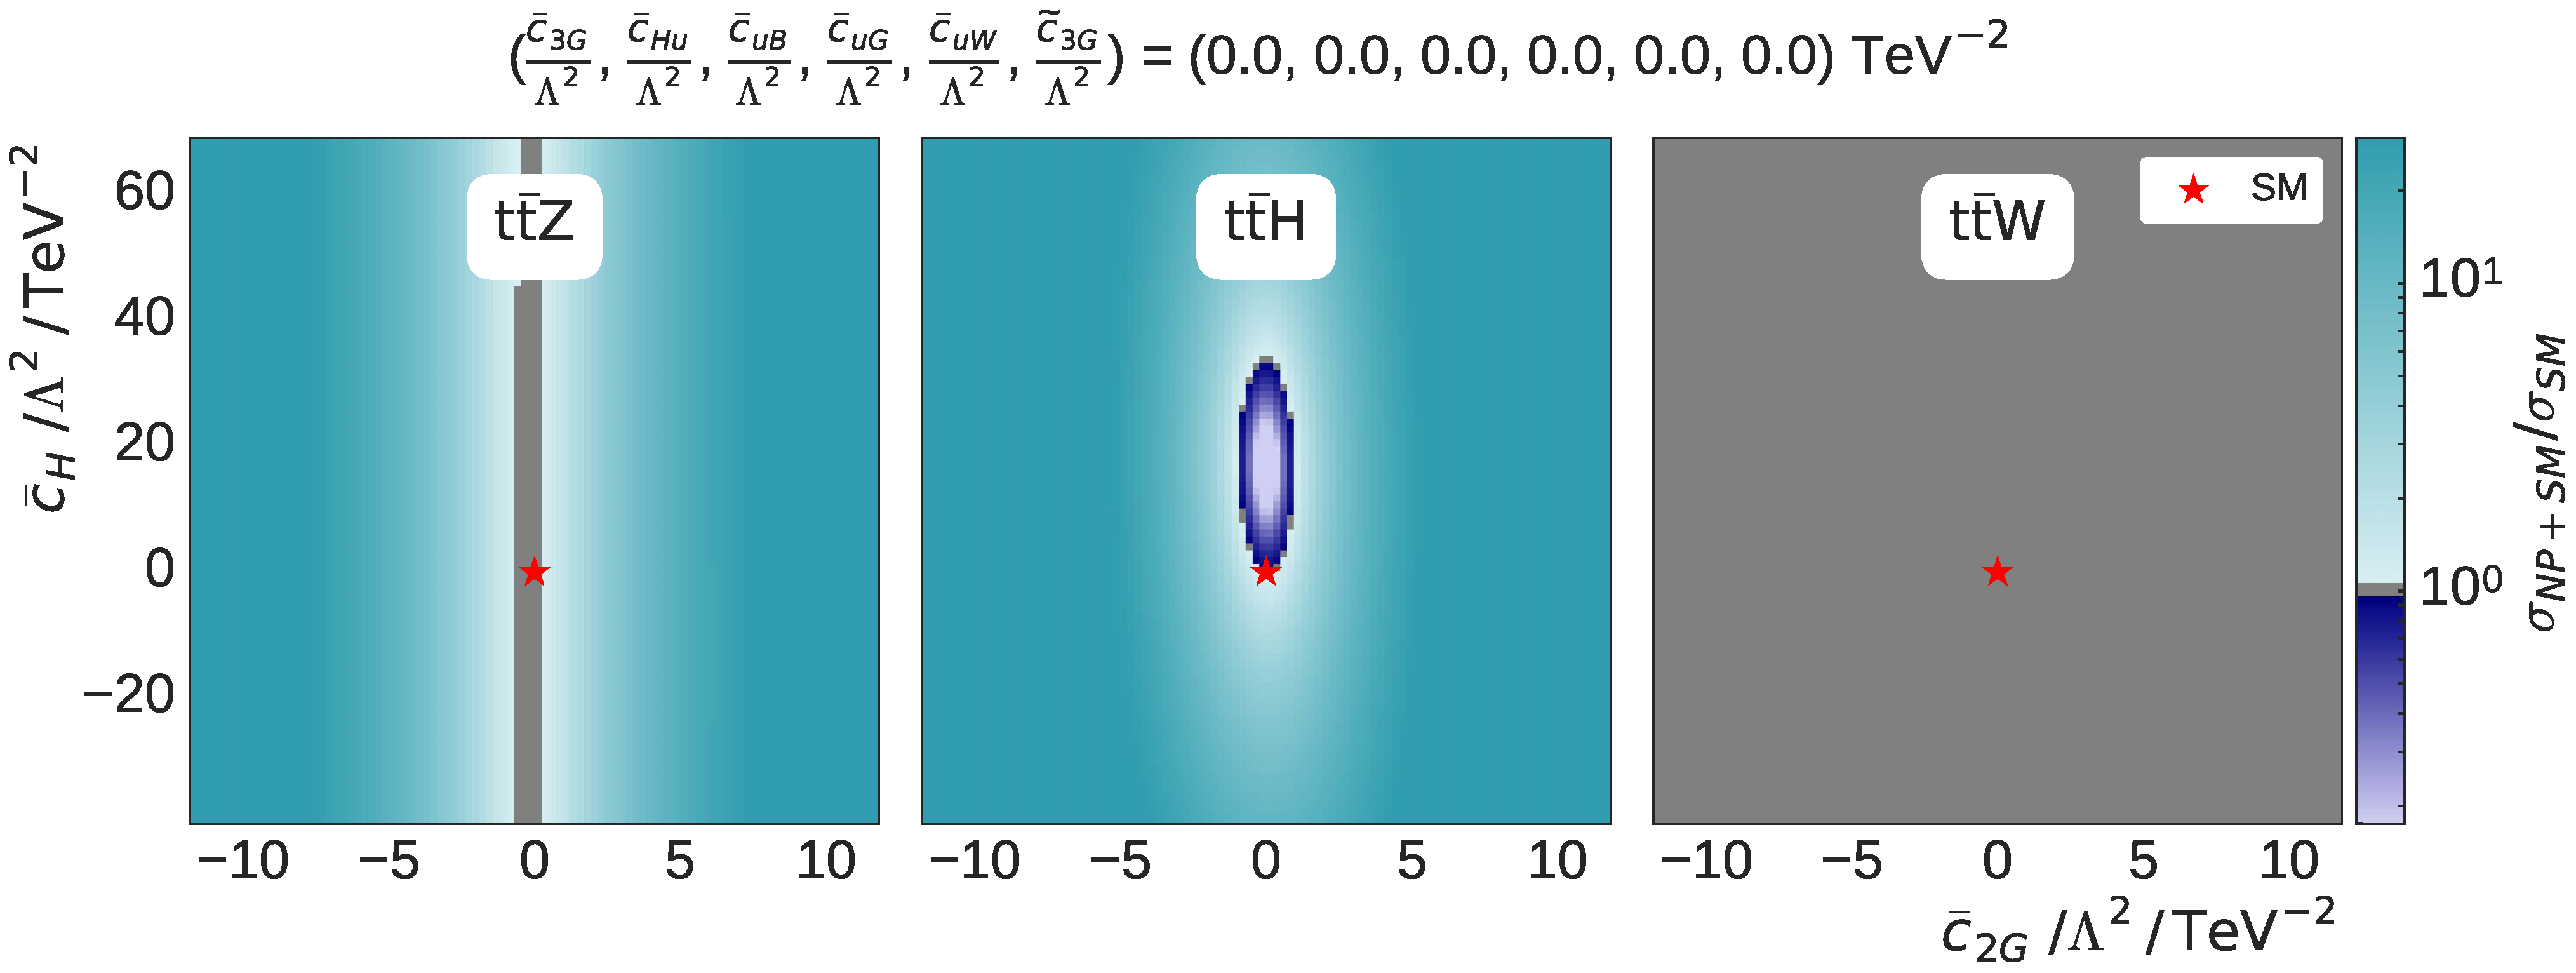
\includegraphics[width=\linewidth]{figures/thirteen-TeV/scaling-frozen/c2G_cH}
    \caption{}
  \end{subfigure}
  \begin{subfigure}{\linewidth}
    \centering
    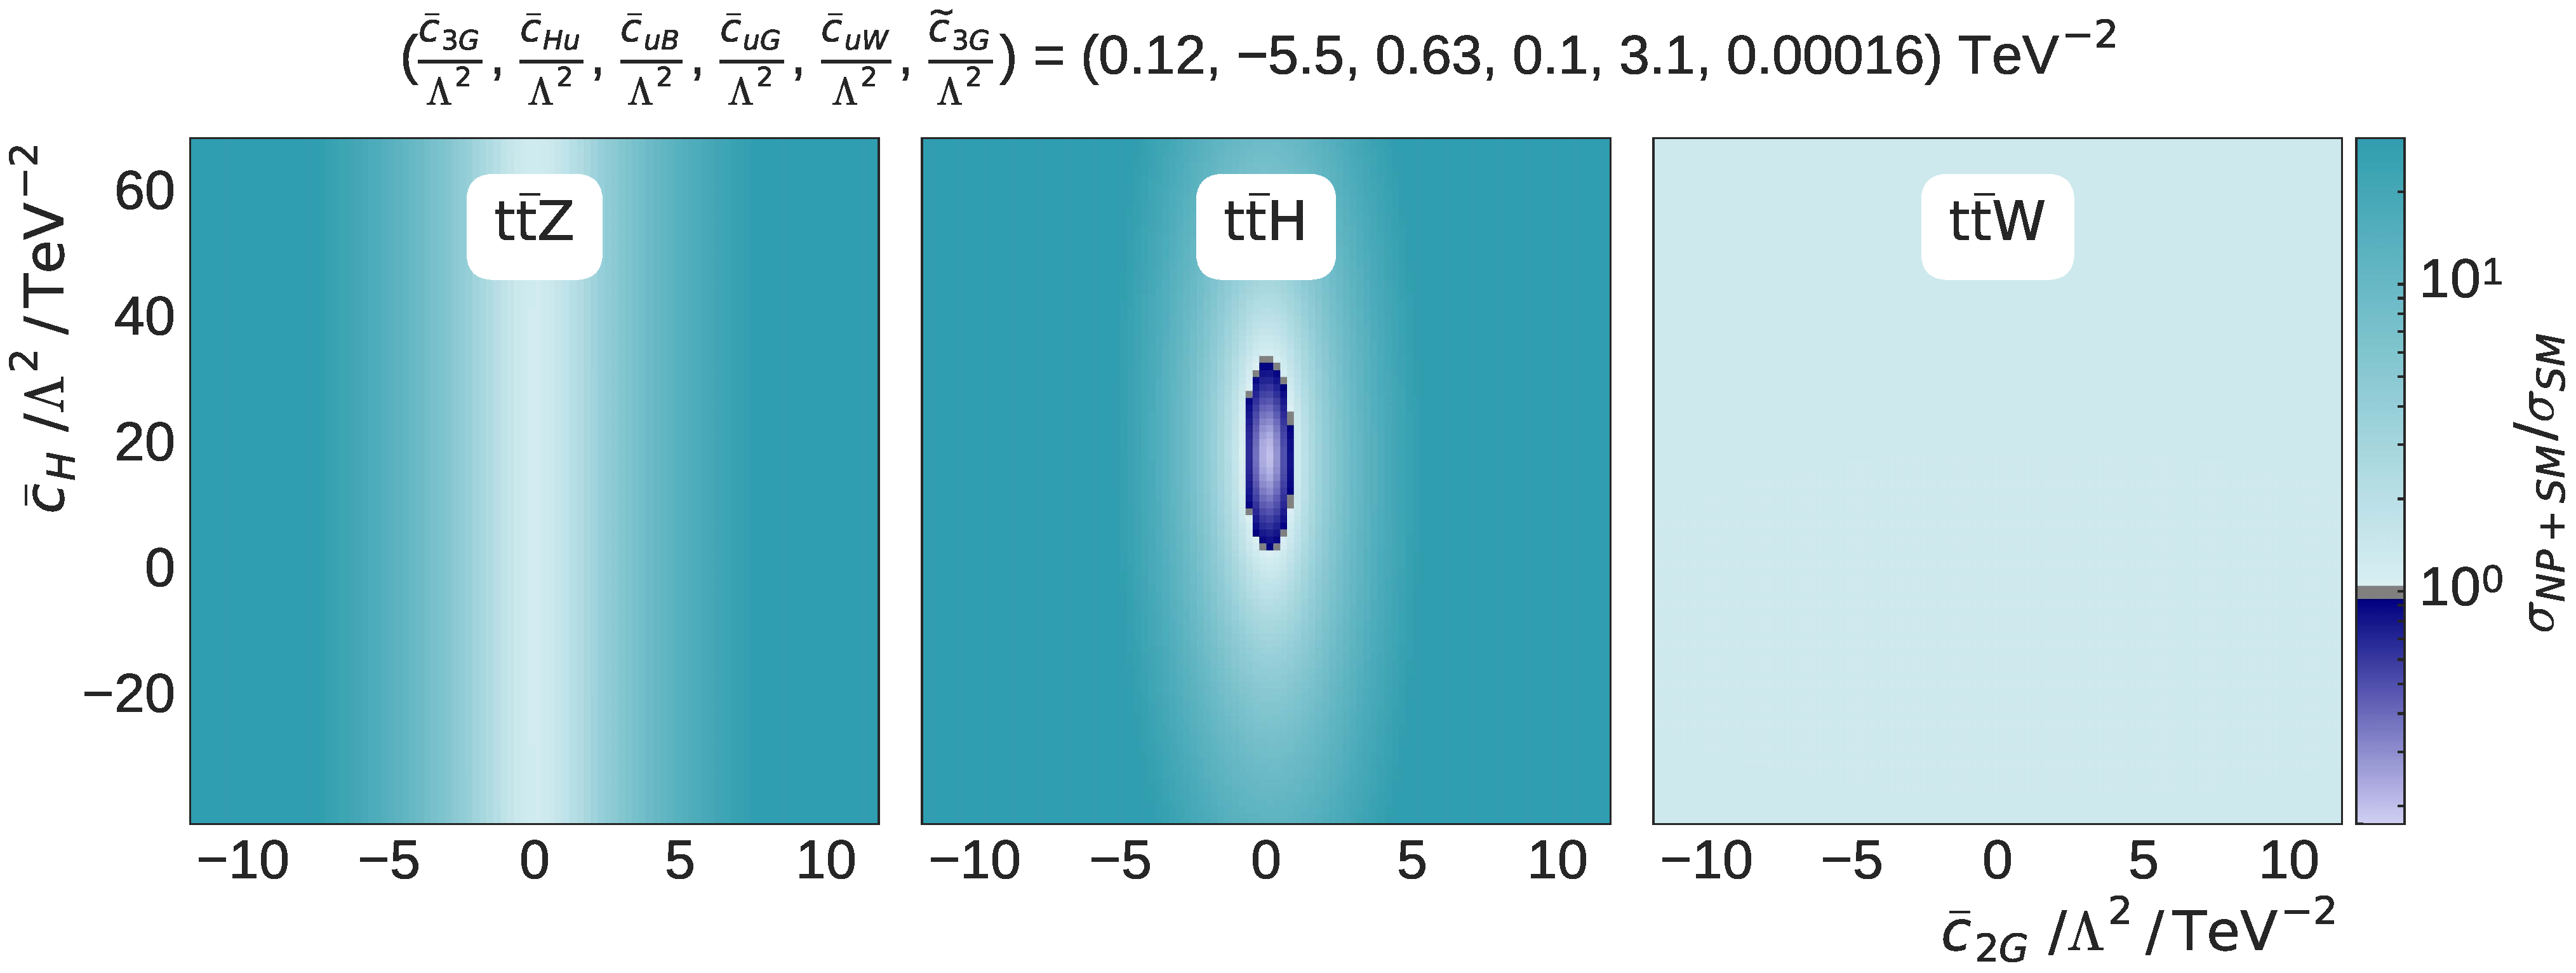
\includegraphics[width=\linewidth]{figures/thirteen-TeV/scaling/c2G_cH}
    \caption{}
  \end{subfigure}
  \begin{subfigure}{\linewidth}
    \centering
    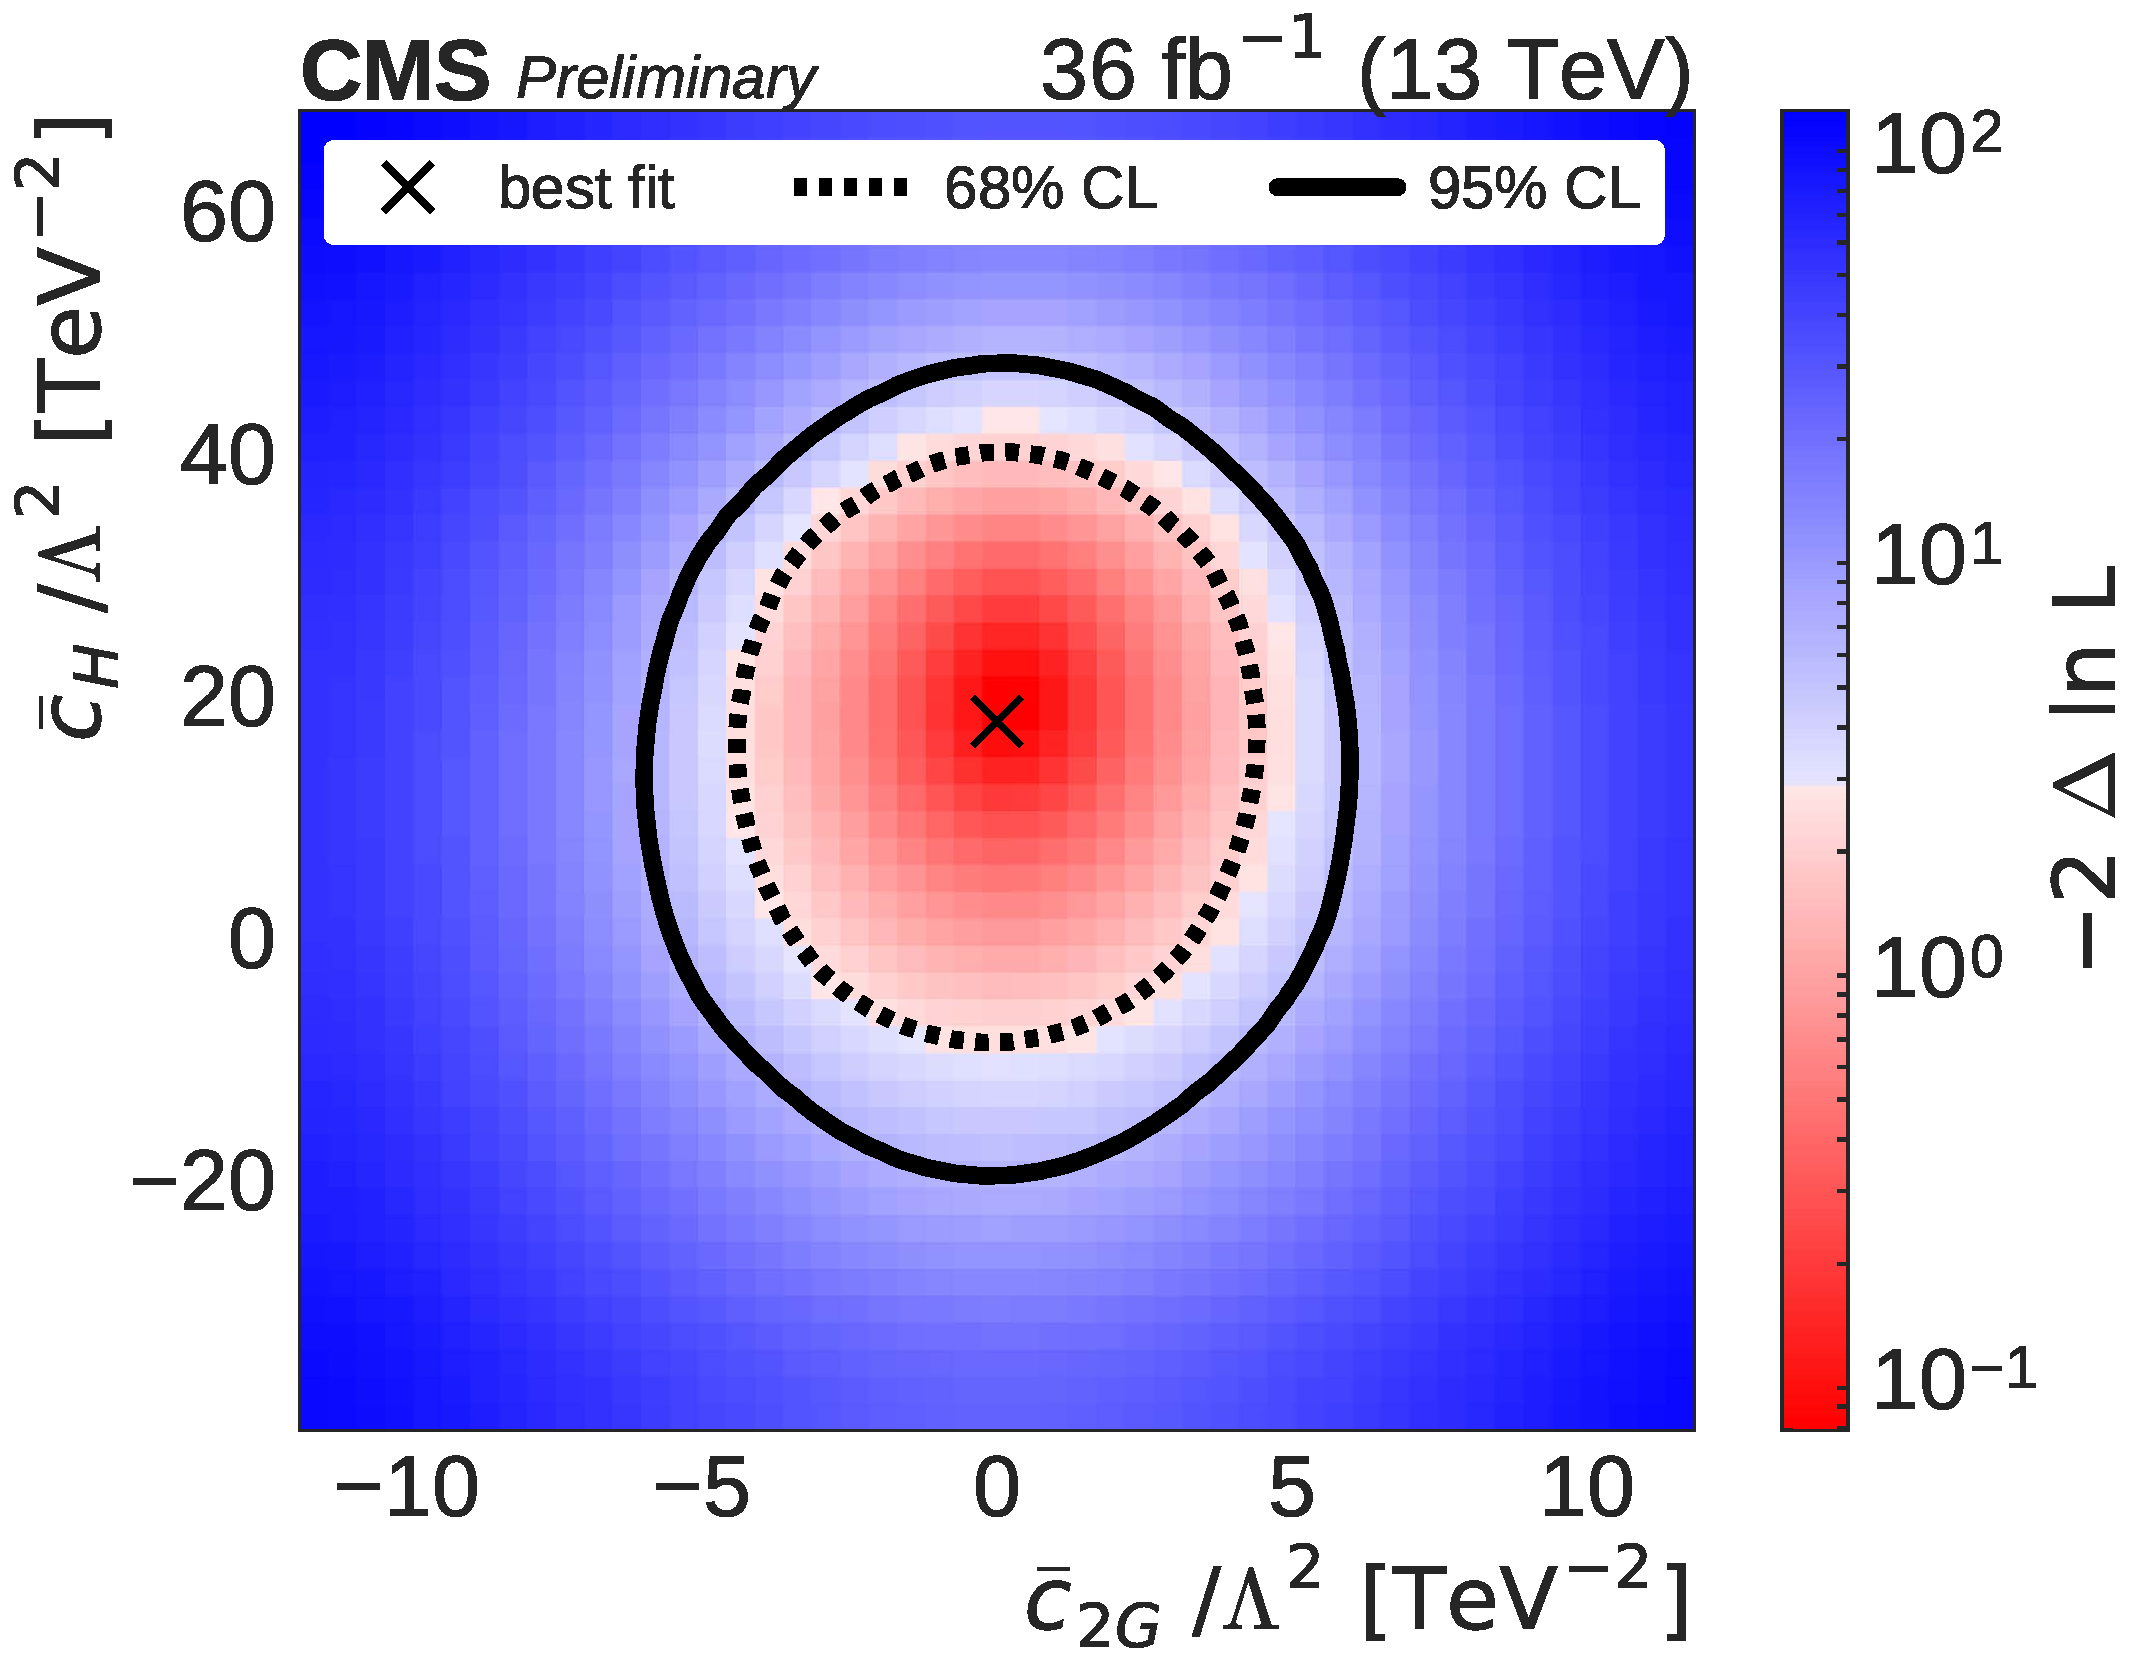
\includegraphics[width=0.6\linewidth]{figures/thirteen-TeV/nll/c2G_cH}
    \caption{}
  \end{subfigure}
  \vspace{-1cm}
  \setlength{\capwidth}{15cm}
  \caption[Signal scaling and profile likelihood scan in the \cH, \ctwoG plane]{Signal scaling shown
  in the \cH, \ctwoG plane with all other coefficients fixed to zero (a) to their best-fit values
  (b) for \ttZ (left), \ttH (center), and \ttW (right). The color represents the scaling

  ($\sigma_\text{NP + SM} / \sigma_\text{SM}$) due to NP effects. The star represents the SM point in
  which all $c_i=0$. The negative log likelihood is shown in (c). The best fit is represented by a
  cross. The \SI{68}{\percent} and \SI{95}{\percent} CL contours are shown with dashed and solid
  lines, respectively.}
\end{figure}

\begin{figure}
  \vspace{-1cm}
  \begin{subfigure}{\linewidth}
    \centering
    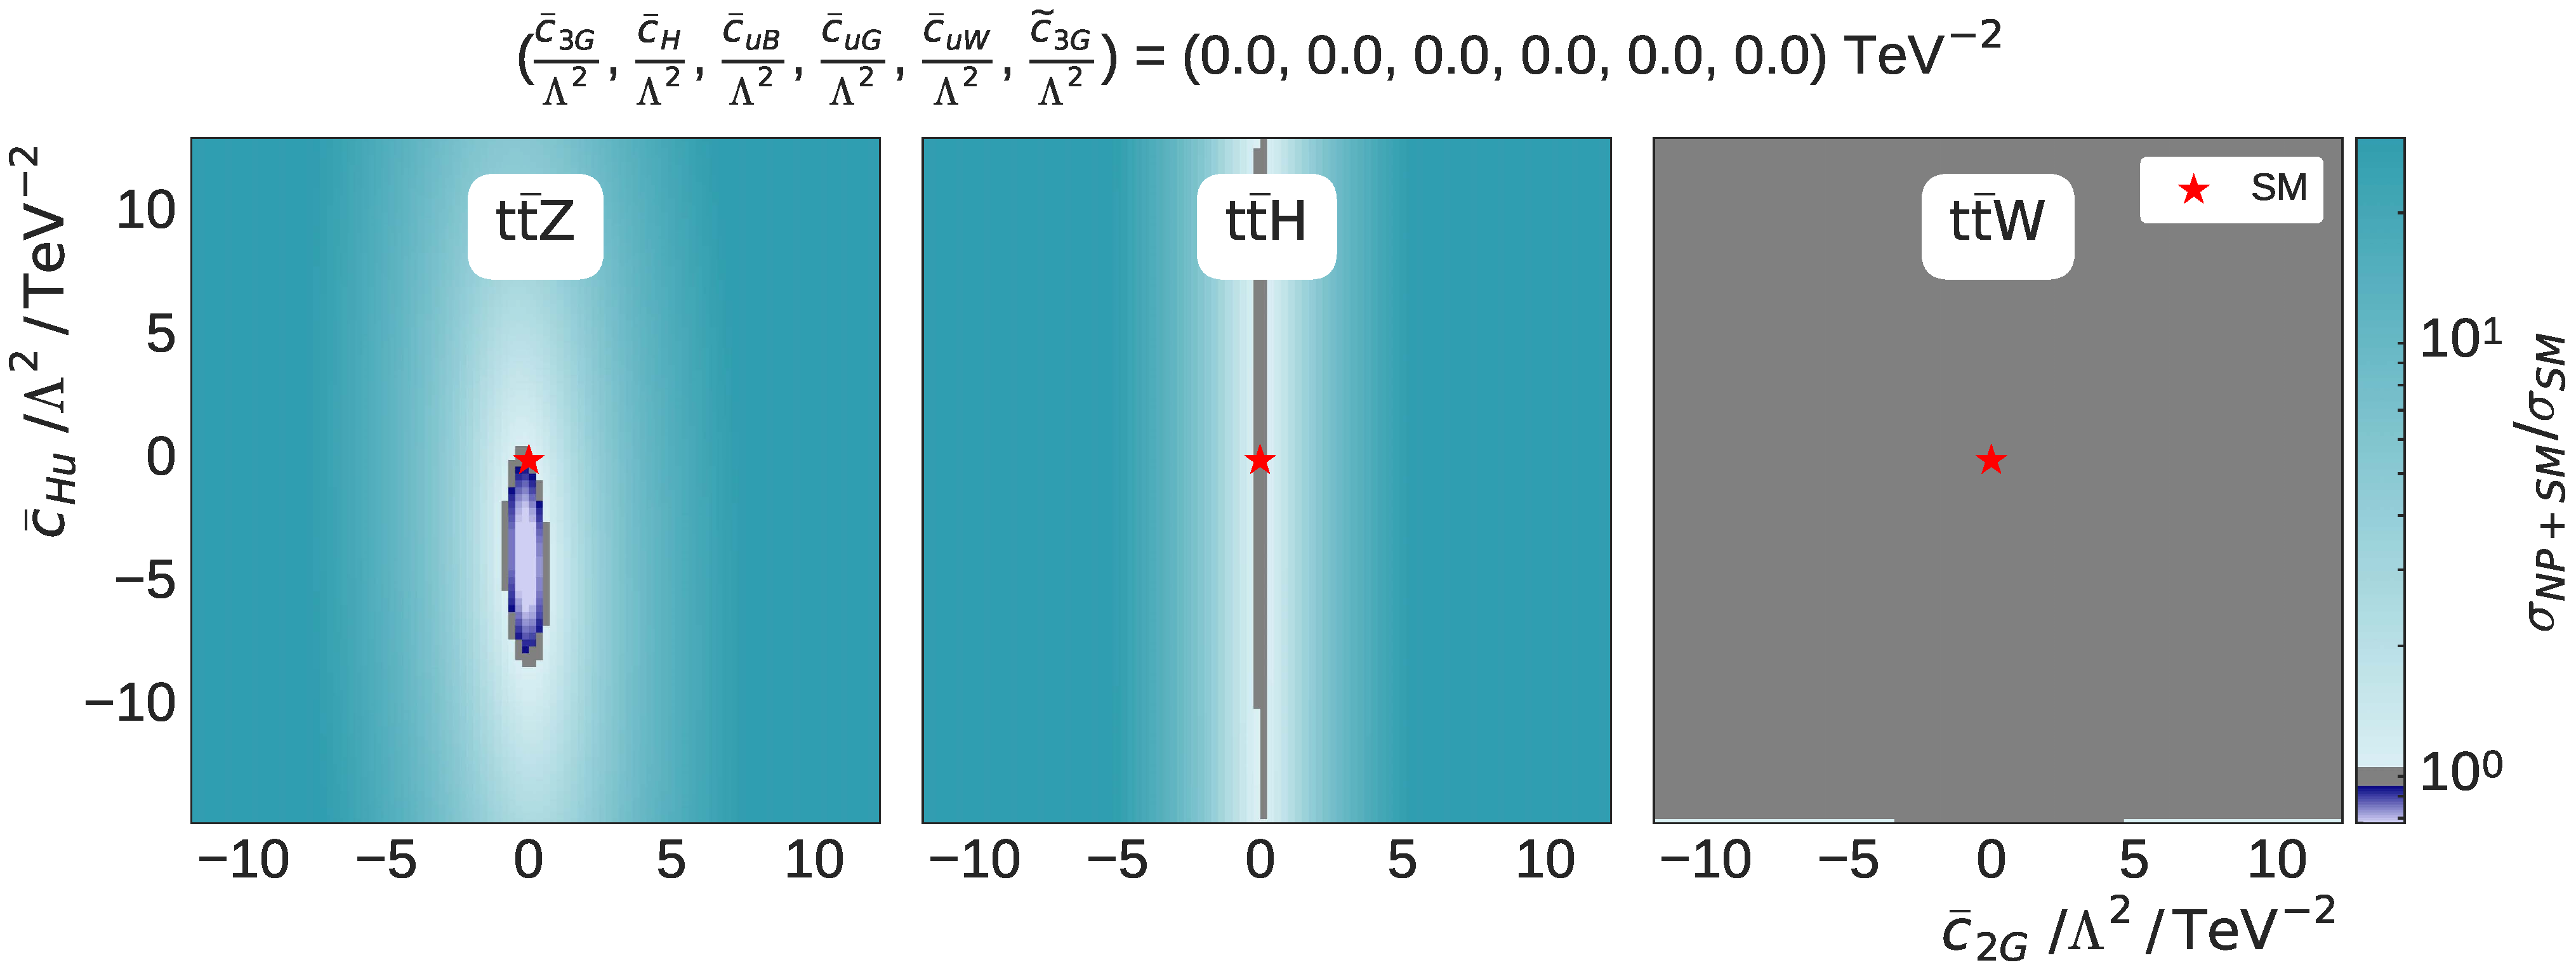
\includegraphics[width=\linewidth]{figures/thirteen-TeV/scaling-frozen/c2G_cHu}
    \caption{}
  \end{subfigure}
  \begin{subfigure}{\linewidth}
    \centering
    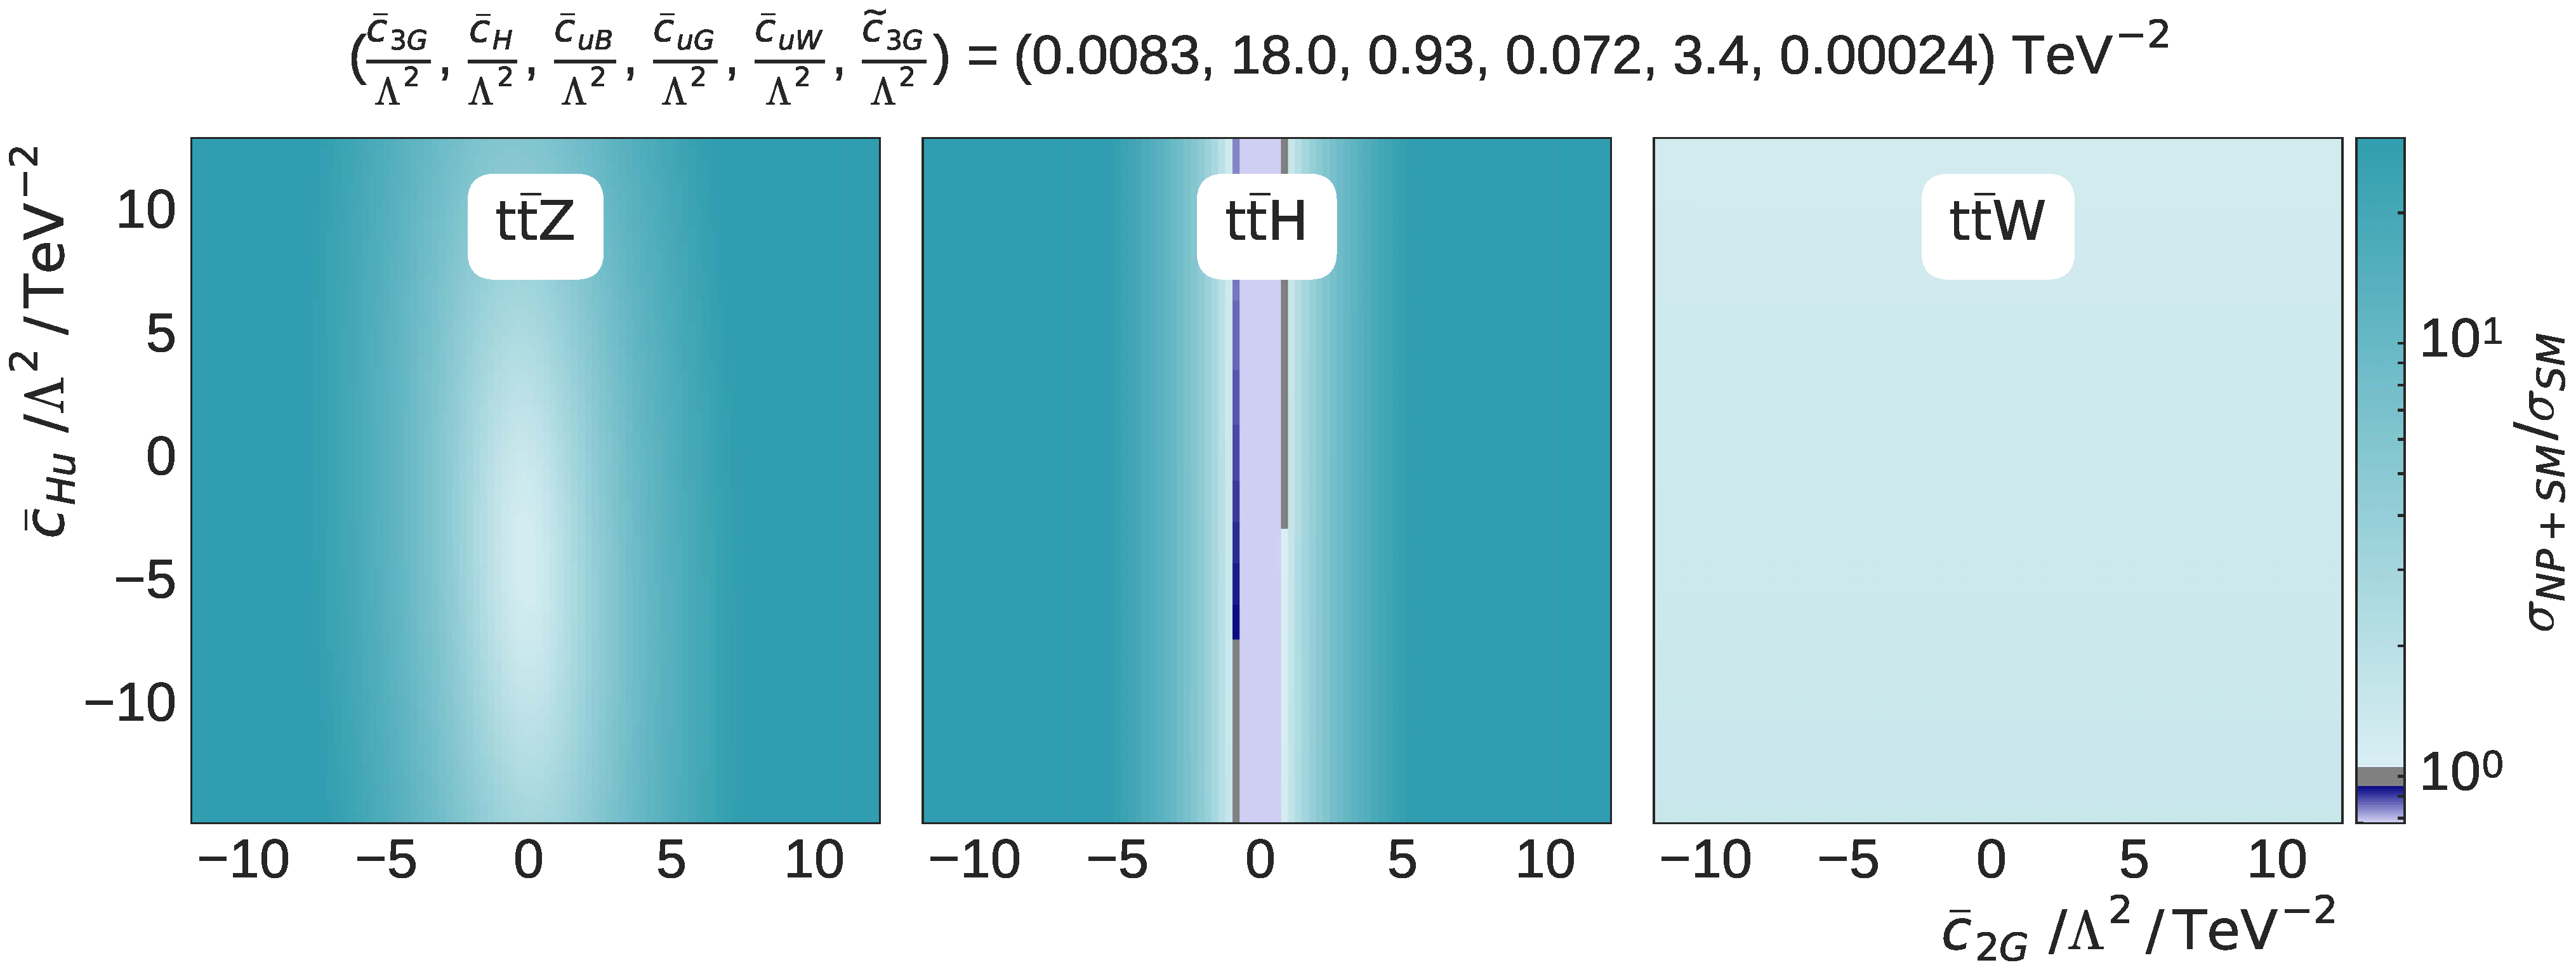
\includegraphics[width=\linewidth]{figures/thirteen-TeV/scaling/c2G_cHu}
    \caption{}
  \end{subfigure}
  \begin{subfigure}{\linewidth}
    \centering
    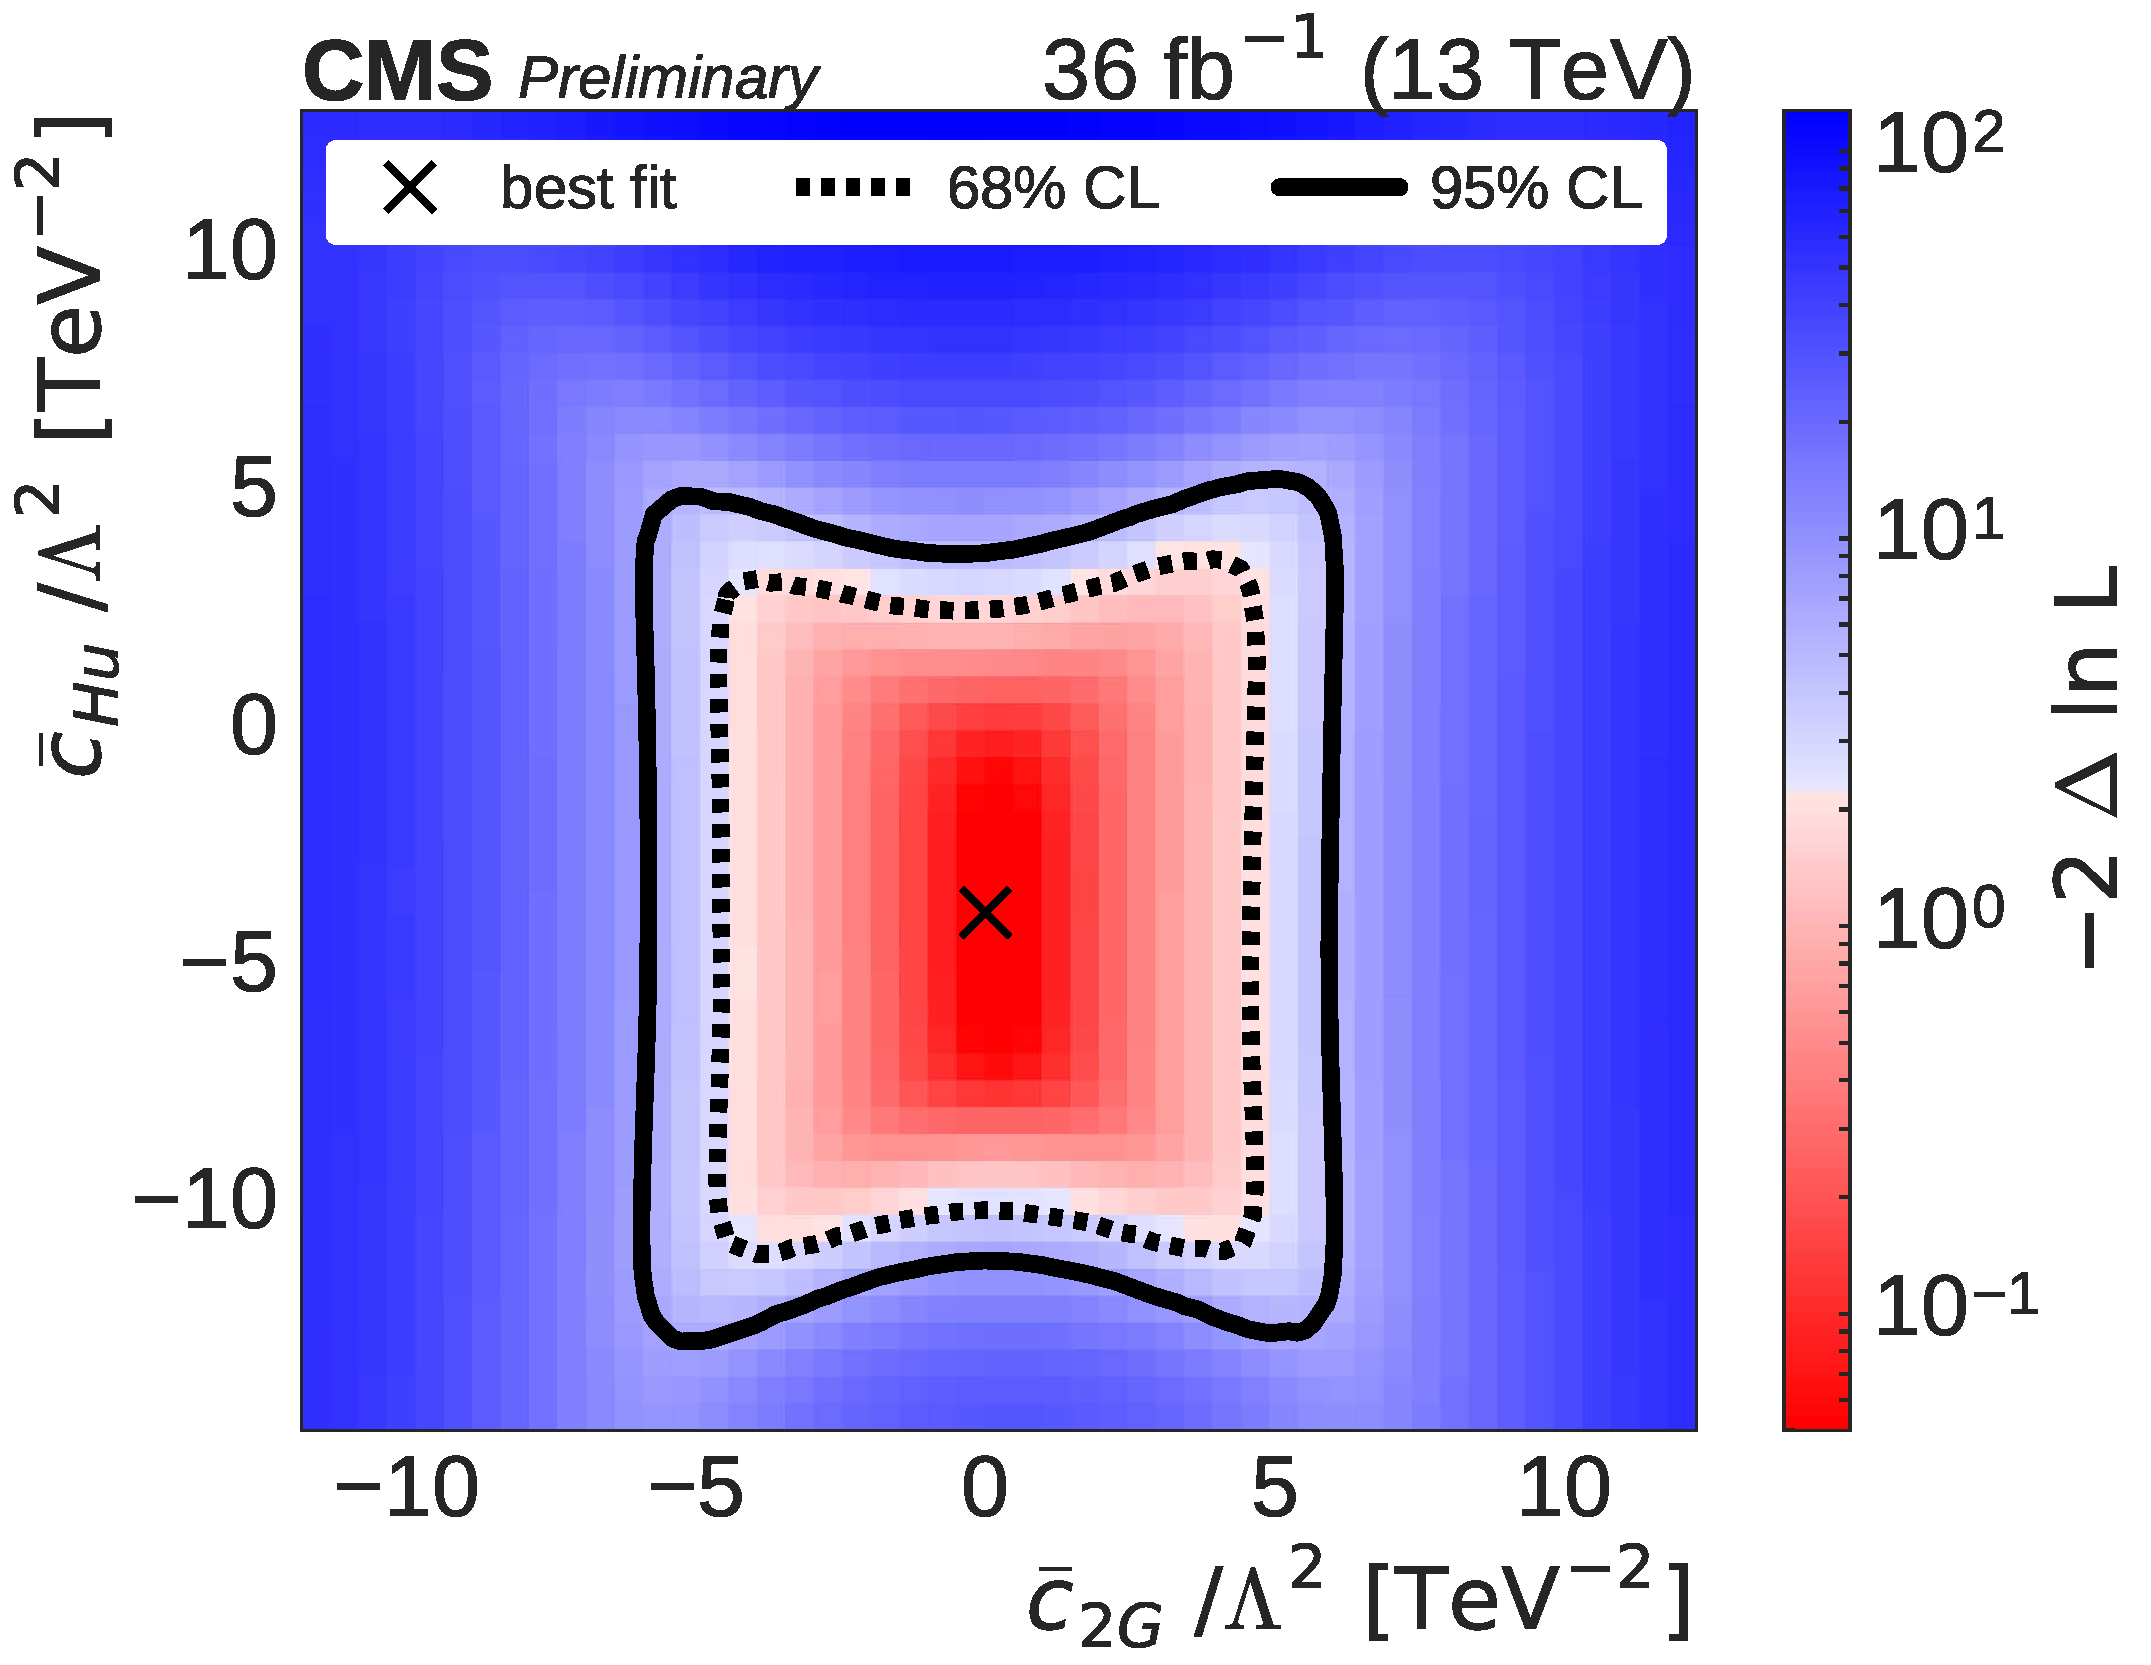
\includegraphics[width=0.6\linewidth]{figures/thirteen-TeV/nll/c2G_cHu}
    \caption{}
  \end{subfigure}
  \vspace{-1cm}
  \setlength{\capwidth}{15cm}
  \setlength{\capwidth}{15cm}
  \caption[Signal scaling and profile likelihood scan in the \cHu, \ctwoG plane]{Signal scaling
    shown in the \cHu, \ctwoG plane with all other coefficients fixed to zero (a) to their best-fit
    values (b) for \ttZ (left), \ttH (center), and \ttW (right). The color represents the scaling
    ($\sigma_\text{NP + SM} / \sigma_\text{SM}$) due to NP effects. The star represents the SM point
    in which all $c_i=0$. The negative log likelihood is shown in (c). The best fit is represented
    by a cross. The \SI{68}{\percent} and \SI{95}{\percent} CL contours are shown with dashed and
    solid lines, respectively.}
\end{figure}

\begin{figure}
  \vspace{-1cm}
  \begin{subfigure}{\linewidth}
    \centering
    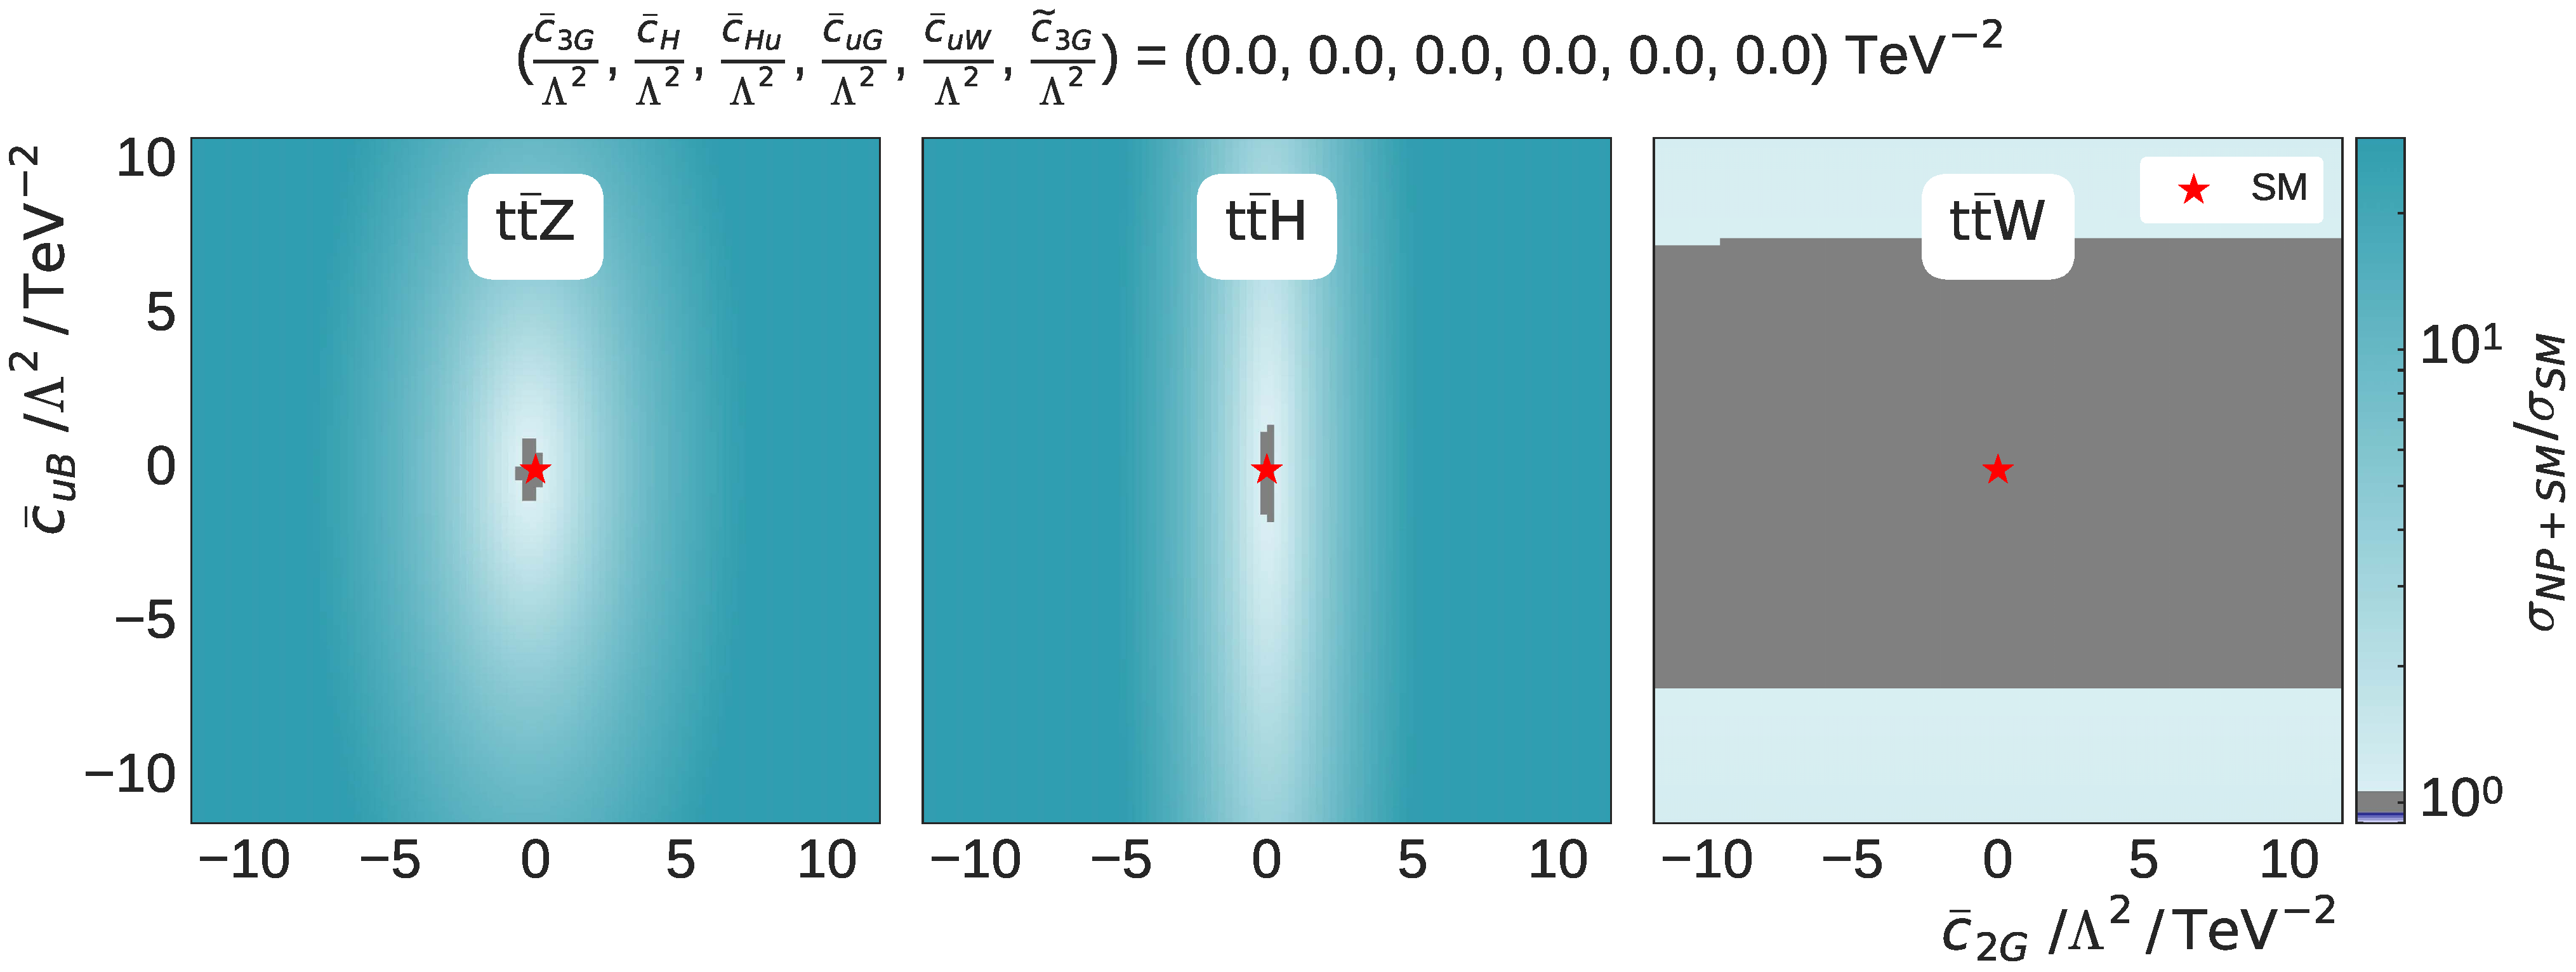
\includegraphics[width=\linewidth]{figures/thirteen-TeV/scaling-frozen/c2G_cuB}
    \caption{}
  \end{subfigure}
  \begin{subfigure}{\linewidth}
    \centering
    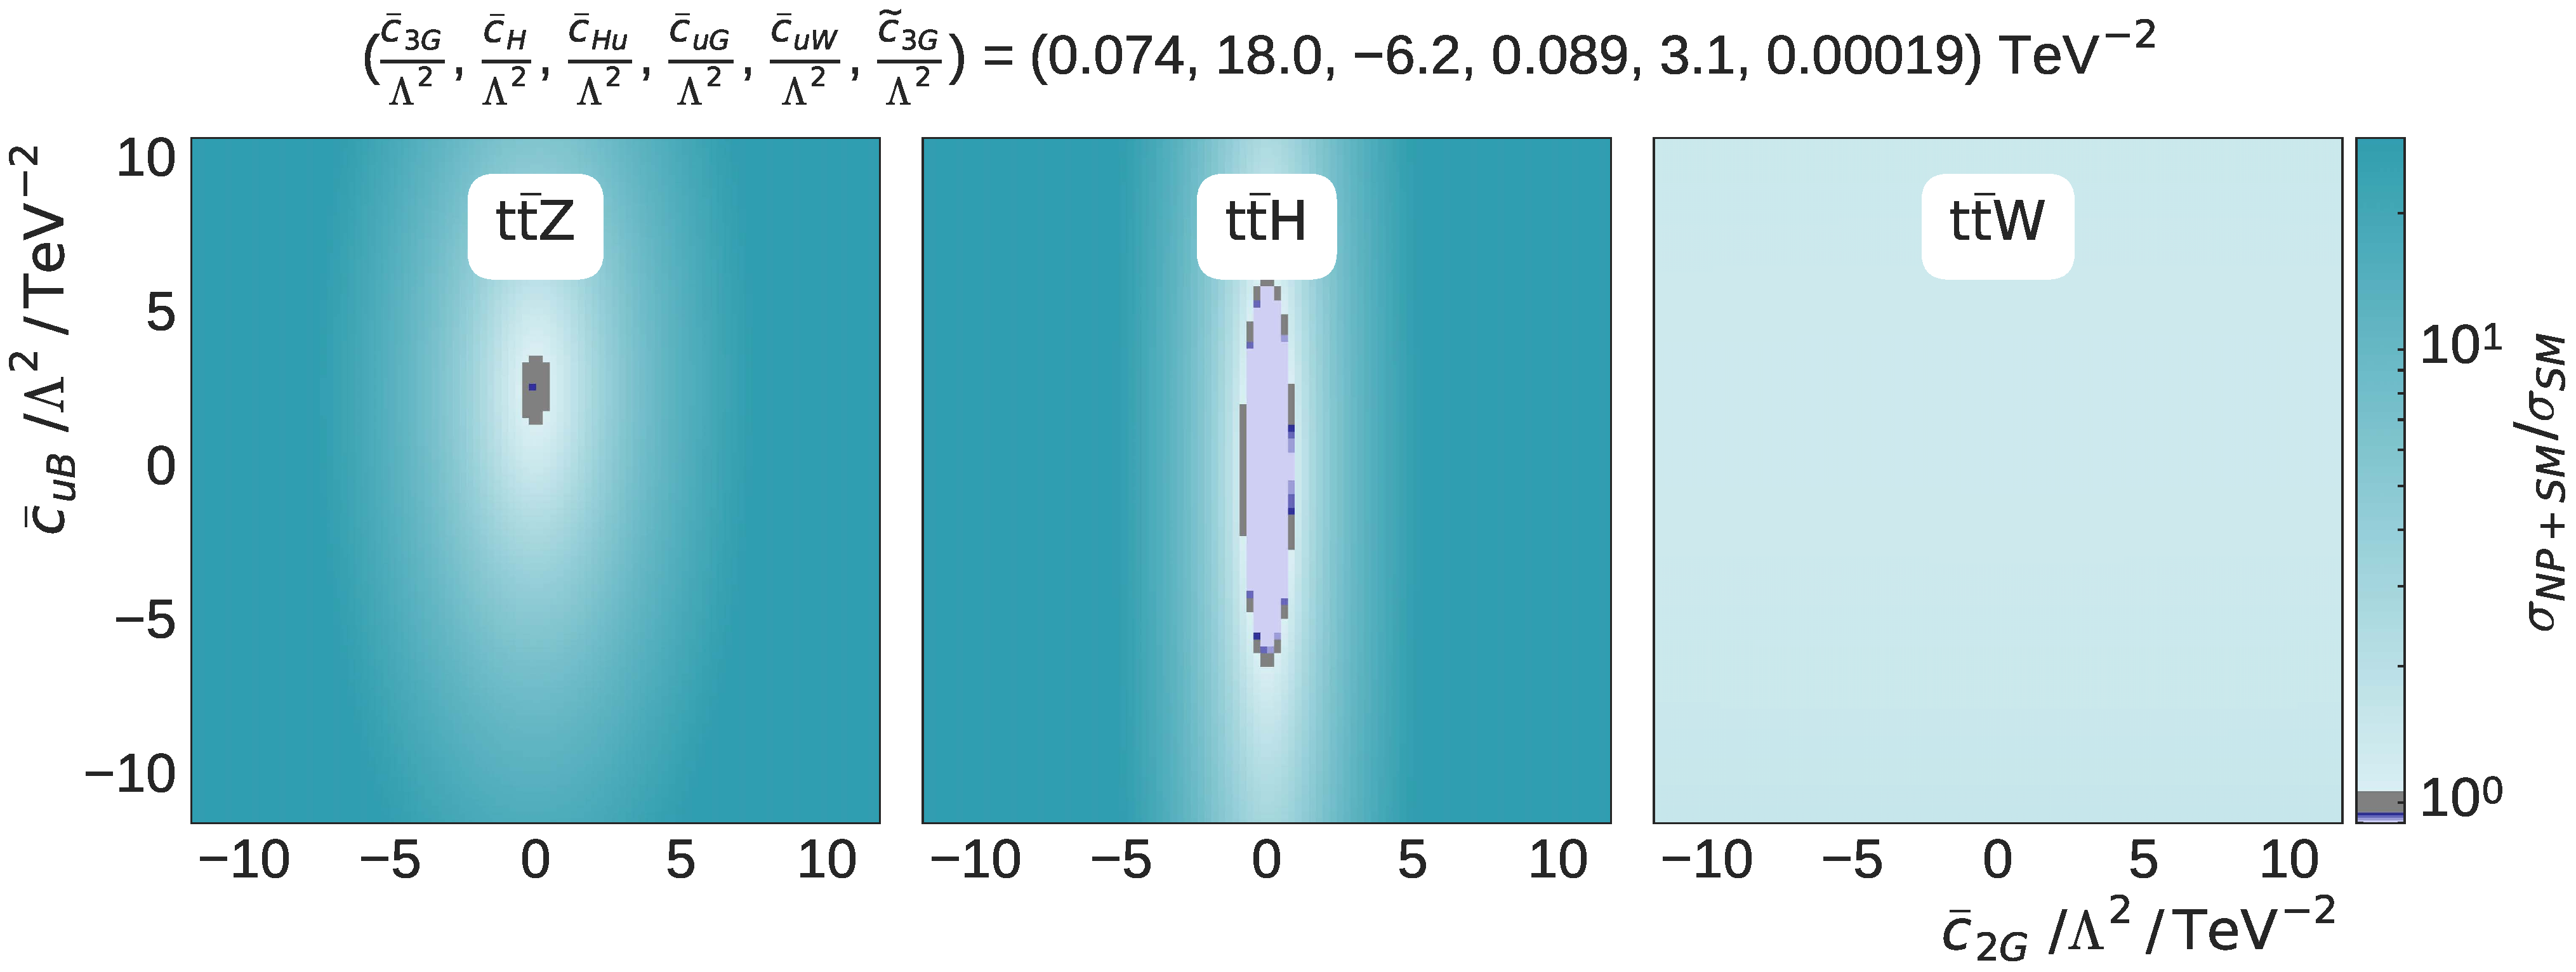
\includegraphics[width=\linewidth]{figures/thirteen-TeV/scaling/c2G_cuB}
    \caption{}
  \end{subfigure}
  \begin{subfigure}{\linewidth}
    \centering
    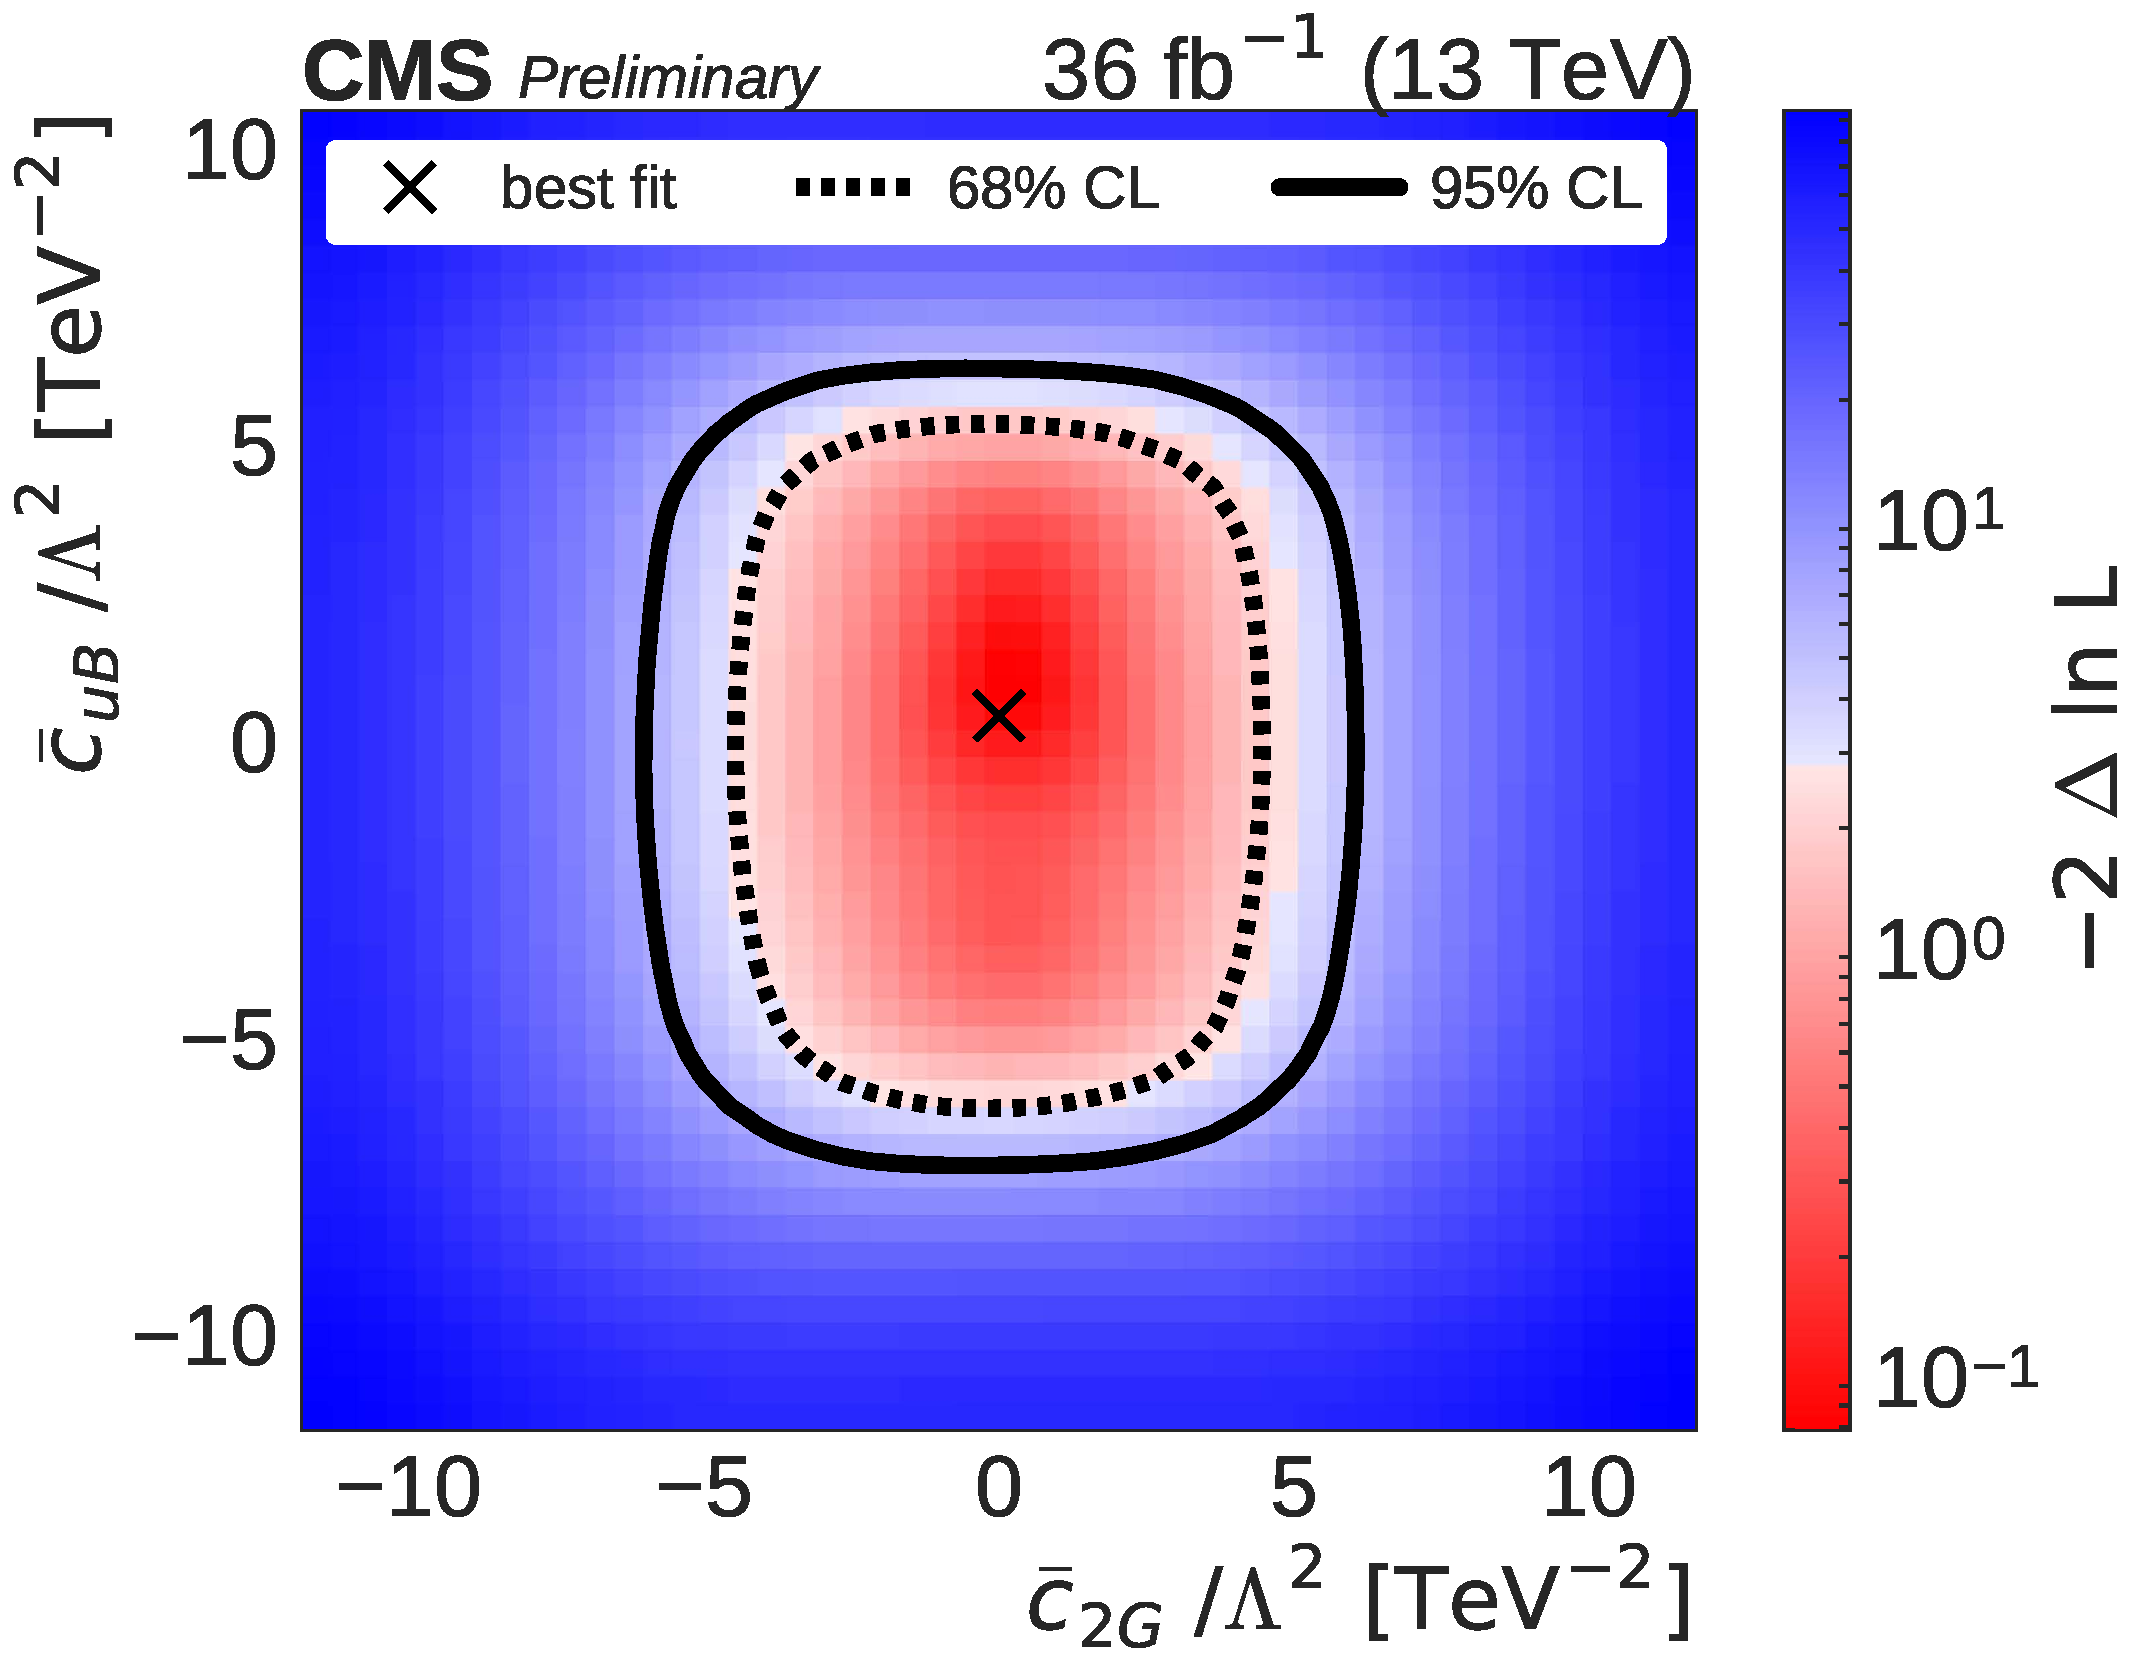
\includegraphics[width=0.6\linewidth]{figures/thirteen-TeV/nll/c2G_cuB}
    \caption{}
  \end{subfigure}
  \vspace{-1cm}
  \setlength{\capwidth}{15cm}
  \caption[Signal scaling and profile likelihood scan in the \ctwoG, \cuB plane]{Signal scaling
    shown in the \ctwoG, \cuB plane with all other coefficients fixed to zero (a) or their best-fit
    values (b) for \ttZ (left), \ttH (center), and \ttW (right). The color represents the scaling
    ($\sigma_\text{NP + SM} / \sigma_\text{SM}$) due to NP effects. The star represents the SM point in
    which all $c_i=0$. The negative log likelihood is shown in (c). The best fit is represented by a
    cross. The \SI{68}{\percent} and \SI{95}{\percent} CL contours are shown with dashed and solid
  lines, respectively.}
\end{figure}

\begin{figure}
  \vspace{-1cm}
  \begin{subfigure}{\linewidth}
    \centering
    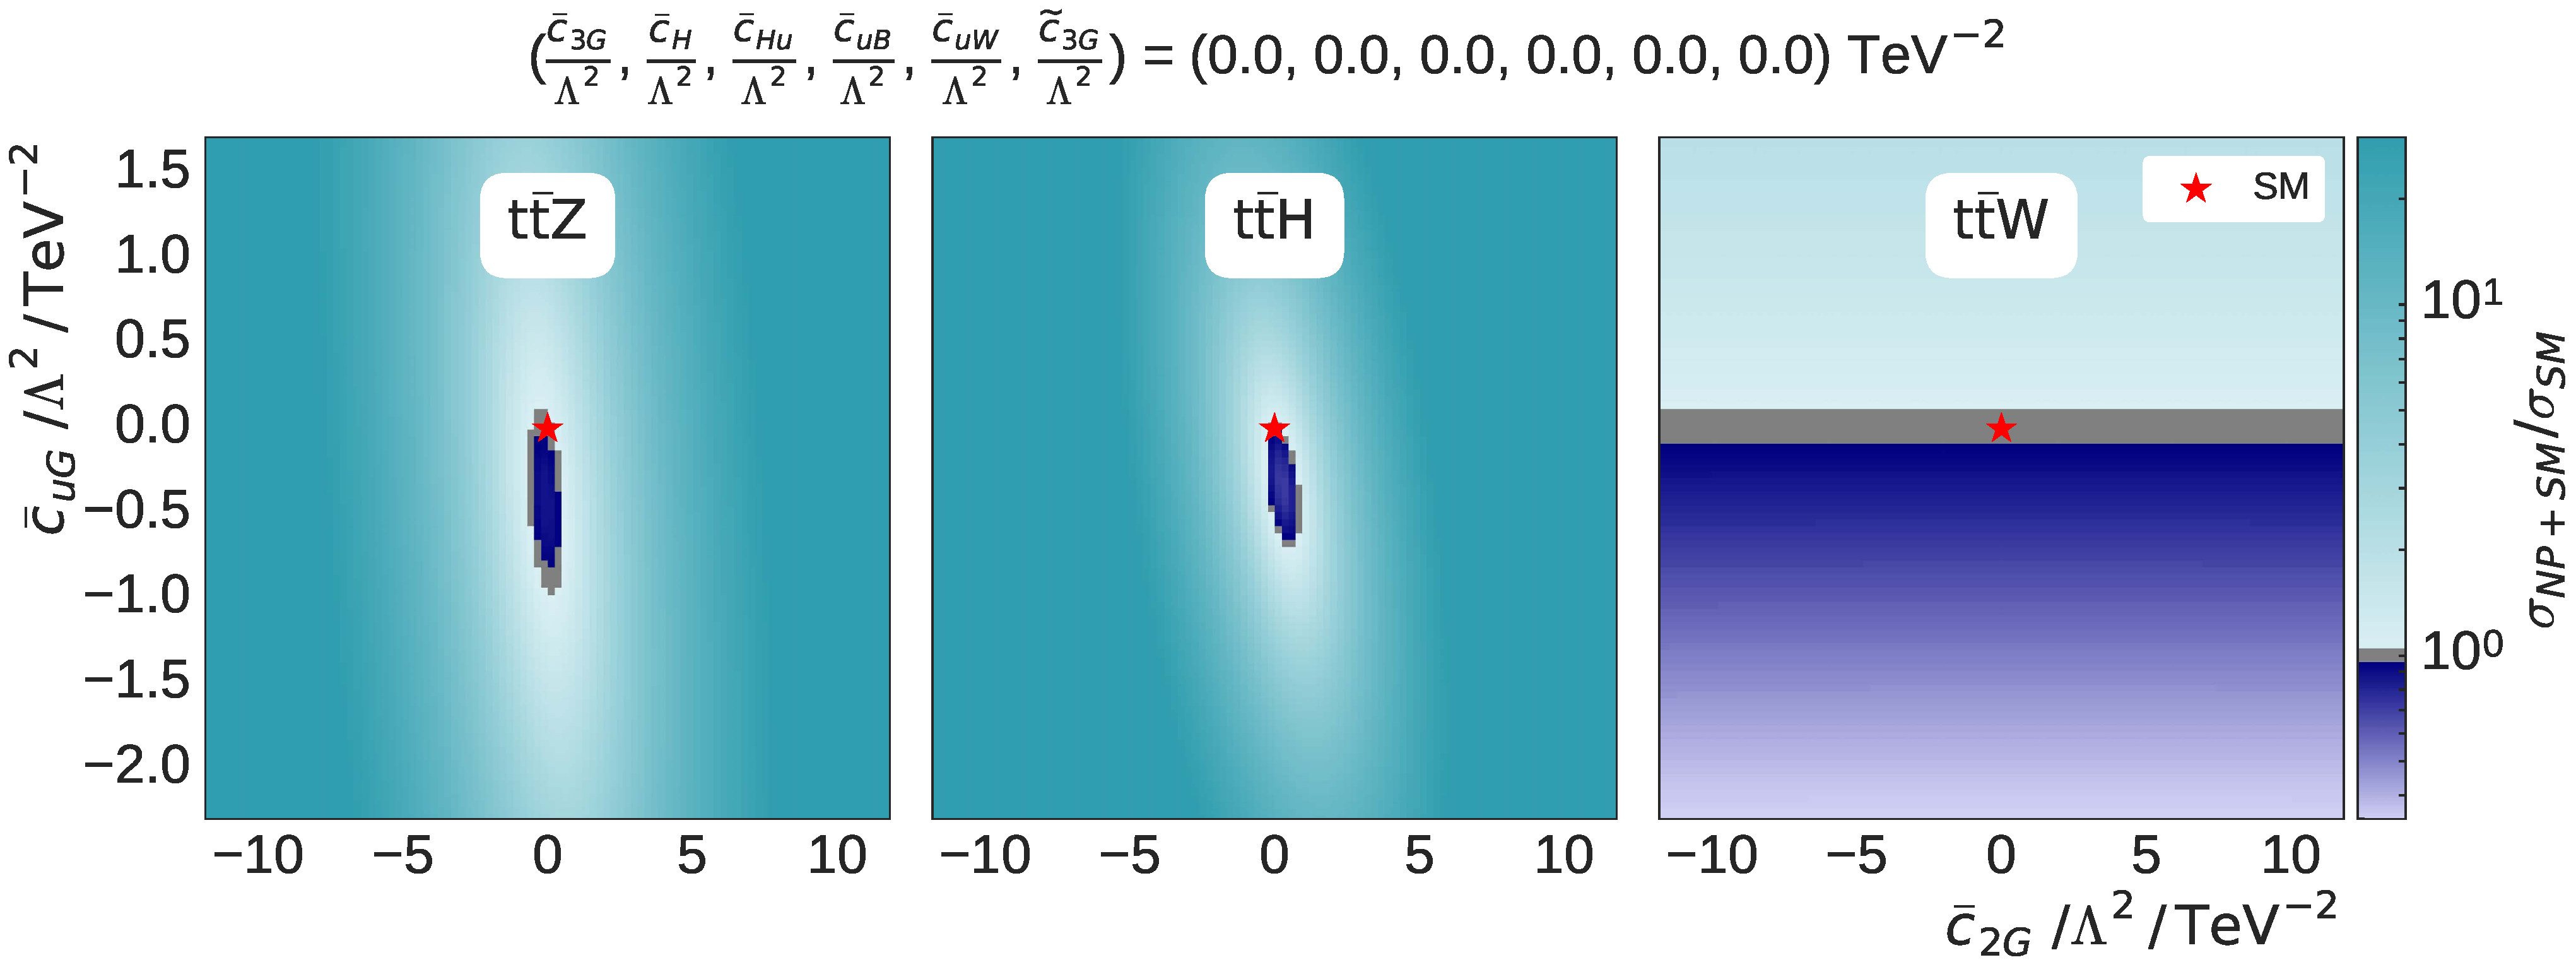
\includegraphics[width=\linewidth]{figures/thirteen-TeV/scaling-frozen/c2G_cuG}
    \caption{}
  \end{subfigure}
  \begin{subfigure}{\linewidth}
    \centering
    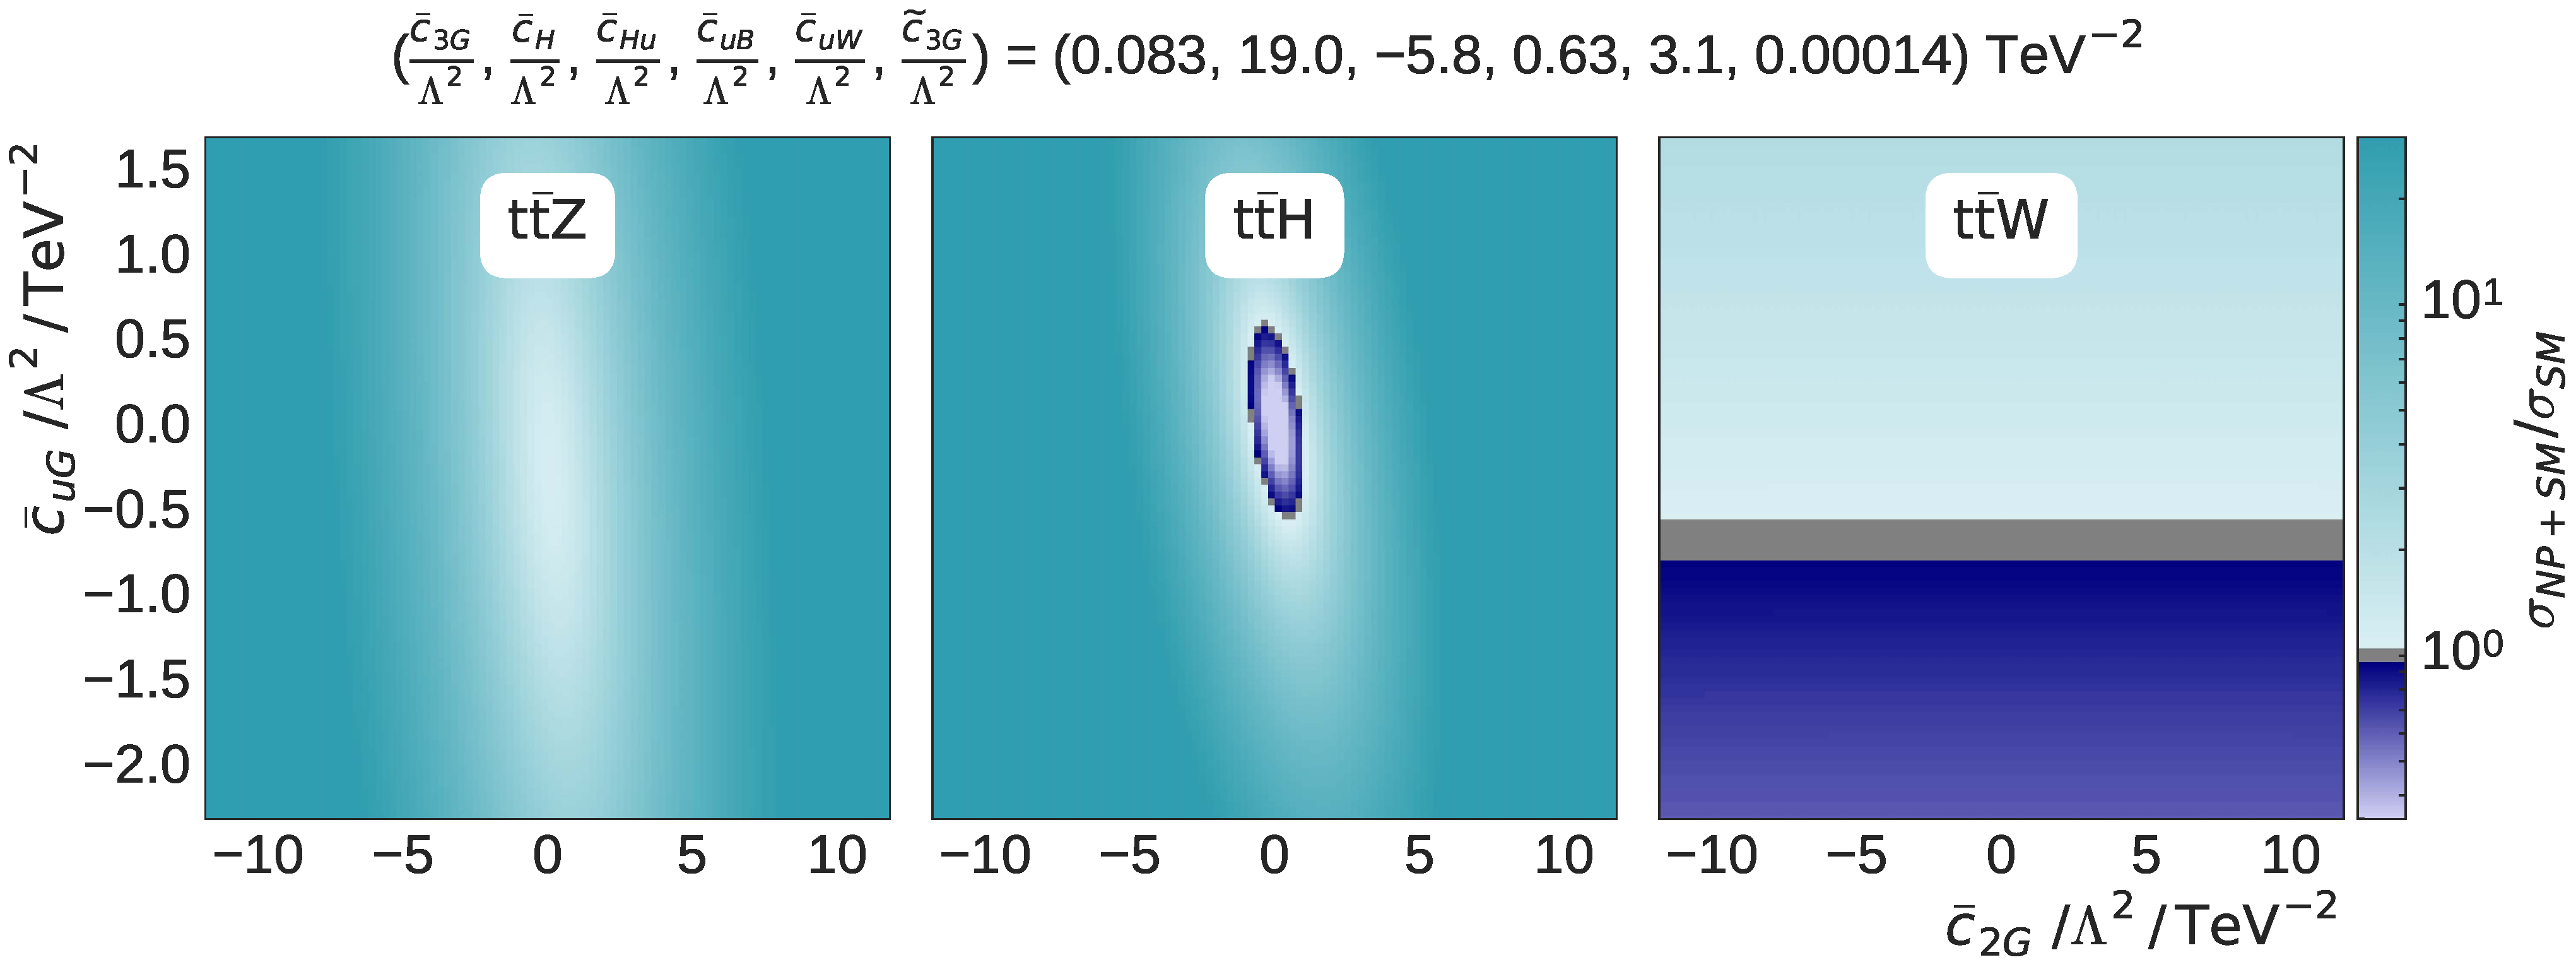
\includegraphics[width=\linewidth]{figures/thirteen-TeV/scaling/c2G_cuG}
    \caption{}
  \end{subfigure}
  \begin{subfigure}{\linewidth}
    \centering
    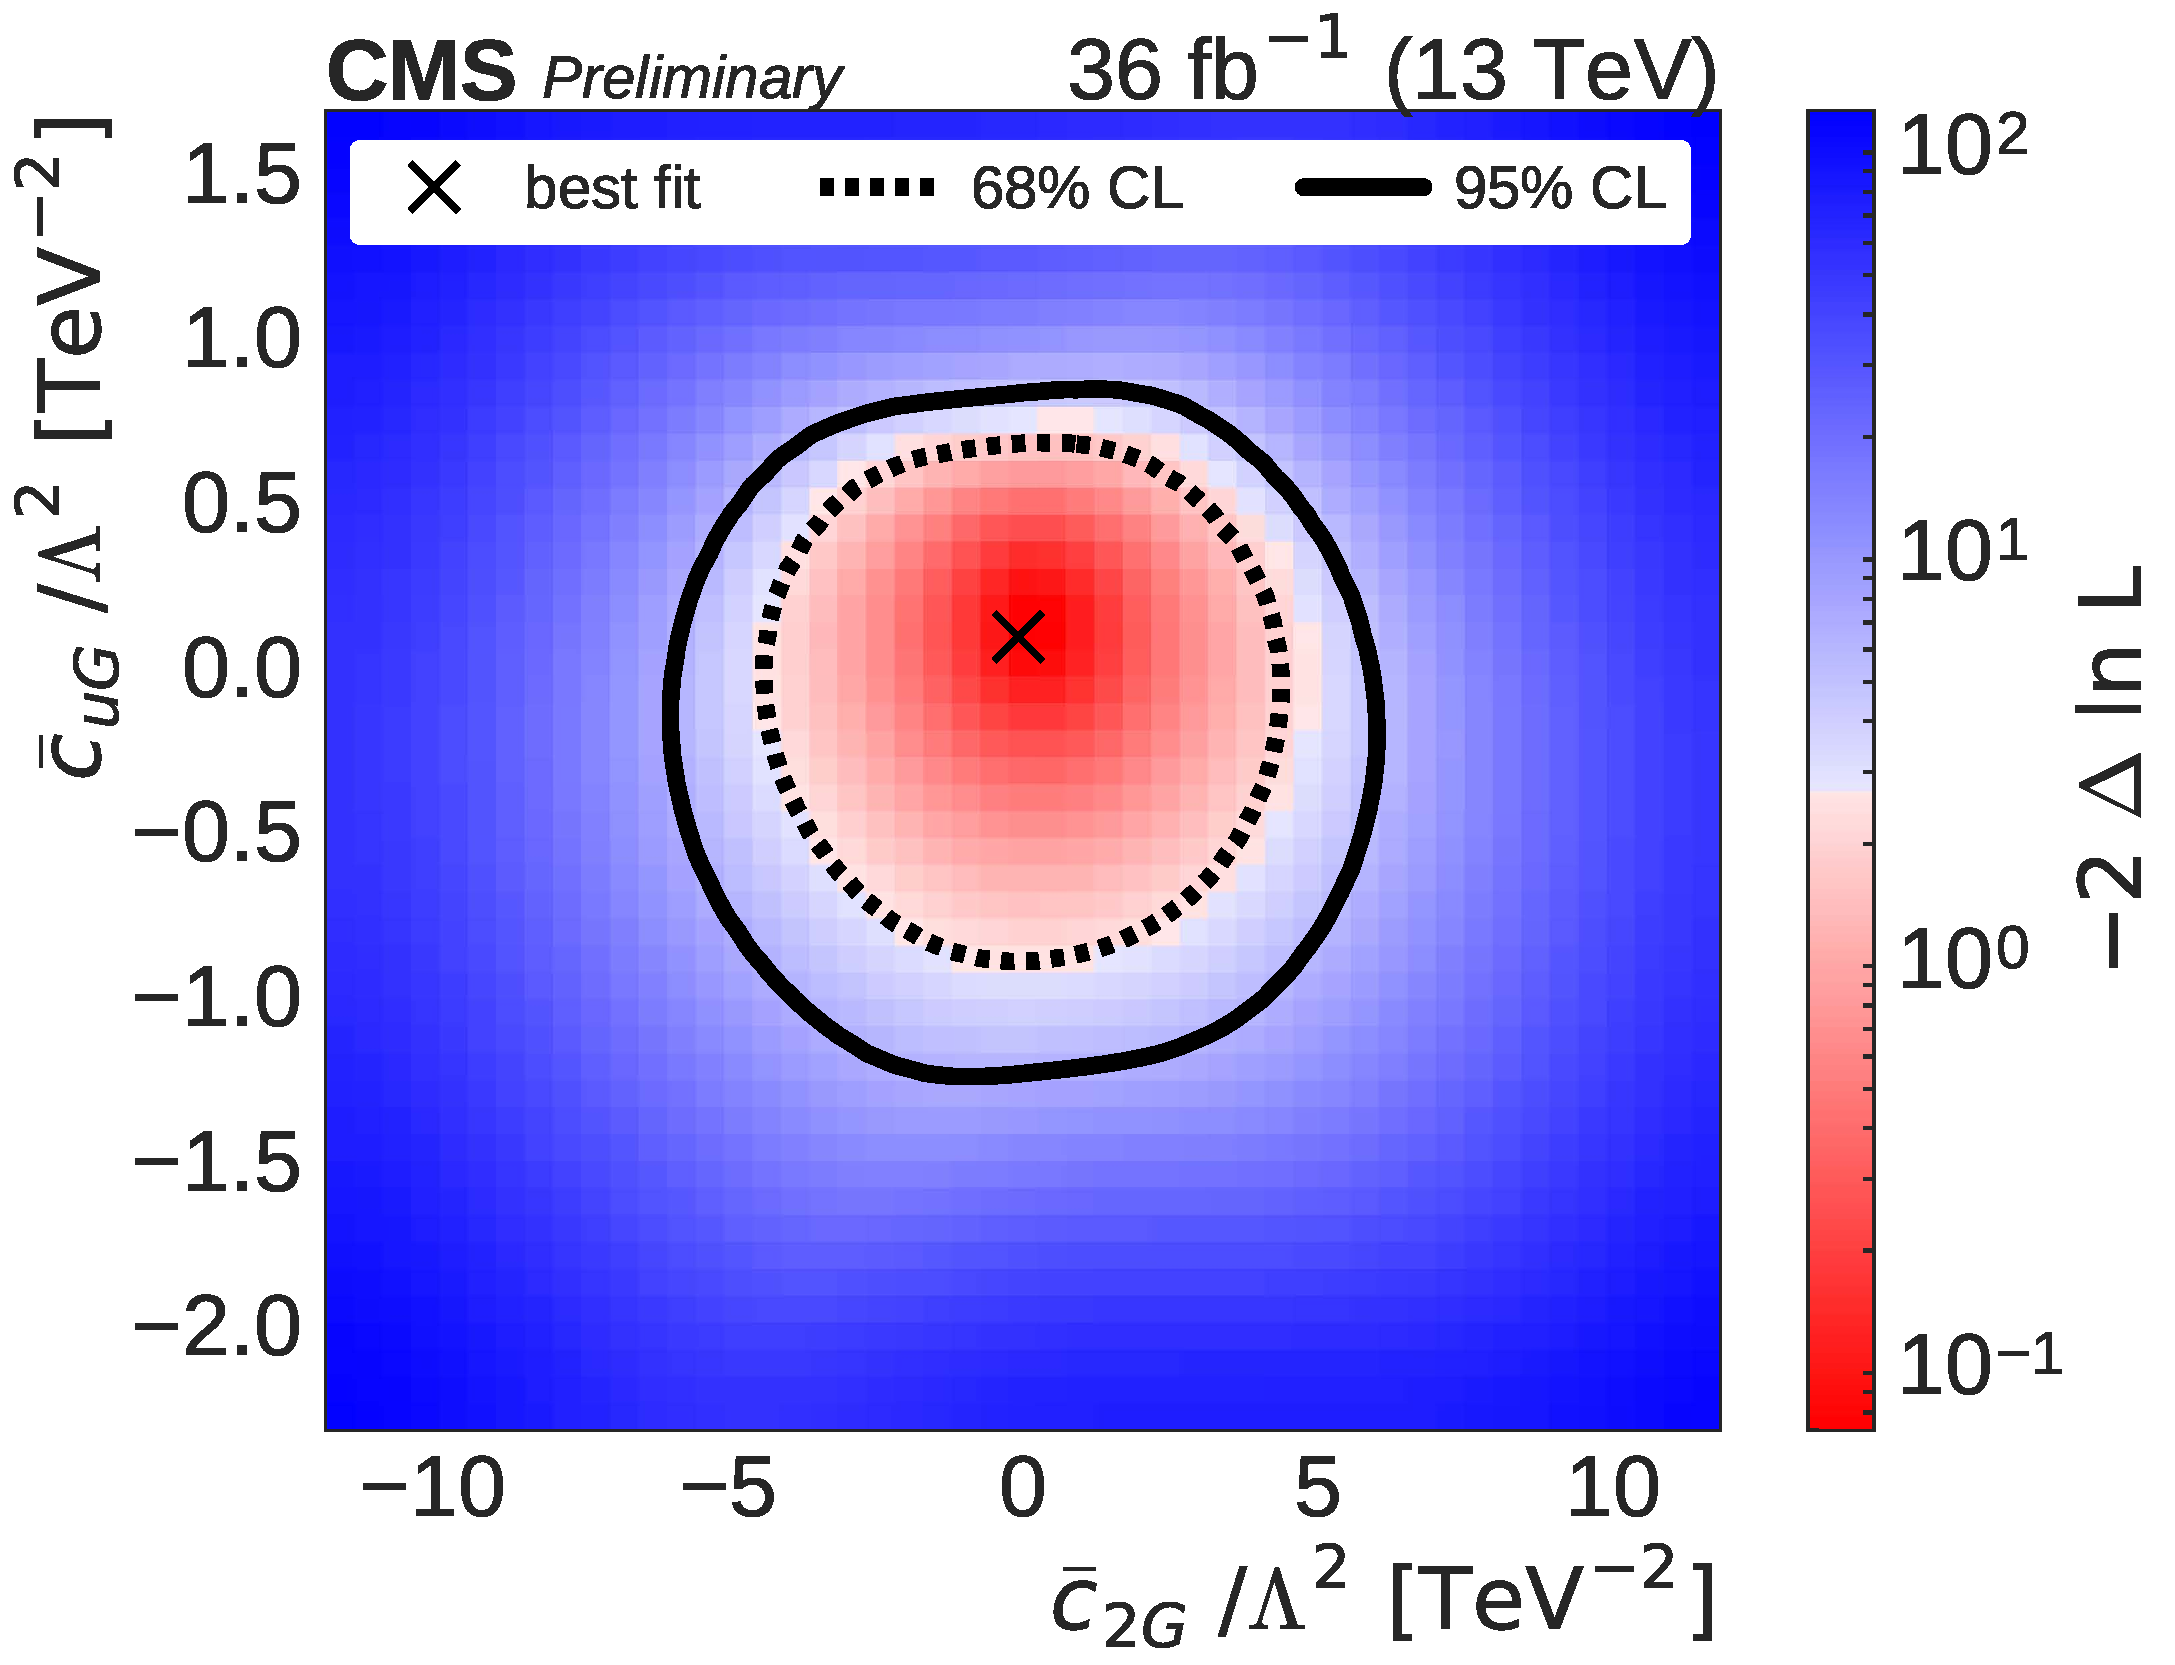
\includegraphics[width=0.6\linewidth]{figures/thirteen-TeV/nll/c2G_cuG}
    \caption{}
  \end{subfigure}
  \vspace{-1cm}
  \setlength{\capwidth}{15cm}
  \setlength{\capwidth}{15cm}
  \caption[Signal scaling and profile likelihood scan in the \cuG, \ctwoG plane]{Signal scaling
    shown in the \cuG, \ctwoG plane with all other coefficients fixed to zero (a) or their best-fit
    values (b) for \ttZ (left), \ttH (center), and \ttW (right). The color represents the scaling
    ($\sigma_\text{NP + SM} / \sigma_\text{SM}$) due to NP effects. The star represents the SM point in
    which all $c_i=0$. The negative log likelihood is shown in (c). The best fit is represented by a
    cross. The \SI{68}{\percent} and \SI{95}{\percent} CL contours are shown with dashed and solid
  lines, respectively.}
\end{figure}

\begin{figure}
  \vspace{-1cm}
  \begin{subfigure}{\linewidth}
    \centering
    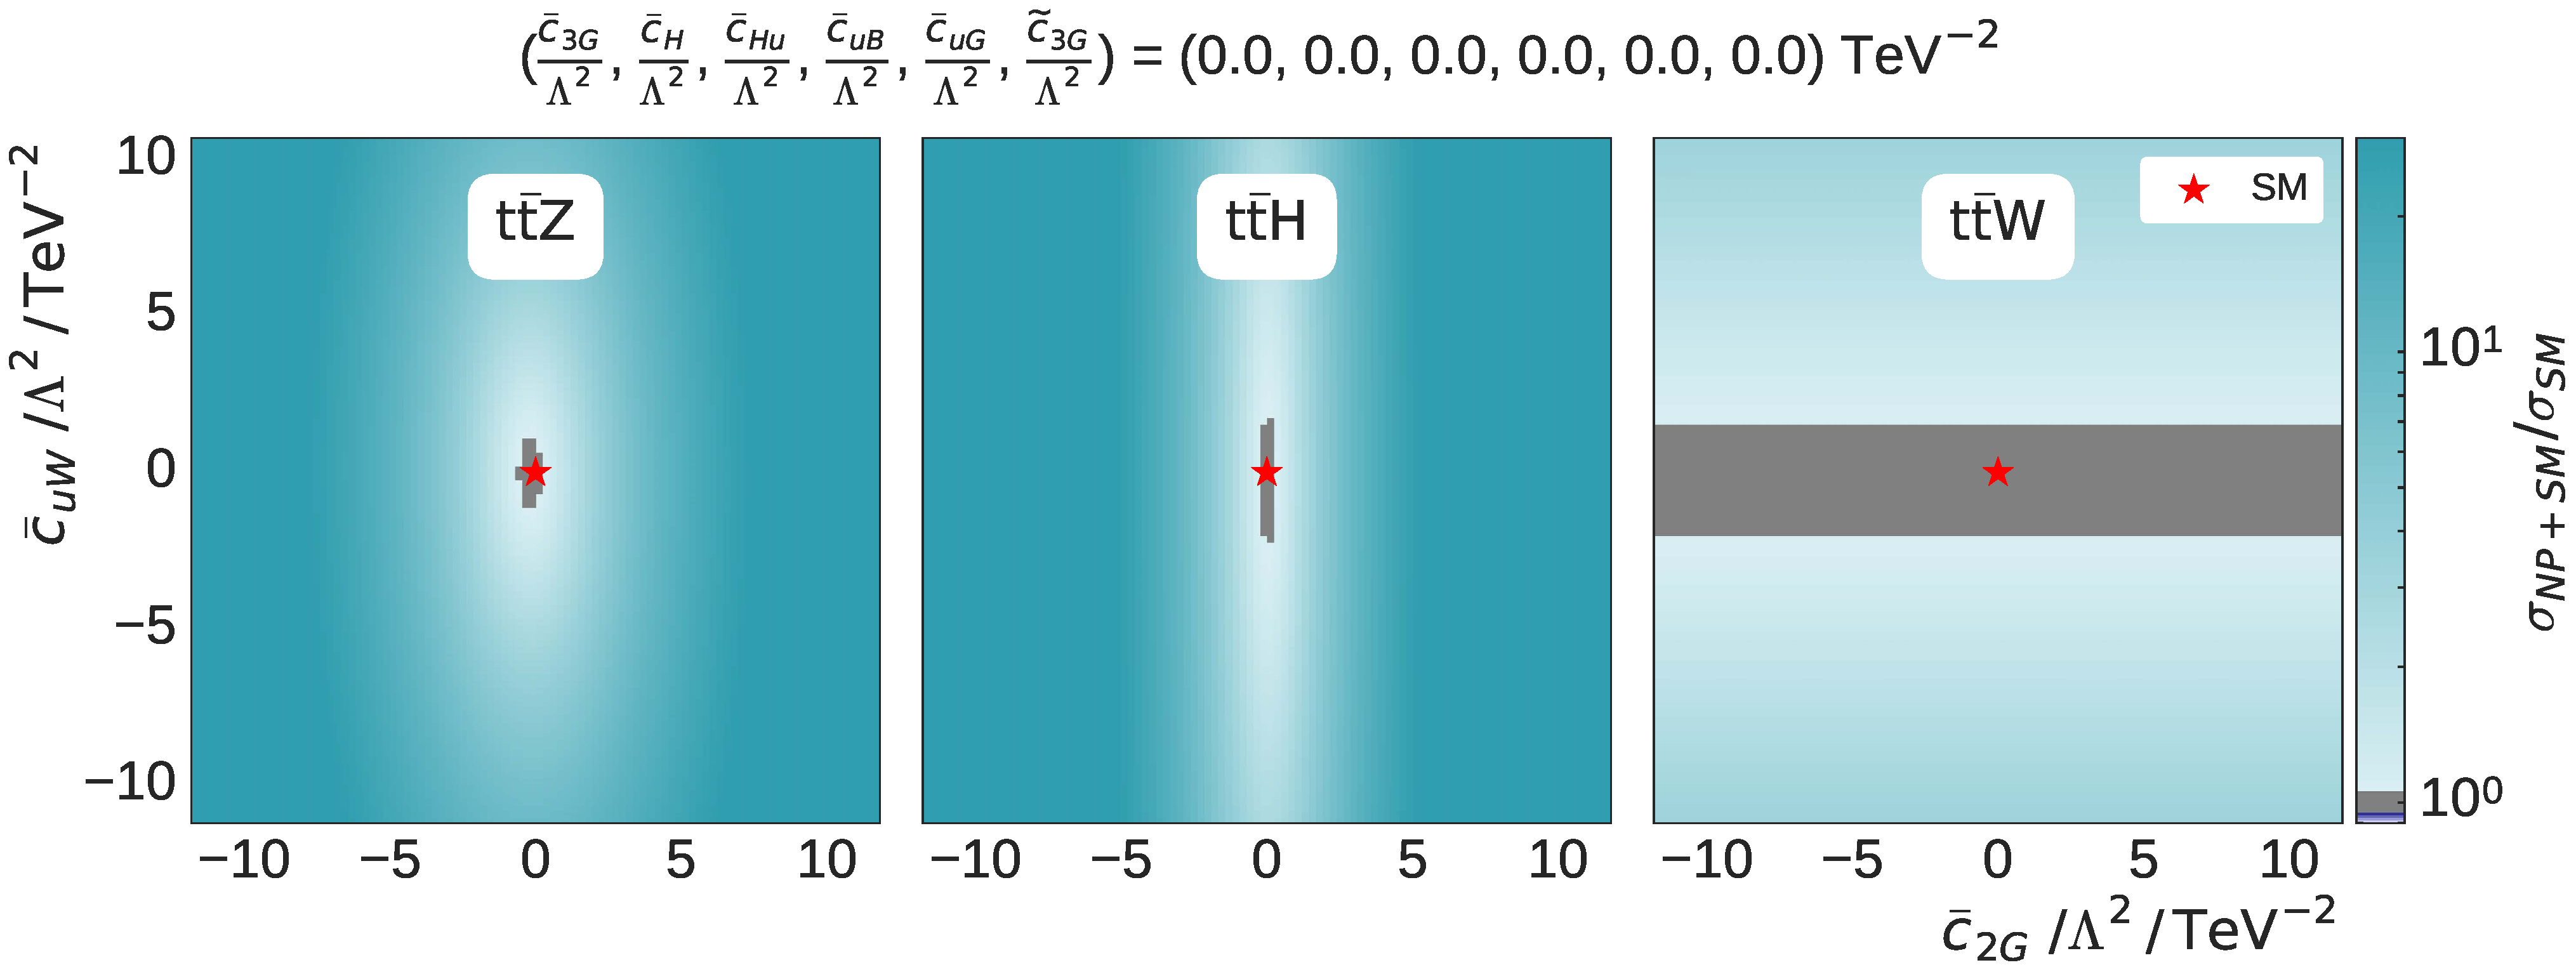
\includegraphics[width=\linewidth]{figures/thirteen-TeV/scaling-frozen/c2G_cuW}
    \caption{}
  \end{subfigure}
  \begin{subfigure}{\linewidth}
    \centering
    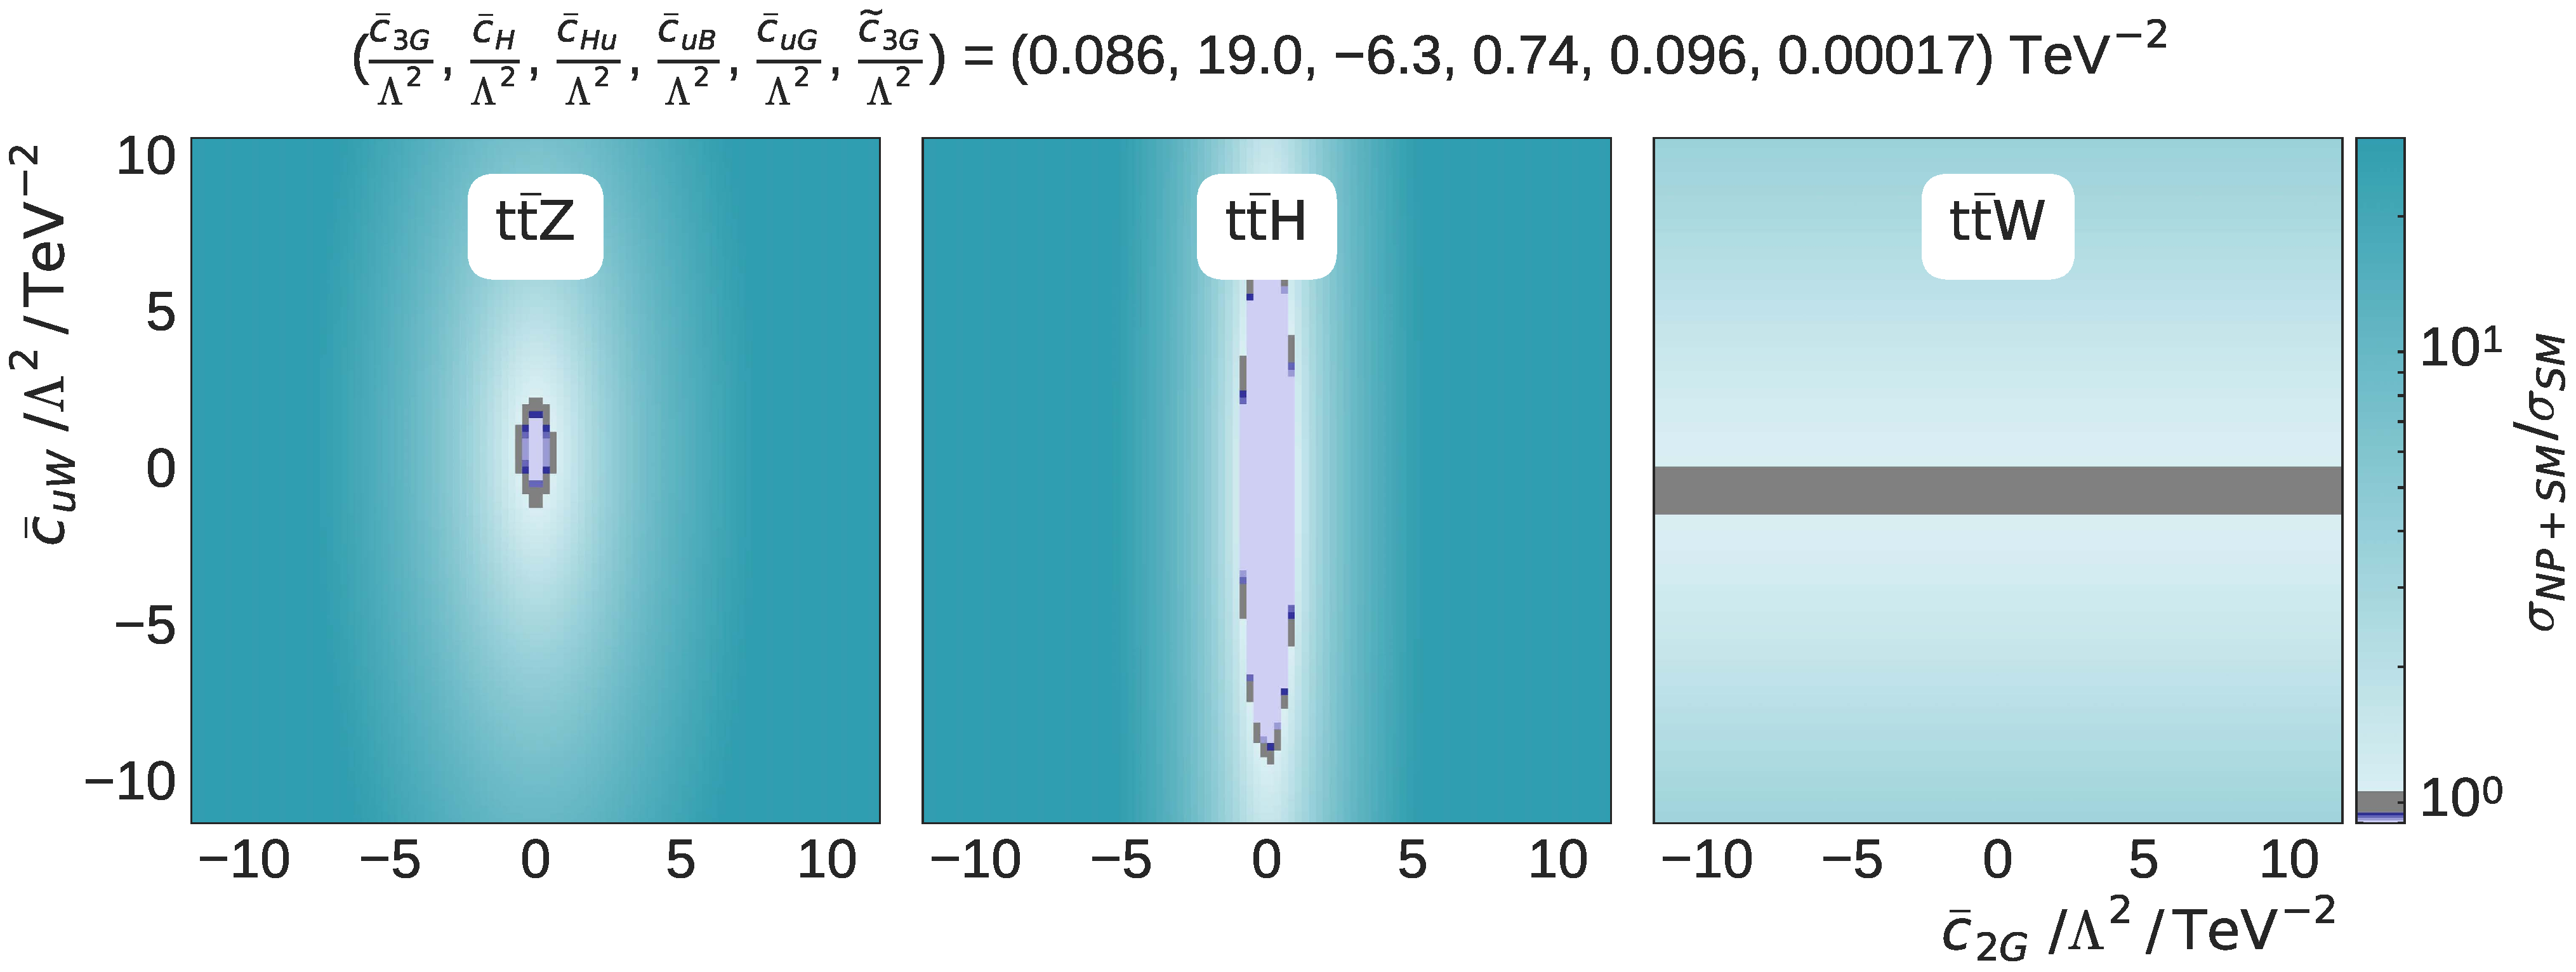
\includegraphics[width=\linewidth]{figures/thirteen-TeV/scaling/c2G_cuW}
    \caption{}
  \end{subfigure}
  \begin{subfigure}{\linewidth}
    \centering
    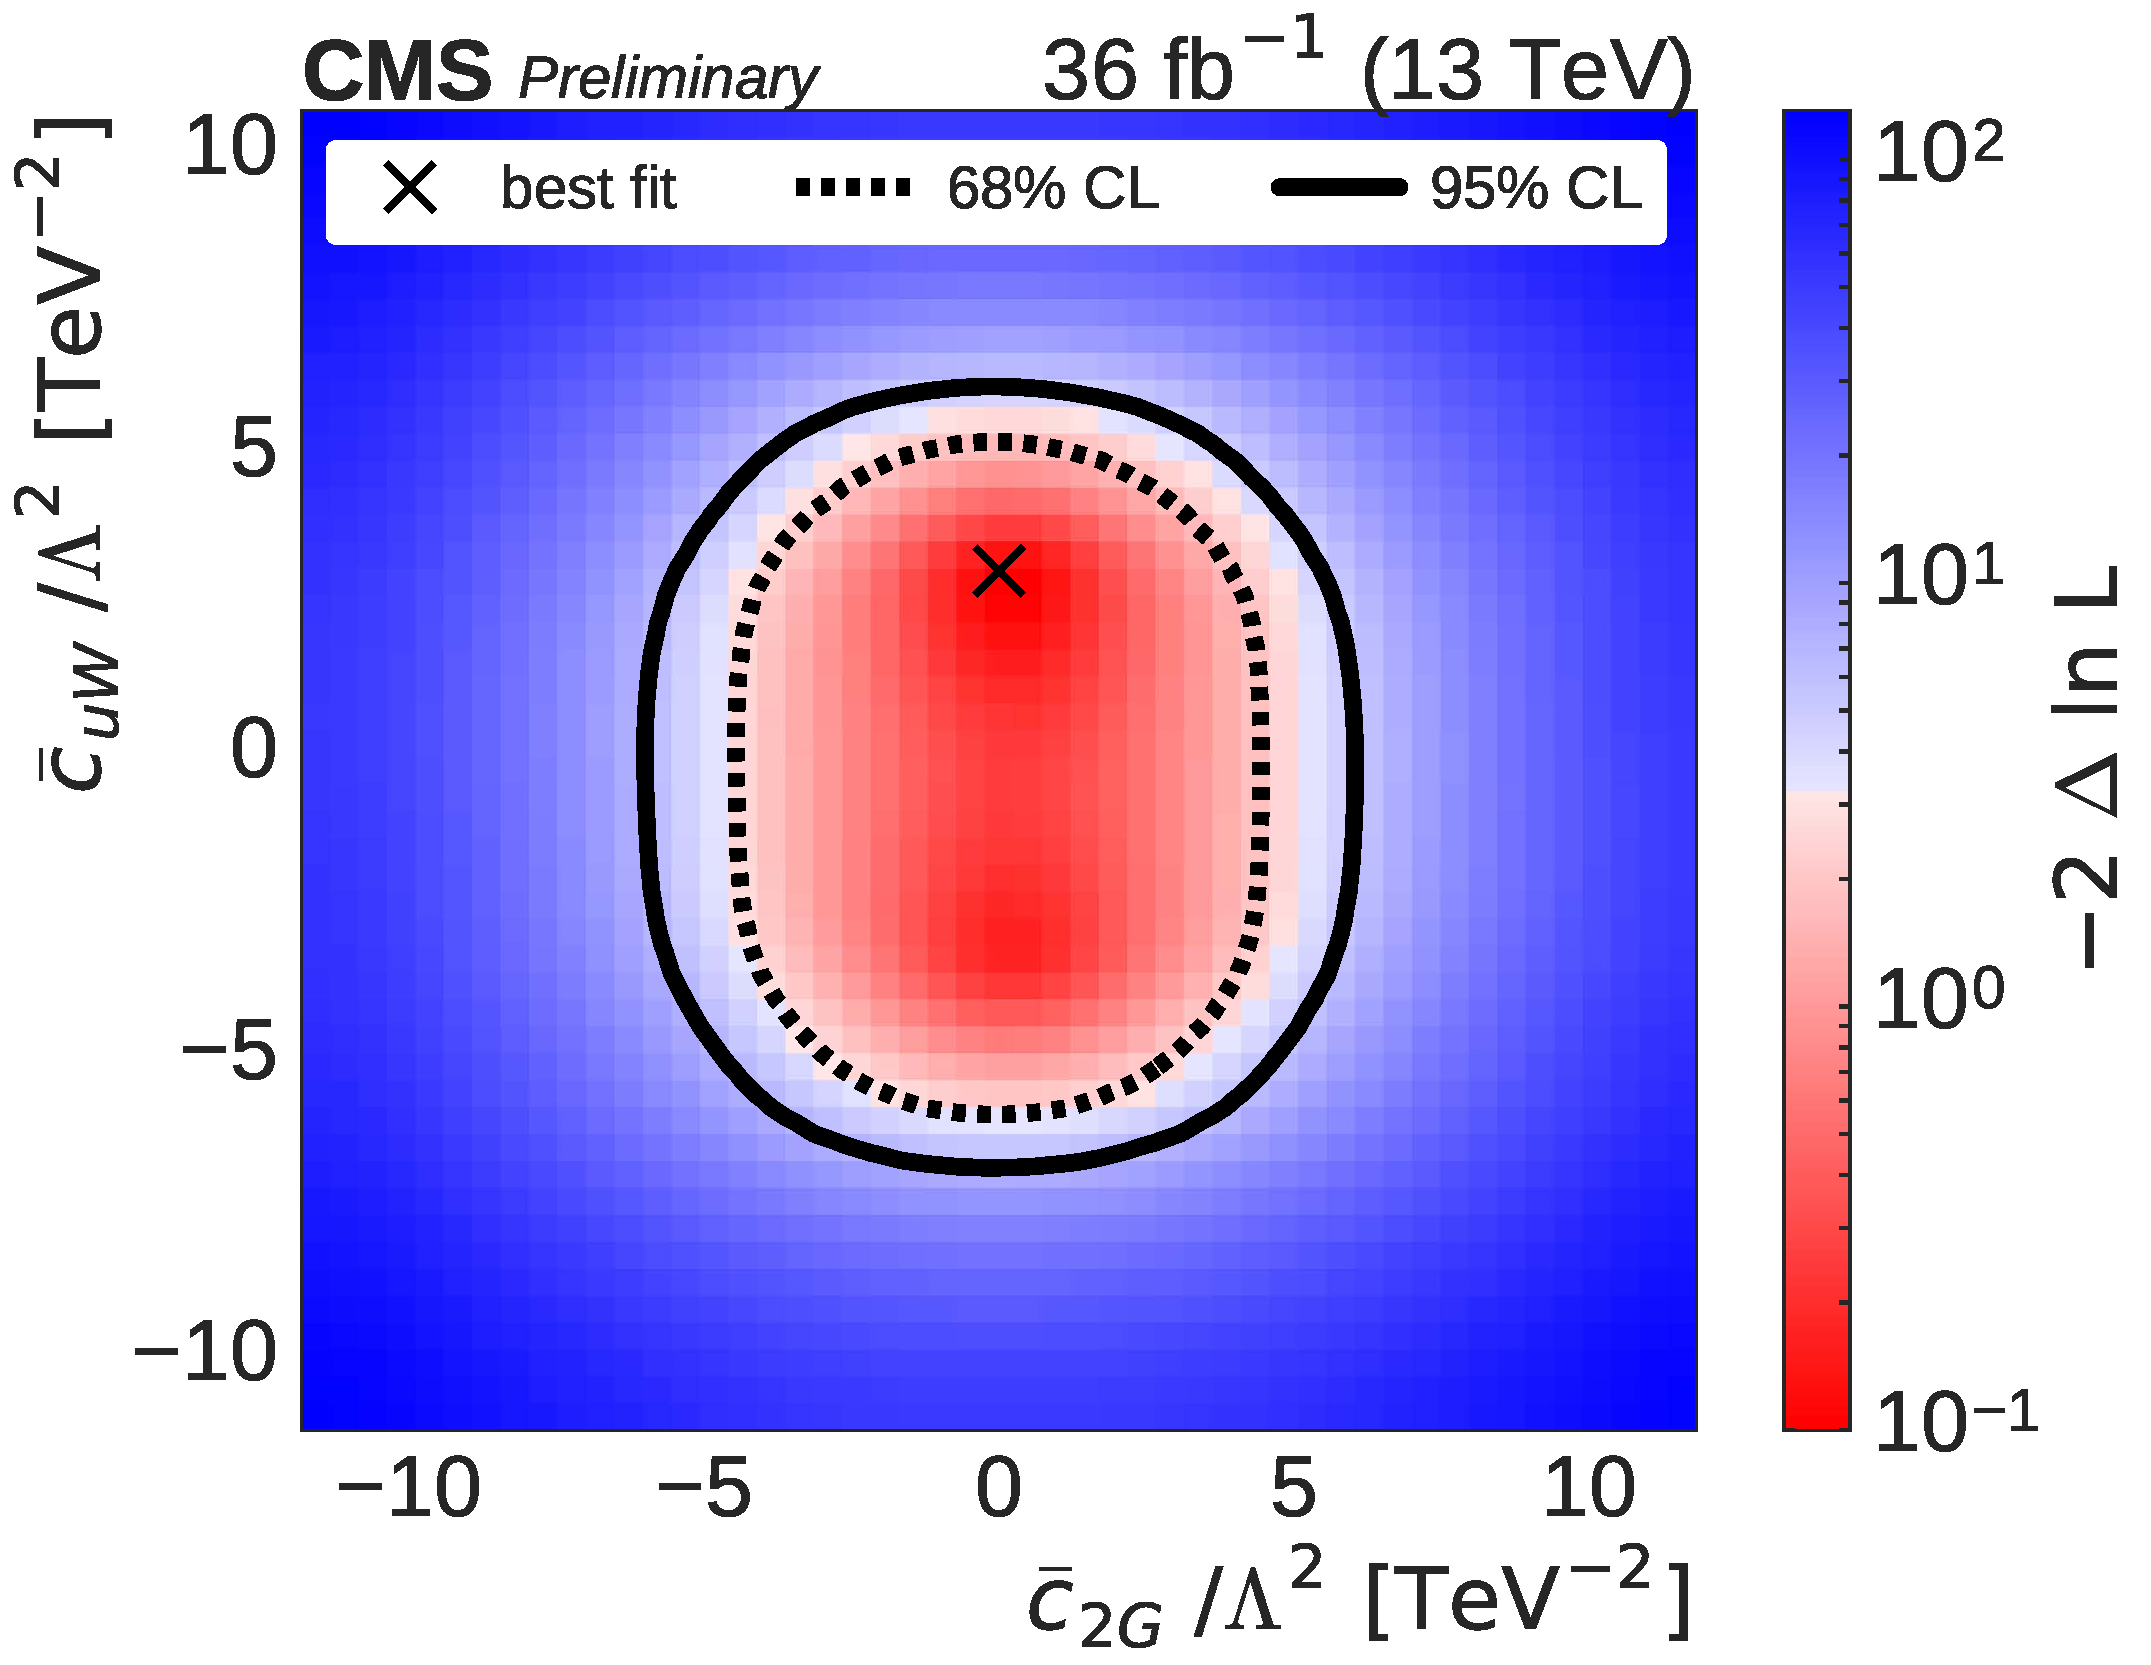
\includegraphics[width=0.6\linewidth]{figures/thirteen-TeV/nll/c2G_cuW}
    \caption{}
  \end{subfigure}
  \vspace{-1cm}
  \setlength{\capwidth}{15cm}
  \caption[Signal scaling and profile likelihood scan in the \cuW, \ctwoG plane]{Signal scaling
  shown in the \cuW, \ctwoG plane with all other coefficients fixed to zero (a) or their best-fit
  values (b) for \ttZ (left), \ttH (center), and \ttW (right). The color represents the scaling
  ($\sigma_\text{NP + SM} / \sigma_\text{SM}$) due to NP effects. The star represents the SM point in
  which all $c_i=0$. The negative log likelihood is shown in (c). The best fit is represented by a
  cross. The \SI{68}{\percent} and \SI{95}{\percent} CL contours are shown with dashed and solid
  lines, respectively.}
\end{figure}

\begin{figure}
  \vspace{-1cm}
  \begin{subfigure}{\linewidth}
    \centering
    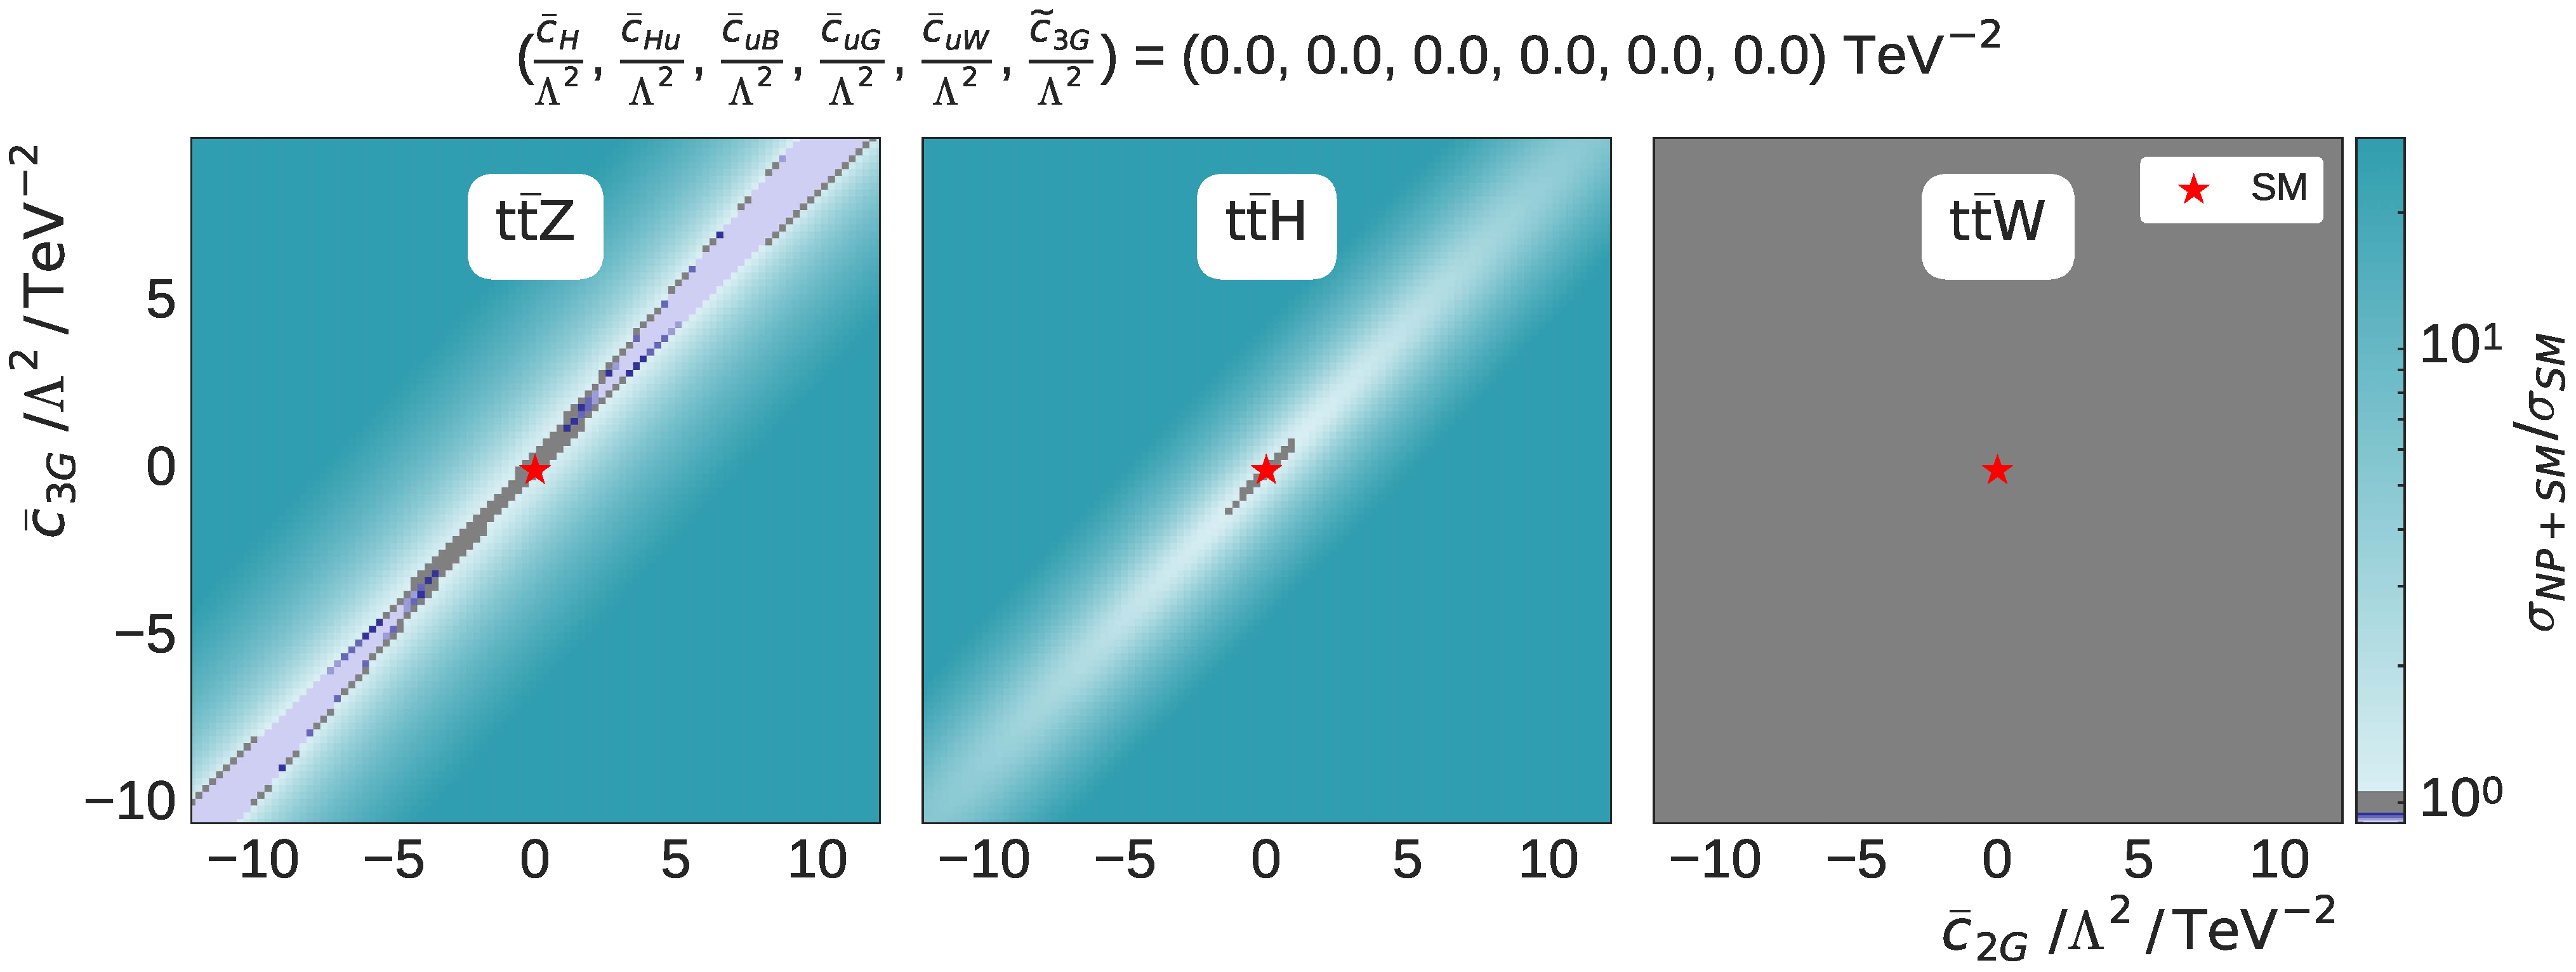
\includegraphics[width=\linewidth]{figures/thirteen-TeV/scaling-frozen/c2G_c3G}
    \caption{}
  \end{subfigure}
  \begin{subfigure}{\linewidth}
    \centering
    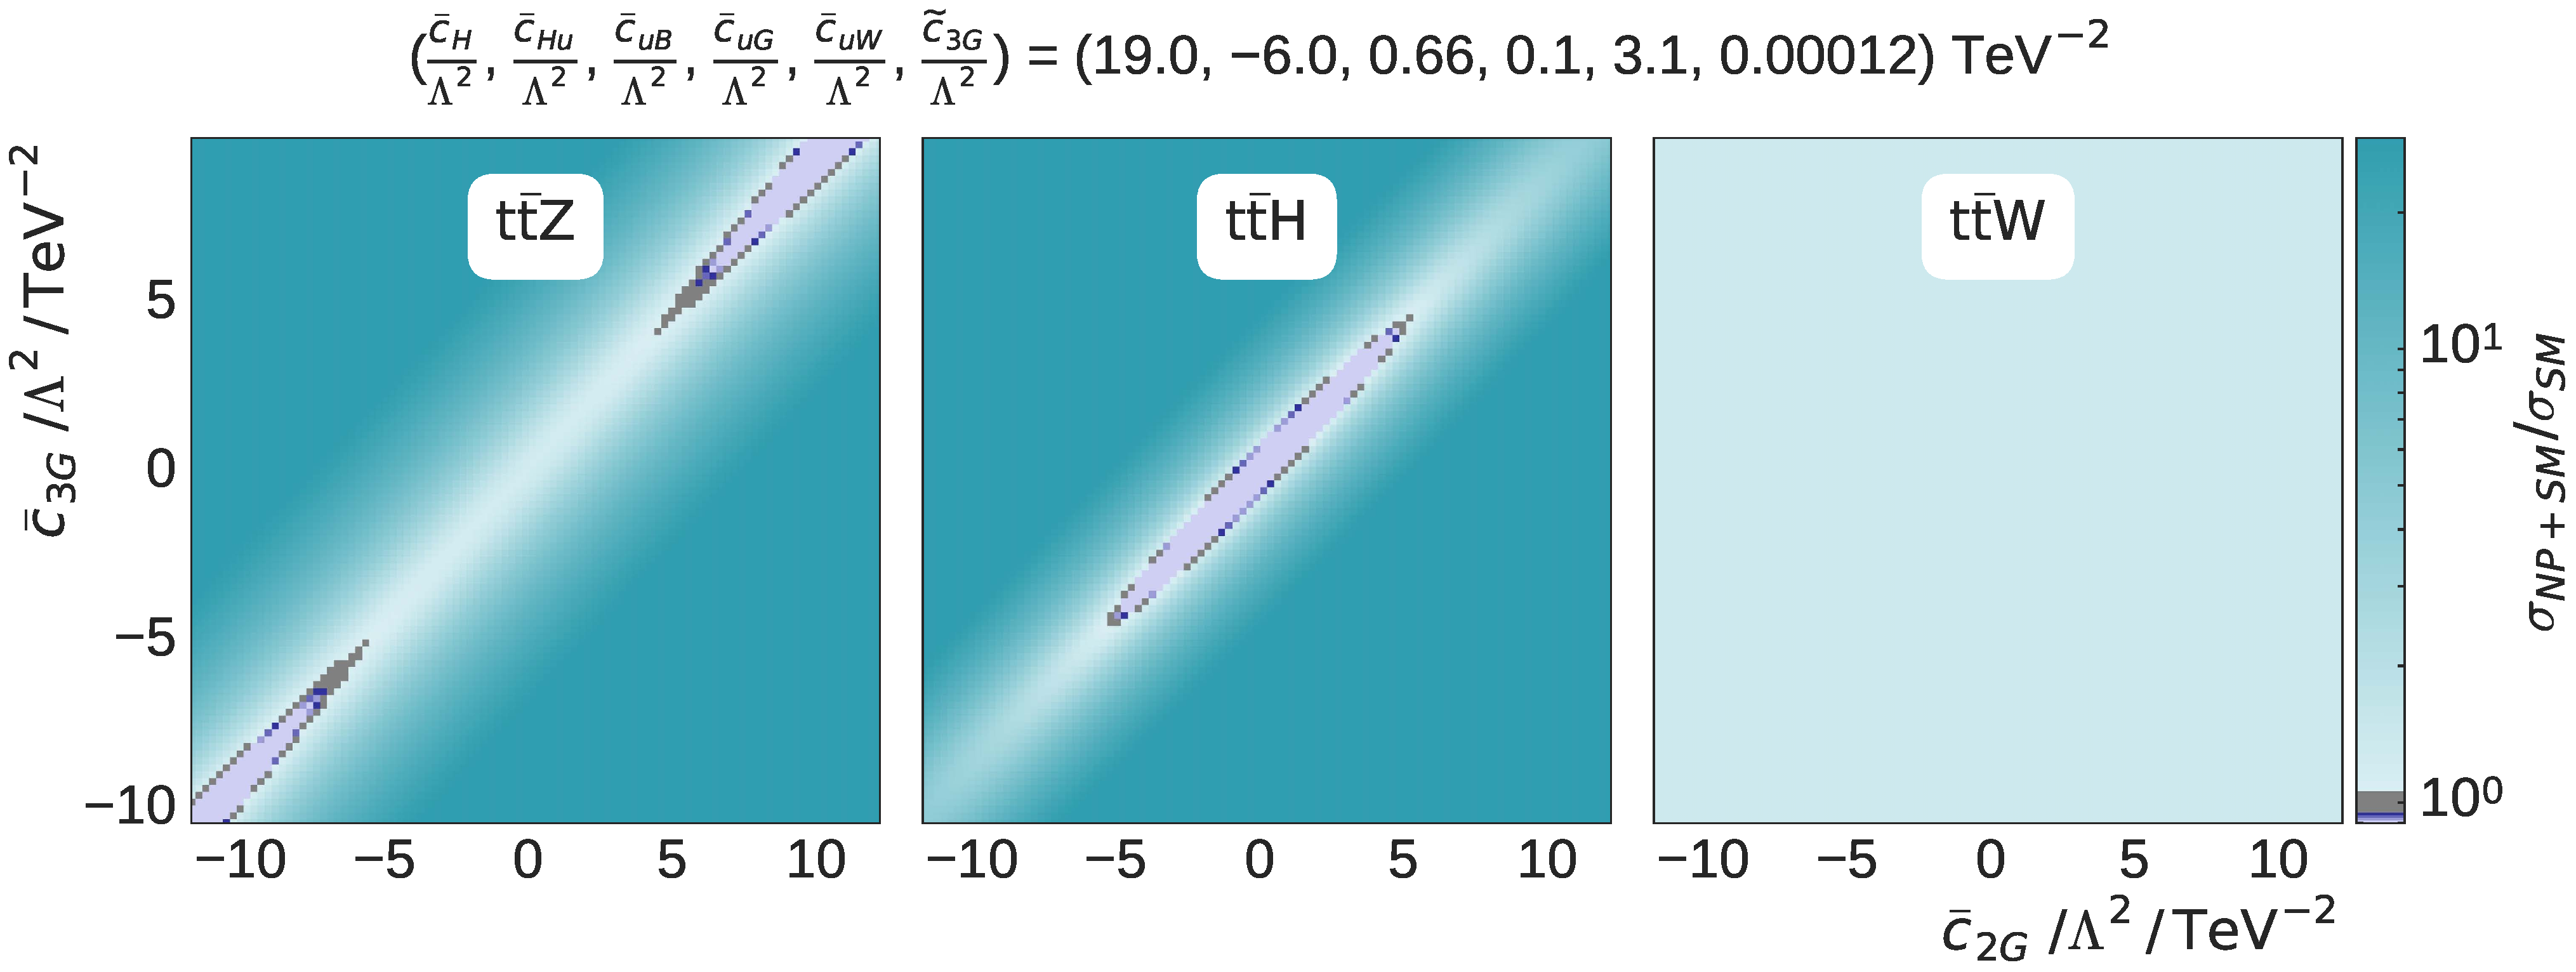
\includegraphics[width=\linewidth]{figures/thirteen-TeV/scaling/c2G_c3G}
    \caption{}
  \end{subfigure}
  \begin{subfigure}{\linewidth}
    \centering
    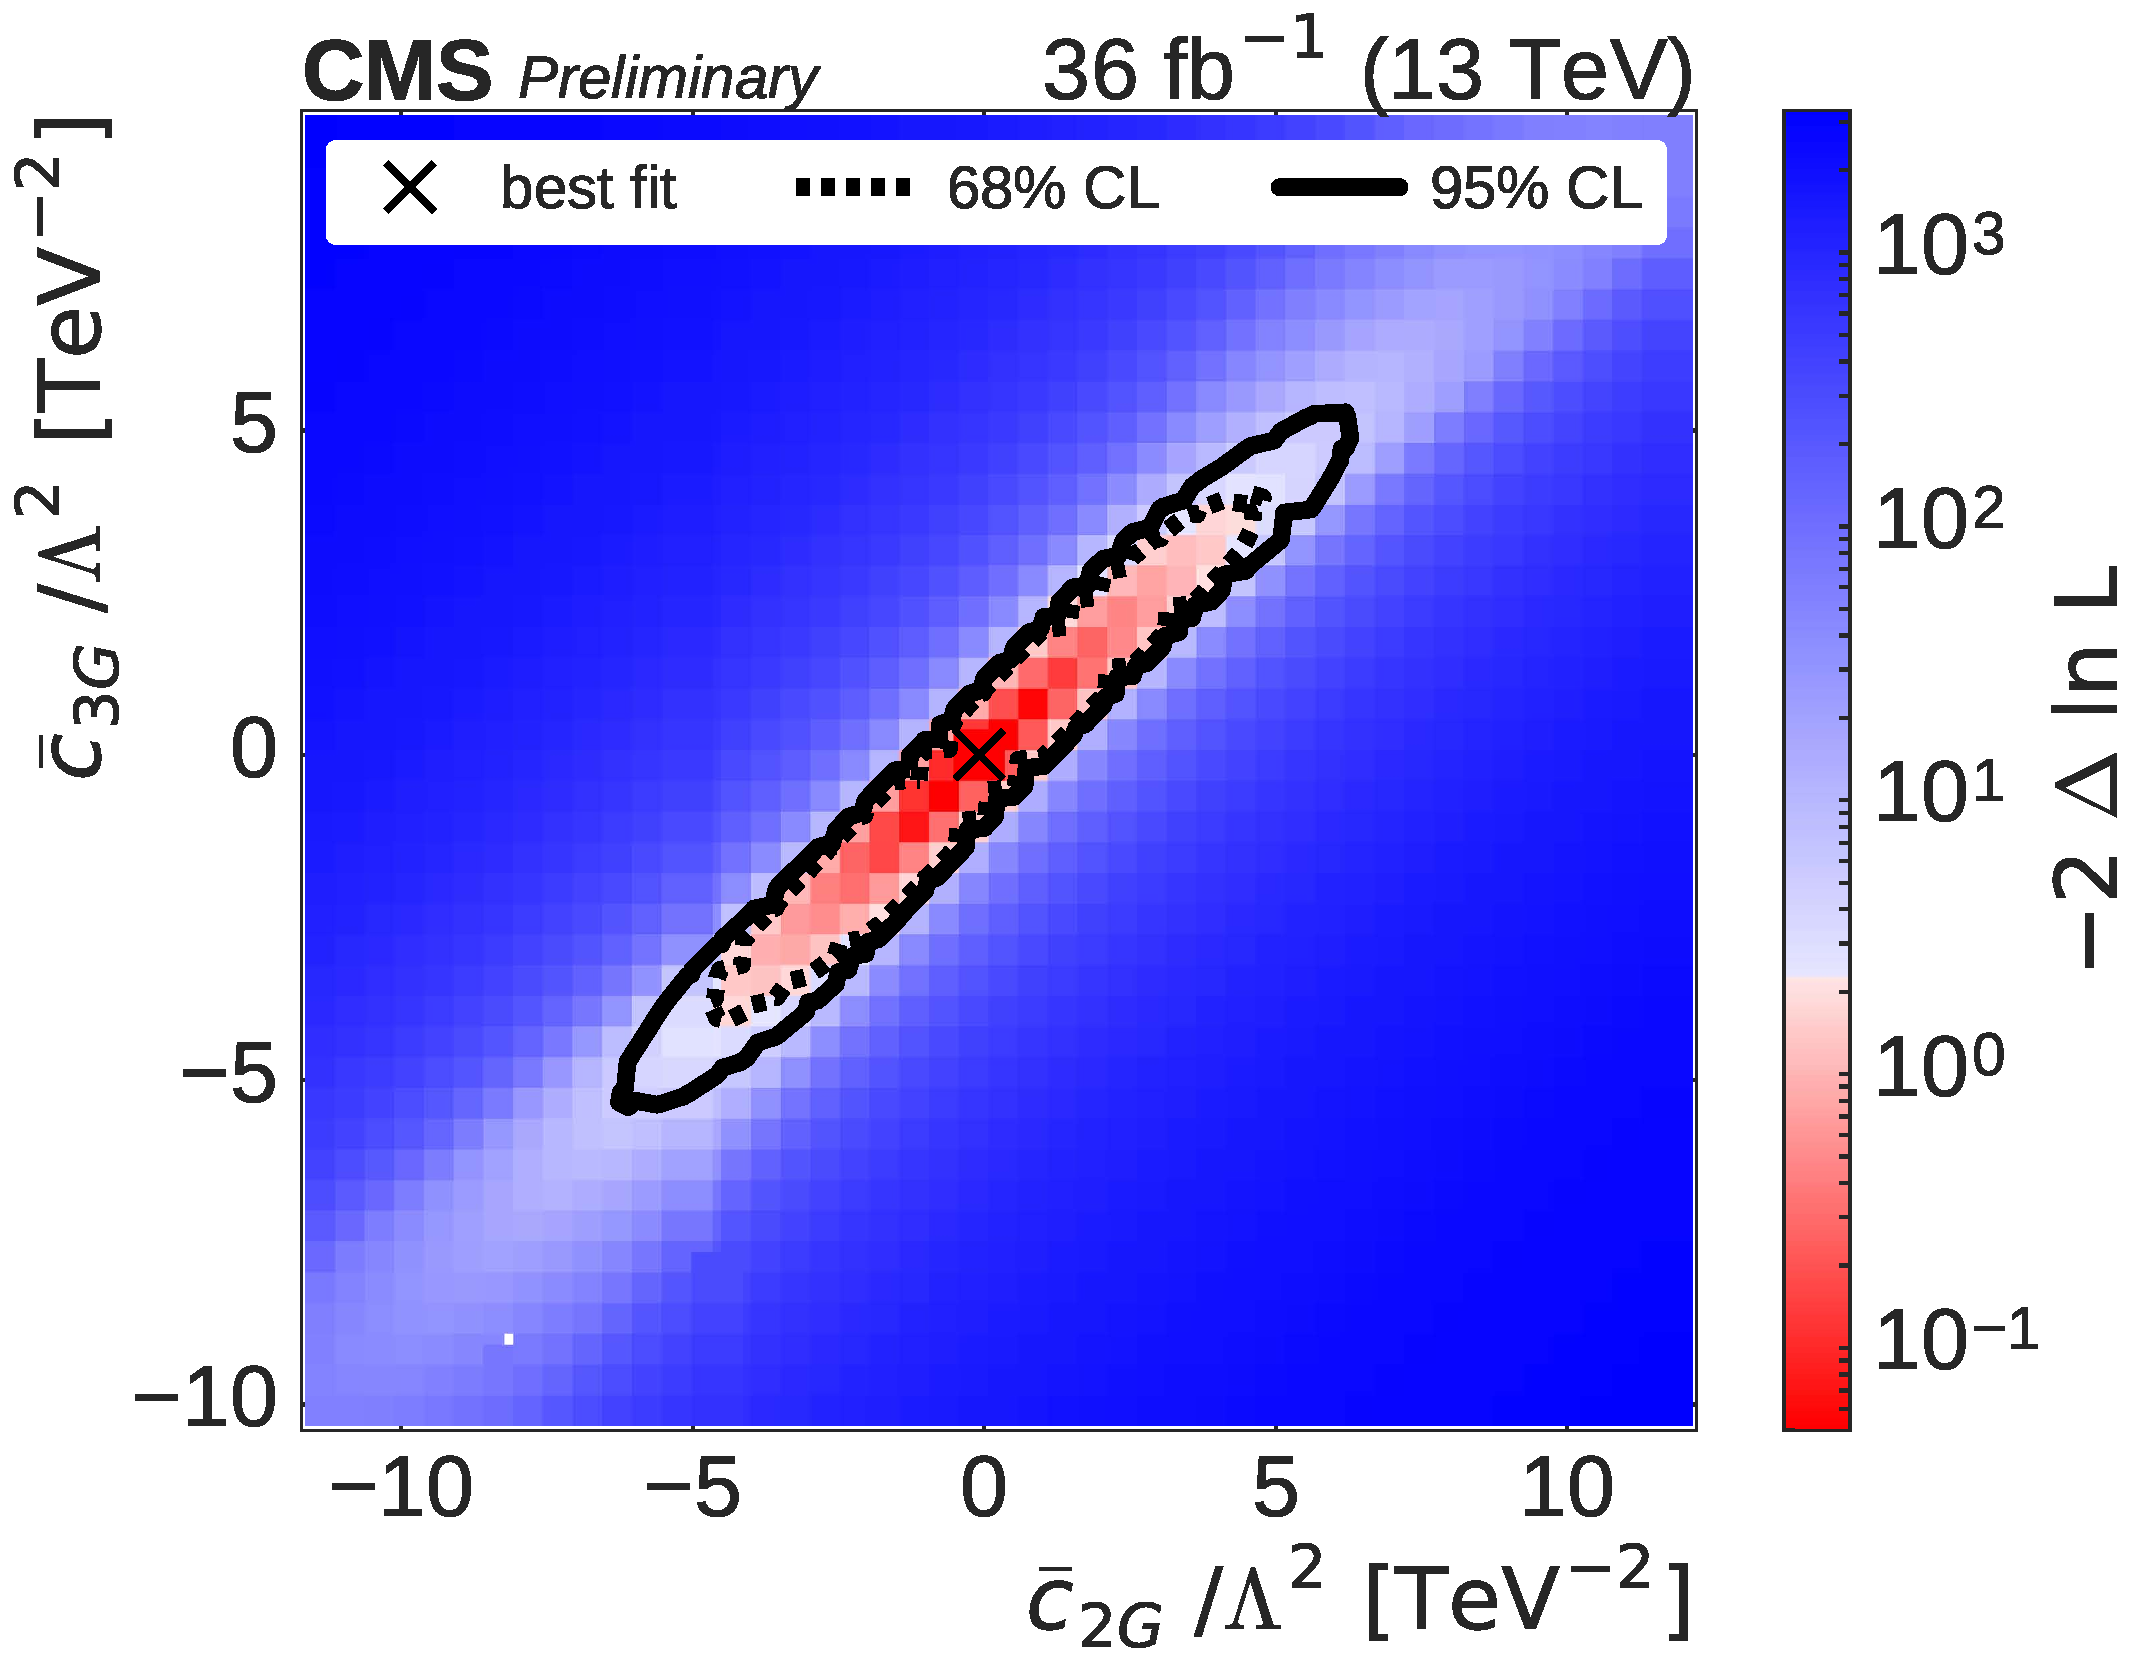
\includegraphics[width=0.6\linewidth]{figures/thirteen-TeV/nll/c2G_c3G}
    \caption{}
  \end{subfigure}
  \vspace{-1cm}
  \setlength{\capwidth}{15cm}
  \caption[Signal scaling and profile likelihood scan in the \cthreeG, \ctwoG plane]{Signal scaling
  shown in the \cthreeG, \ctwoG plane with all other coefficients fixed to zero (a) or their
  best-fit values (b) for \ttZ (left), \ttH (center), and \ttW (right). The color represents the
  scaling ($\sigma_\text{NP + SM} / \sigma_\text{SM}$) due to NP effects. The star represents the SM
  point in which all $c_i=0$. The negative log likelihood is shown in (c). The best fit is represented
  by a cross. The \SI{68}{\percent} and \SI{95}{\percent} CL contours are shown with dashed and solid
  lines, respectively.}
\end{figure}

\begin{figure}
  \vspace{-1cm}
  \begin{subfigure}{\linewidth}
    \centering
    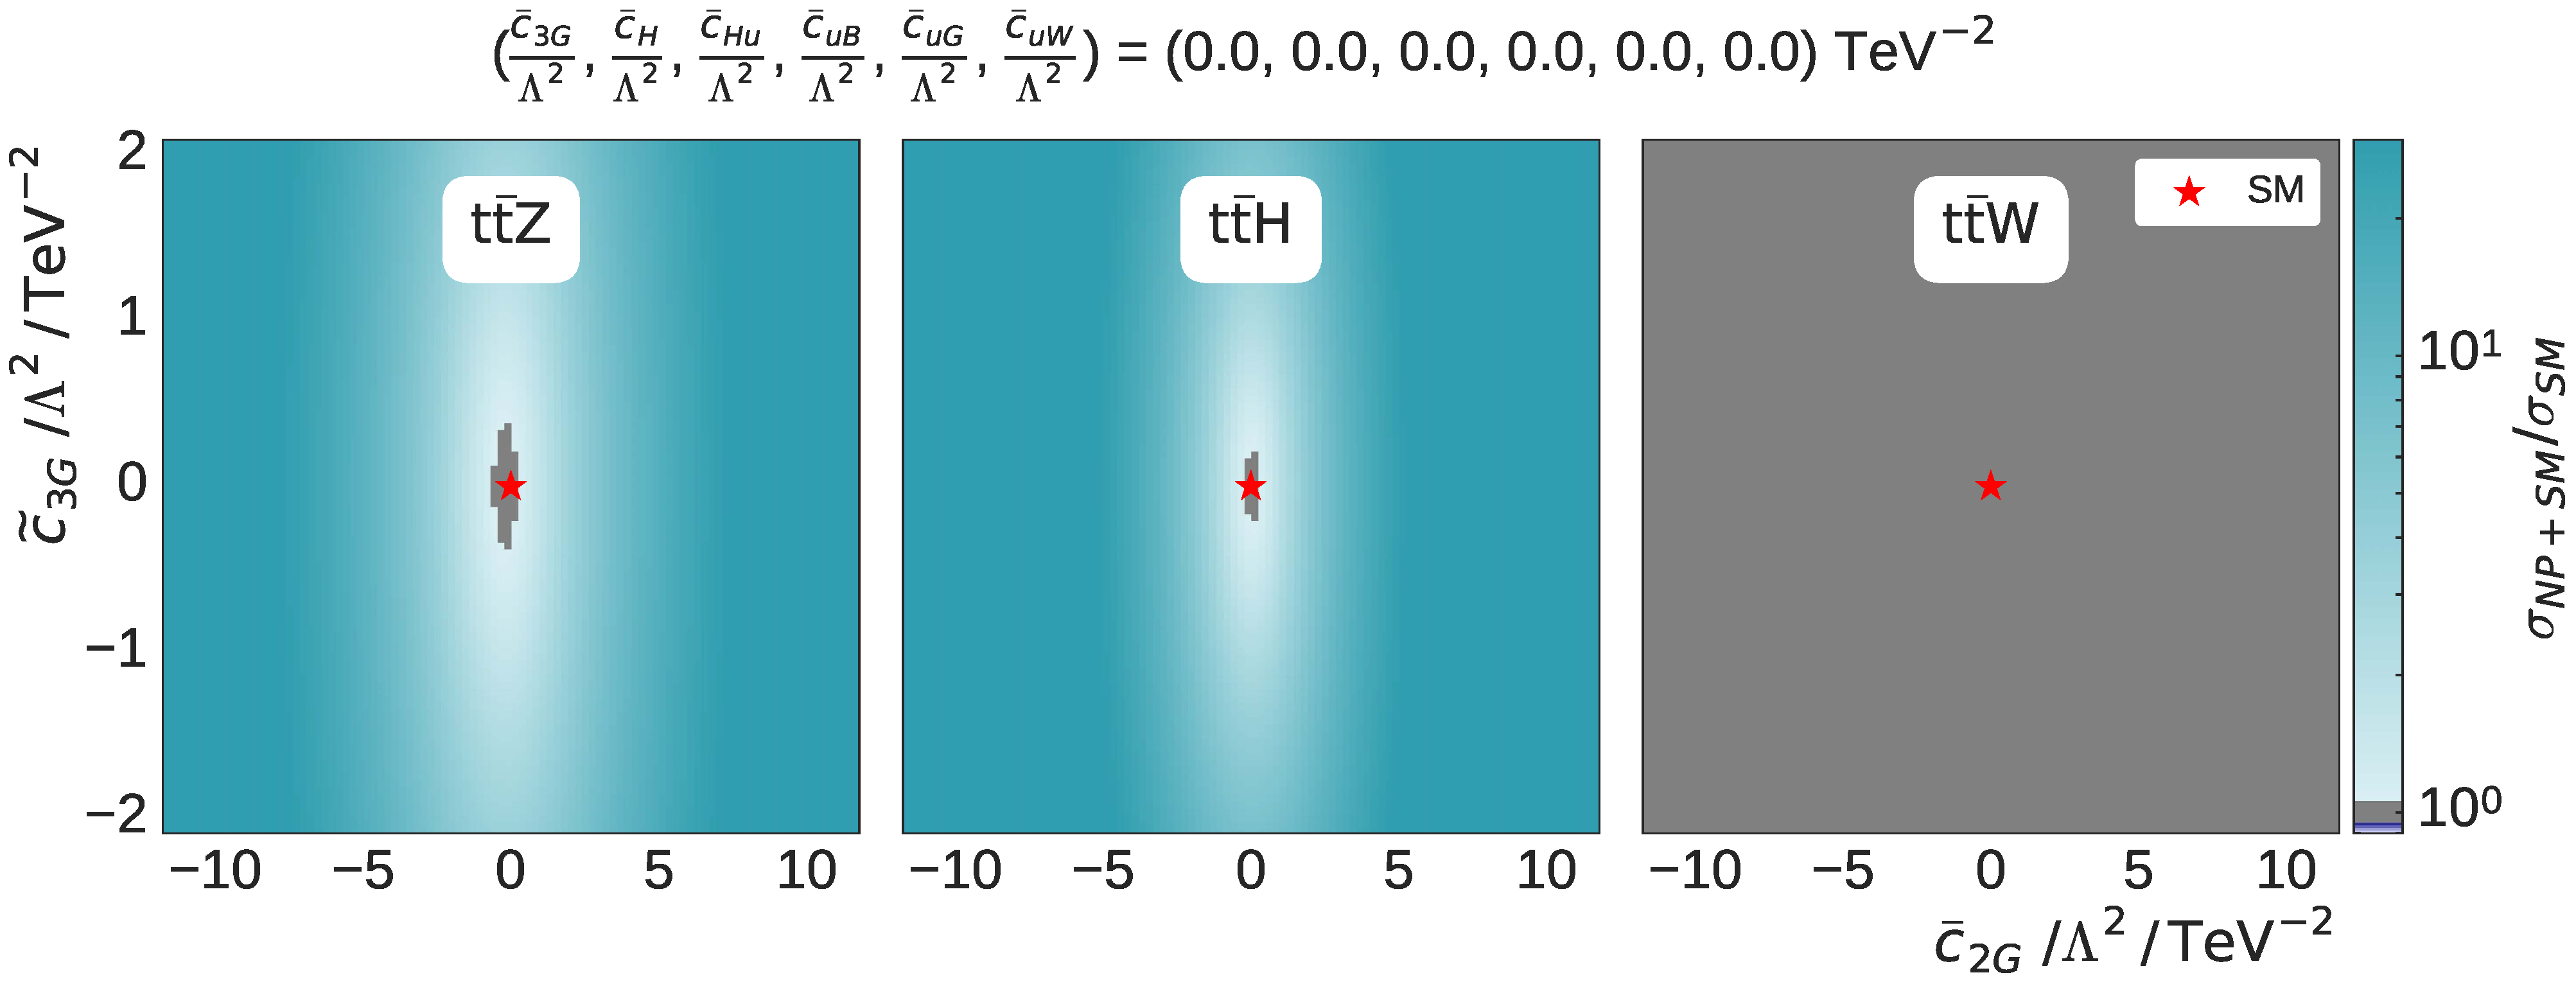
\includegraphics[width=\linewidth]{figures/thirteen-TeV/scaling-frozen/c2G_tc3G}
    \caption{}
  \end{subfigure}
  \begin{subfigure}{\linewidth}
    \centering
    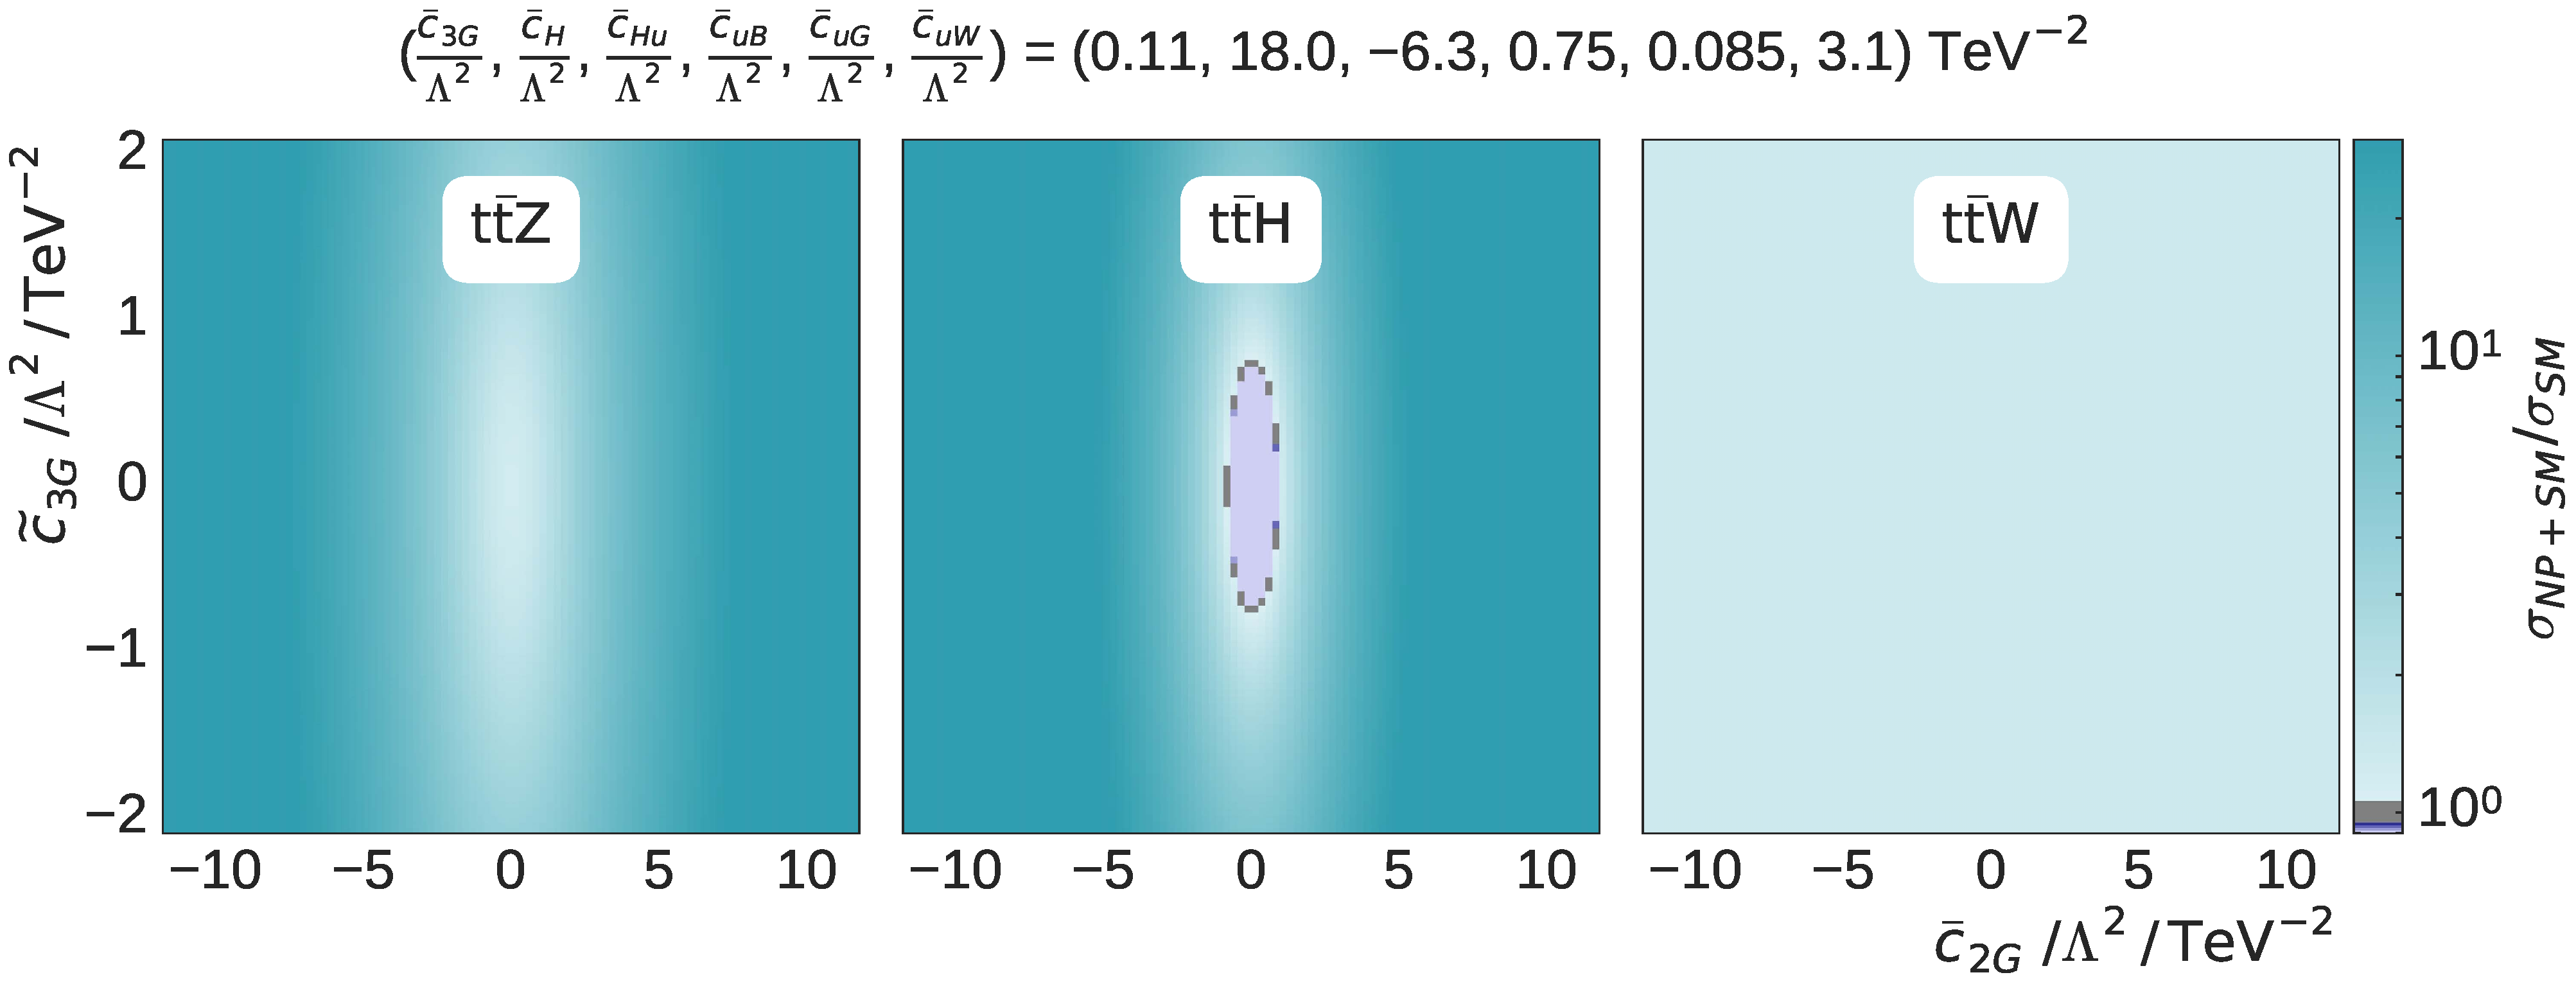
\includegraphics[width=\linewidth]{figures/thirteen-TeV/scaling/c2G_tc3G}
    \caption{}
  \end{subfigure}
  \begin{subfigure}{\linewidth}
    \centering
    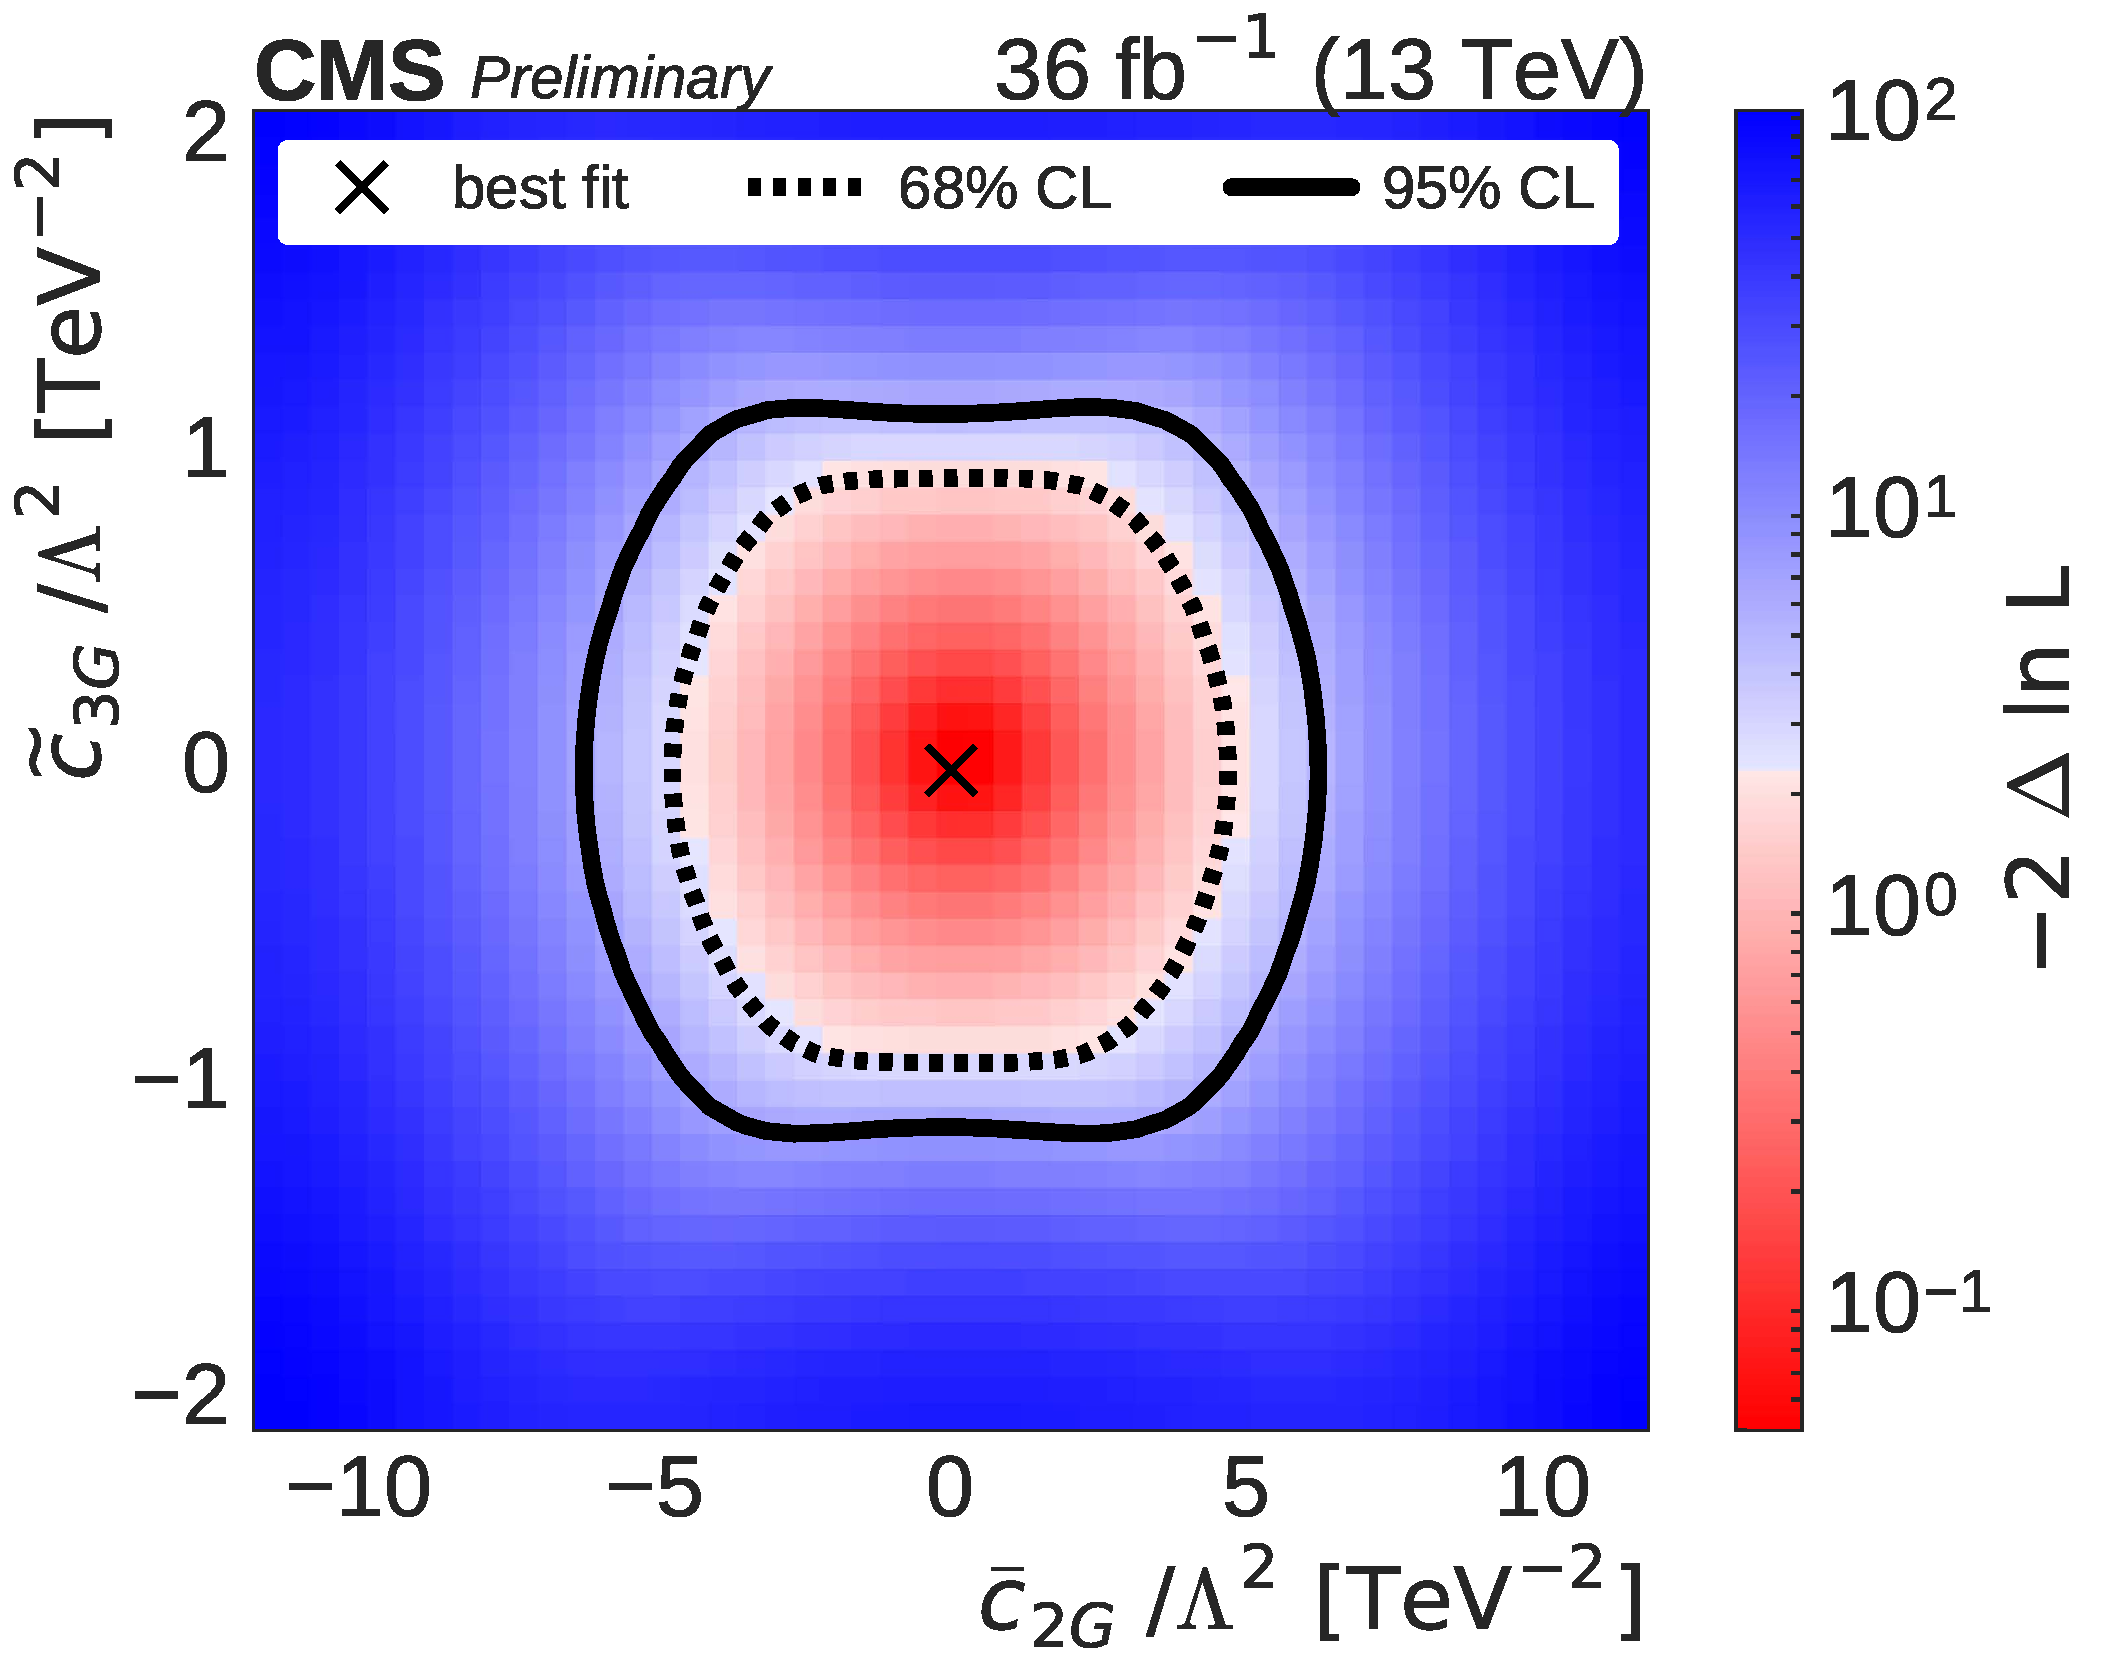
\includegraphics[width=0.6\linewidth]{figures/thirteen-TeV/nll/c2G_tc3G}
    \caption{}
  \end{subfigure}
  \vspace{-1cm}
  \setlength{\capwidth}{15cm}
  \caption[Signal scaling and profile likelihood scan in the \tcthreeG, \ctwoG plane]{Signal scaling
  shown in the \tcthreeG, \ctwoG plane with all other coefficients fixed to zero (a) or their
  best-fit values (b) for \ttZ (left), \ttH (center), and \ttW (right). The color represents the
  scaling ($\sigma_\text{NP + SM} / \sigma_\text{SM}$) due to NP effects. The star represents the SM
  point in which all $c_i=0$. The negative log likelihood is shown in (c). The best fit is represented
  by a cross. The \SI{68}{\percent} and \SI{95}{\percent} CL contours are shown with dashed and solid
  lines, respectively.}
\end{figure}

\begin{figure}
  \vspace{-1cm}
  \begin{subfigure}{\linewidth}
    \centering
    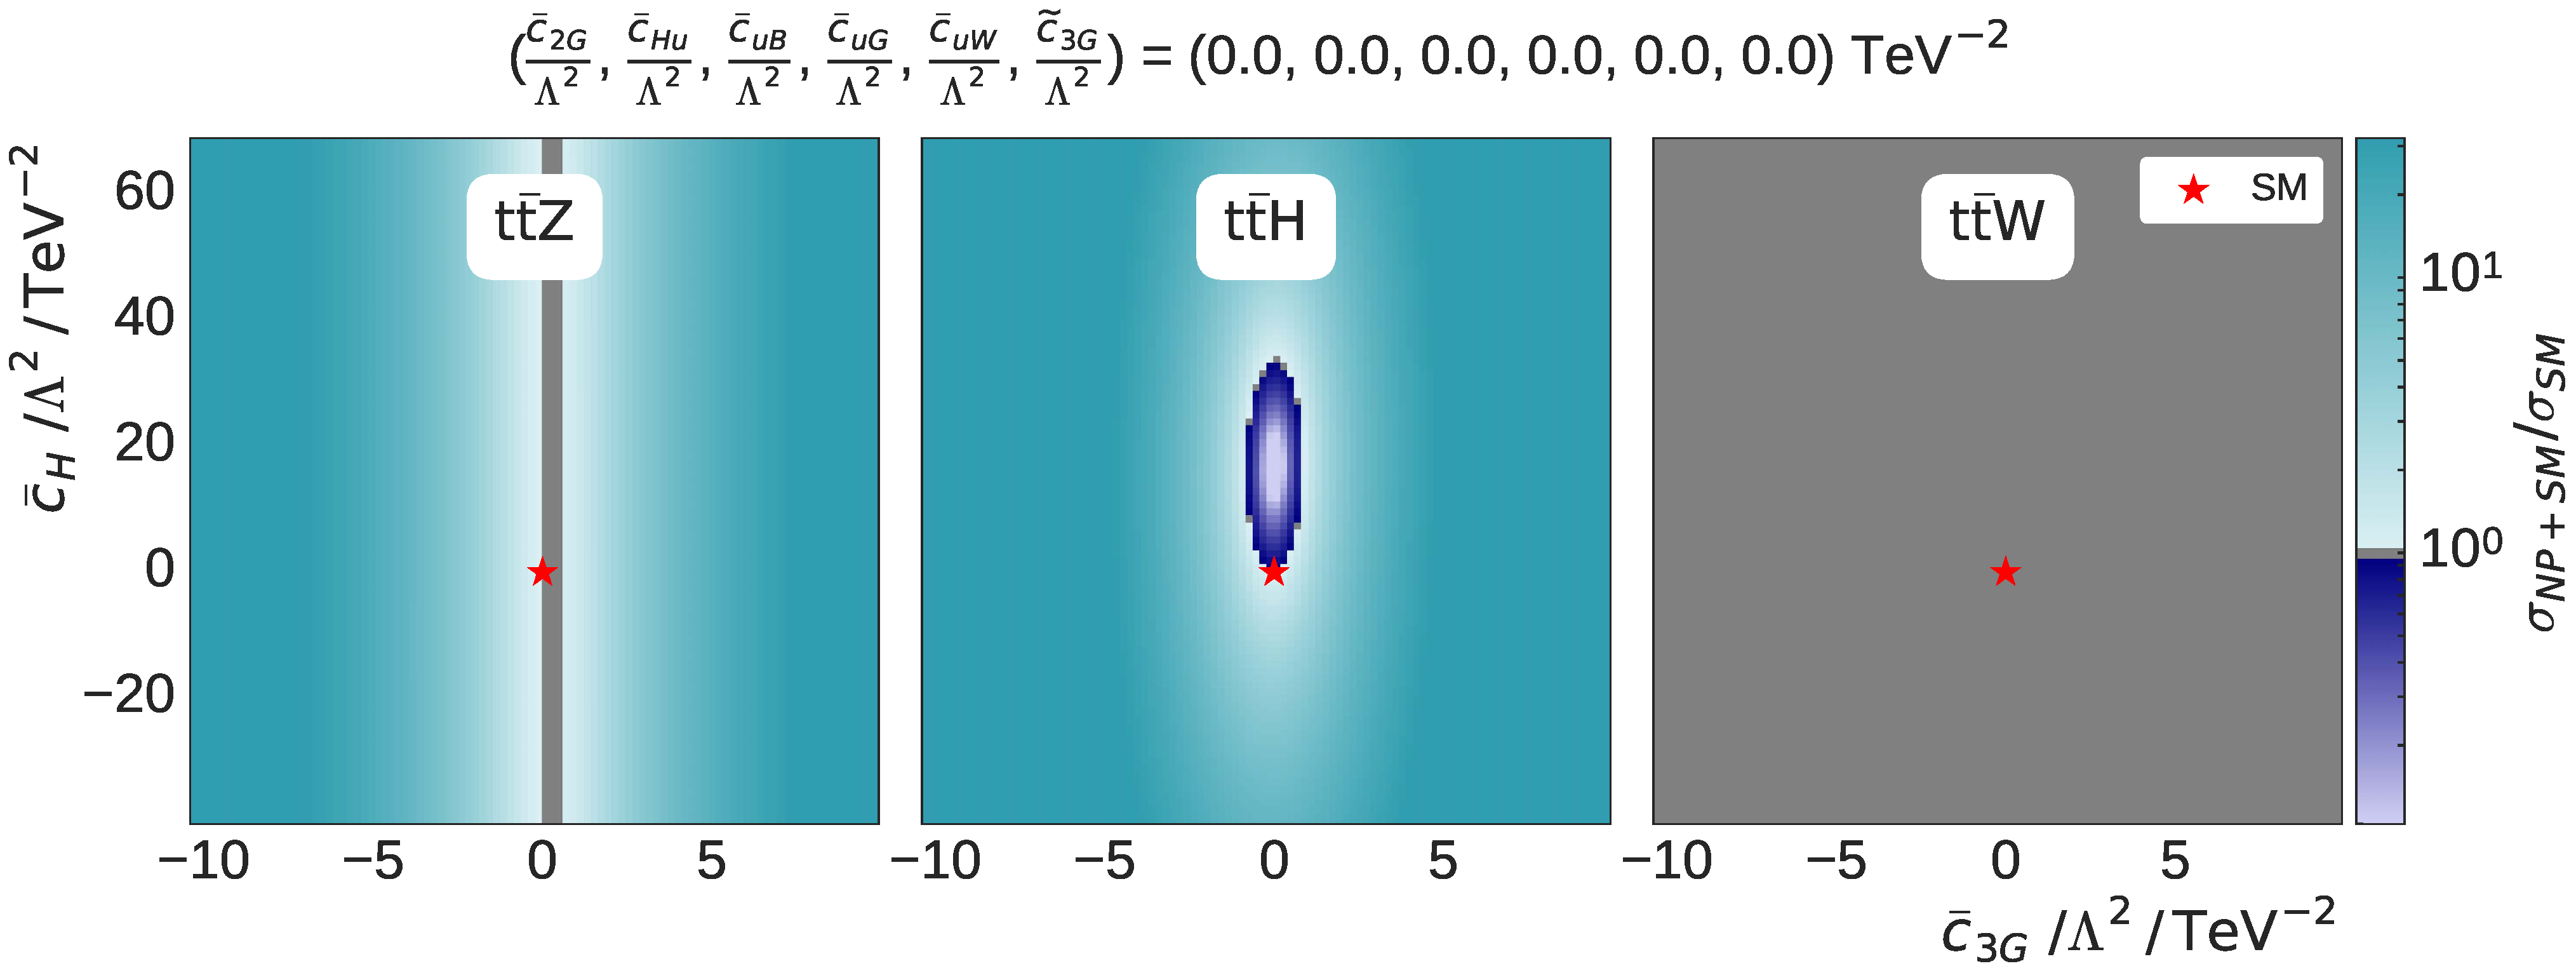
\includegraphics[width=\linewidth]{figures/thirteen-TeV/scaling-frozen/c3G_cH}
    \caption{}
  \end{subfigure}
  \begin{subfigure}{\linewidth}
    \centering
    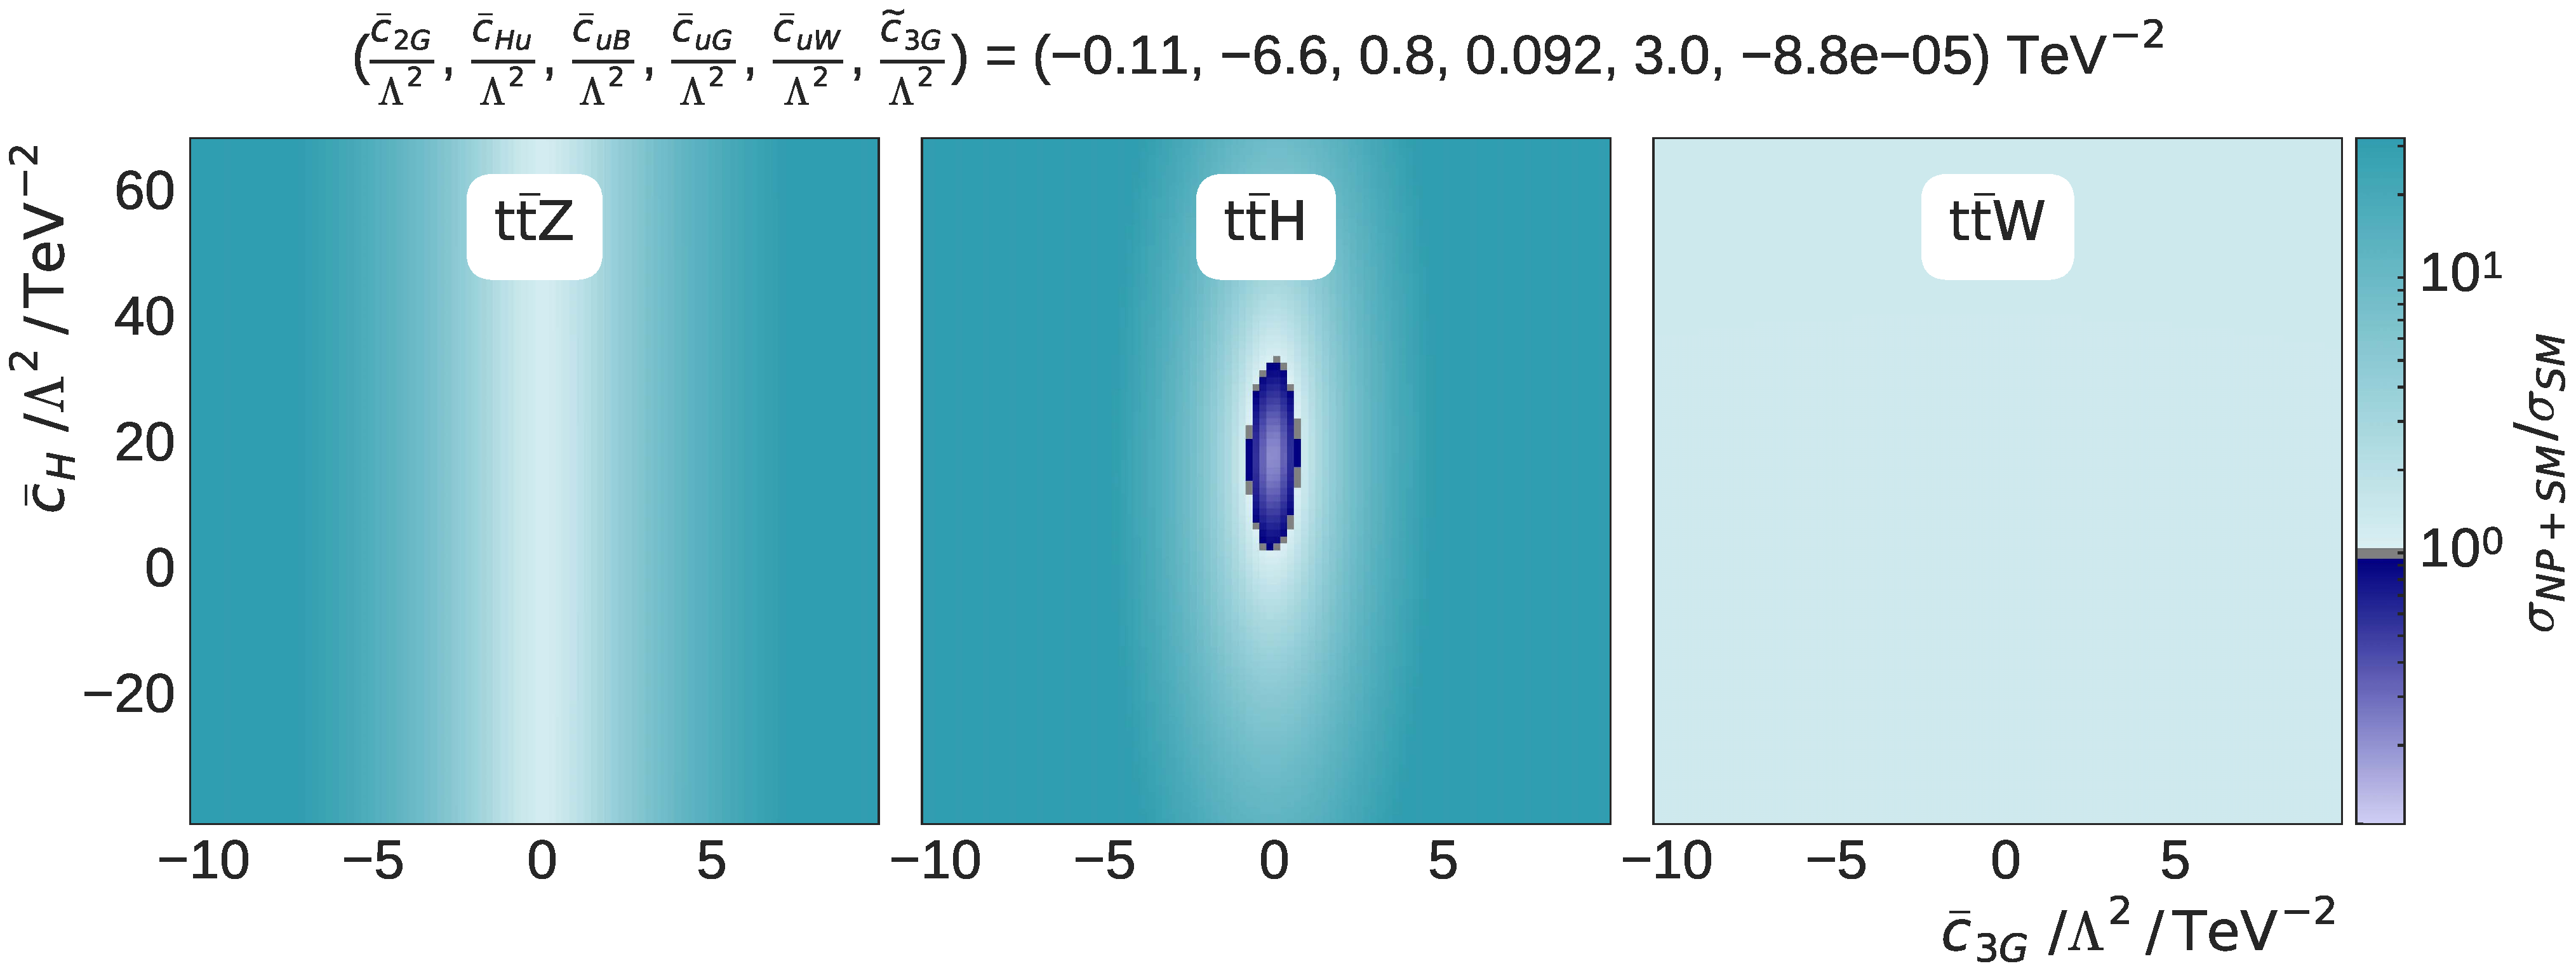
\includegraphics[width=\linewidth]{figures/thirteen-TeV/scaling/c3G_cH}
    \caption{}
  \end{subfigure}
  \begin{subfigure}{\linewidth}
    \centering
    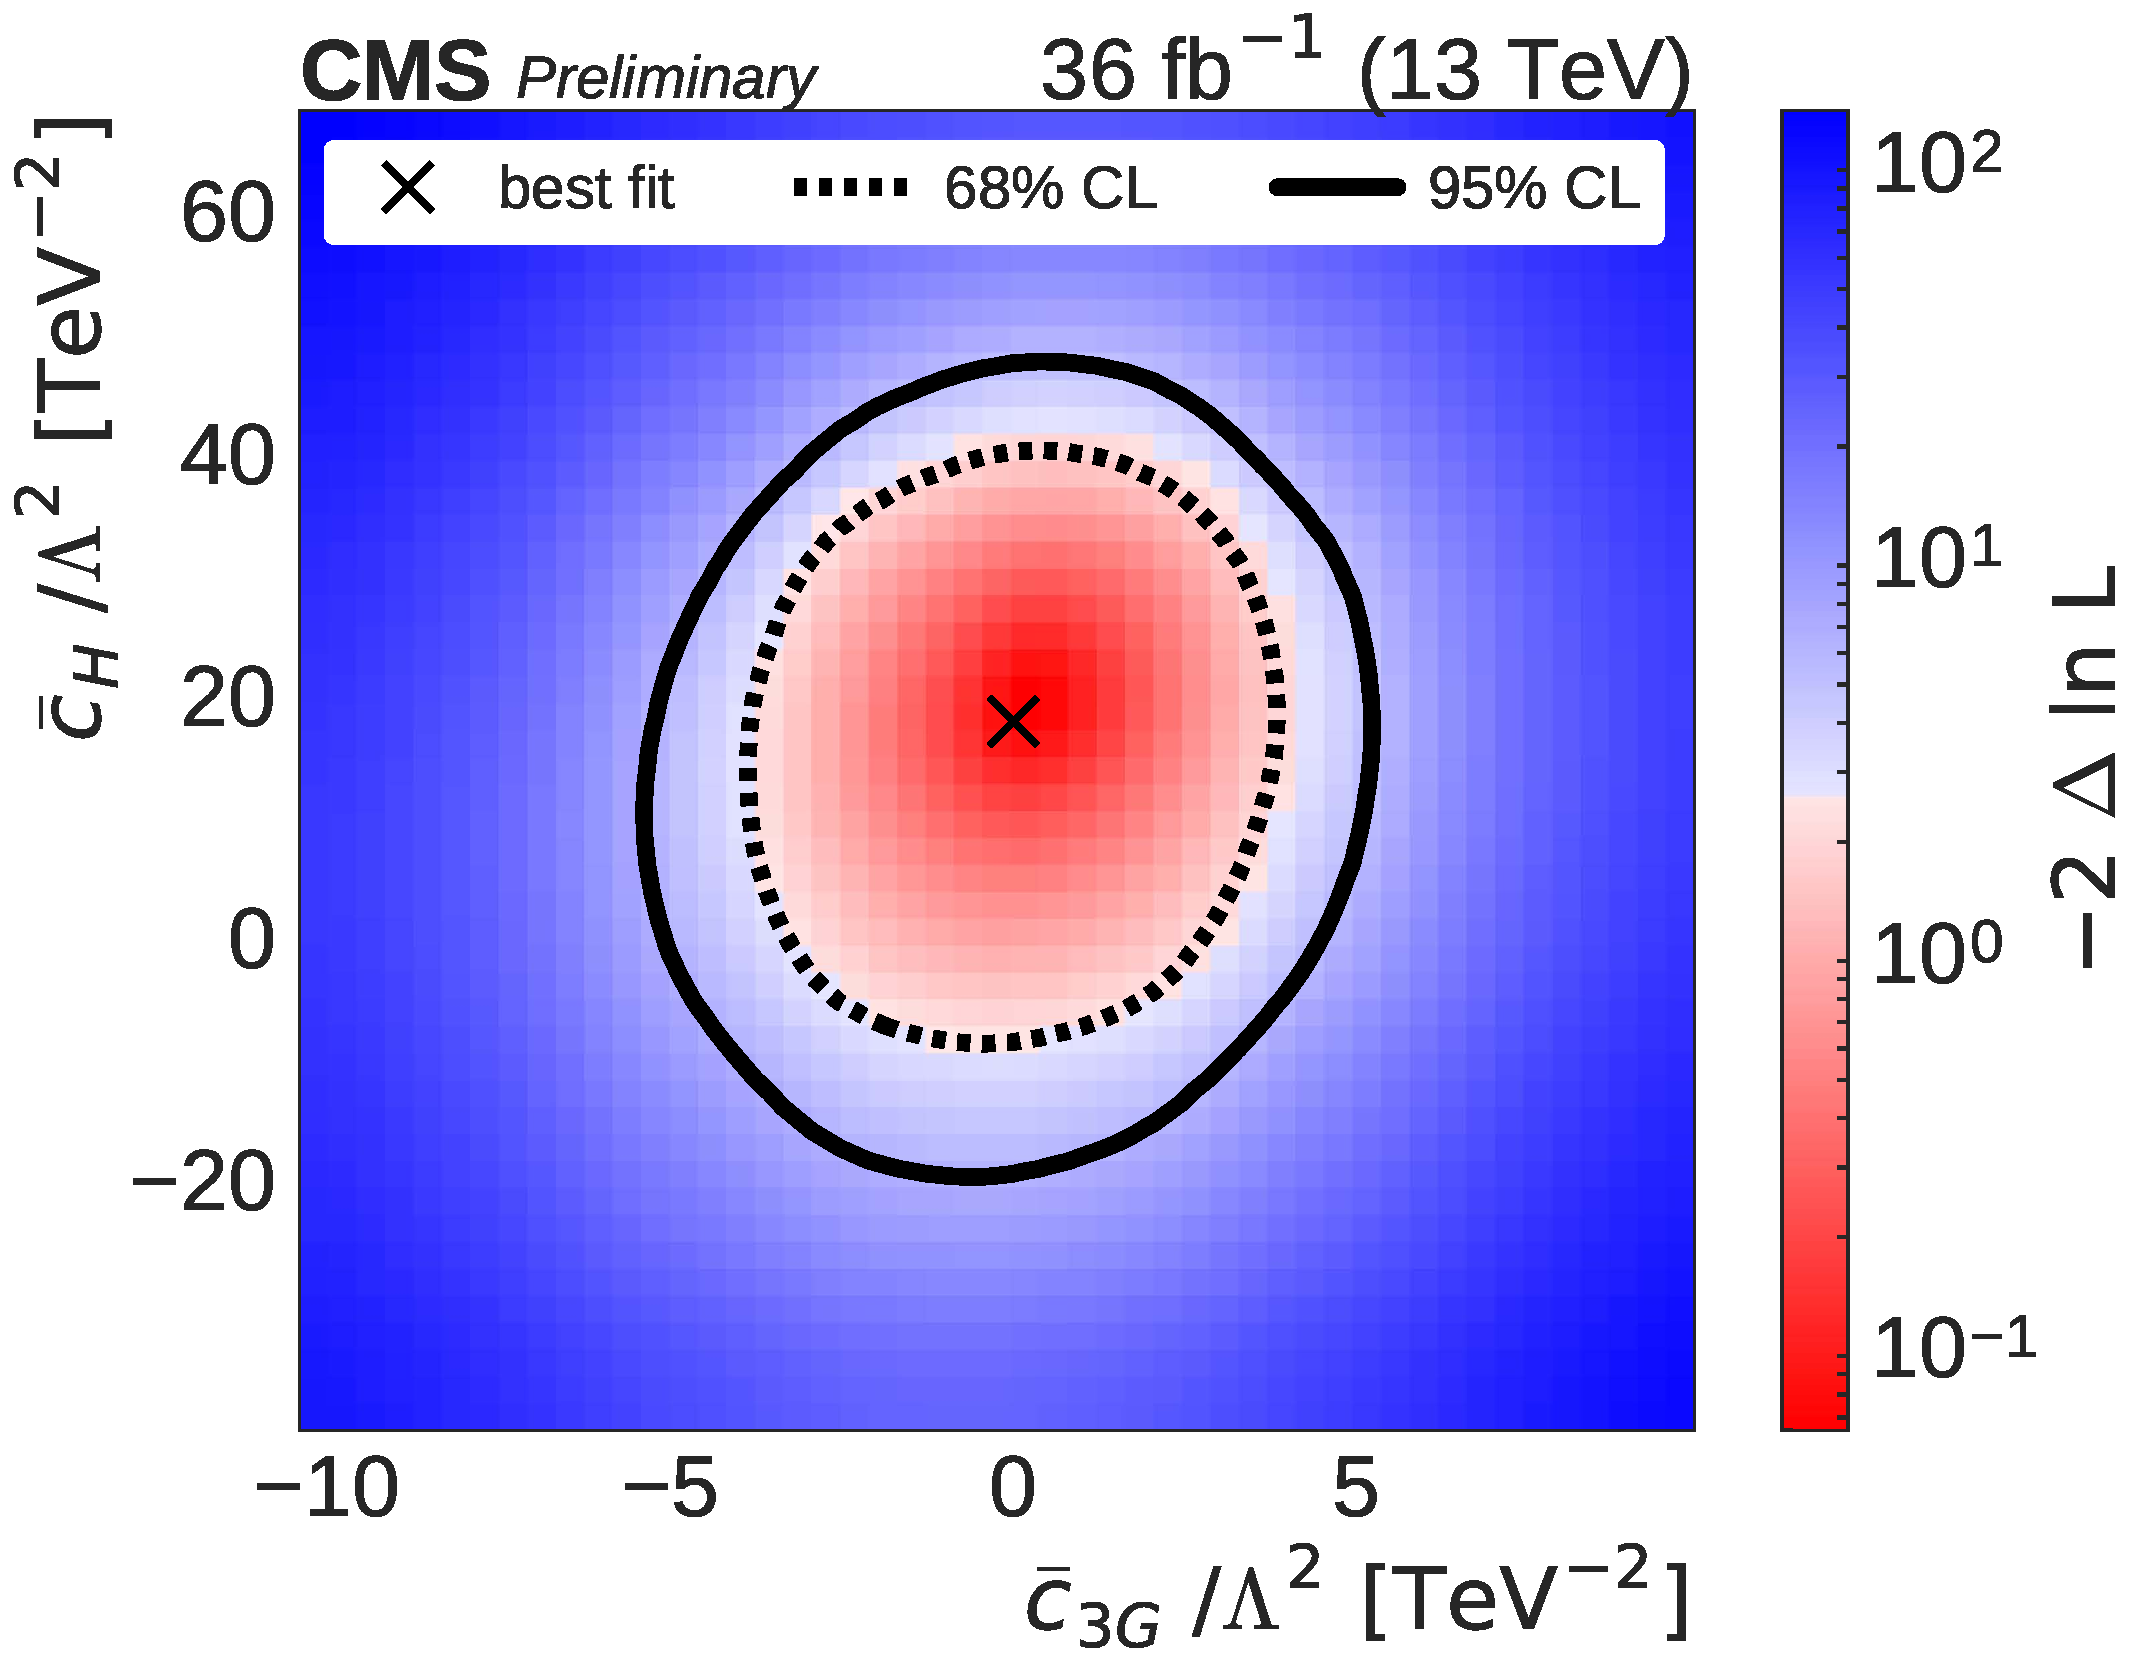
\includegraphics[width=0.6\linewidth]{figures/thirteen-TeV/nll/c3G_cH}
    \caption{}
  \end{subfigure}
  \vspace{-1cm}
  \setlength{\capwidth}{15cm}
  \caption[Signal scaling and profile likelihood scan in the \cH, \cthreeG plane]{Signal scaling
  shown in the \cH, \cthreeG plane with all other coefficients fixed to zero (a) or their best-fit
  values (b) for \ttZ (left), \ttH (center), and \ttW (right). The color represents the scaling
  ($\sigma_\text{NP + SM} / \sigma_\text{SM}$) due to NP effects. The star represents the SM point in
  which all $c_i=0$. The negative log likelihood is shown in (c). The best fit is represented by a
  cross. The \SI{68}{\percent} and \SI{95}{\percent} CL contours are shown with dashed and solid
  lines, respectively.}
\end{figure}

\begin{figure}
  \vspace{-1cm}
  \begin{subfigure}{\linewidth}
    \centering
    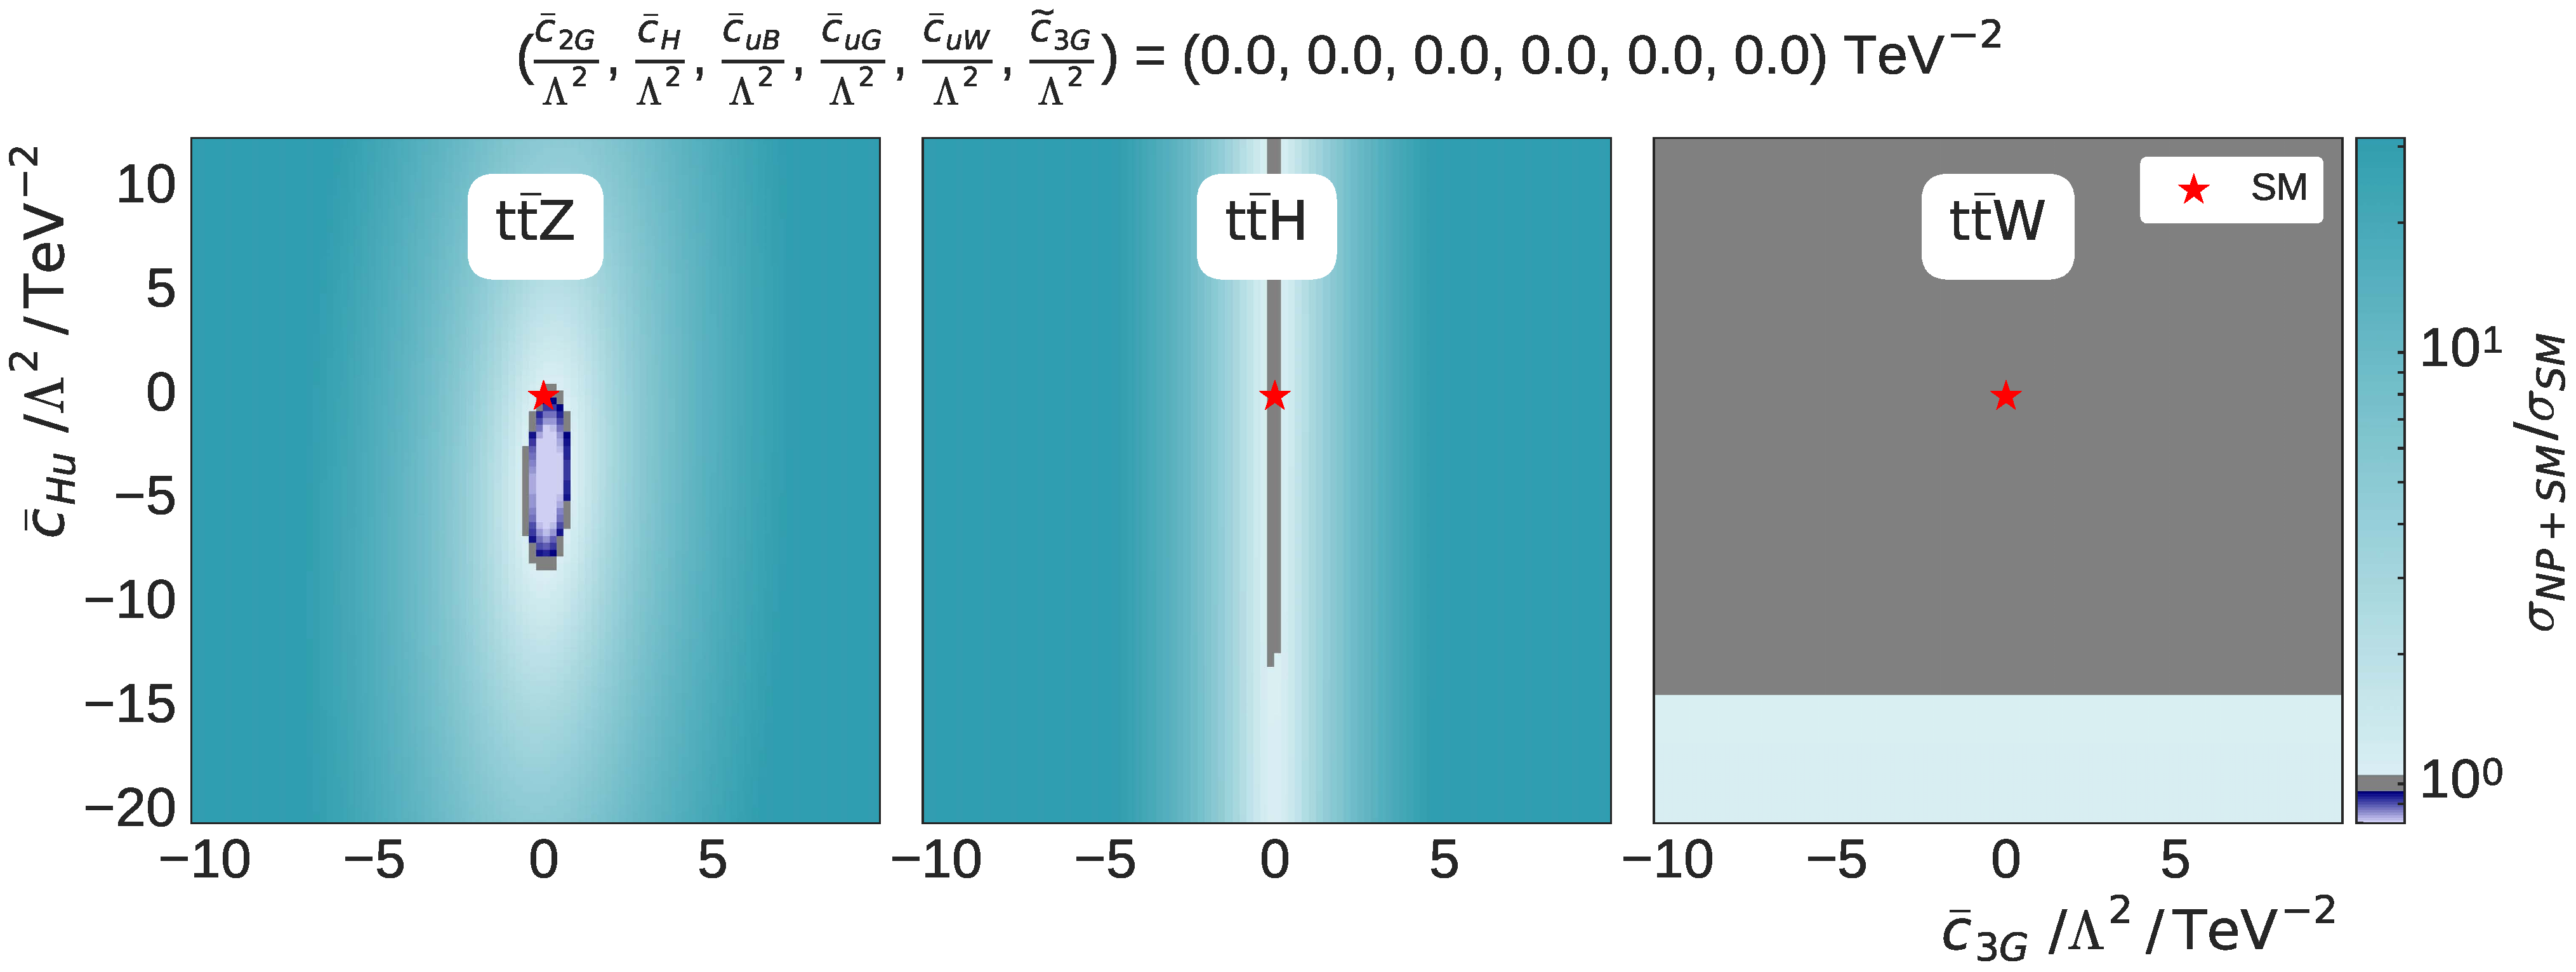
\includegraphics[width=\linewidth]{figures/thirteen-TeV/scaling-frozen/c3G_cHu}
    \caption{}
  \end{subfigure}
  \begin{subfigure}{\linewidth}
    \centering
    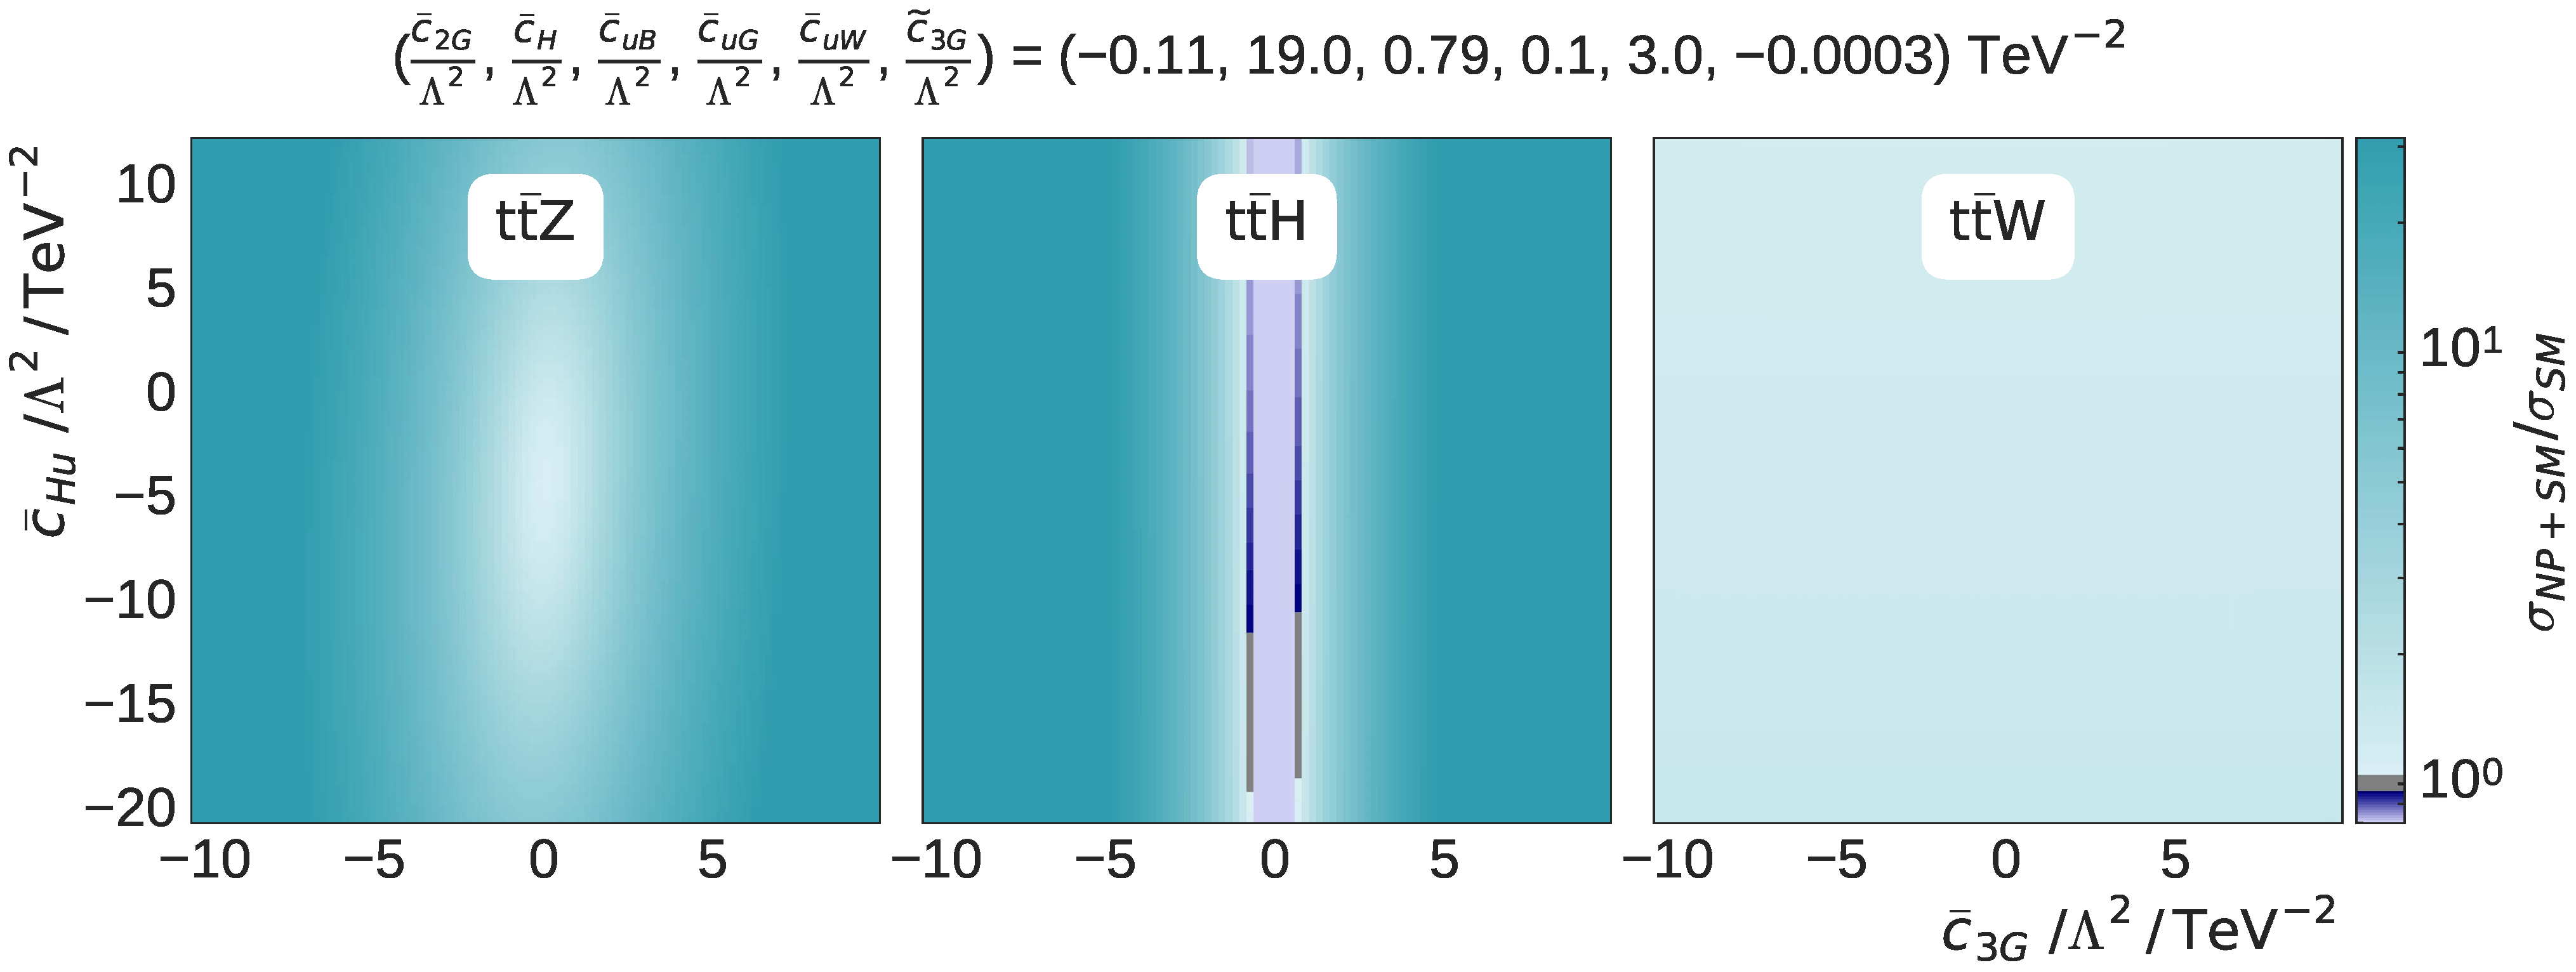
\includegraphics[width=\linewidth]{figures/thirteen-TeV/scaling/c3G_cHu}
    \caption{}
  \end{subfigure}
  \begin{subfigure}{\linewidth}
    \centering
    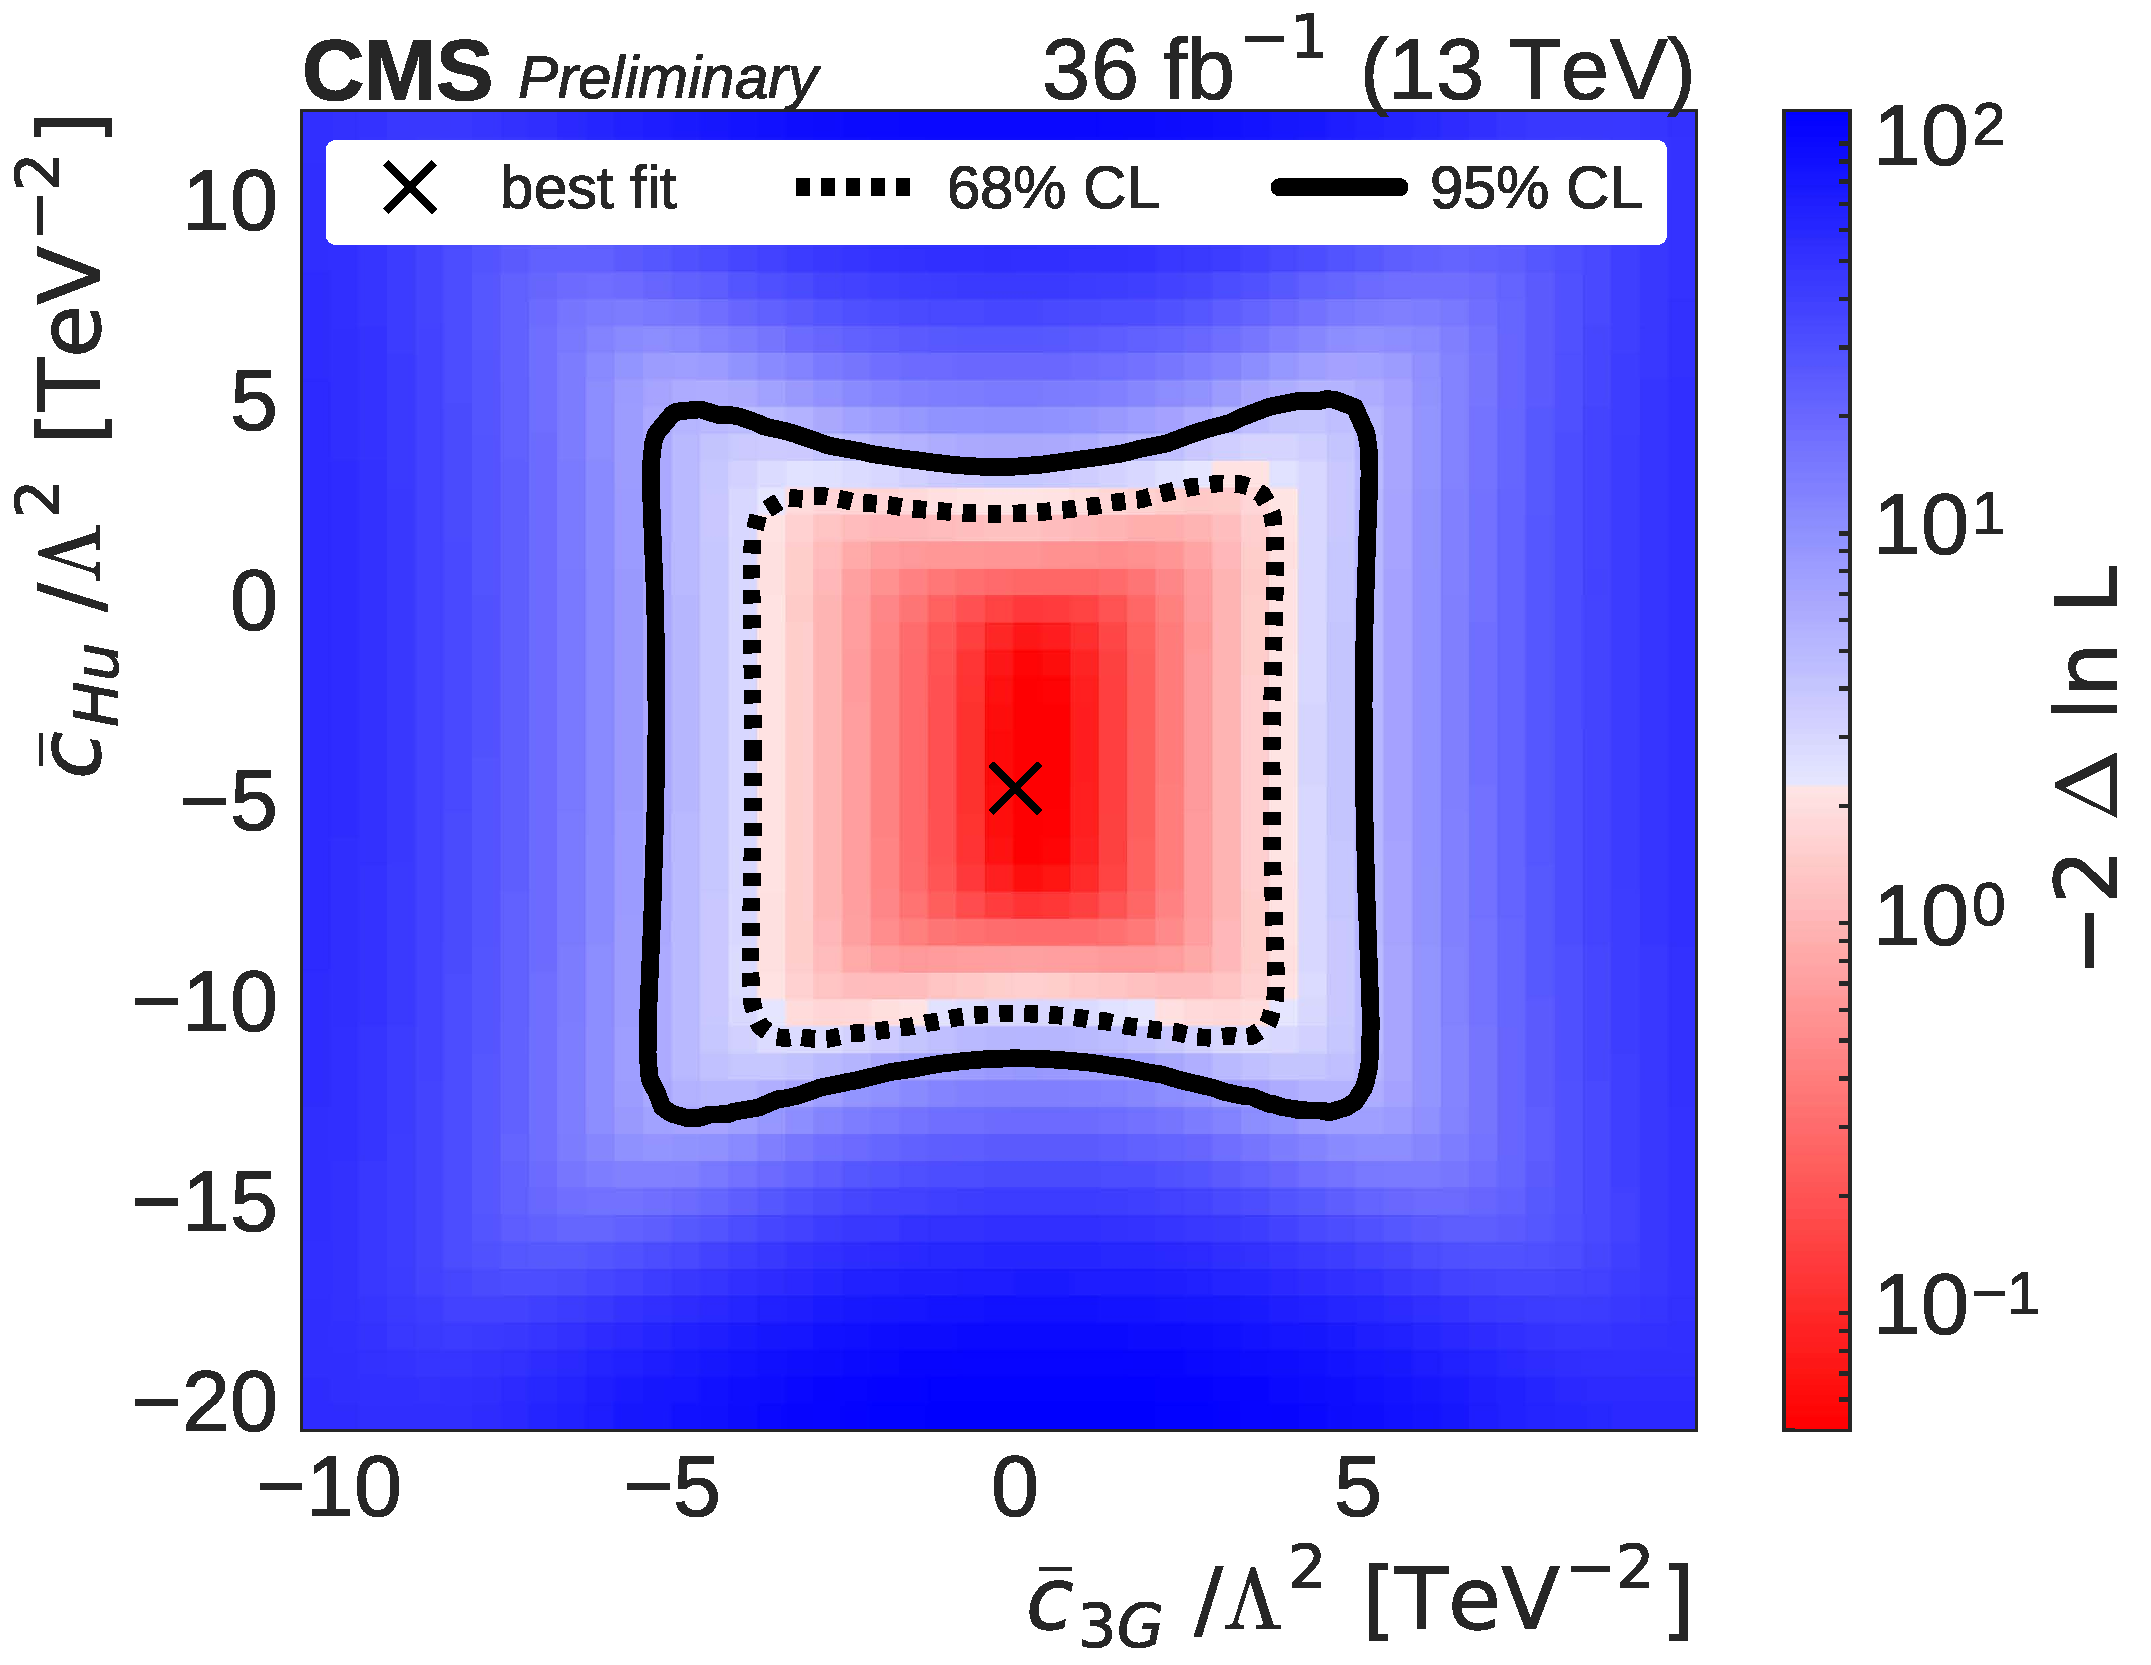
\includegraphics[width=0.6\linewidth]{figures/thirteen-TeV/nll/c3G_cHu}
    \caption{}
  \end{subfigure}
  \vspace{-1cm}
  \setlength{\capwidth}{15cm}
  \caption[Signal scaling and profile likelihood scan in the \cHu, \cthreeG plane]{Signal scaling
  shown in the \cHu, \cthreeG plane with all other coefficients fixed to zero (a) or their best-fit
  values (b) for \ttZ (left), \ttH (center), and \ttW (right). The color represents the scaling
  ($\sigma_\text{NP + SM} / \sigma_\text{SM}$) due to NP effects. The star represents the SM point in
  which all $c_i=0$. The negative log likelihood is shown in (c). The best fit is represented by a
  cross. The \SI{68}{\percent} and \SI{95}{\percent} CL contours are shown with dashed and solid
  lines, respectively.}
\end{figure}

\begin{figure}
  \vspace{-1cm}
  \begin{subfigure}{\linewidth}
    \centering
    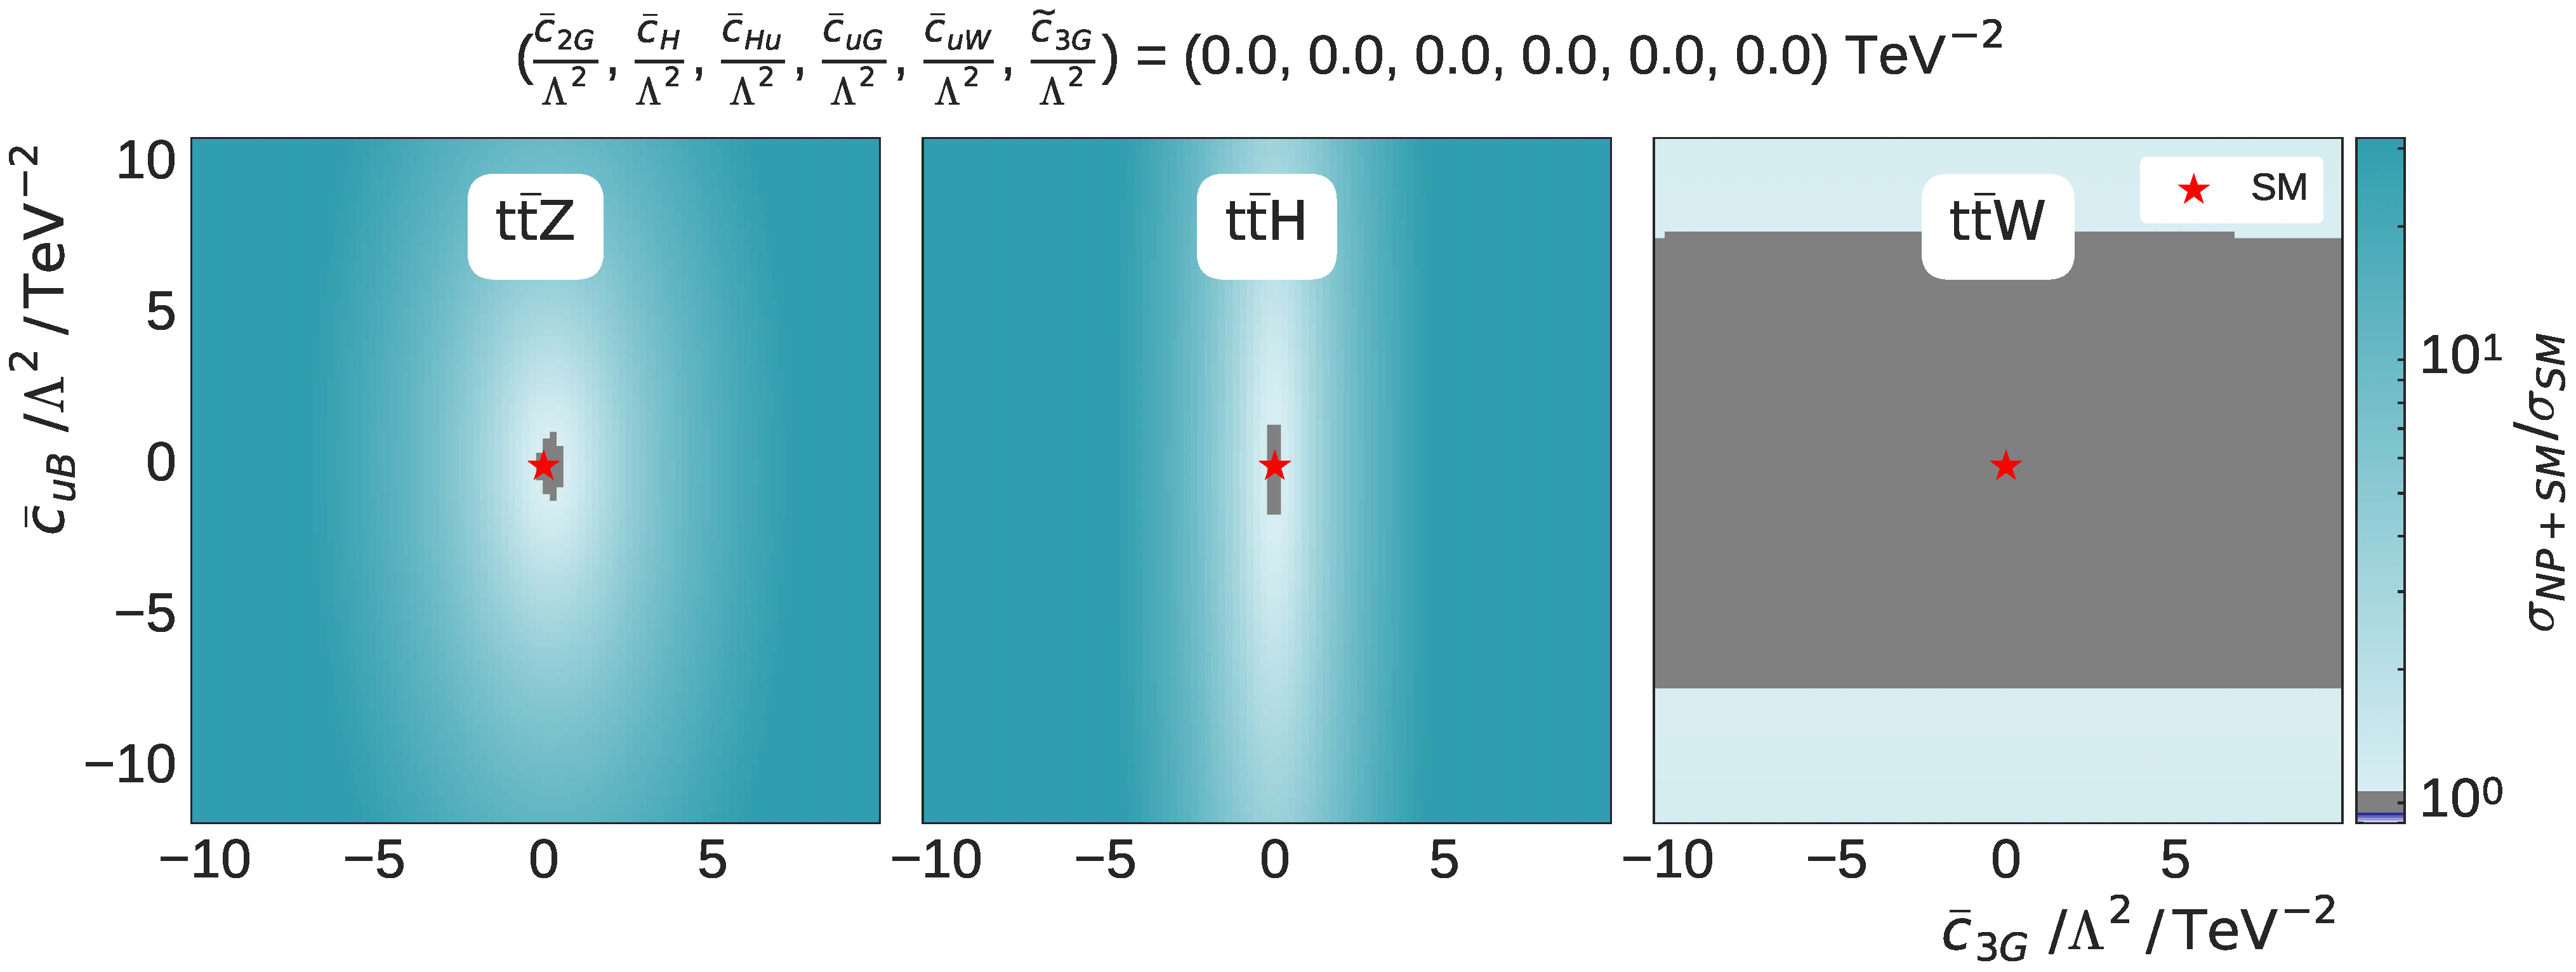
\includegraphics[width=\linewidth]{figures/thirteen-TeV/scaling-frozen/c3G_cuB}
    \caption{}
  \end{subfigure}
  \begin{subfigure}{\linewidth}
    \centering
    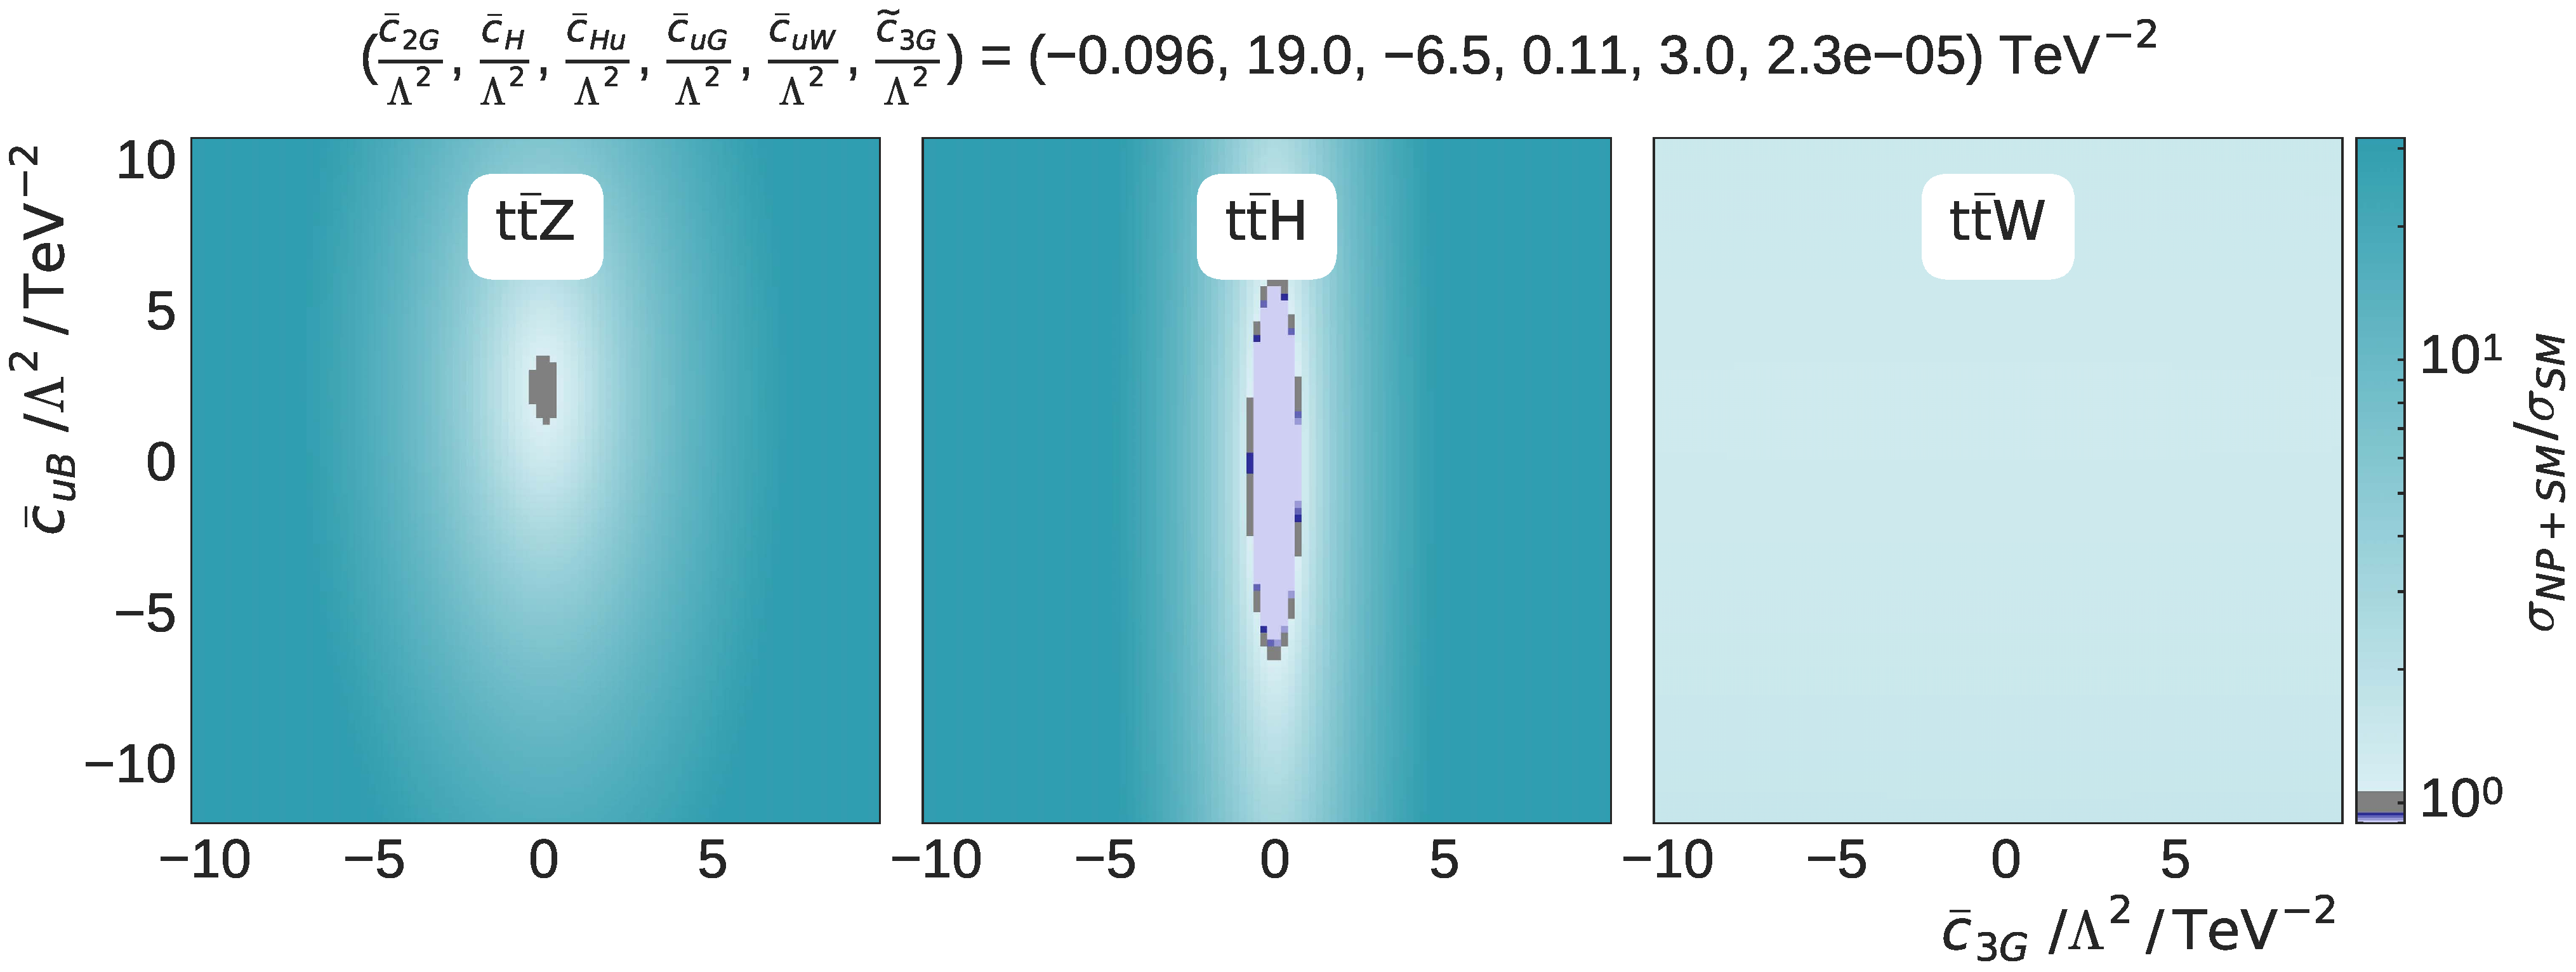
\includegraphics[width=\linewidth]{figures/thirteen-TeV/scaling/c3G_cuB}
    \caption{}
  \end{subfigure}
  \begin{subfigure}{\linewidth}
    \centering
    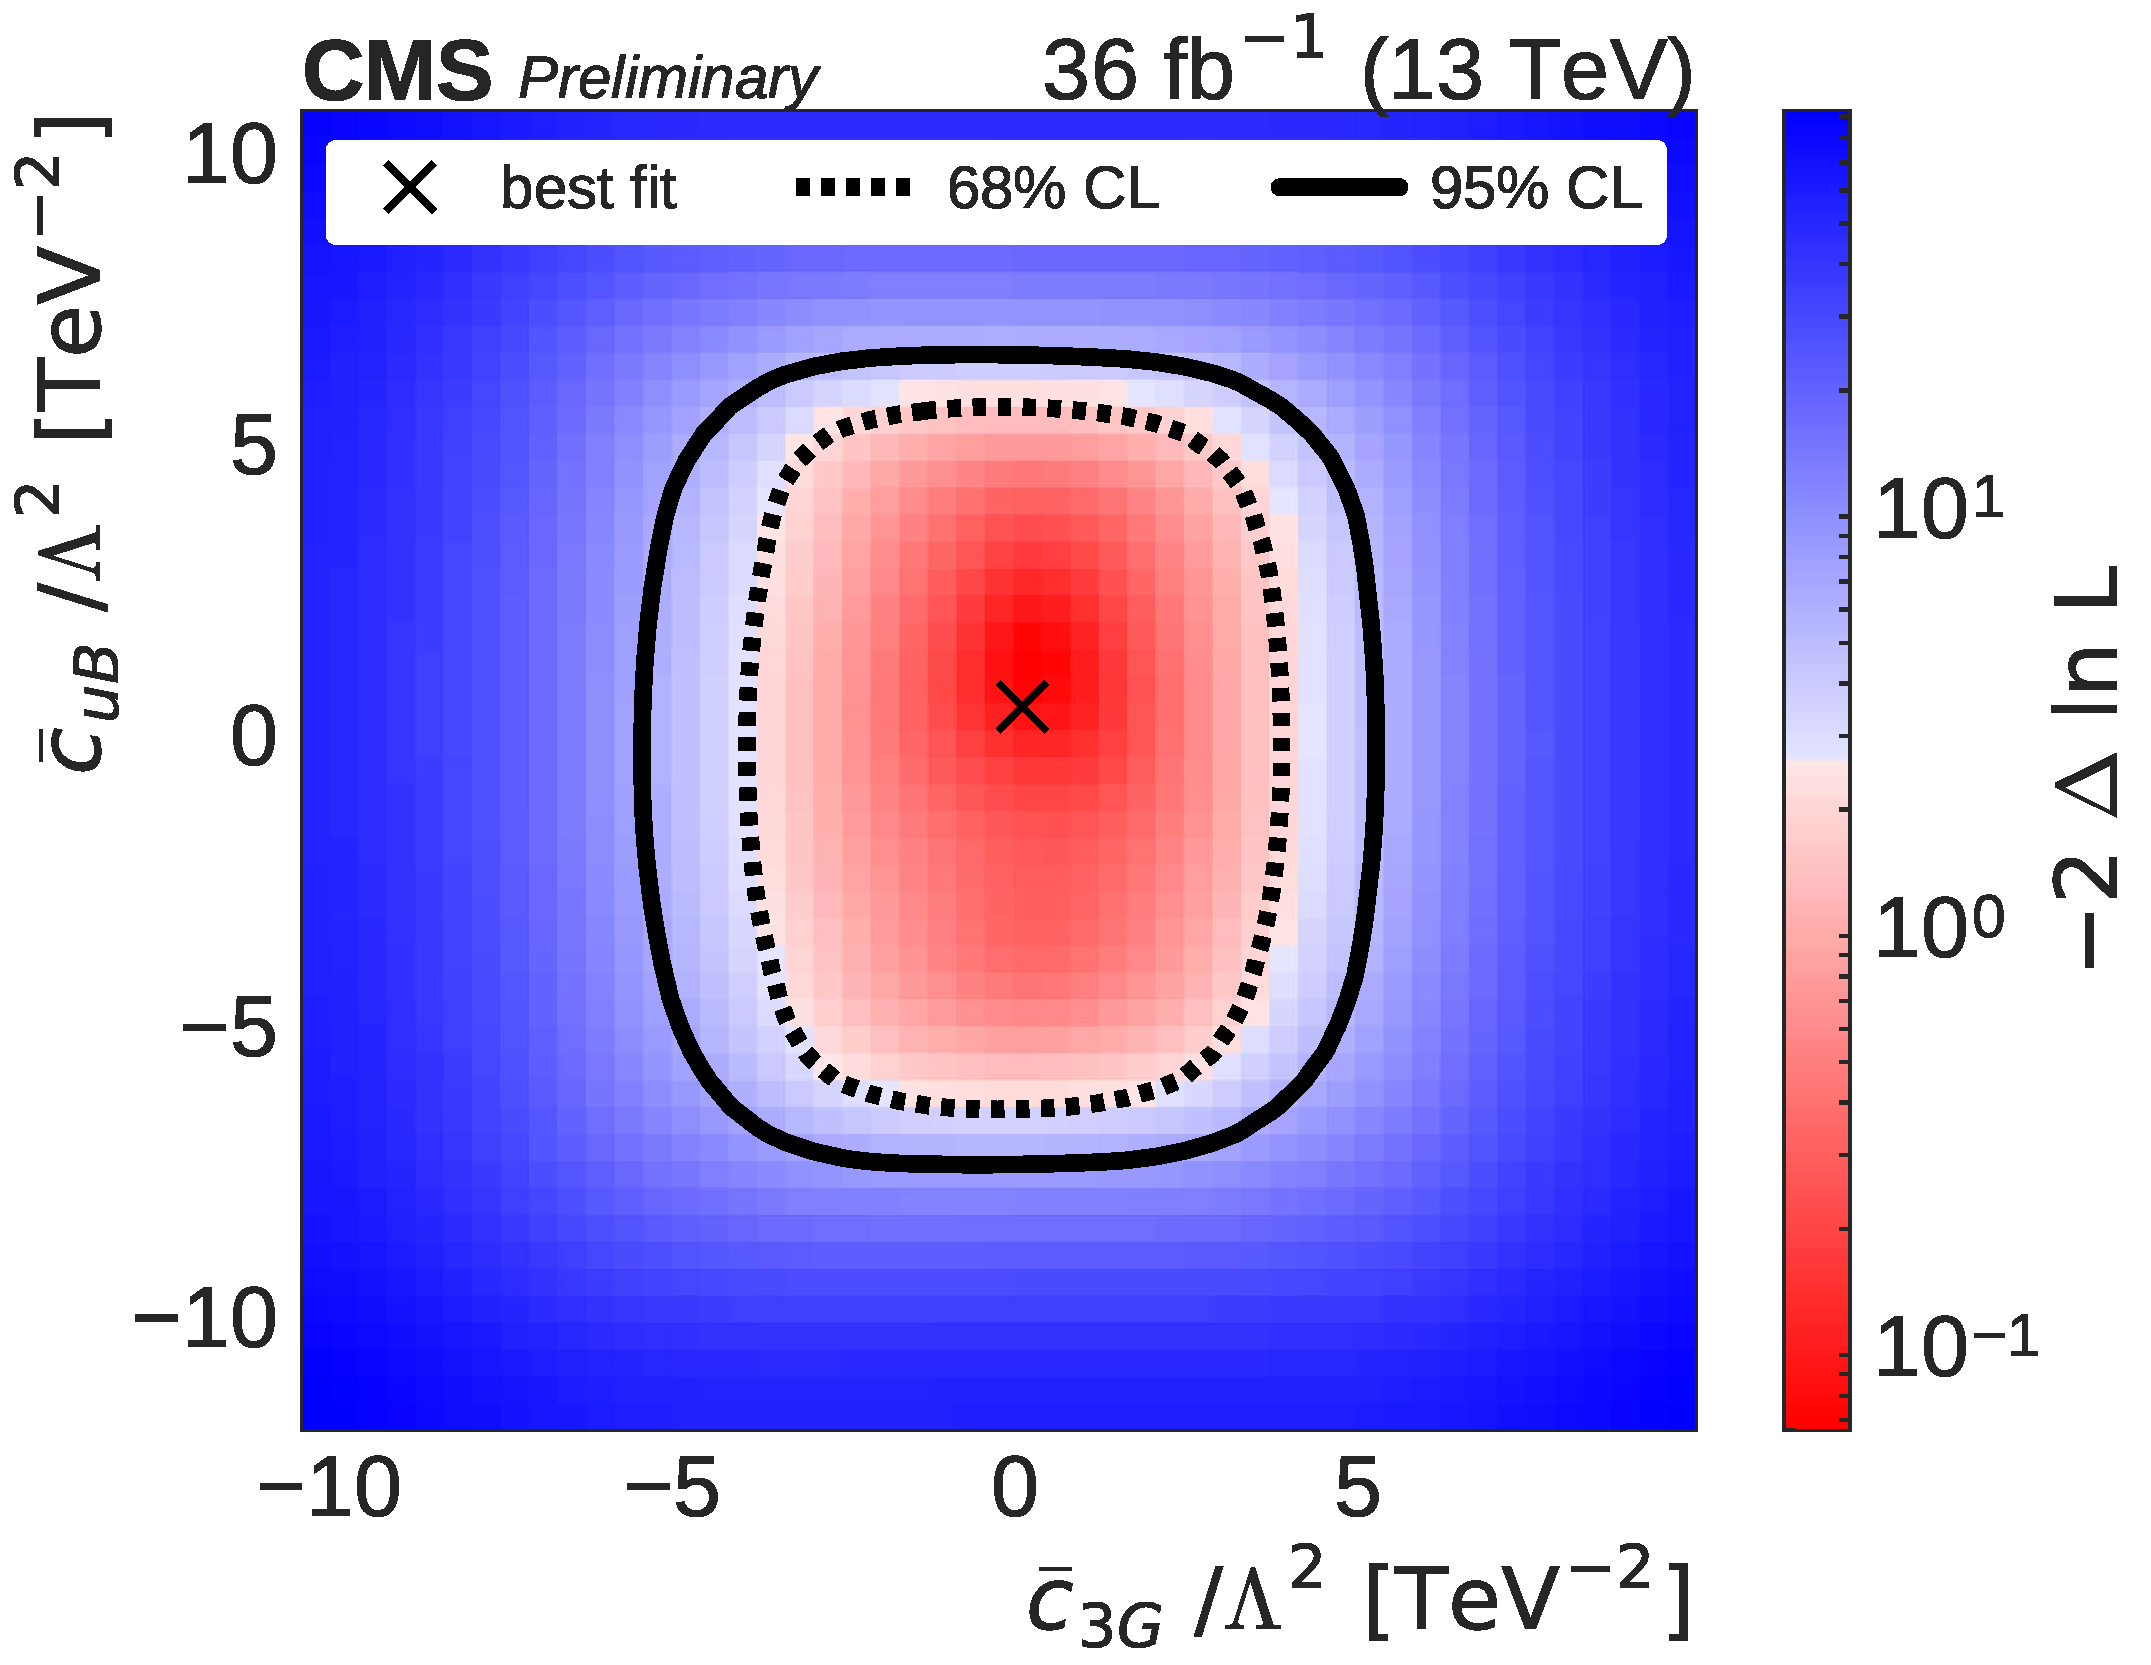
\includegraphics[width=0.6\linewidth]{figures/thirteen-TeV/nll/c3G_cuB}
    \caption{}
  \end{subfigure}
  \vspace{-1cm}
  \setlength{\capwidth}{15cm}
  \caption[Signal scaling and profile likelihood scan in the \cthreeG, \cuB plane]{Signal scaling
  shown in the \cthreeG, \cuB plane with all other coefficients fixed to zero (a) or their best-fit
  values (b) for \ttZ (left), \ttH (center), and \ttW (right). The color represents the scaling
  ($\sigma_\text{NP + SM} / \sigma_\text{SM}$) due to NP effects. The star represents the SM point in
  which all $c_i=0$. The negative log likelihood is shown in (c). The best fit is represented by a
  cross. The \SI{68}{\percent} and \SI{95}{\percent} CL contours are shown with dashed and solid
  lines, respectively.}
\end{figure}

\begin{figure}
  \vspace{-1cm}
  \begin{subfigure}{\linewidth}
    \centering
    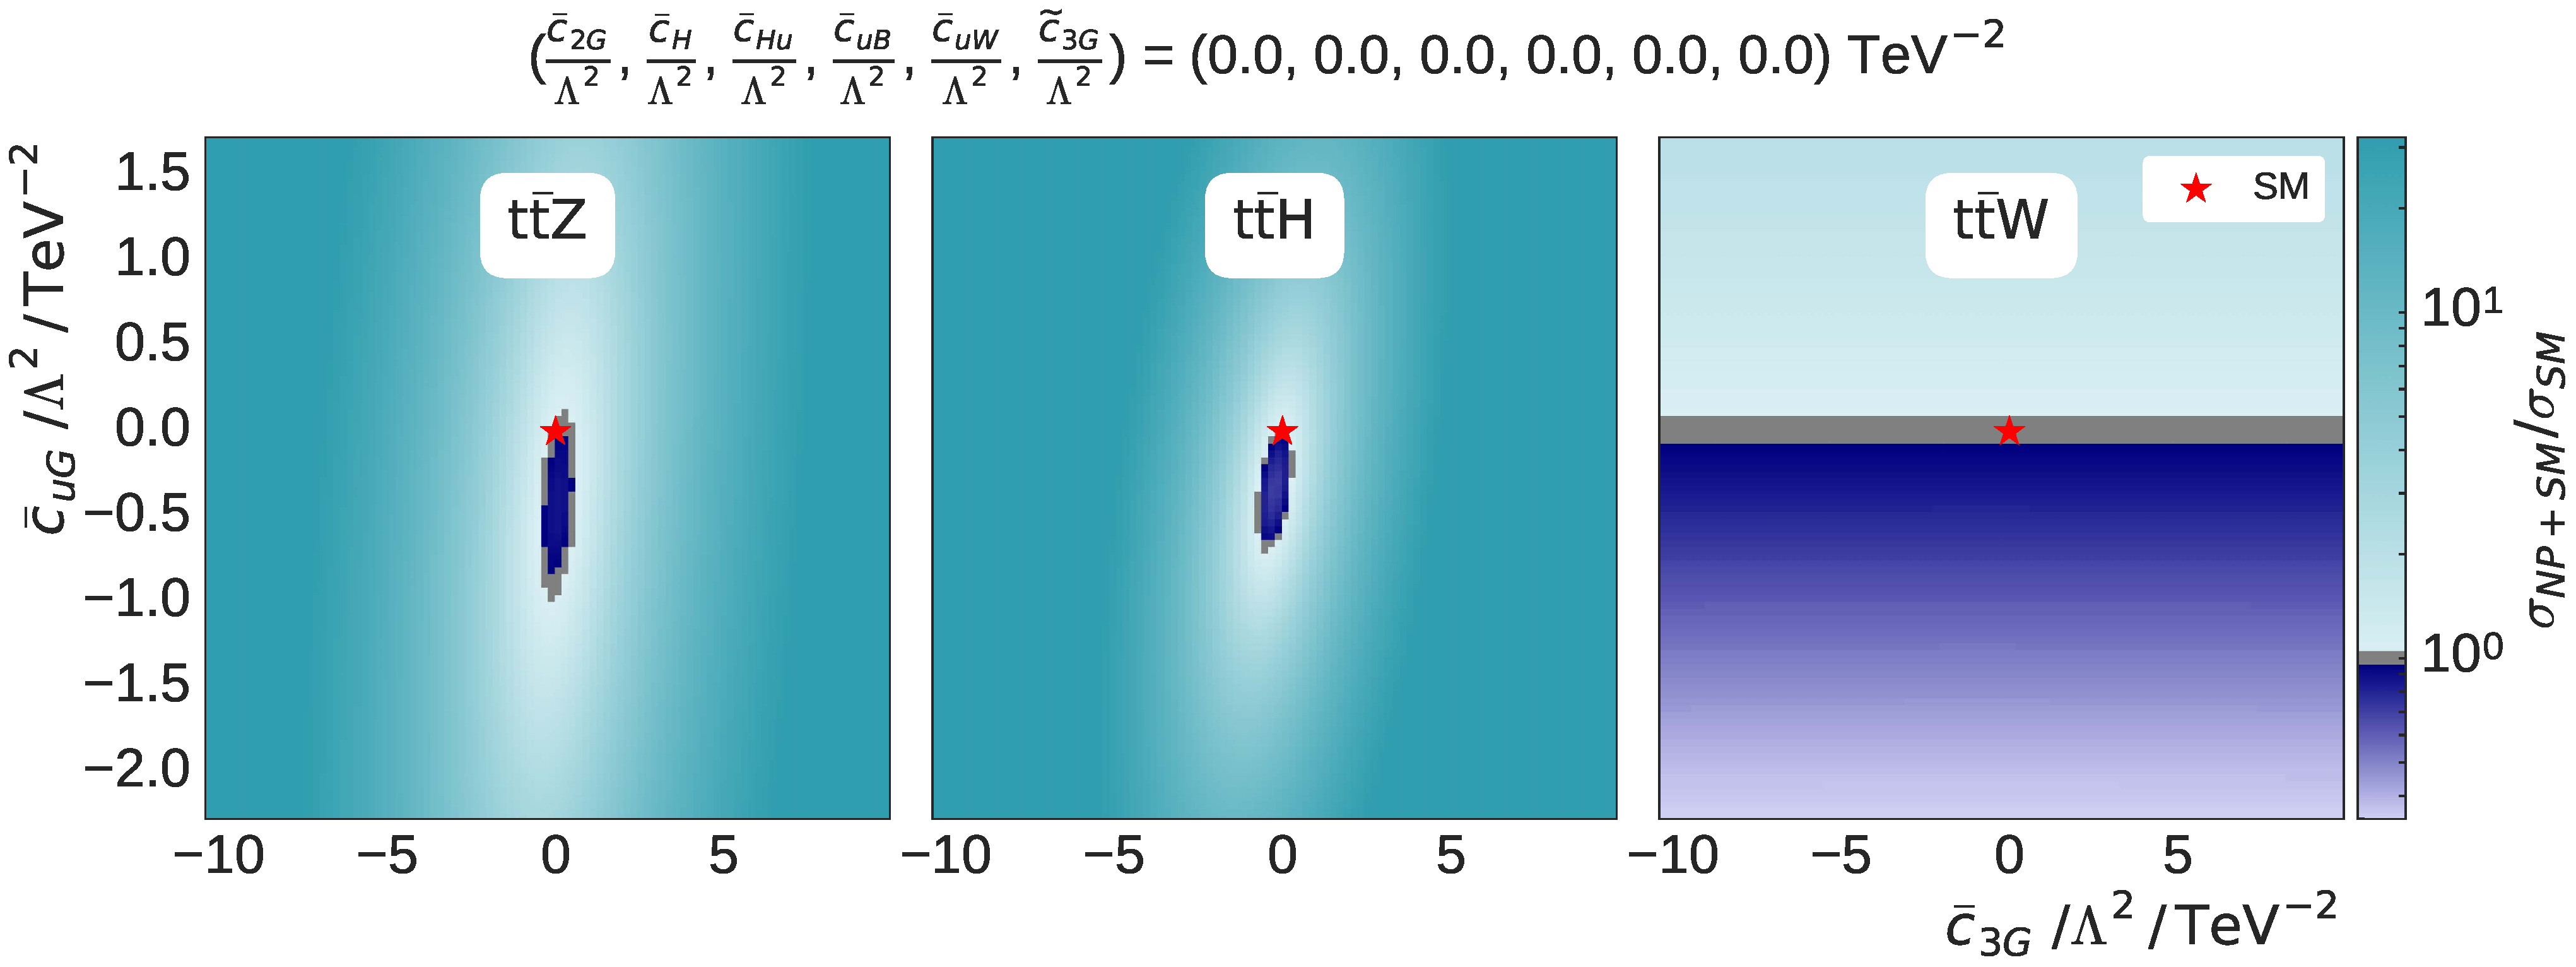
\includegraphics[width=\linewidth]{figures/thirteen-TeV/scaling-frozen/c3G_cuG}
    \caption{}
  \end{subfigure}
  \begin{subfigure}{\linewidth}
    \centering
    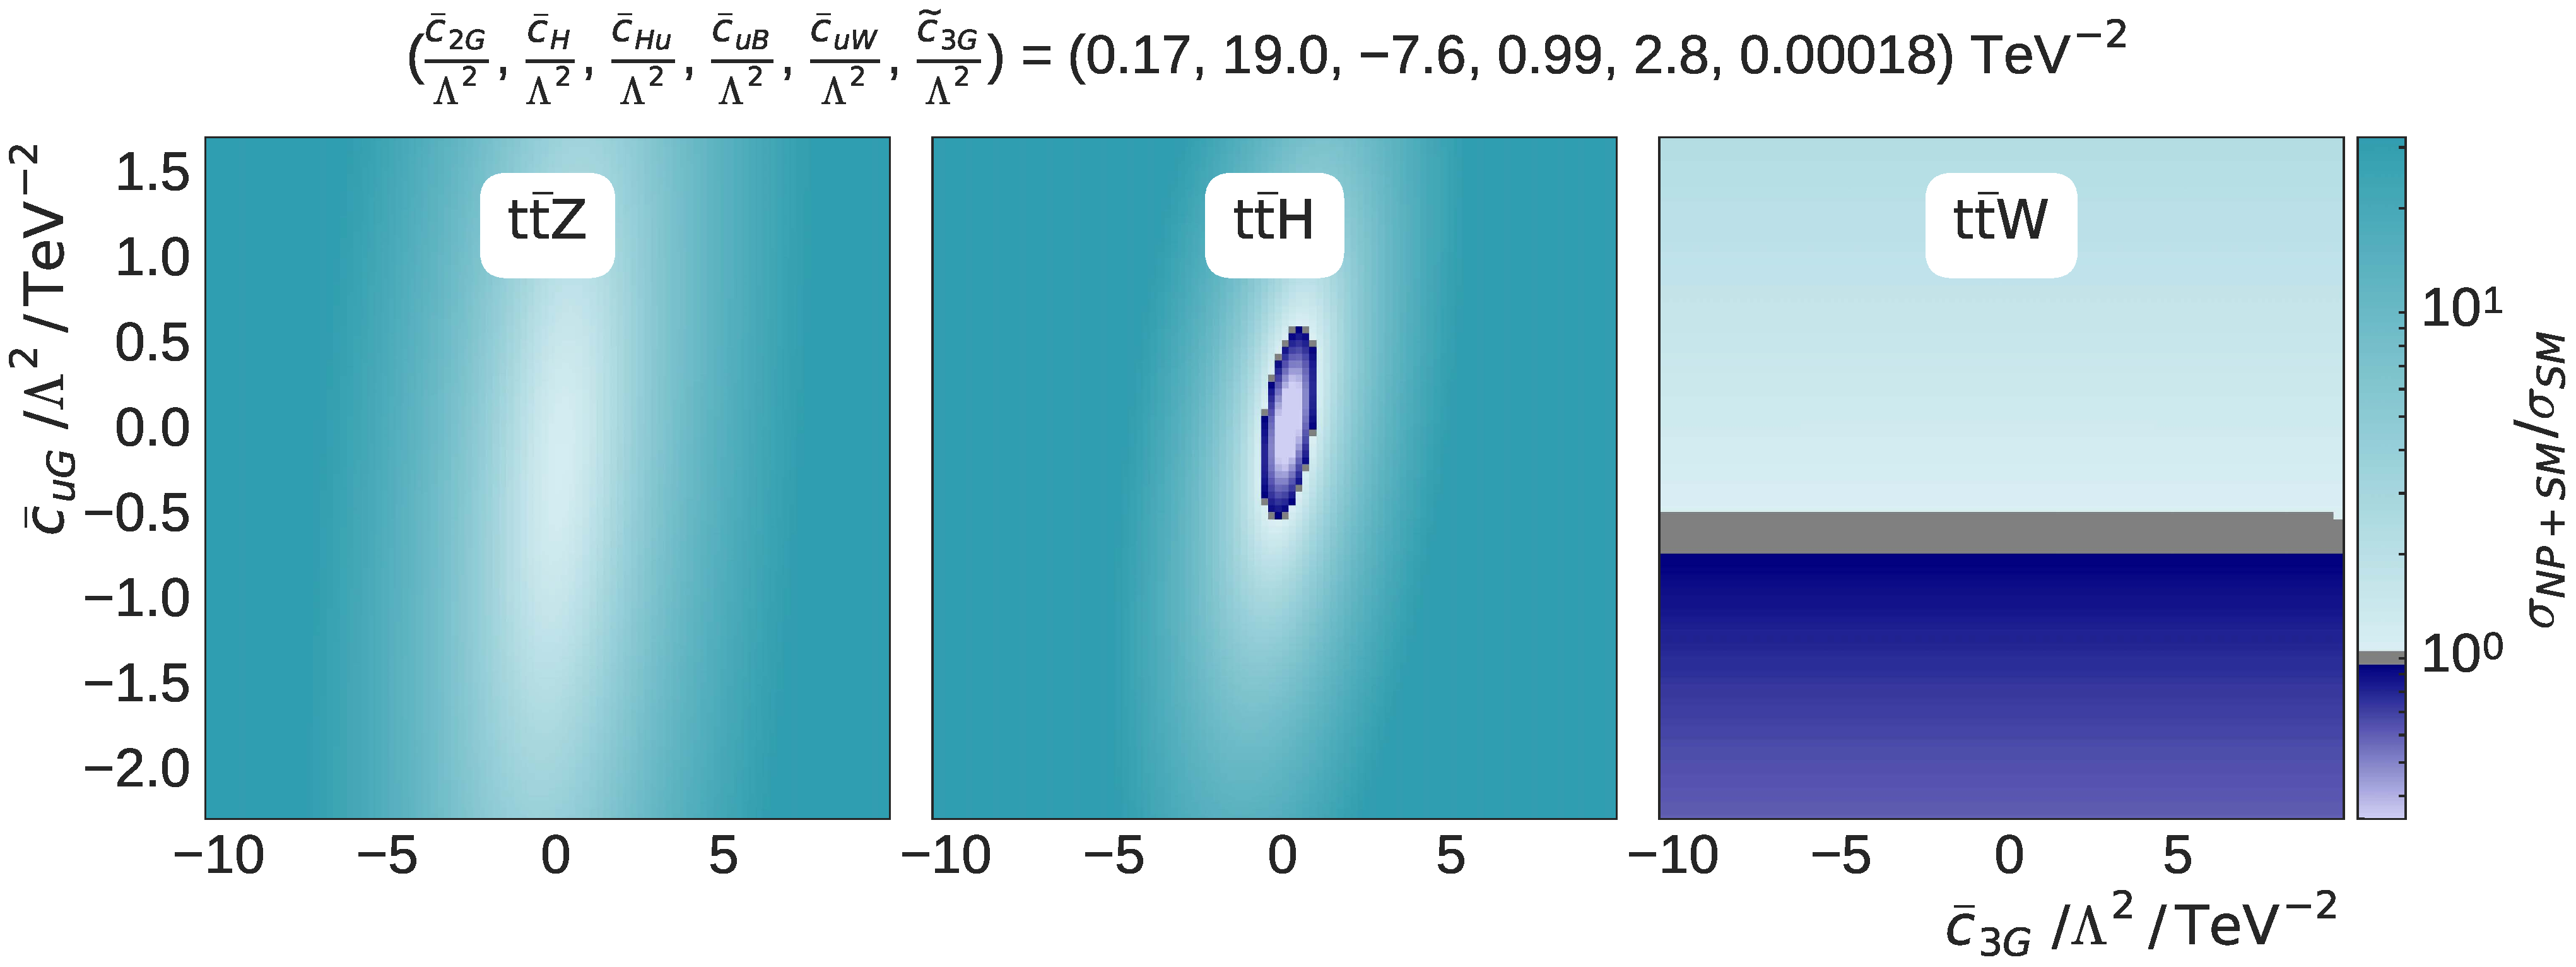
\includegraphics[width=\linewidth]{figures/thirteen-TeV/scaling/c3G_cuG}
    \caption{}
  \end{subfigure}
  \begin{subfigure}{\linewidth}
    \centering
    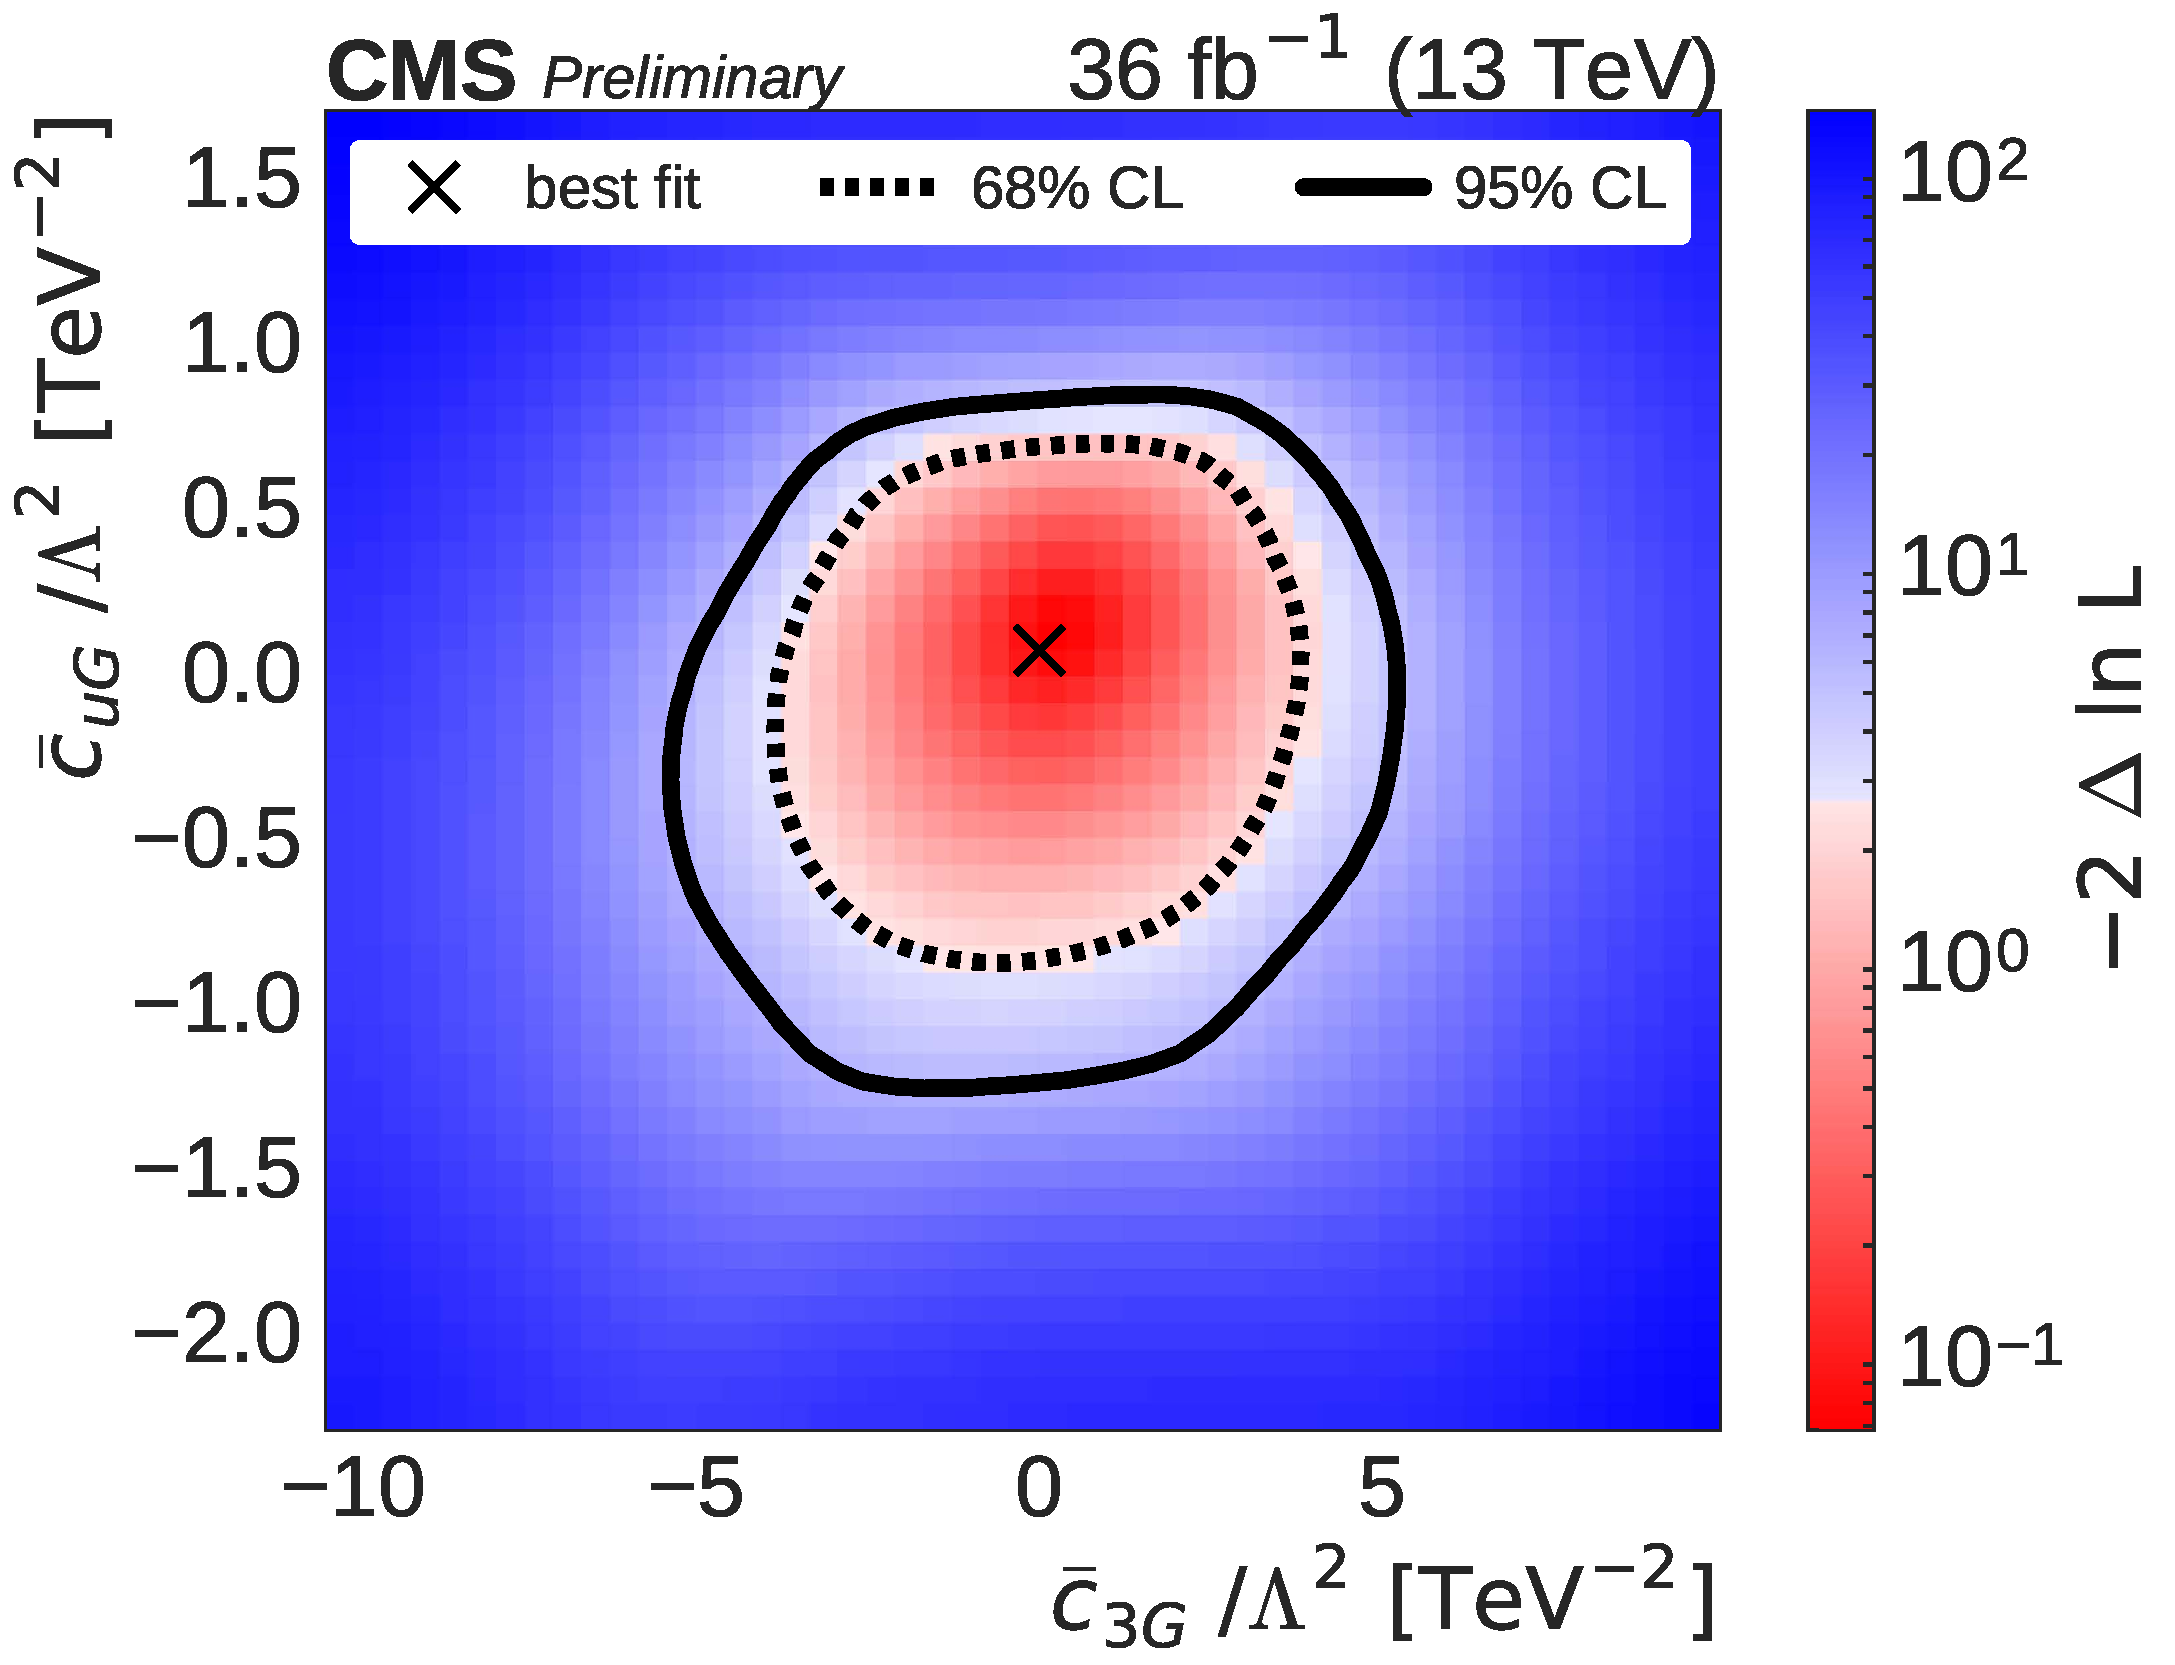
\includegraphics[width=0.6\linewidth]{figures/thirteen-TeV/nll/c3G_cuG}
    \caption{}
  \end{subfigure}
  \vspace{-1cm}
  \setlength{\capwidth}{15cm}
  \caption[Signal scaling and profile likelihood scan in the \cthreeG, \cuG plane]{Signal scaling
  shown in the \cthreeG, \cuG plane with all other coefficients fixed to zero (a) or their best-fit
  values (b) for \ttZ (left), \ttH (center), and \ttW (right). The color represents the scaling
  ($\sigma_\text{NP + SM} / \sigma_\text{SM}$) due to NP effects. The star represents the SM point in
  which all $c_i=0$. The negative log likelihood is shown in (c). The best fit is represented by a
  cross. The \SI{68}{\percent} and \SI{95}{\percent} CL contours are shown with dashed and solid
  lines, respectively.}
\end{figure}

\begin{figure}
  \vspace{-1cm}
  \begin{subfigure}{\linewidth}
    \centering
    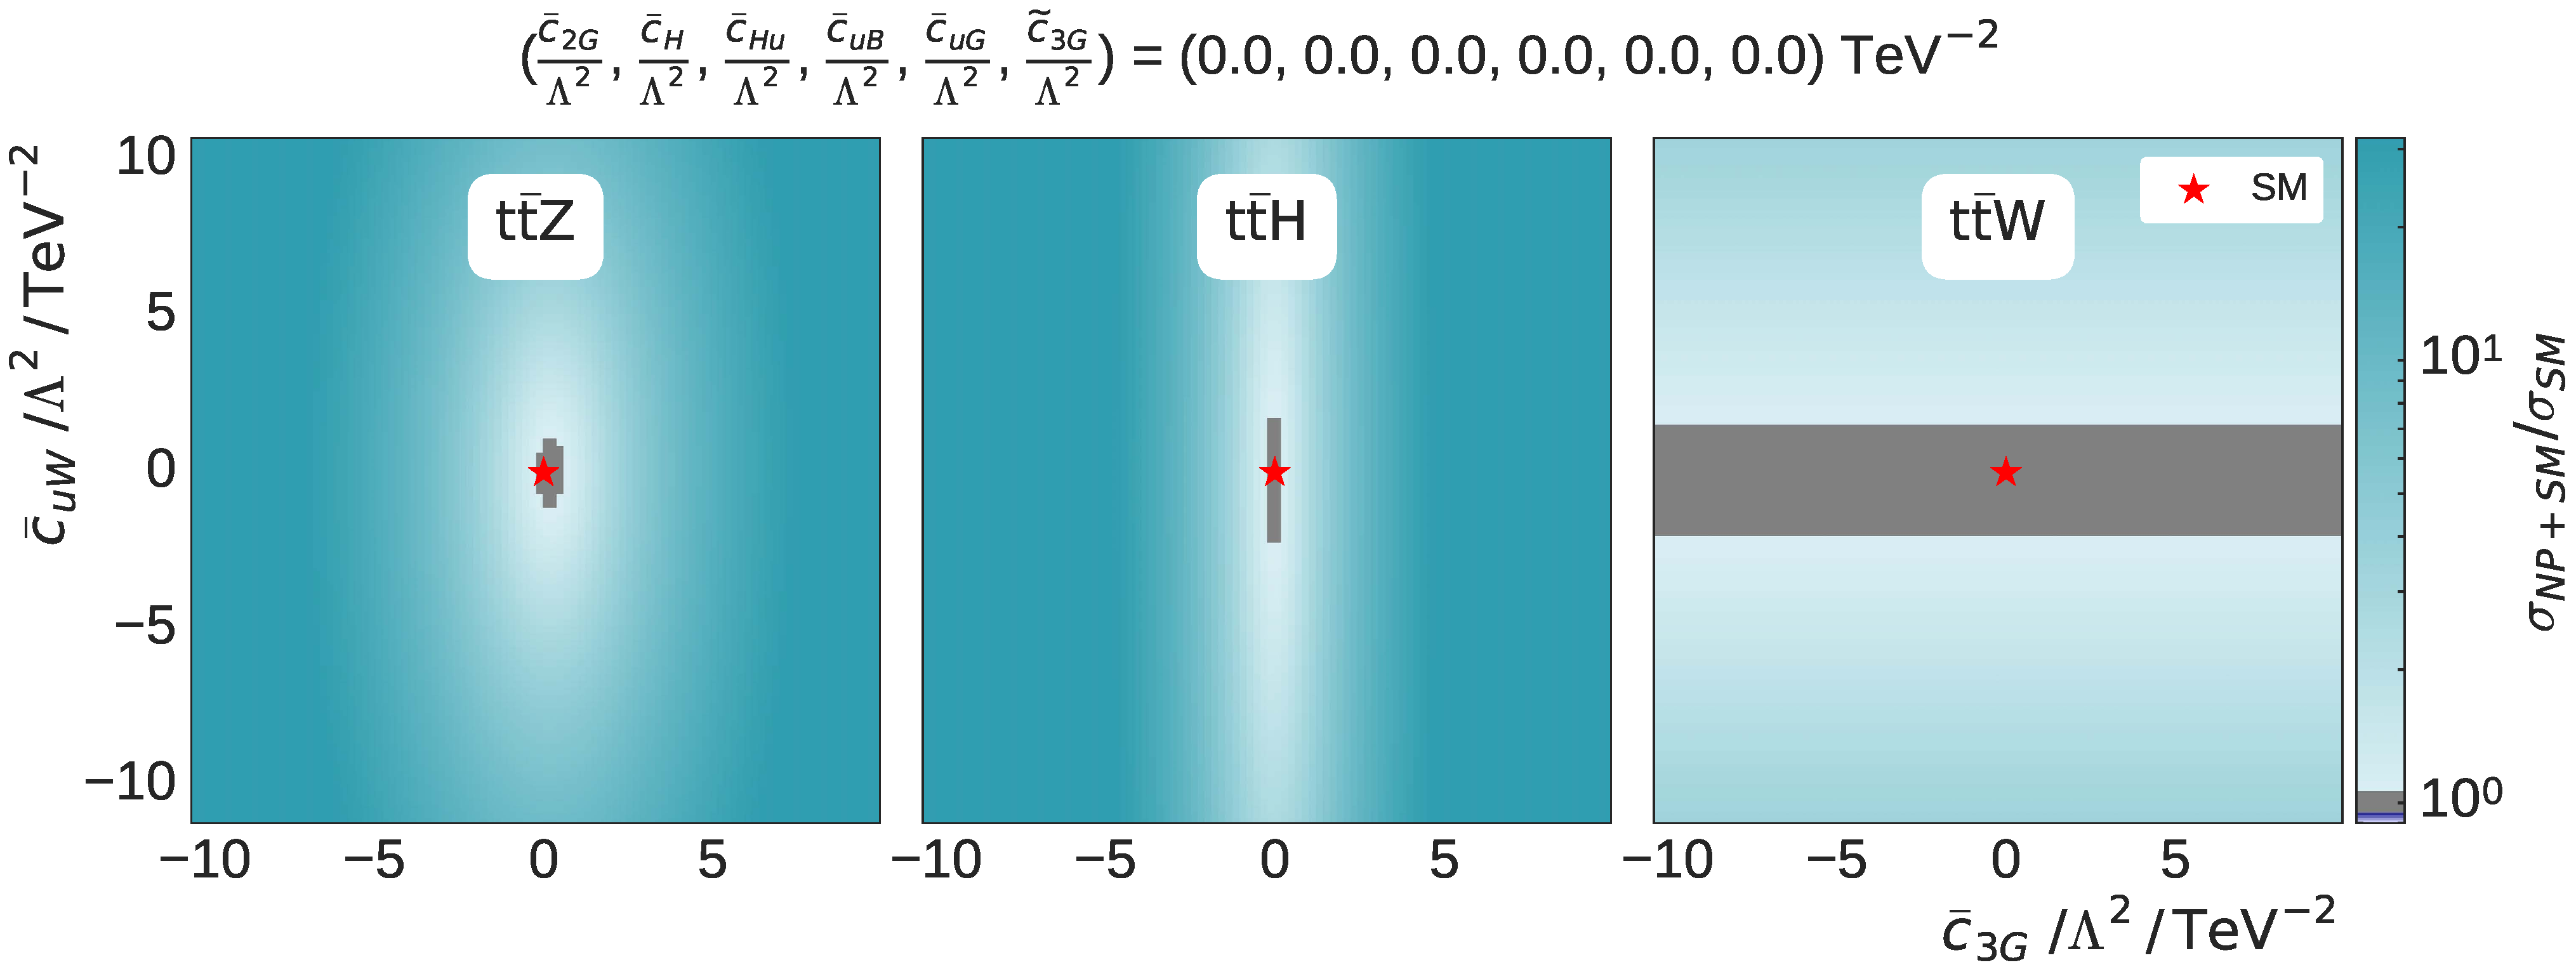
\includegraphics[width=\linewidth]{figures/thirteen-TeV/scaling-frozen/c3G_cuW}
    \caption{}
  \end{subfigure}
  \begin{subfigure}{\linewidth}
    \centering
    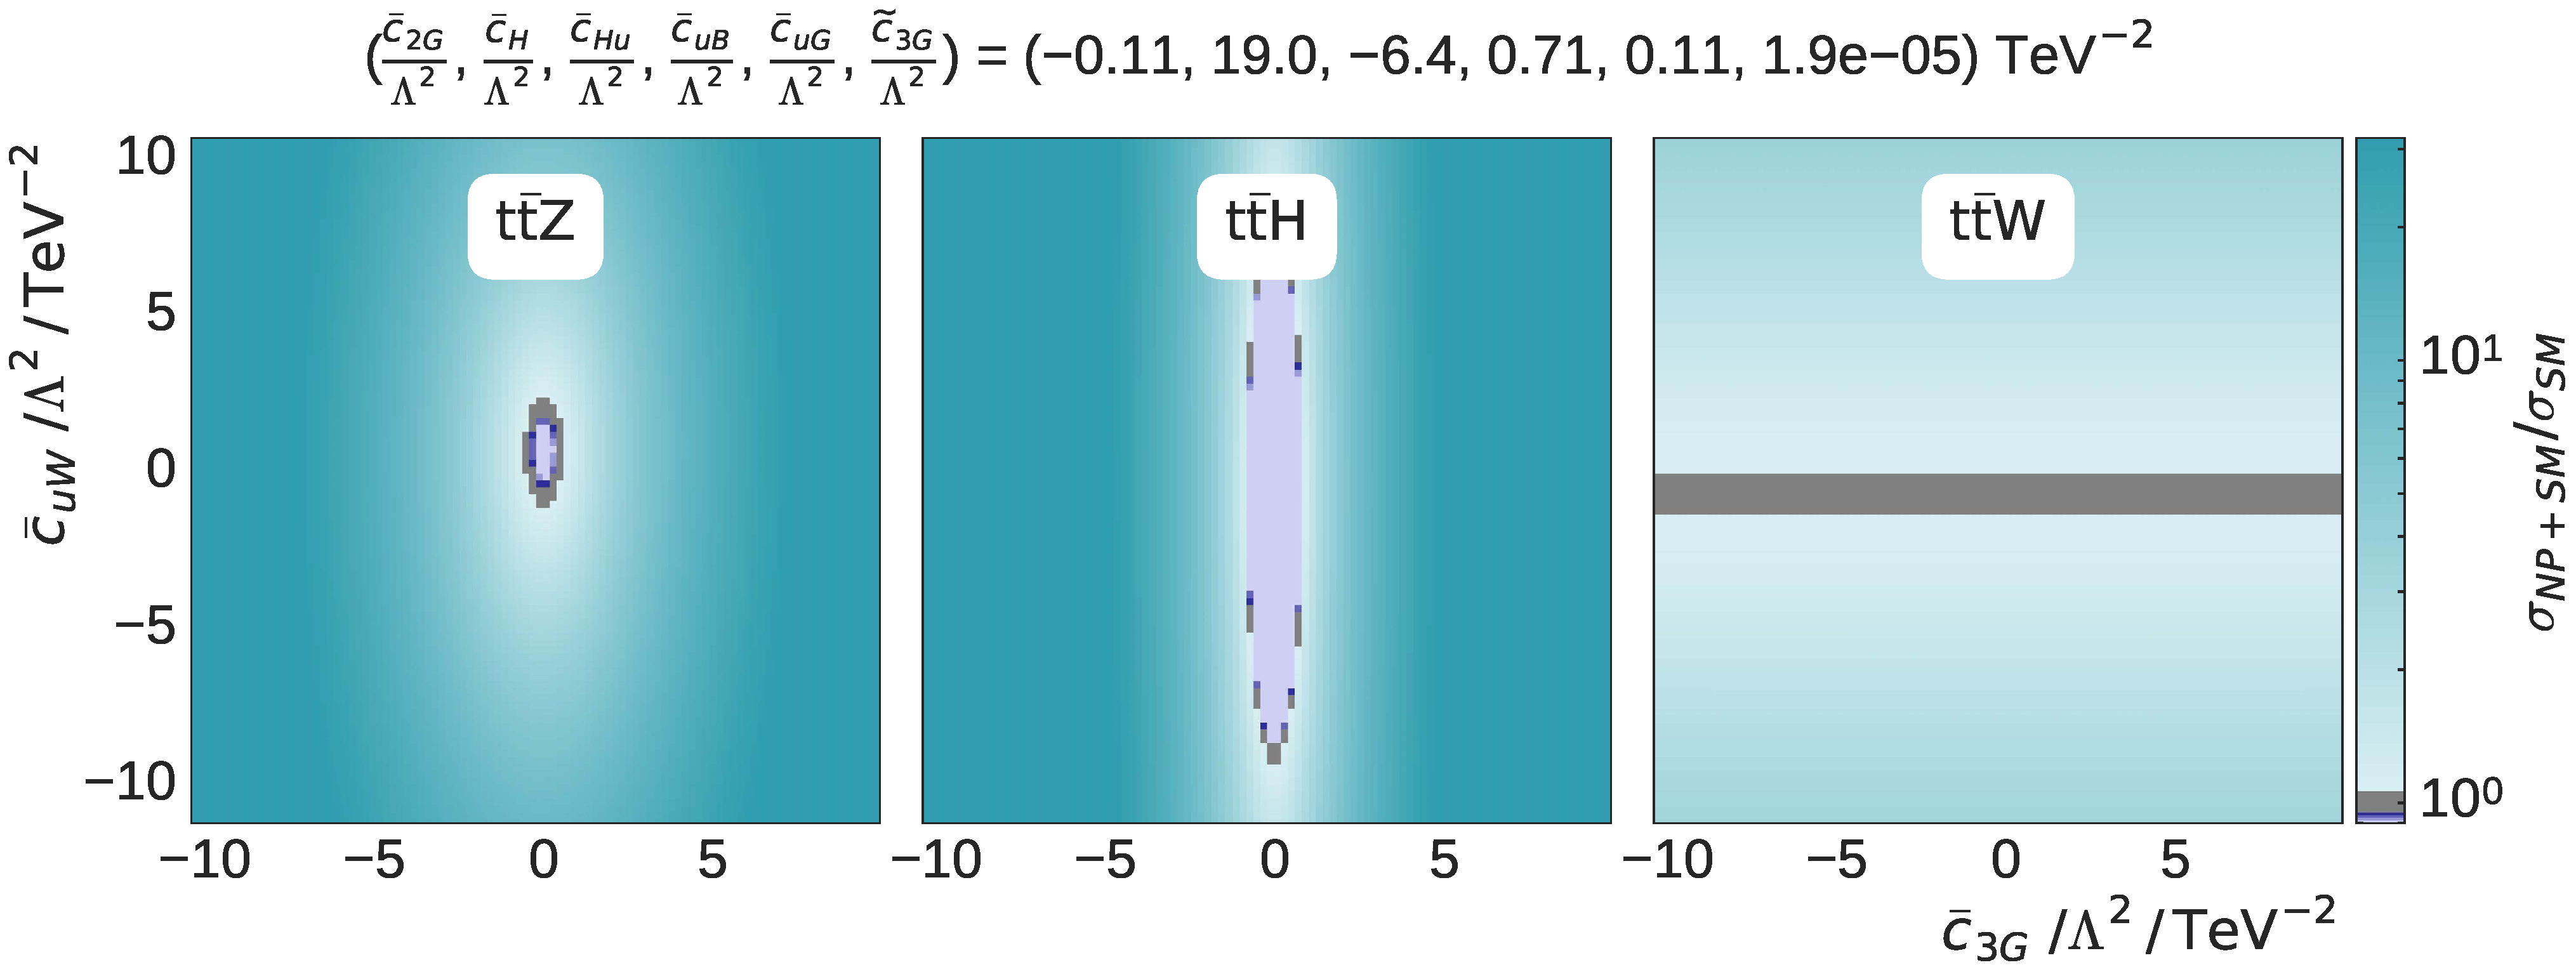
\includegraphics[width=\linewidth]{figures/thirteen-TeV/scaling/c3G_cuW}
    \caption{}
  \end{subfigure}
  \begin{subfigure}{\linewidth}
    \centering
    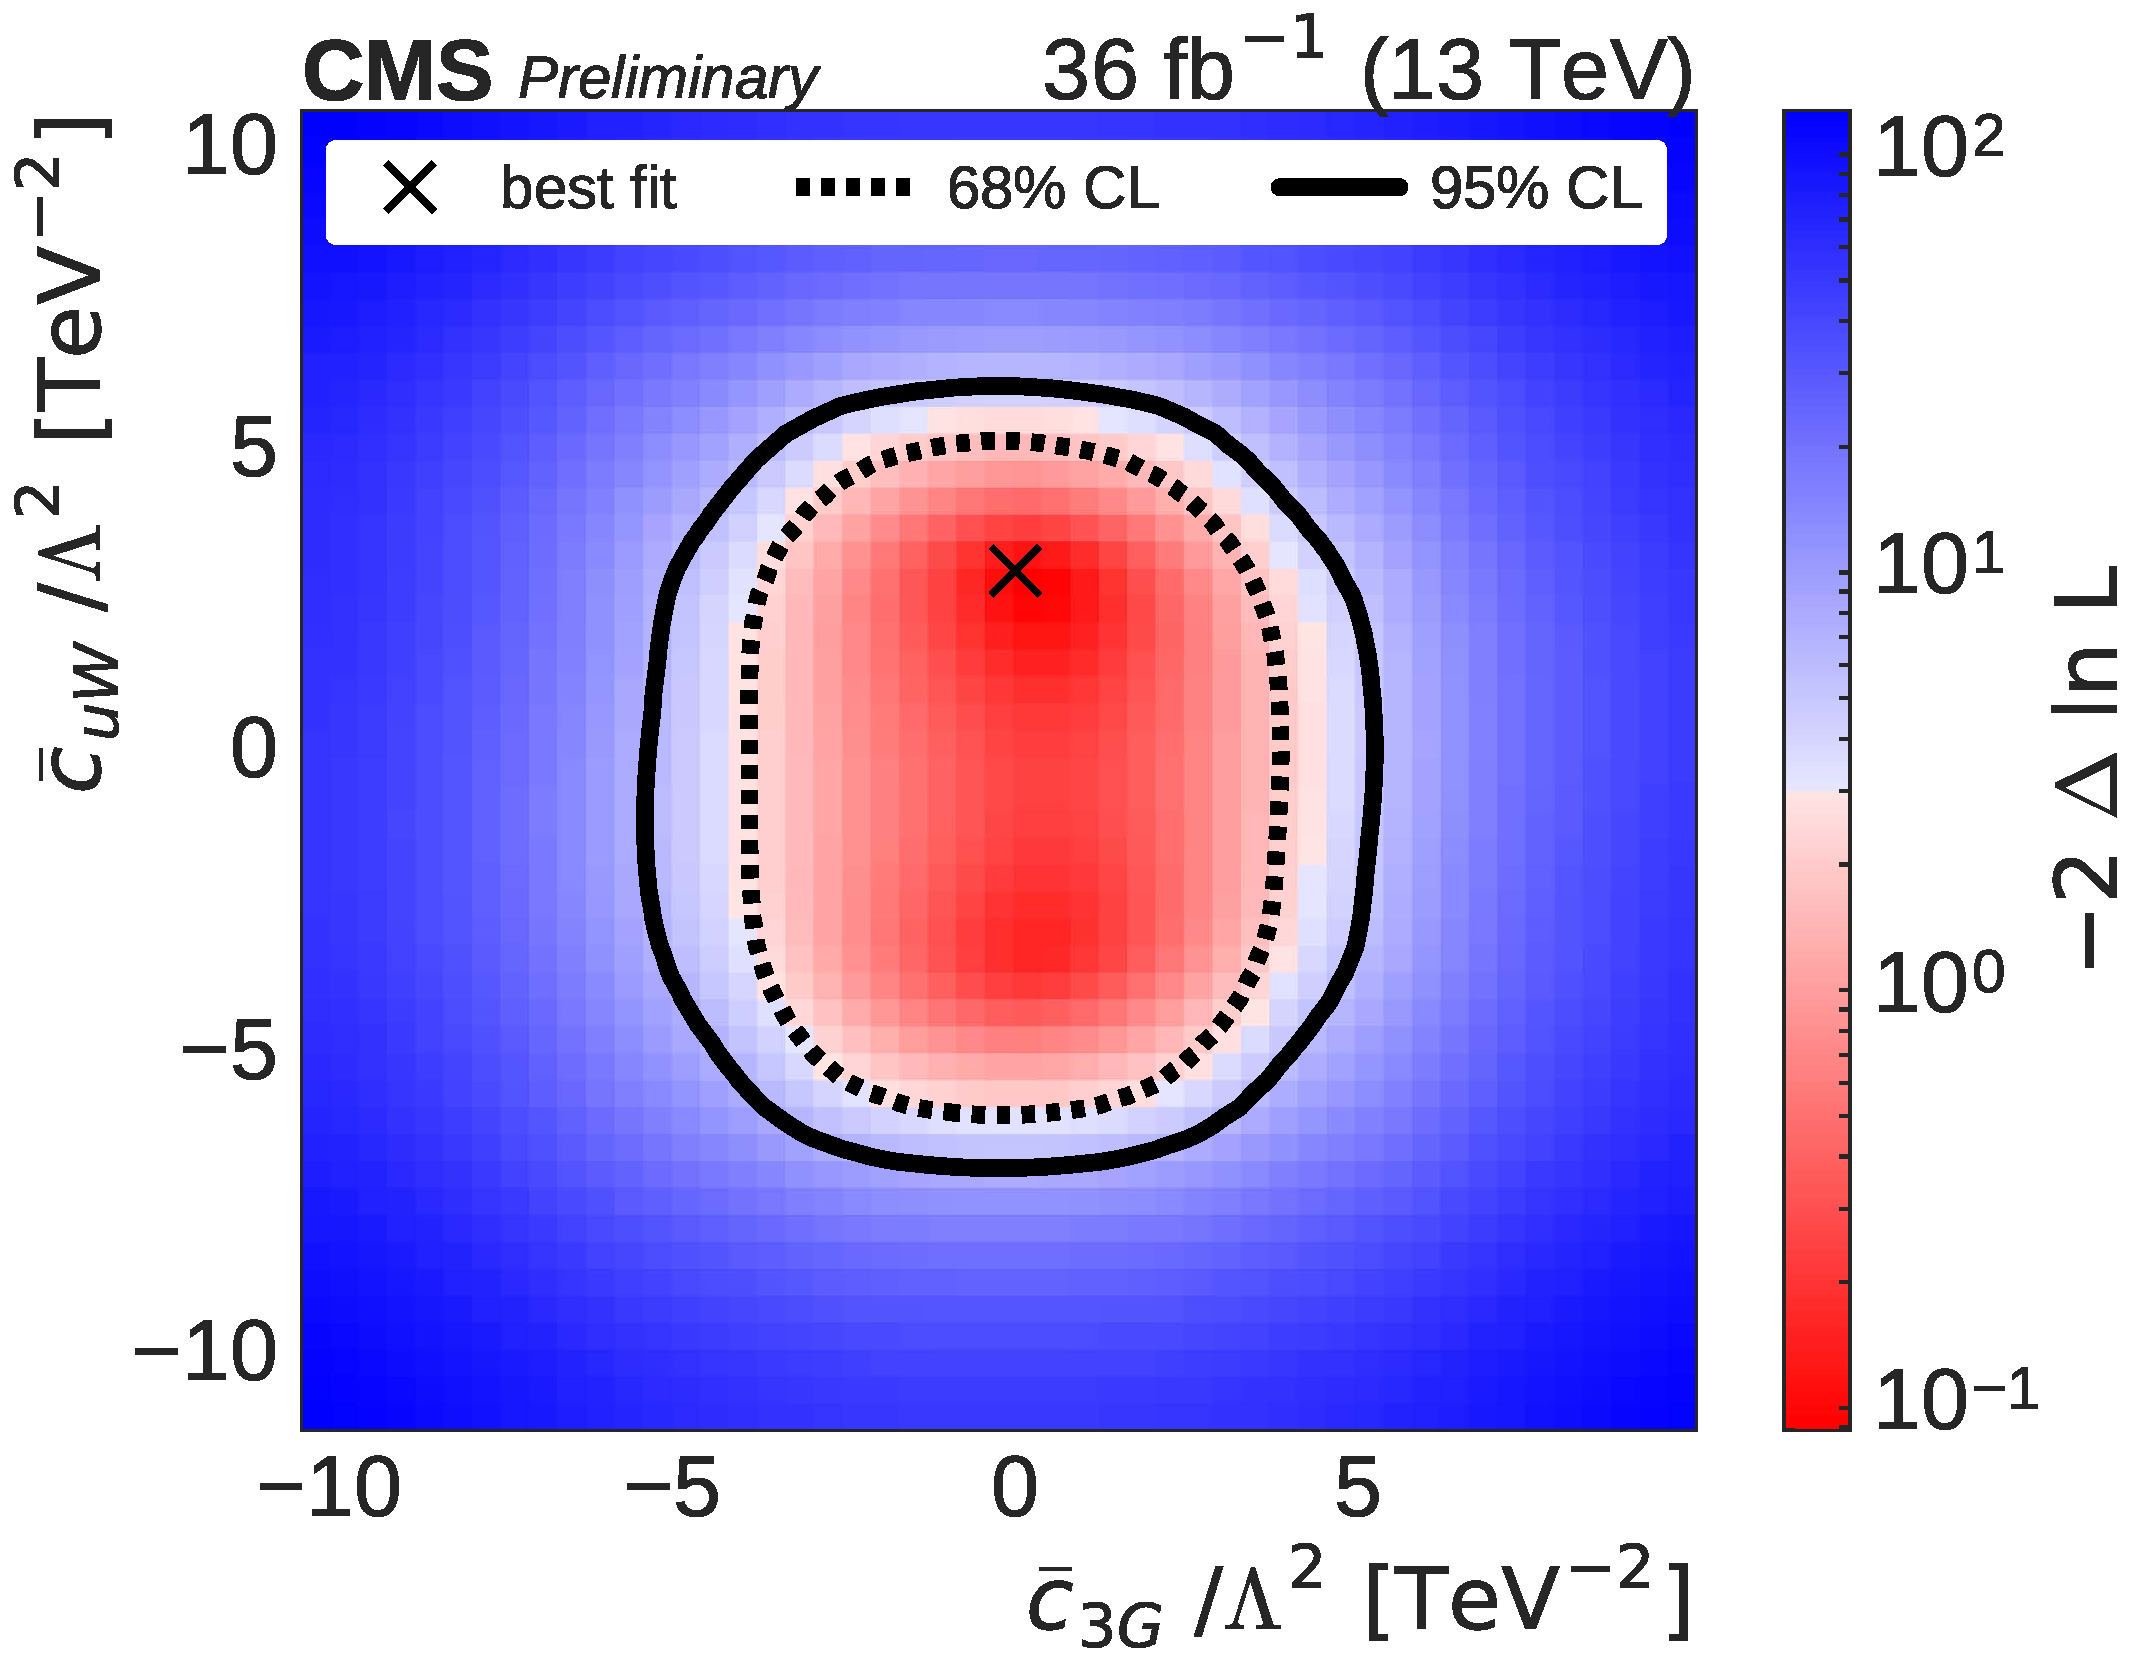
\includegraphics[width=0.6\linewidth]{figures/thirteen-TeV/nll/c3G_cuW}
    \caption{}
  \end{subfigure}
  \vspace{-1cm}
  \setlength{\capwidth}{15cm}
  \caption[Signal scaling and profile likelihood scan in the \cthreeG, \cuW plane]{Signal scaling
  shown in the \cthreeG, \cuW plane with all other coefficients fixed to zero (a) or their best-fit
  values (b) for \ttZ (left), \ttH (center), and \ttW (right). The color represents the scaling
  ($\sigma_\text{NP + SM} / \sigma_\text{SM}$) due to NP effects. The star represents the SM point in
  which all $c_i=0$. The negative log likelihood is shown in (c). The best fit is represented by a
  cross. The \SI{68}{\percent} and \SI{95}{\percent} CL contours are shown with dashed and solid
  lines, respectively.}
\end{figure}

\begin{figure}
  \vspace{-1cm}
  \begin{subfigure}{\linewidth}
    \centering
    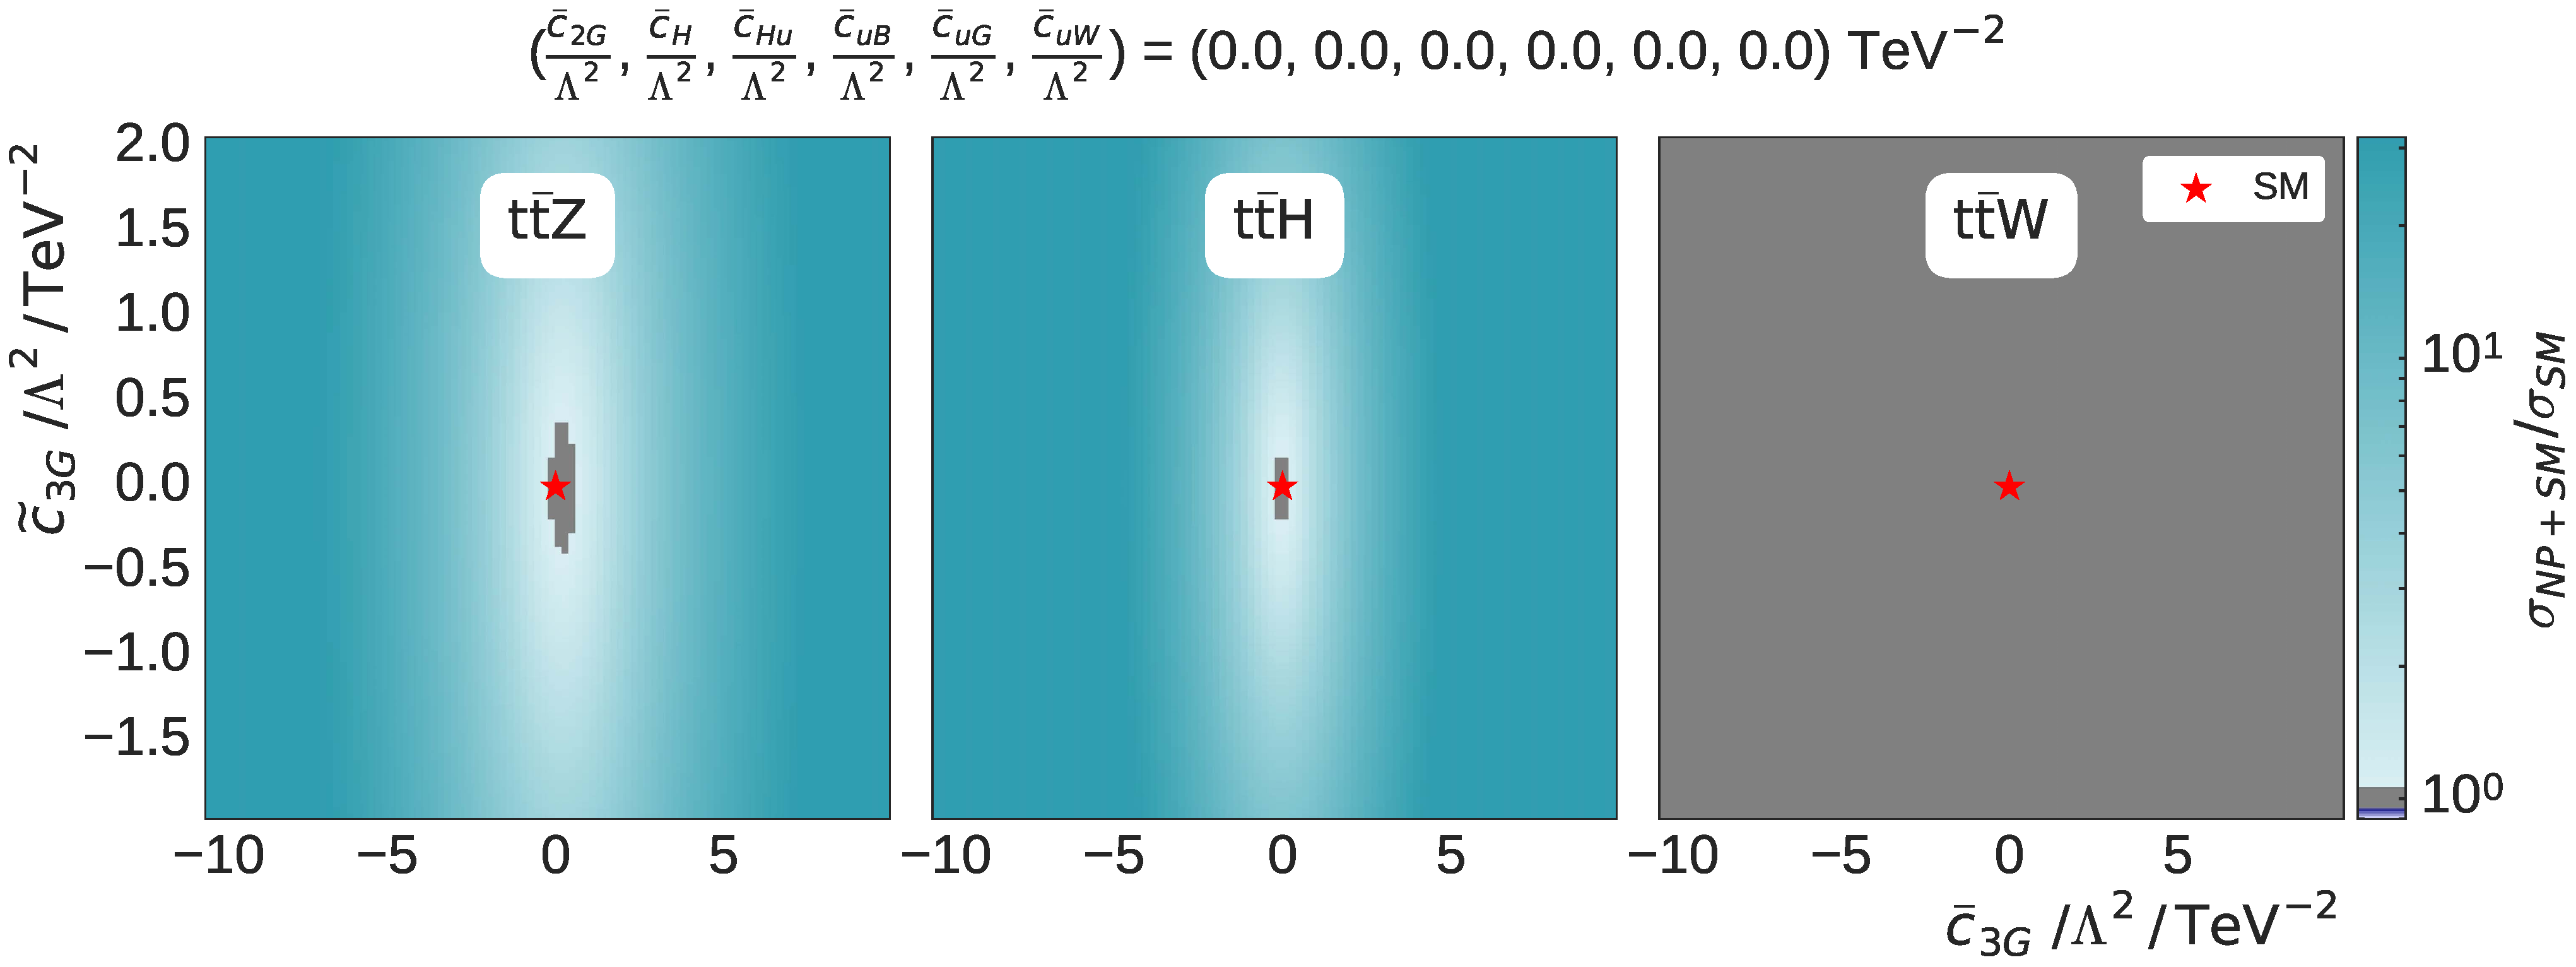
\includegraphics[width=\linewidth]{figures/thirteen-TeV/scaling-frozen/c3G_tc3G}
    \caption{}
  \end{subfigure}
  \begin{subfigure}{\linewidth}
    \centering
    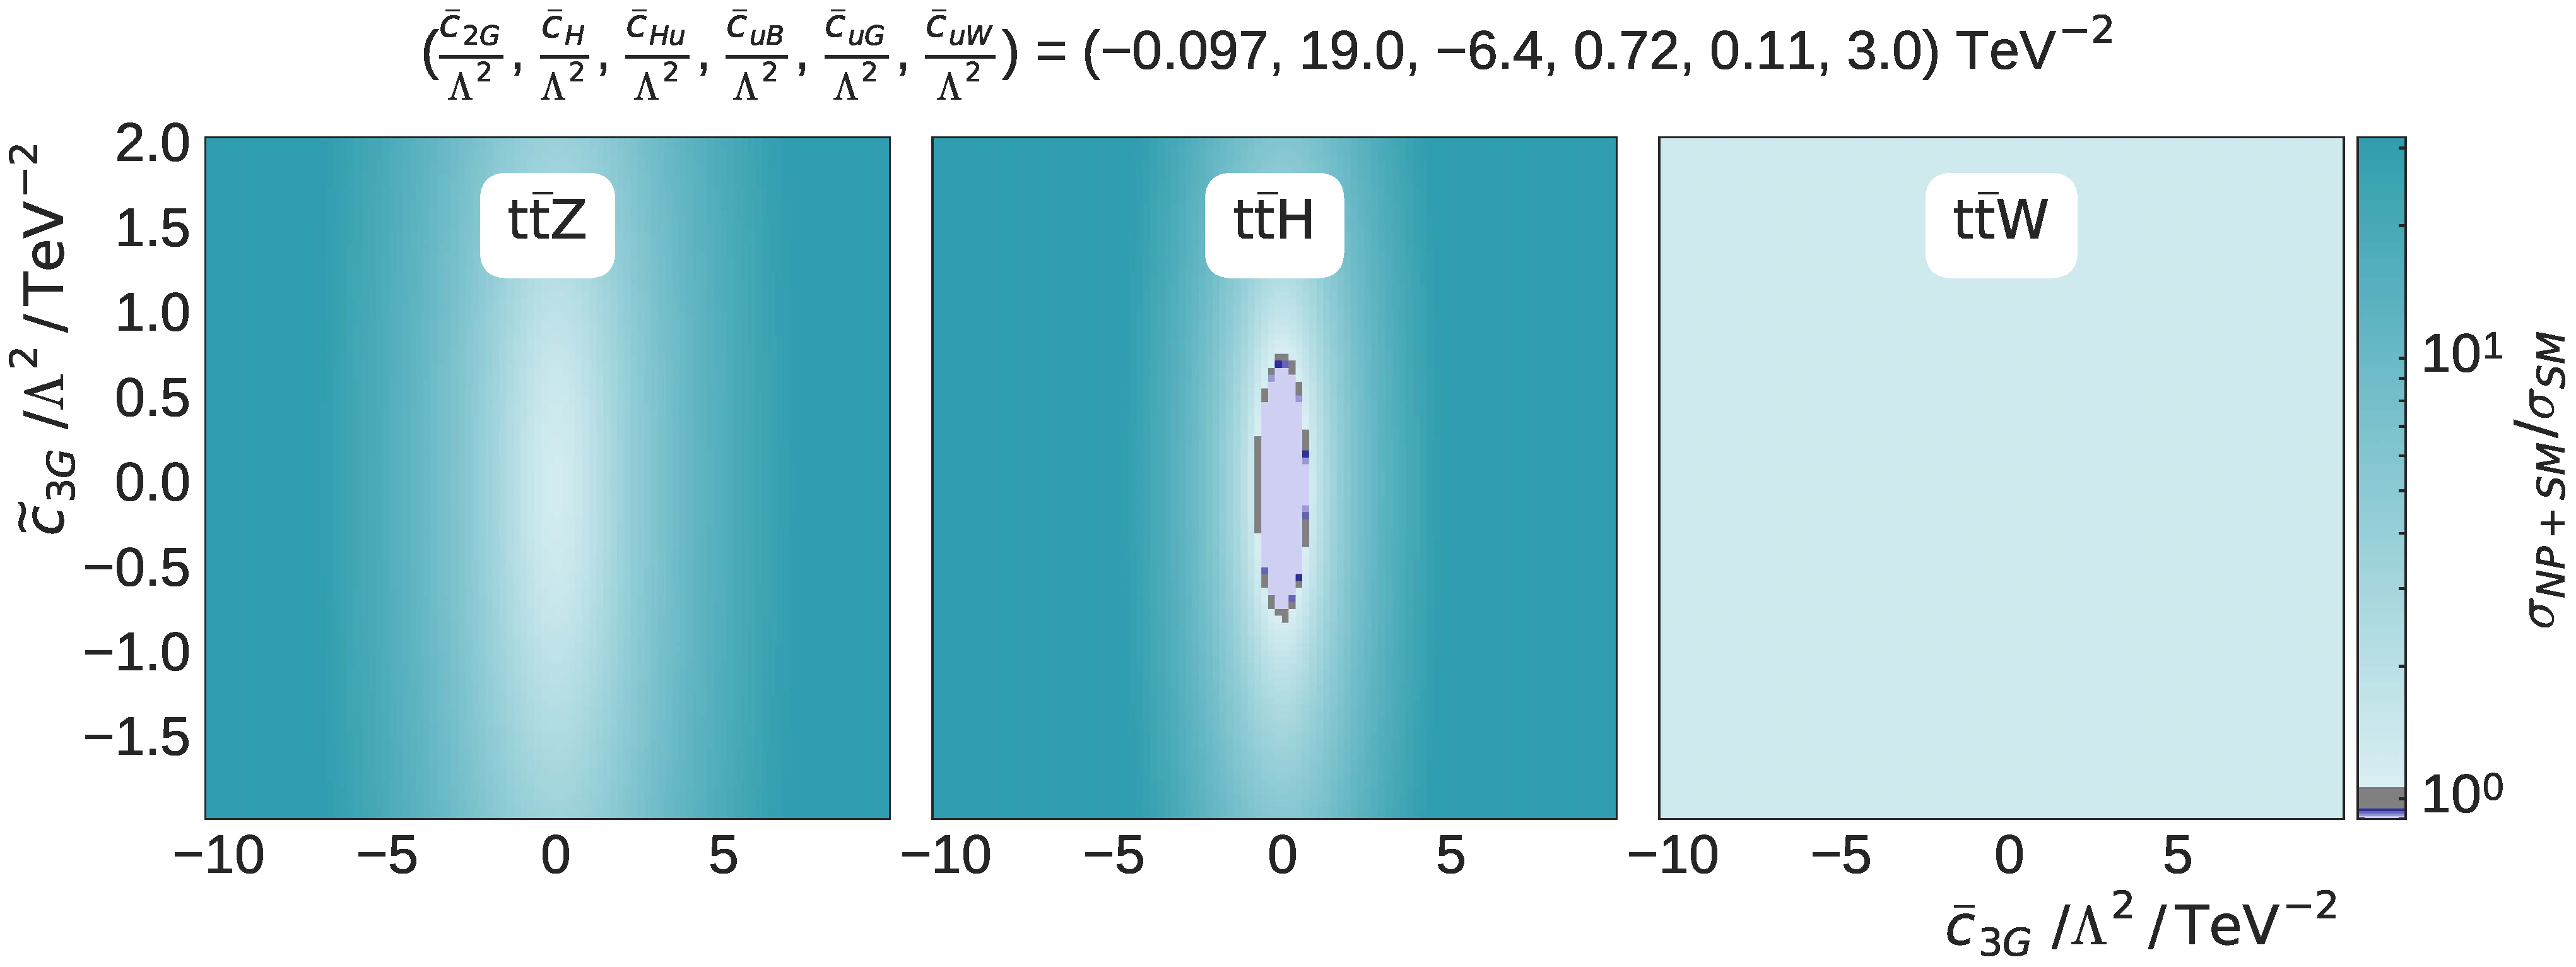
\includegraphics[width=\linewidth]{figures/thirteen-TeV/scaling/c3G_tc3G}
    \caption{}
  \end{subfigure}
  \begin{subfigure}{\linewidth}
    \centering
    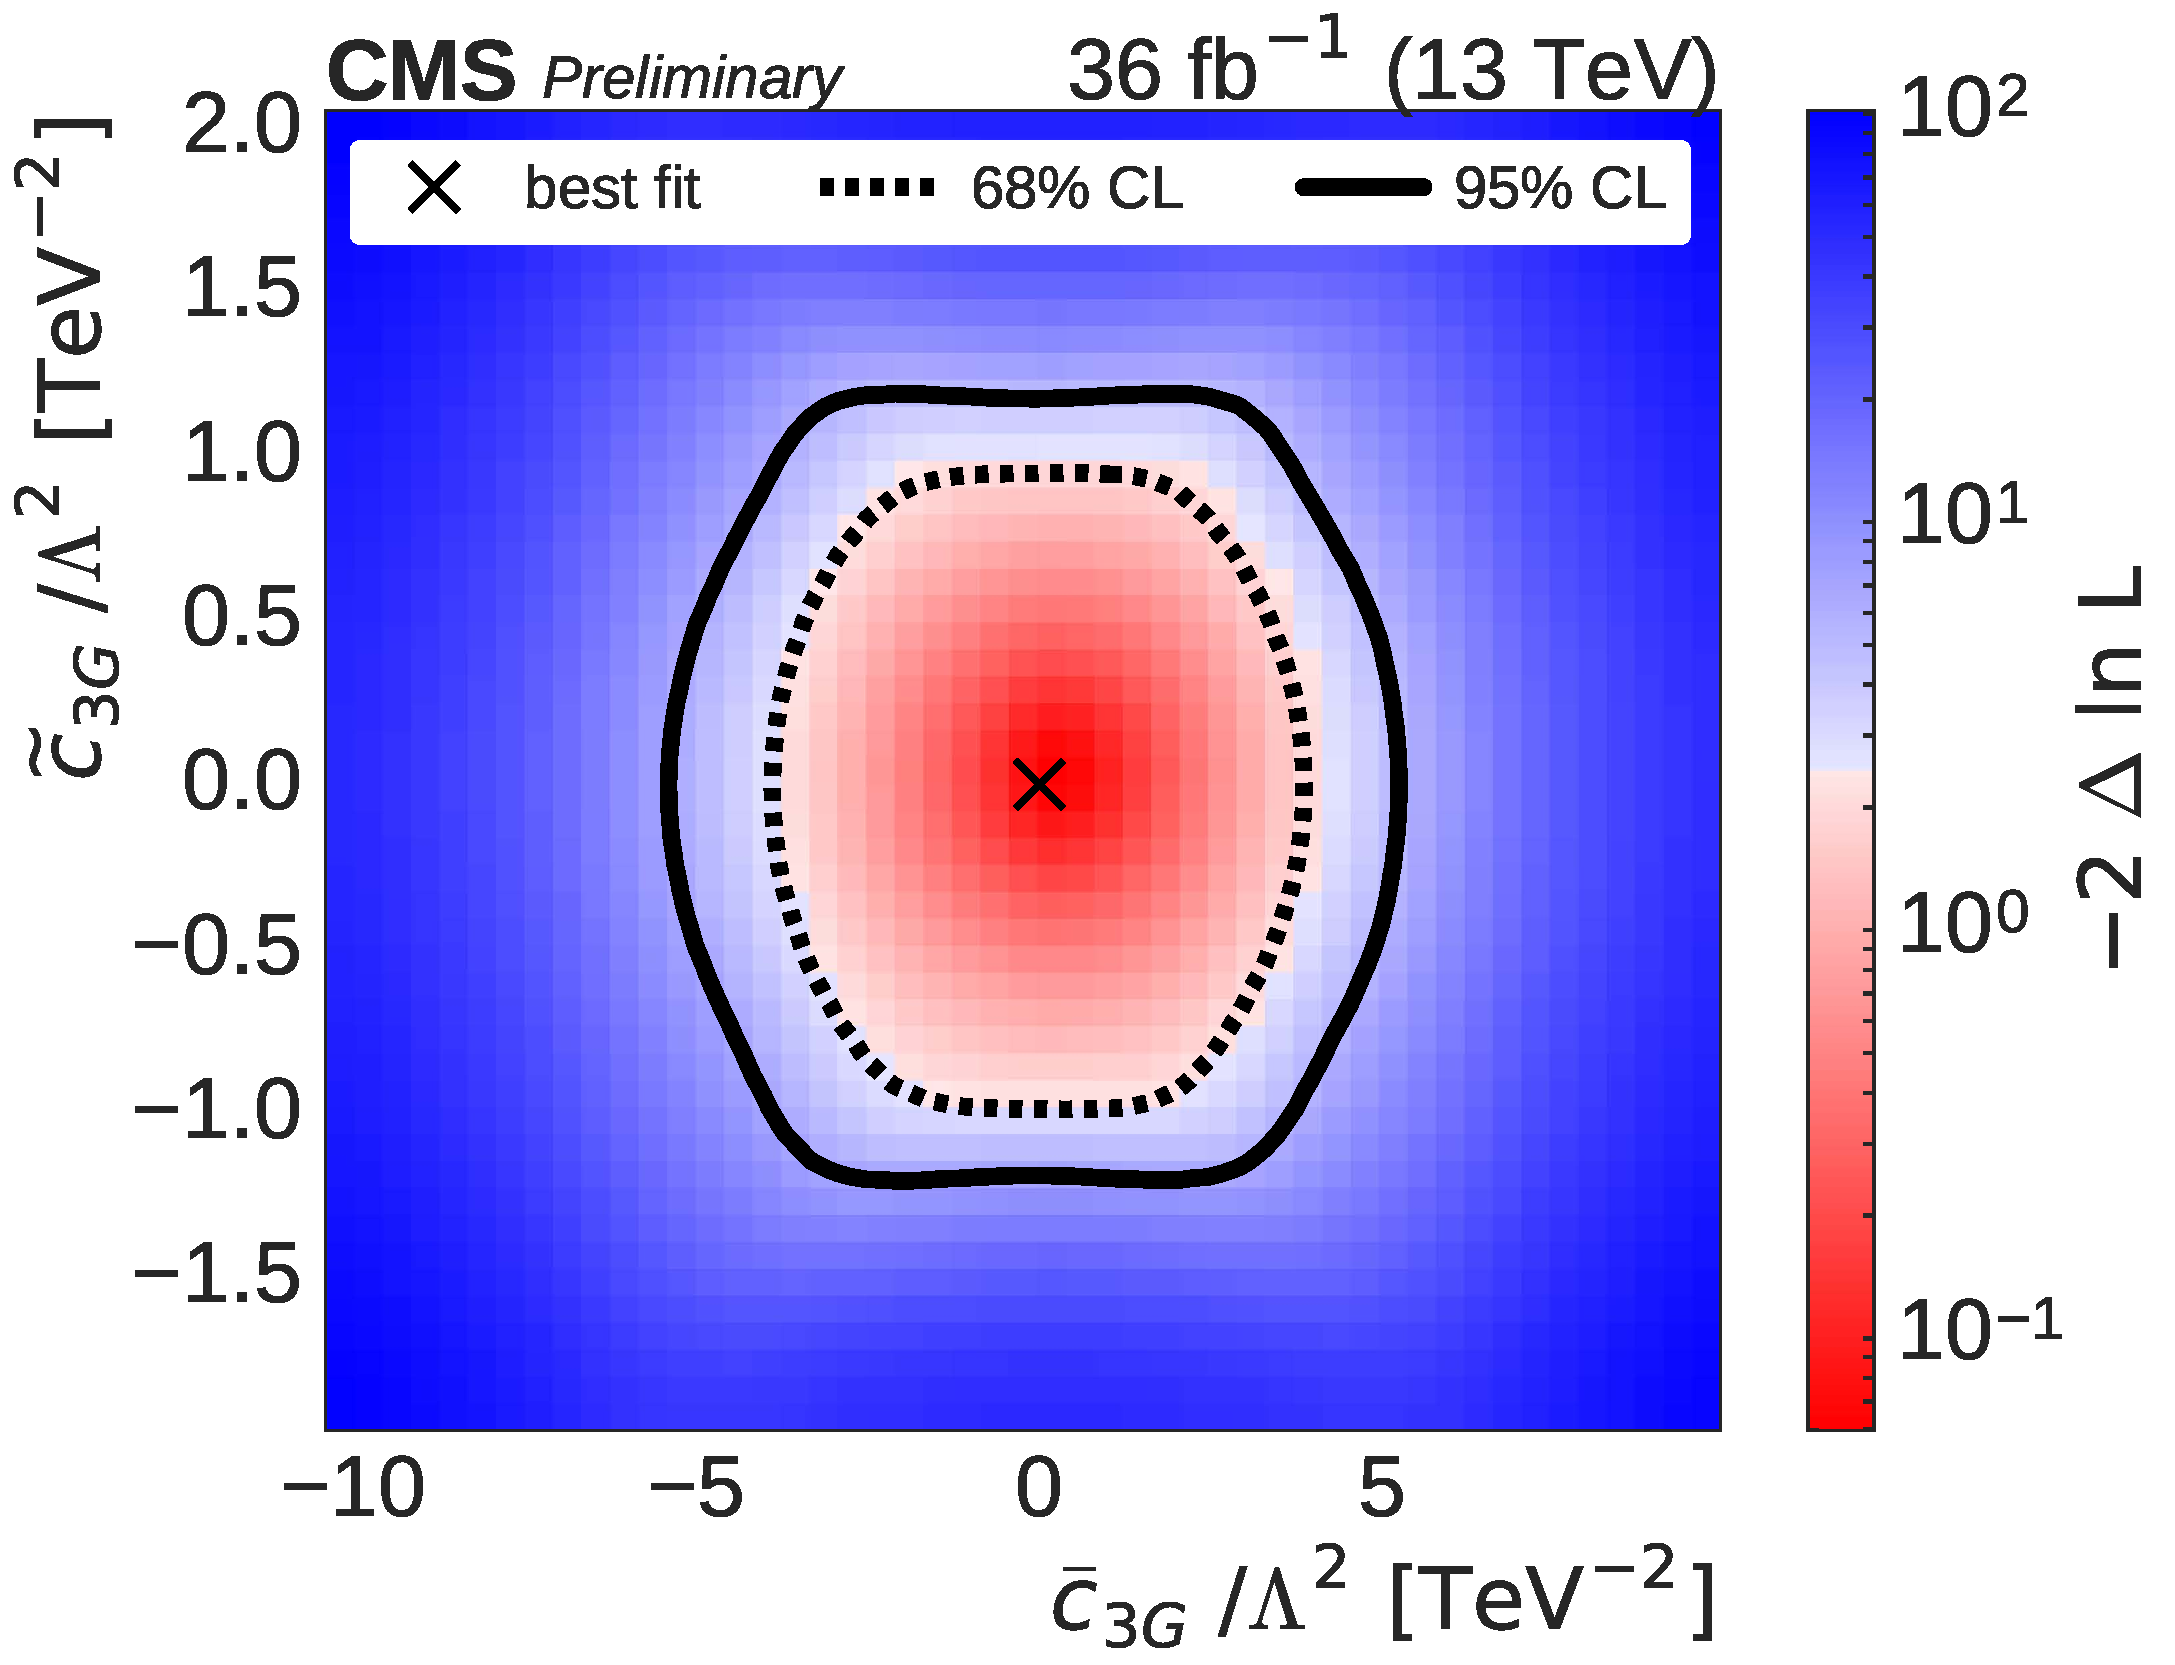
\includegraphics[width=0.6\linewidth]{figures/thirteen-TeV/nll/c3G_tc3G}
    \caption{}
  \end{subfigure}
  \vspace{-1cm}
  \setlength{\capwidth}{15cm}
  \caption[Signal scaling and profile likelihood scan in the \cthreeG, \tcthreeG plane]{Signal scaling shown in the \cthreeG, \tcthreeG plane with all other coefficients fixed to zero (a) or their best-fit values (b) for \ttZ (left), \ttH (center), and \ttW (right). The color represents the scaling ($\sigma_\text{NP + SM} / \sigma_\text{SM}$) due to NP effects. The star represents the SM point in which all $c_i=0$. The negative log likelihood is shown in (c). The best fit is represented by a cross. The \SI{68}{\percent} and \SI{95}{\percent} CL contours are shown with dashed and solid lines, respectively.}
\end{figure}

\begin{figure}
  \vspace{-1cm}
  \begin{subfigure}{\linewidth}
    \centering
    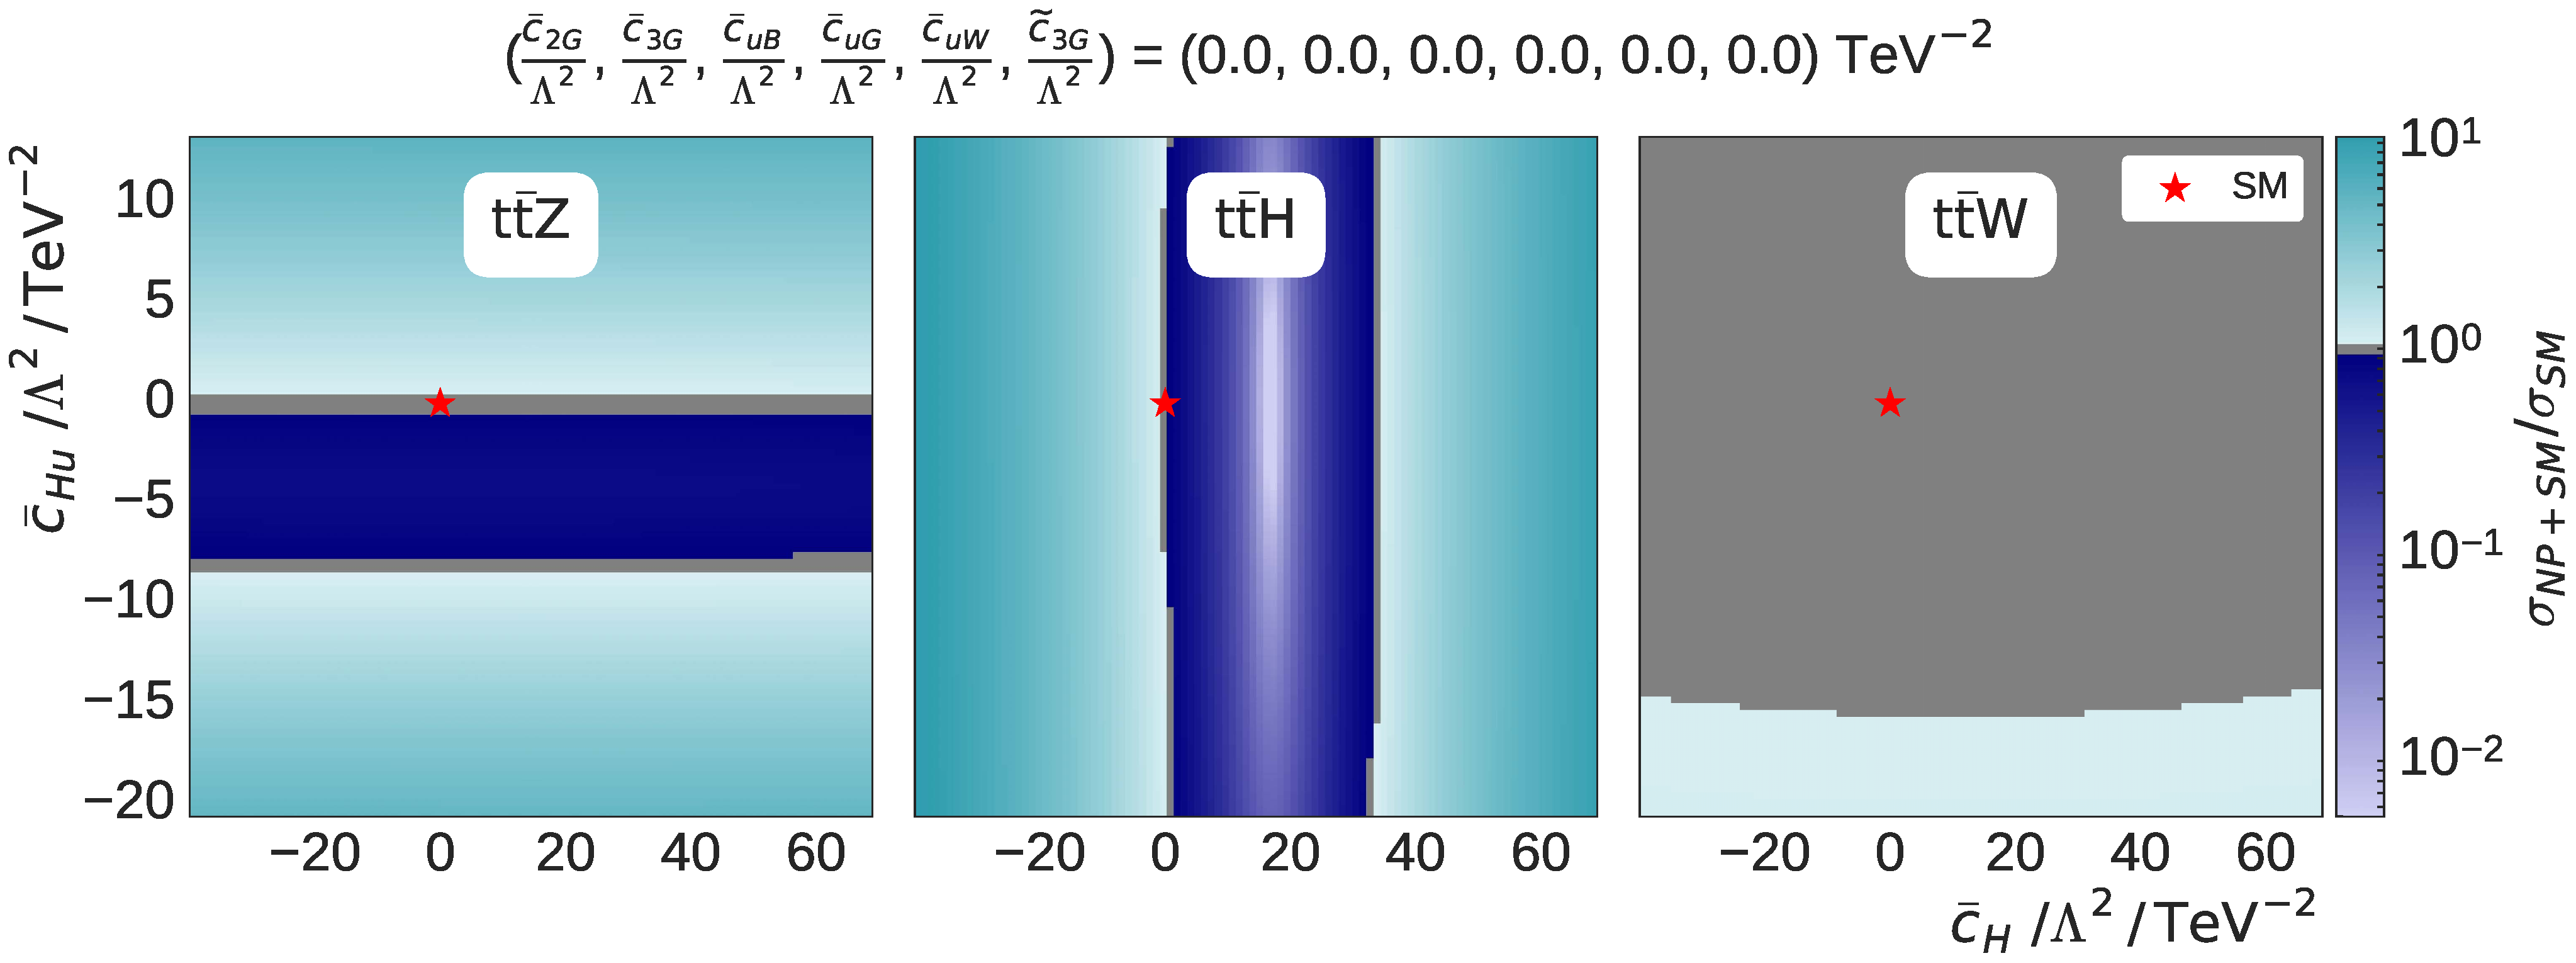
\includegraphics[width=\linewidth]{figures/thirteen-TeV/scaling-frozen/cH_cHu}
    \caption{}
  \end{subfigure}
  \begin{subfigure}{\linewidth}
    \centering
    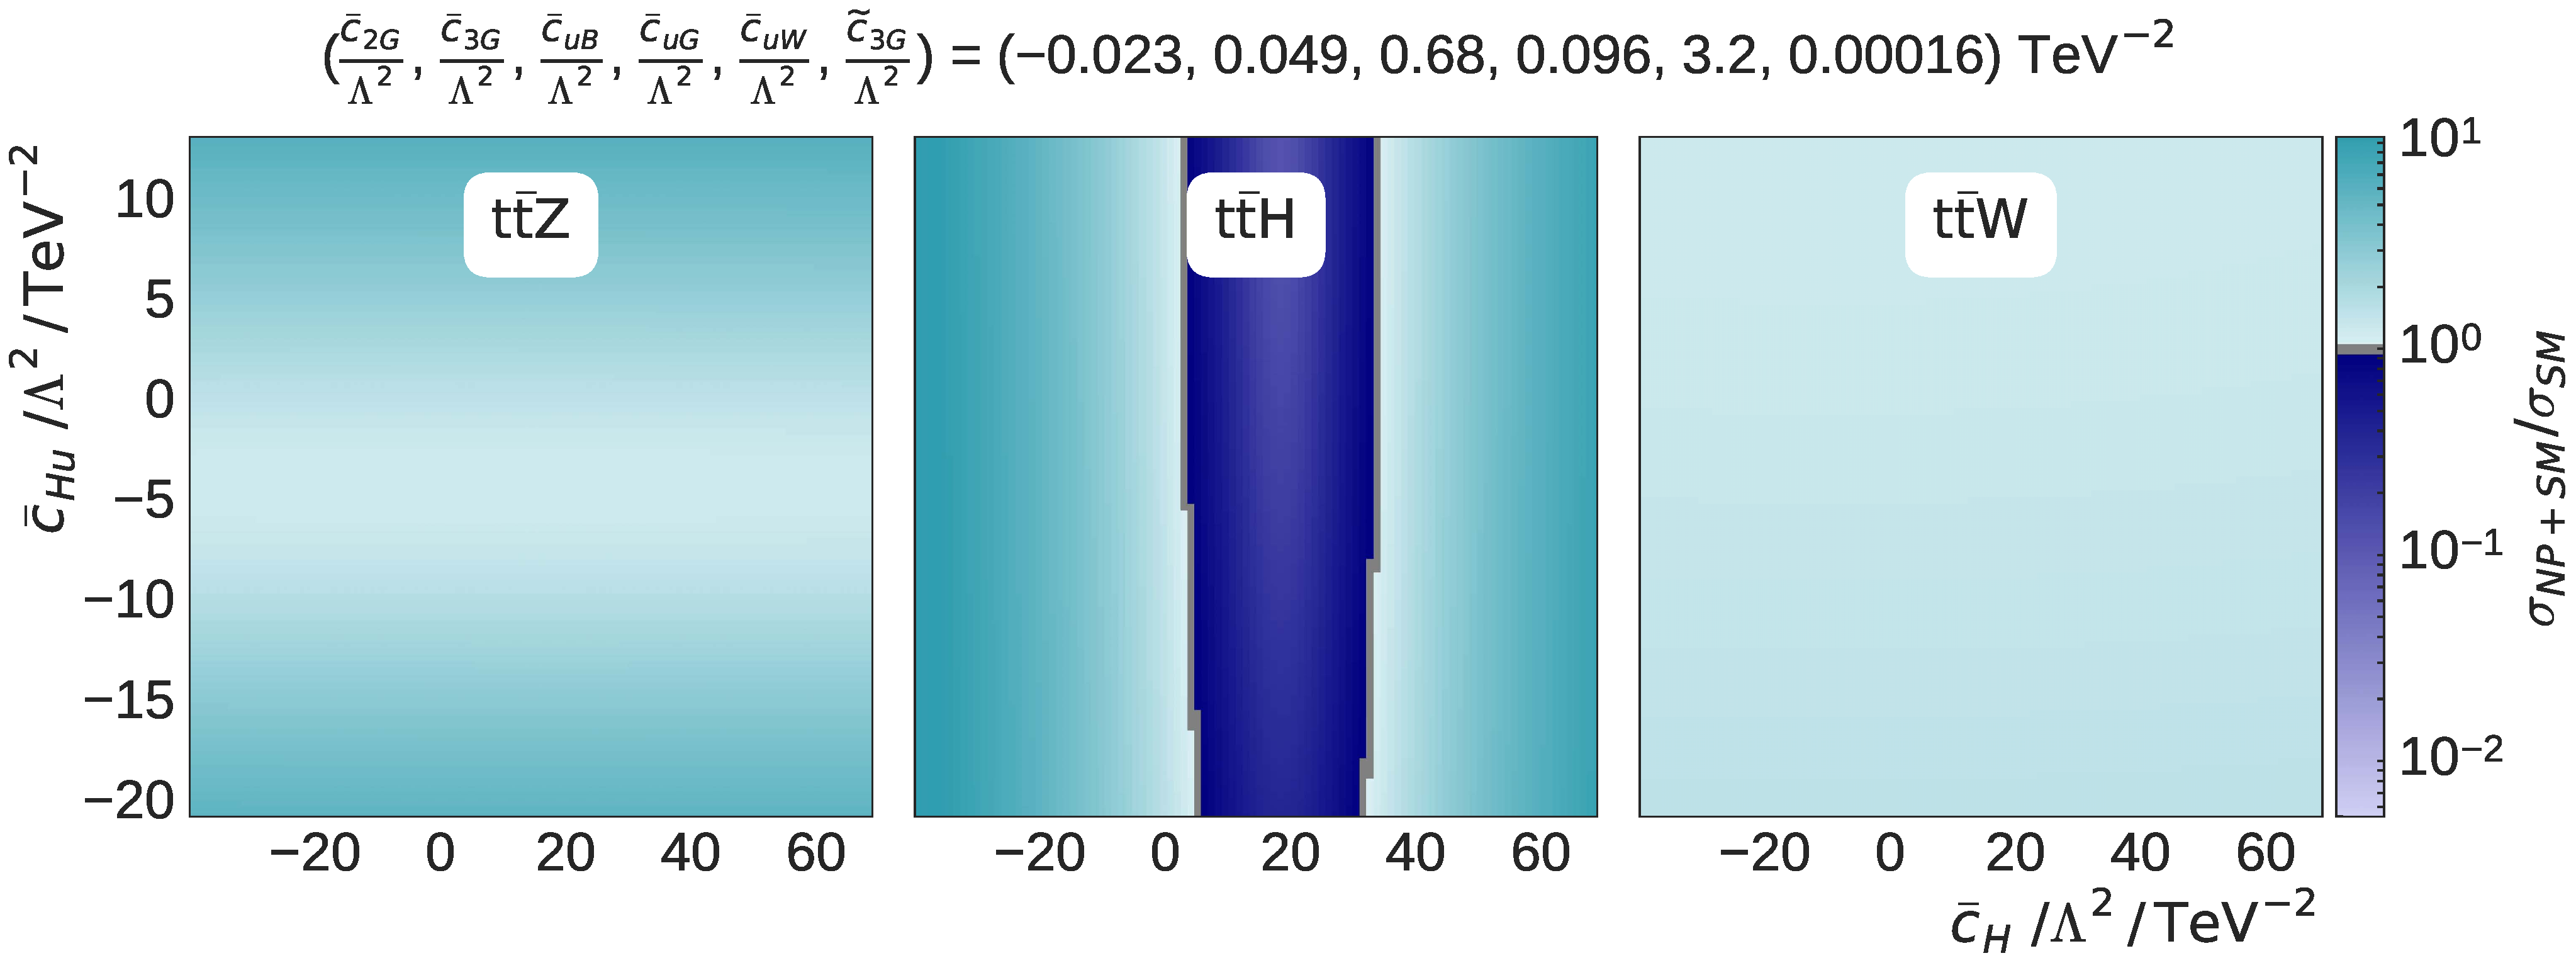
\includegraphics[width=\linewidth]{figures/thirteen-TeV/scaling/cH_cHu}
    \caption{}
  \end{subfigure}
  \begin{subfigure}{\linewidth}
    \centering
    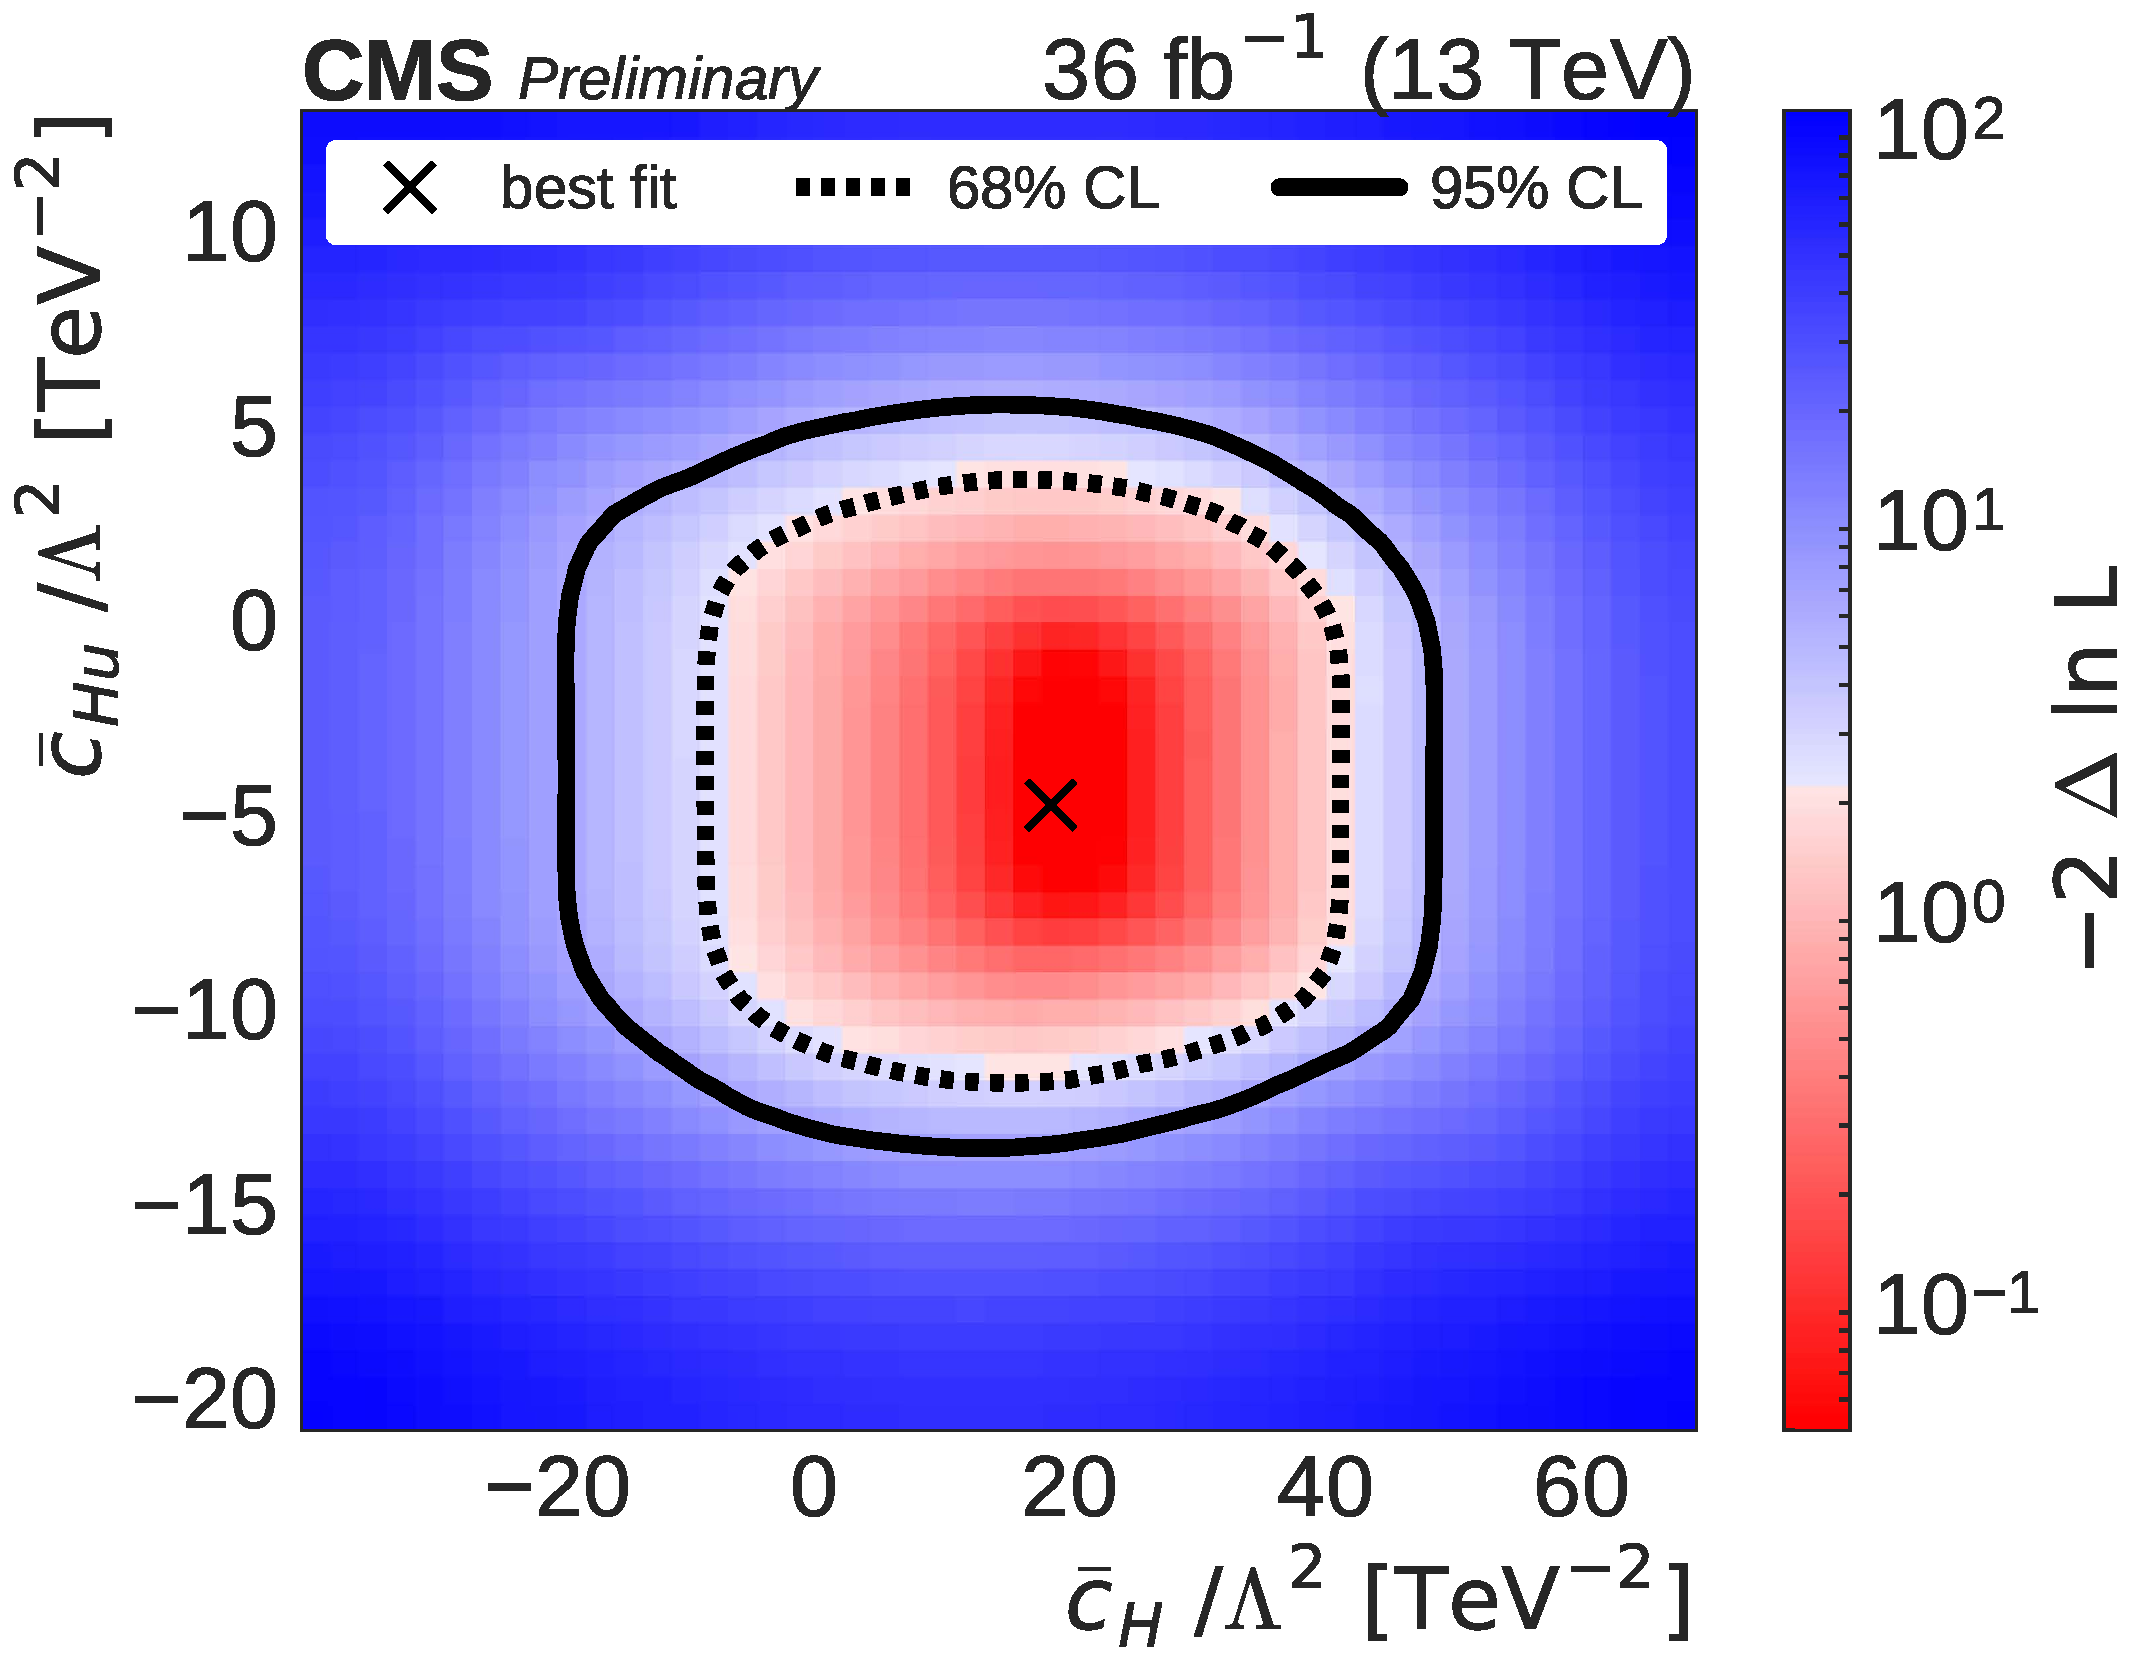
\includegraphics[width=0.6\linewidth]{figures/thirteen-TeV/nll/cH_cHu}
    \caption{}
  \end{subfigure}
  \vspace{-1cm}
  \setlength{\capwidth}{15cm}
  \caption[Signal scaling and profile likelihood scan in the \cHu, \cH plane]{Signal scaling shown
  in the \cHu, \cH plane with all other coefficients fixed to zero (a) or their best-fit values (b)
  for \ttZ (left), \ttH (center), and \ttW (right). The color represents the scaling ($\sigma_\text{NP
  + SM} / \sigma_\text{SM}$) due to NP effects. The star represents the SM point in which all $c_i=0$.
  The negative log likelihood is shown in (c). The best fit is represented by a cross. The
  \SI{68}{\percent} and \SI{95}{\percent} CL contours are shown with dashed and solid lines,
  respectively.}
\end{figure}

\begin{figure}
  \vspace{-1cm}
  \begin{subfigure}{\linewidth}
    \centering
    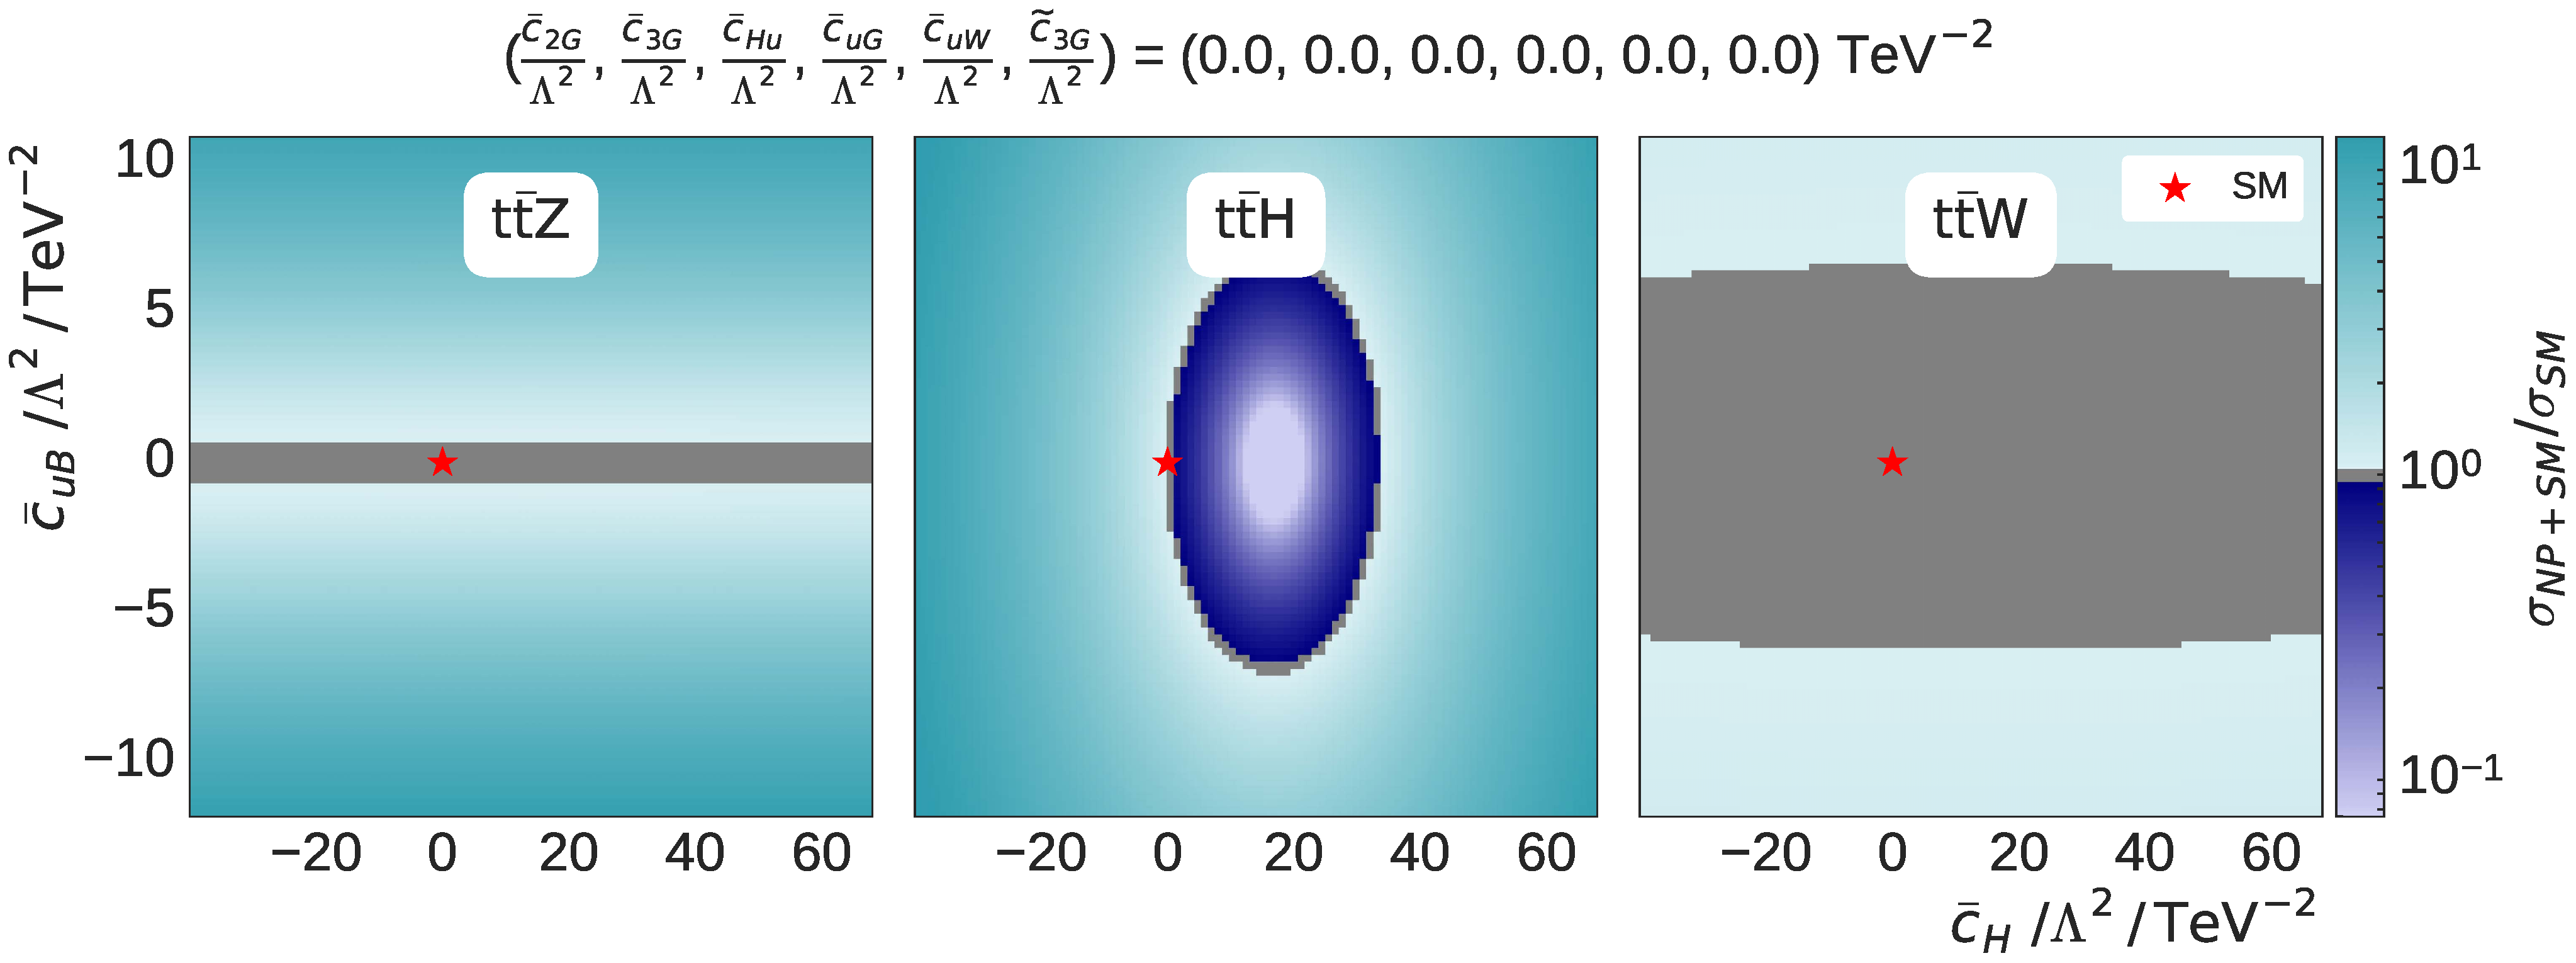
\includegraphics[width=\linewidth]{figures/thirteen-TeV/scaling-frozen/cH_cuB}
    \caption{}
  \end{subfigure}
  \begin{subfigure}{\linewidth}
    \centering
    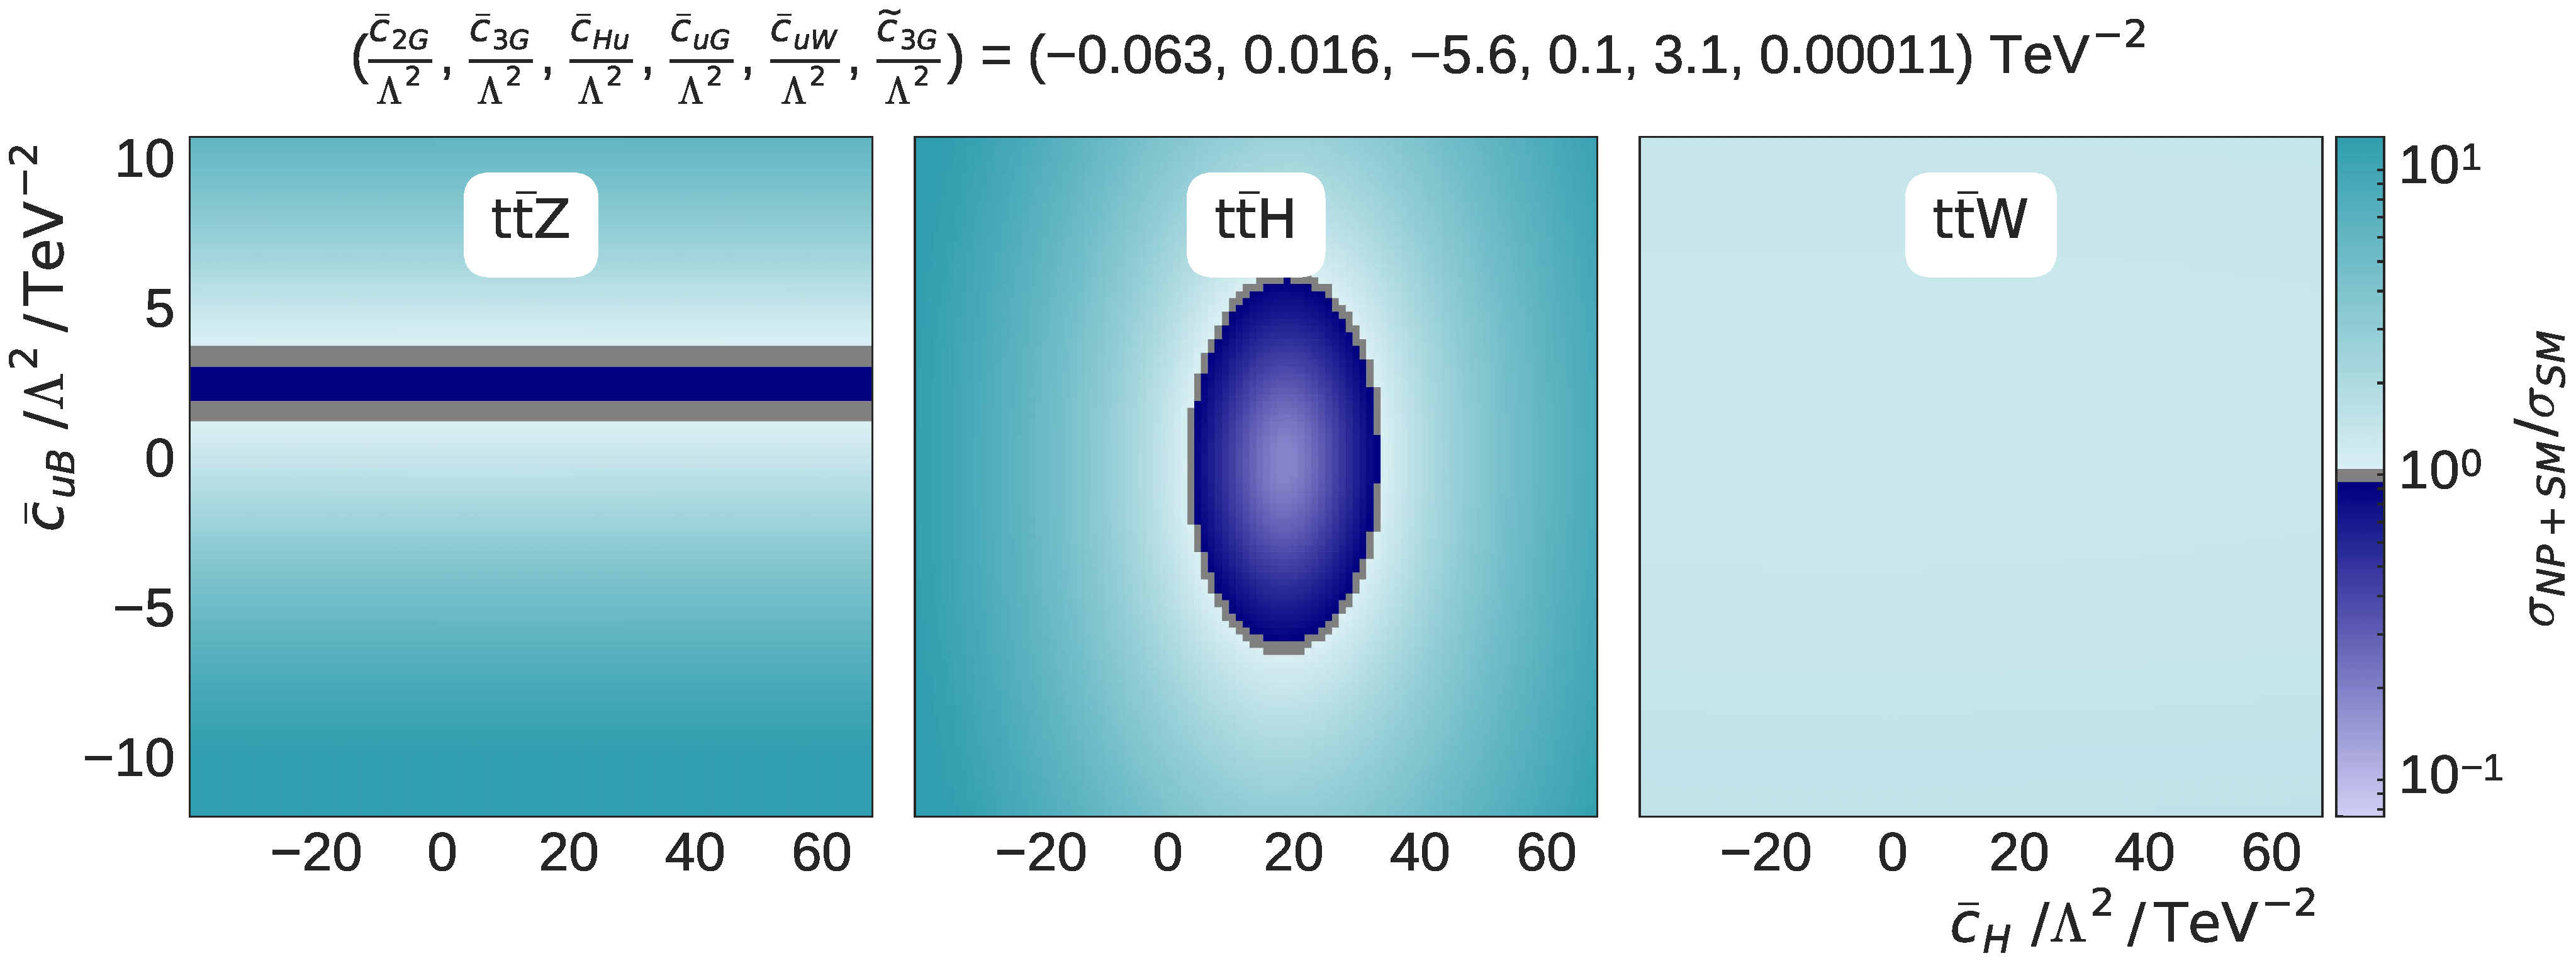
\includegraphics[width=\linewidth]{figures/thirteen-TeV/scaling/cH_cuB}
    \caption{}
  \end{subfigure}
  \begin{subfigure}{\linewidth}
    \centering
    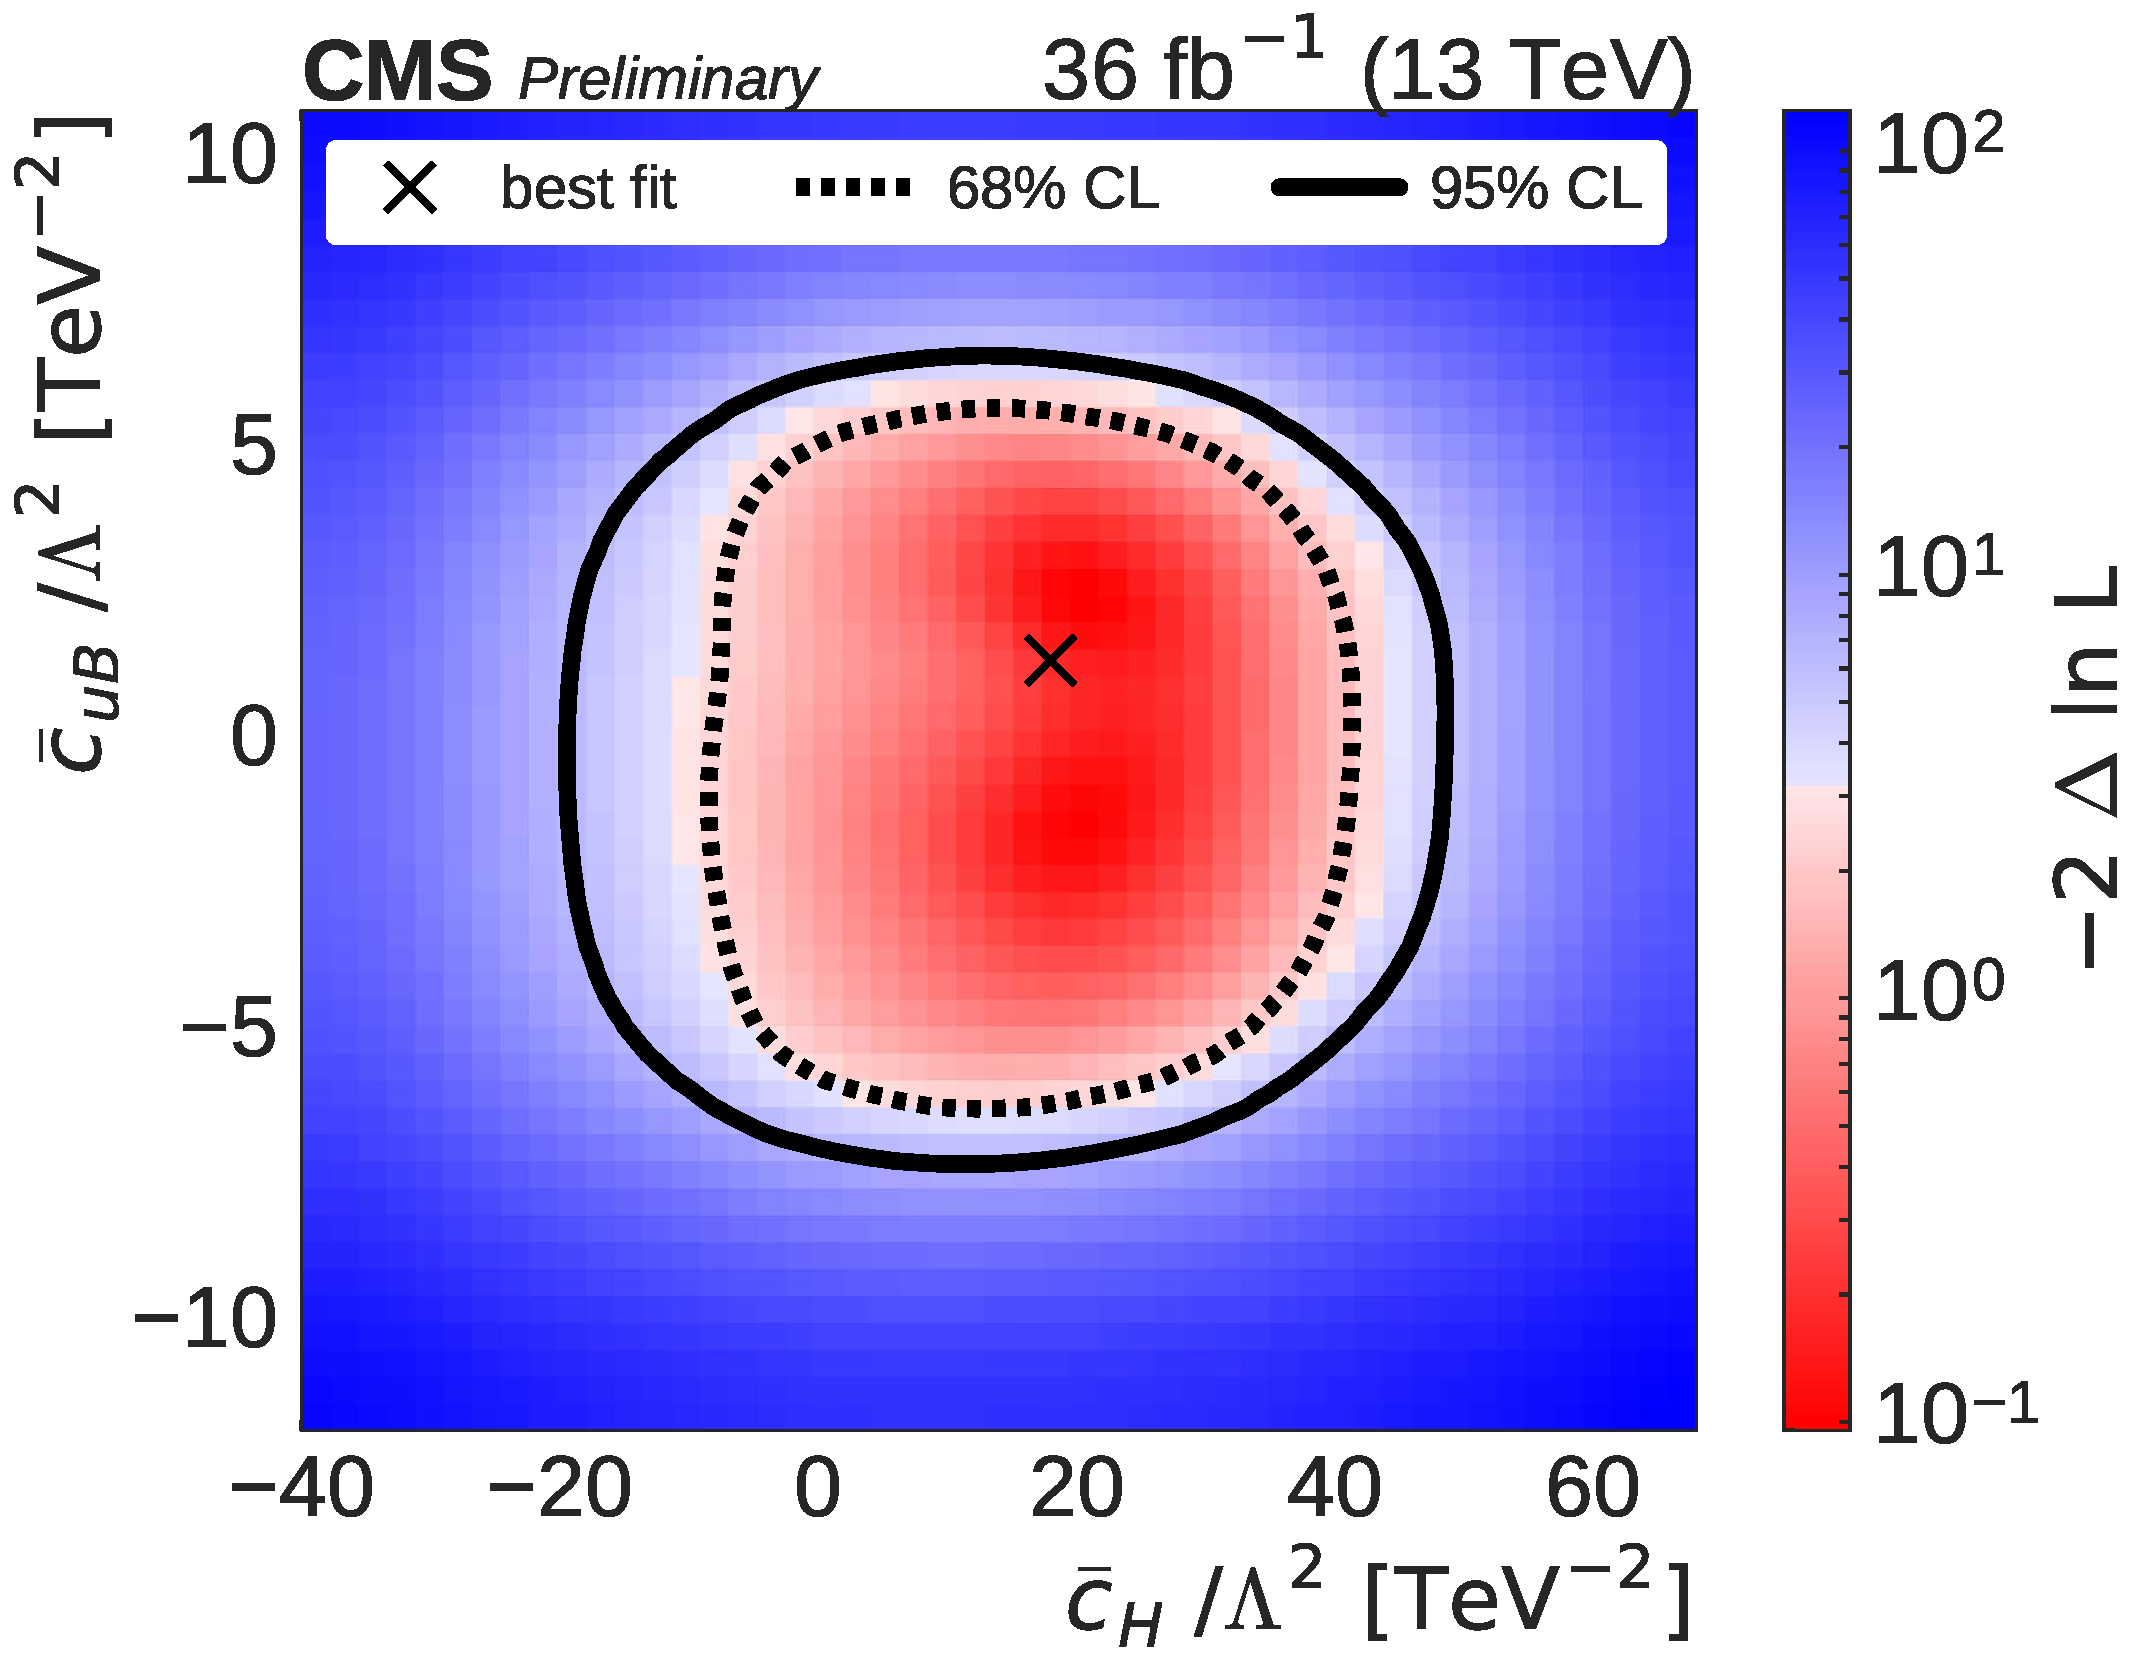
\includegraphics[width=0.6\linewidth]{figures/thirteen-TeV/nll/cH_cuB}
    \caption{}
  \end{subfigure}
  \vspace{-1cm}
  \setlength{\capwidth}{15cm}
  \caption[Signal scaling and profile likelihood scan in the \cH, \cuB plane]{Signal scaling shown
  in the \cH, \cuB plane with all other coefficients fixed to zero (a) or their best-fit values (b)
  for \ttZ (left), \ttH (center), and \ttW (right). The color represents the scaling ($\sigma_\text{NP
  + SM} / \sigma_\text{SM}$) due to NP effects. The star represents the SM point in which all $c_i=0$.
  The negative log likelihood is shown in (c). The best fit is represented by a cross. The
  \SI{68}{\percent} and \SI{95}{\percent} CL contours are shown with dashed and solid lines,
  respectively.}
\end{figure}

\begin{figure}
  \vspace{-1cm}
  \begin{subfigure}{\linewidth}
    \centering
    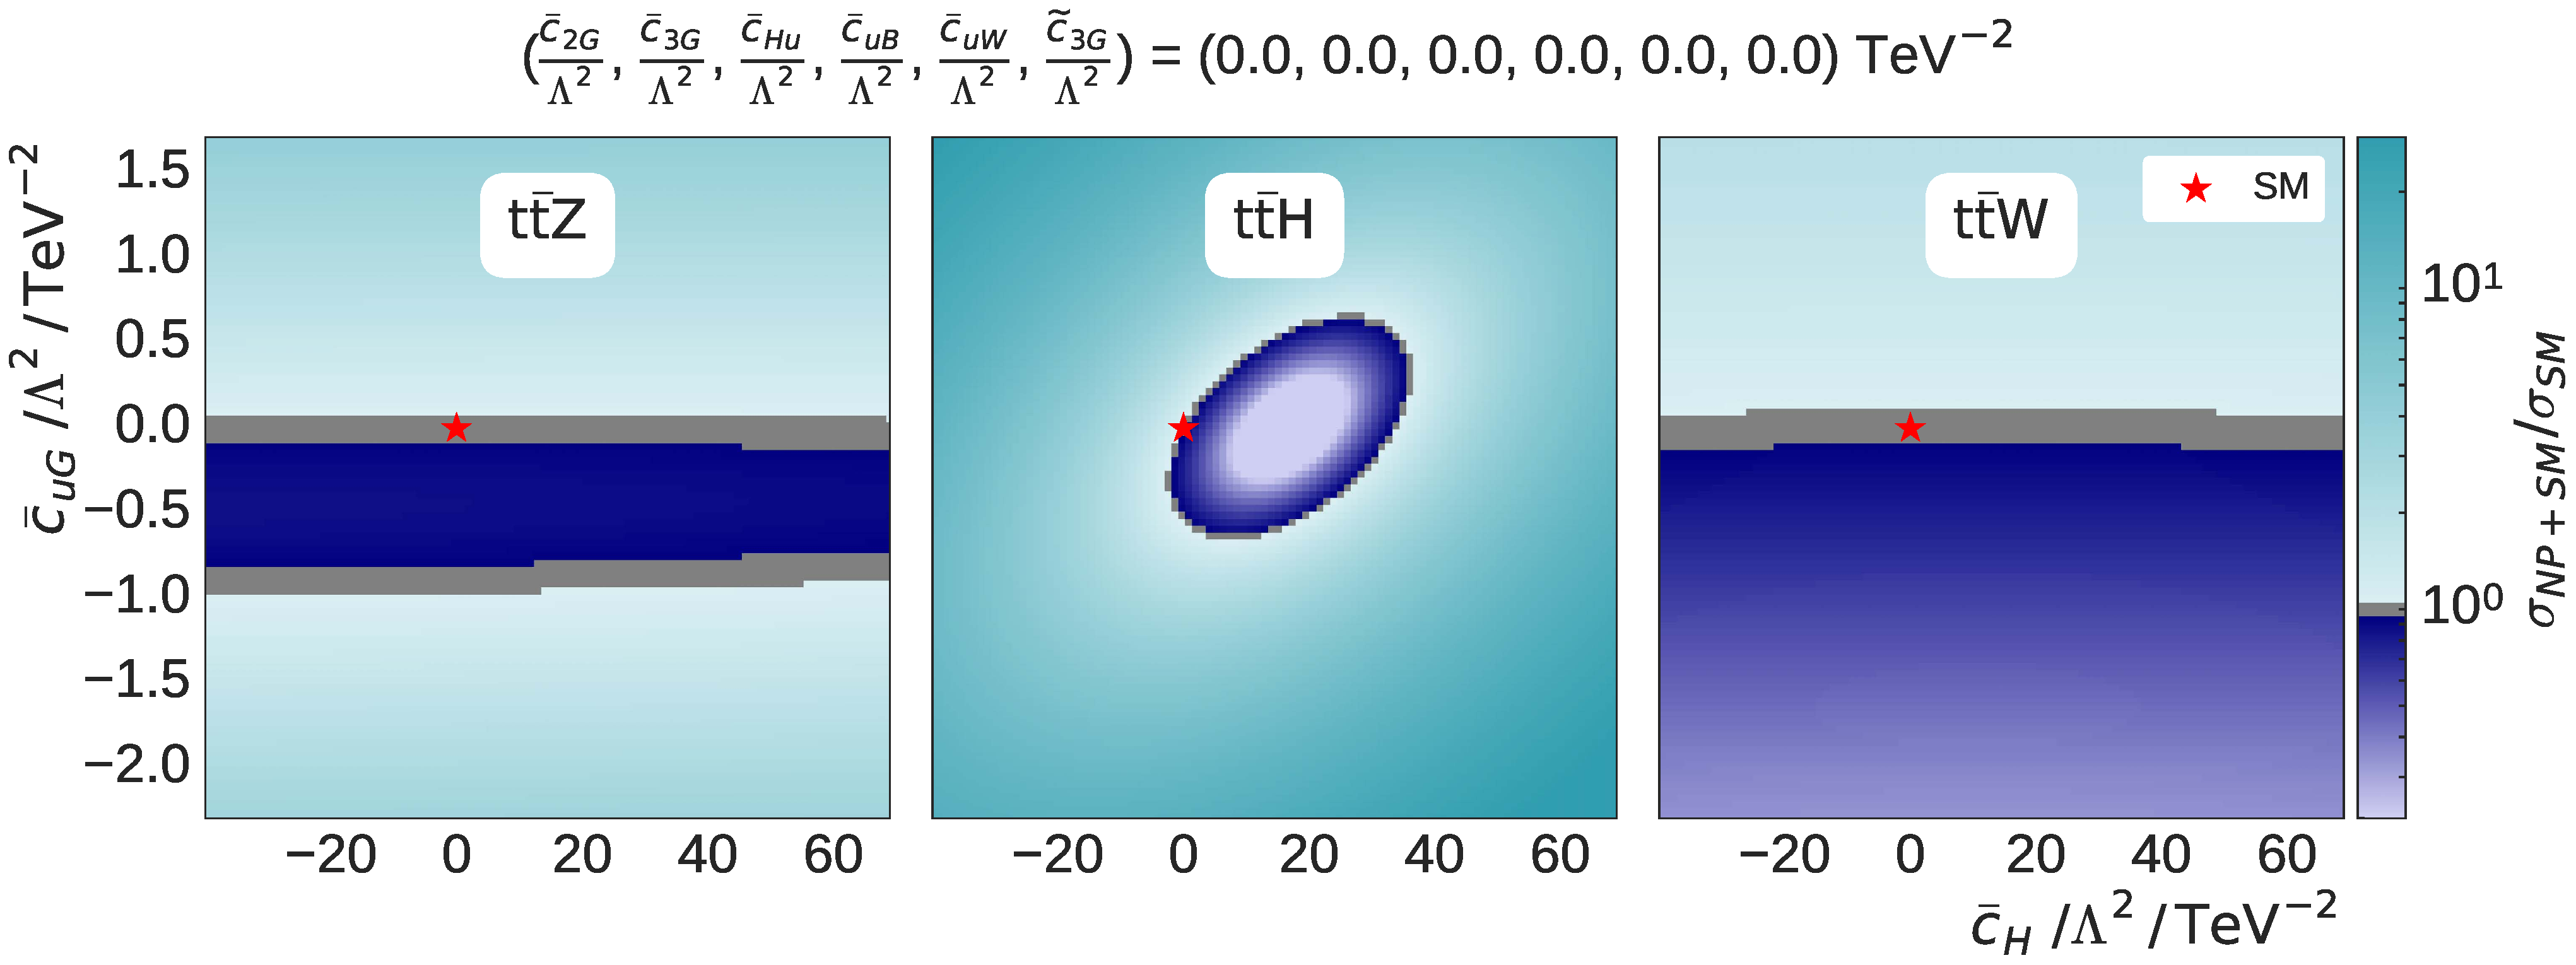
\includegraphics[width=\linewidth]{figures/thirteen-TeV/scaling-frozen/cH_cuG}
    \caption{}
  \end{subfigure}
  \begin{subfigure}{\linewidth}
    \centering
    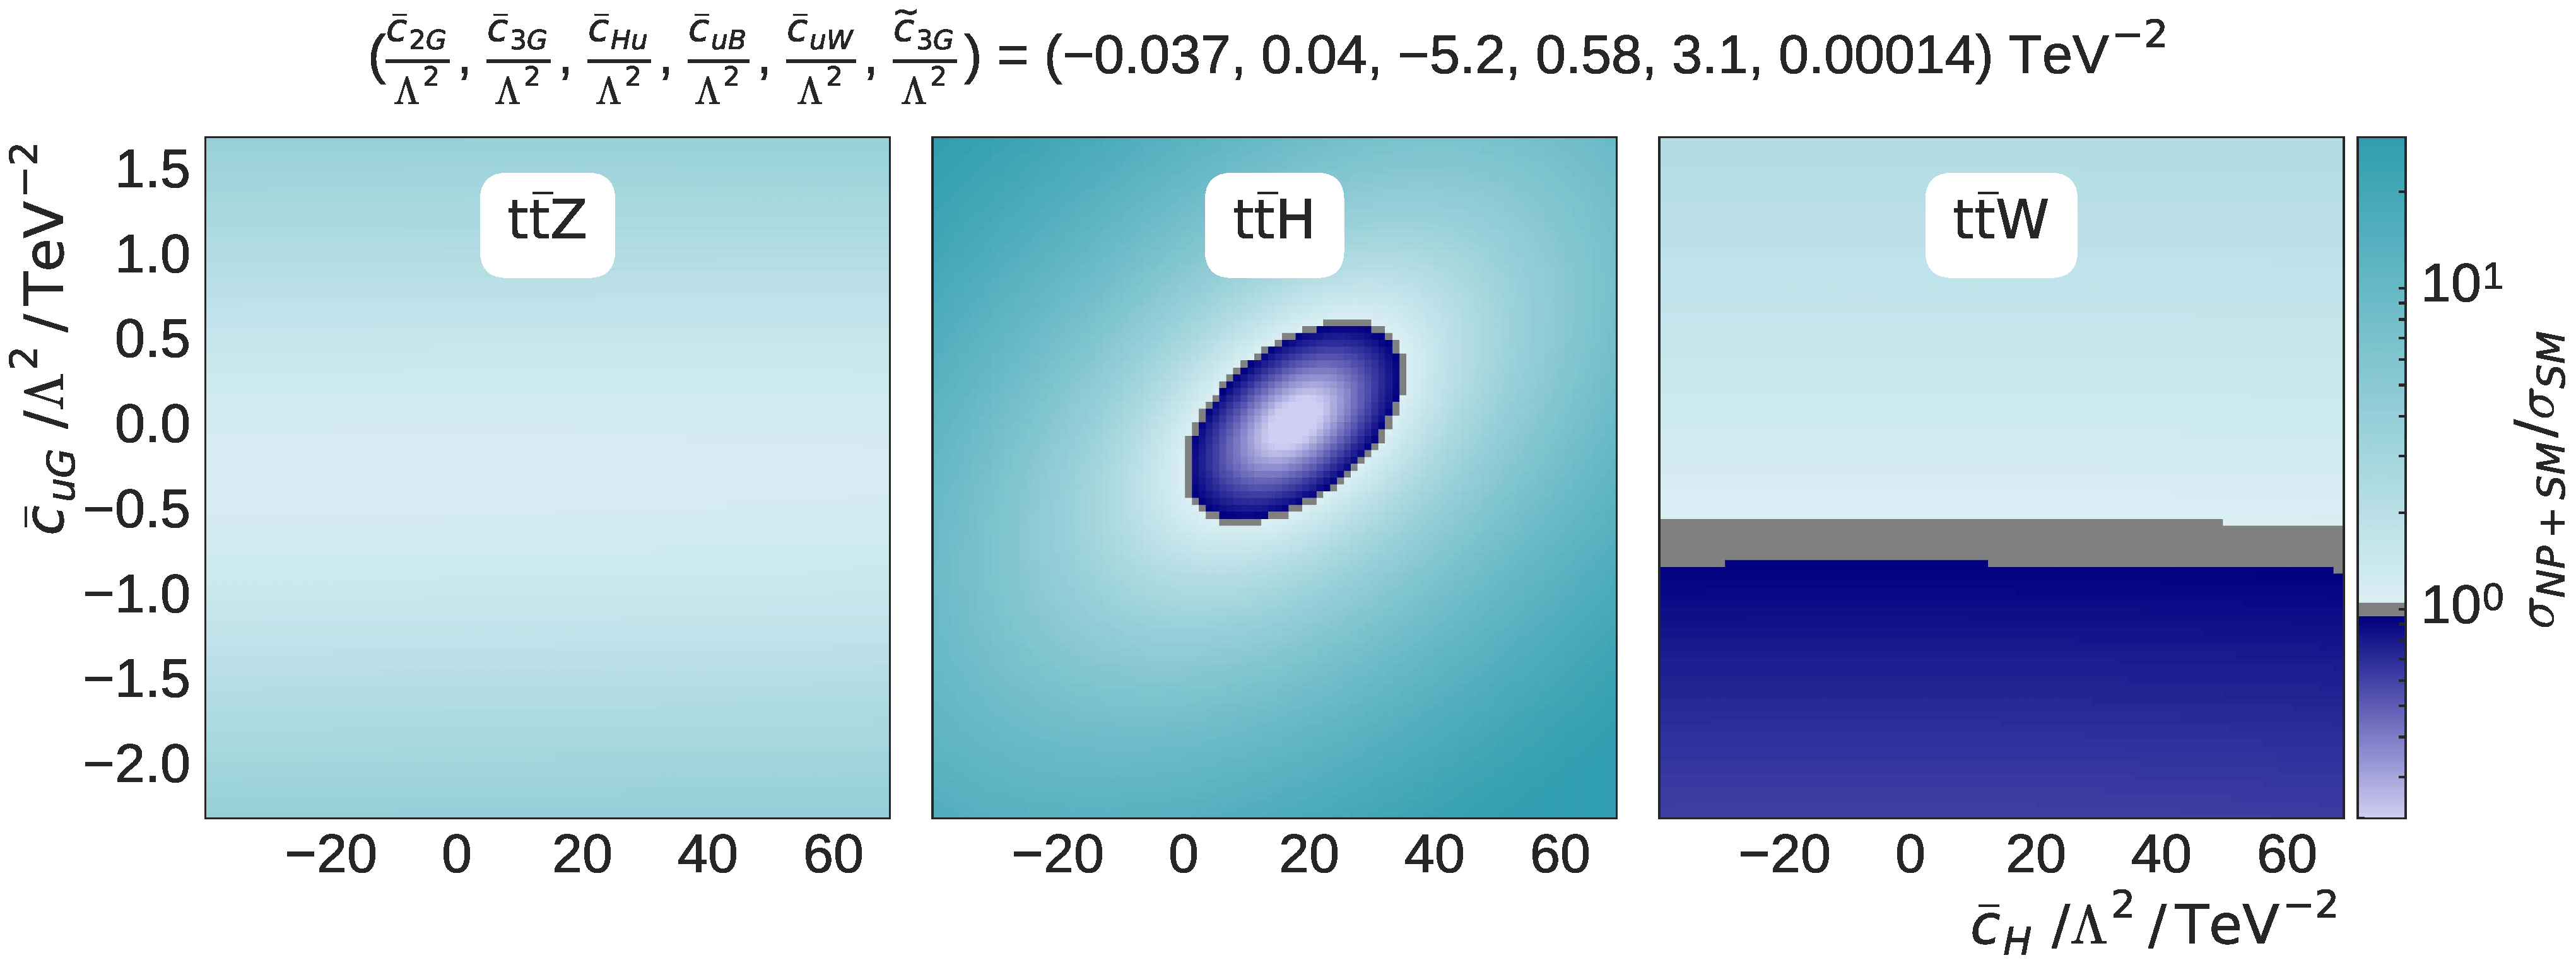
\includegraphics[width=\linewidth]{figures/thirteen-TeV/scaling/cH_cuG}
    \caption{}
  \end{subfigure}
  \begin{subfigure}{\linewidth}
    \centering
    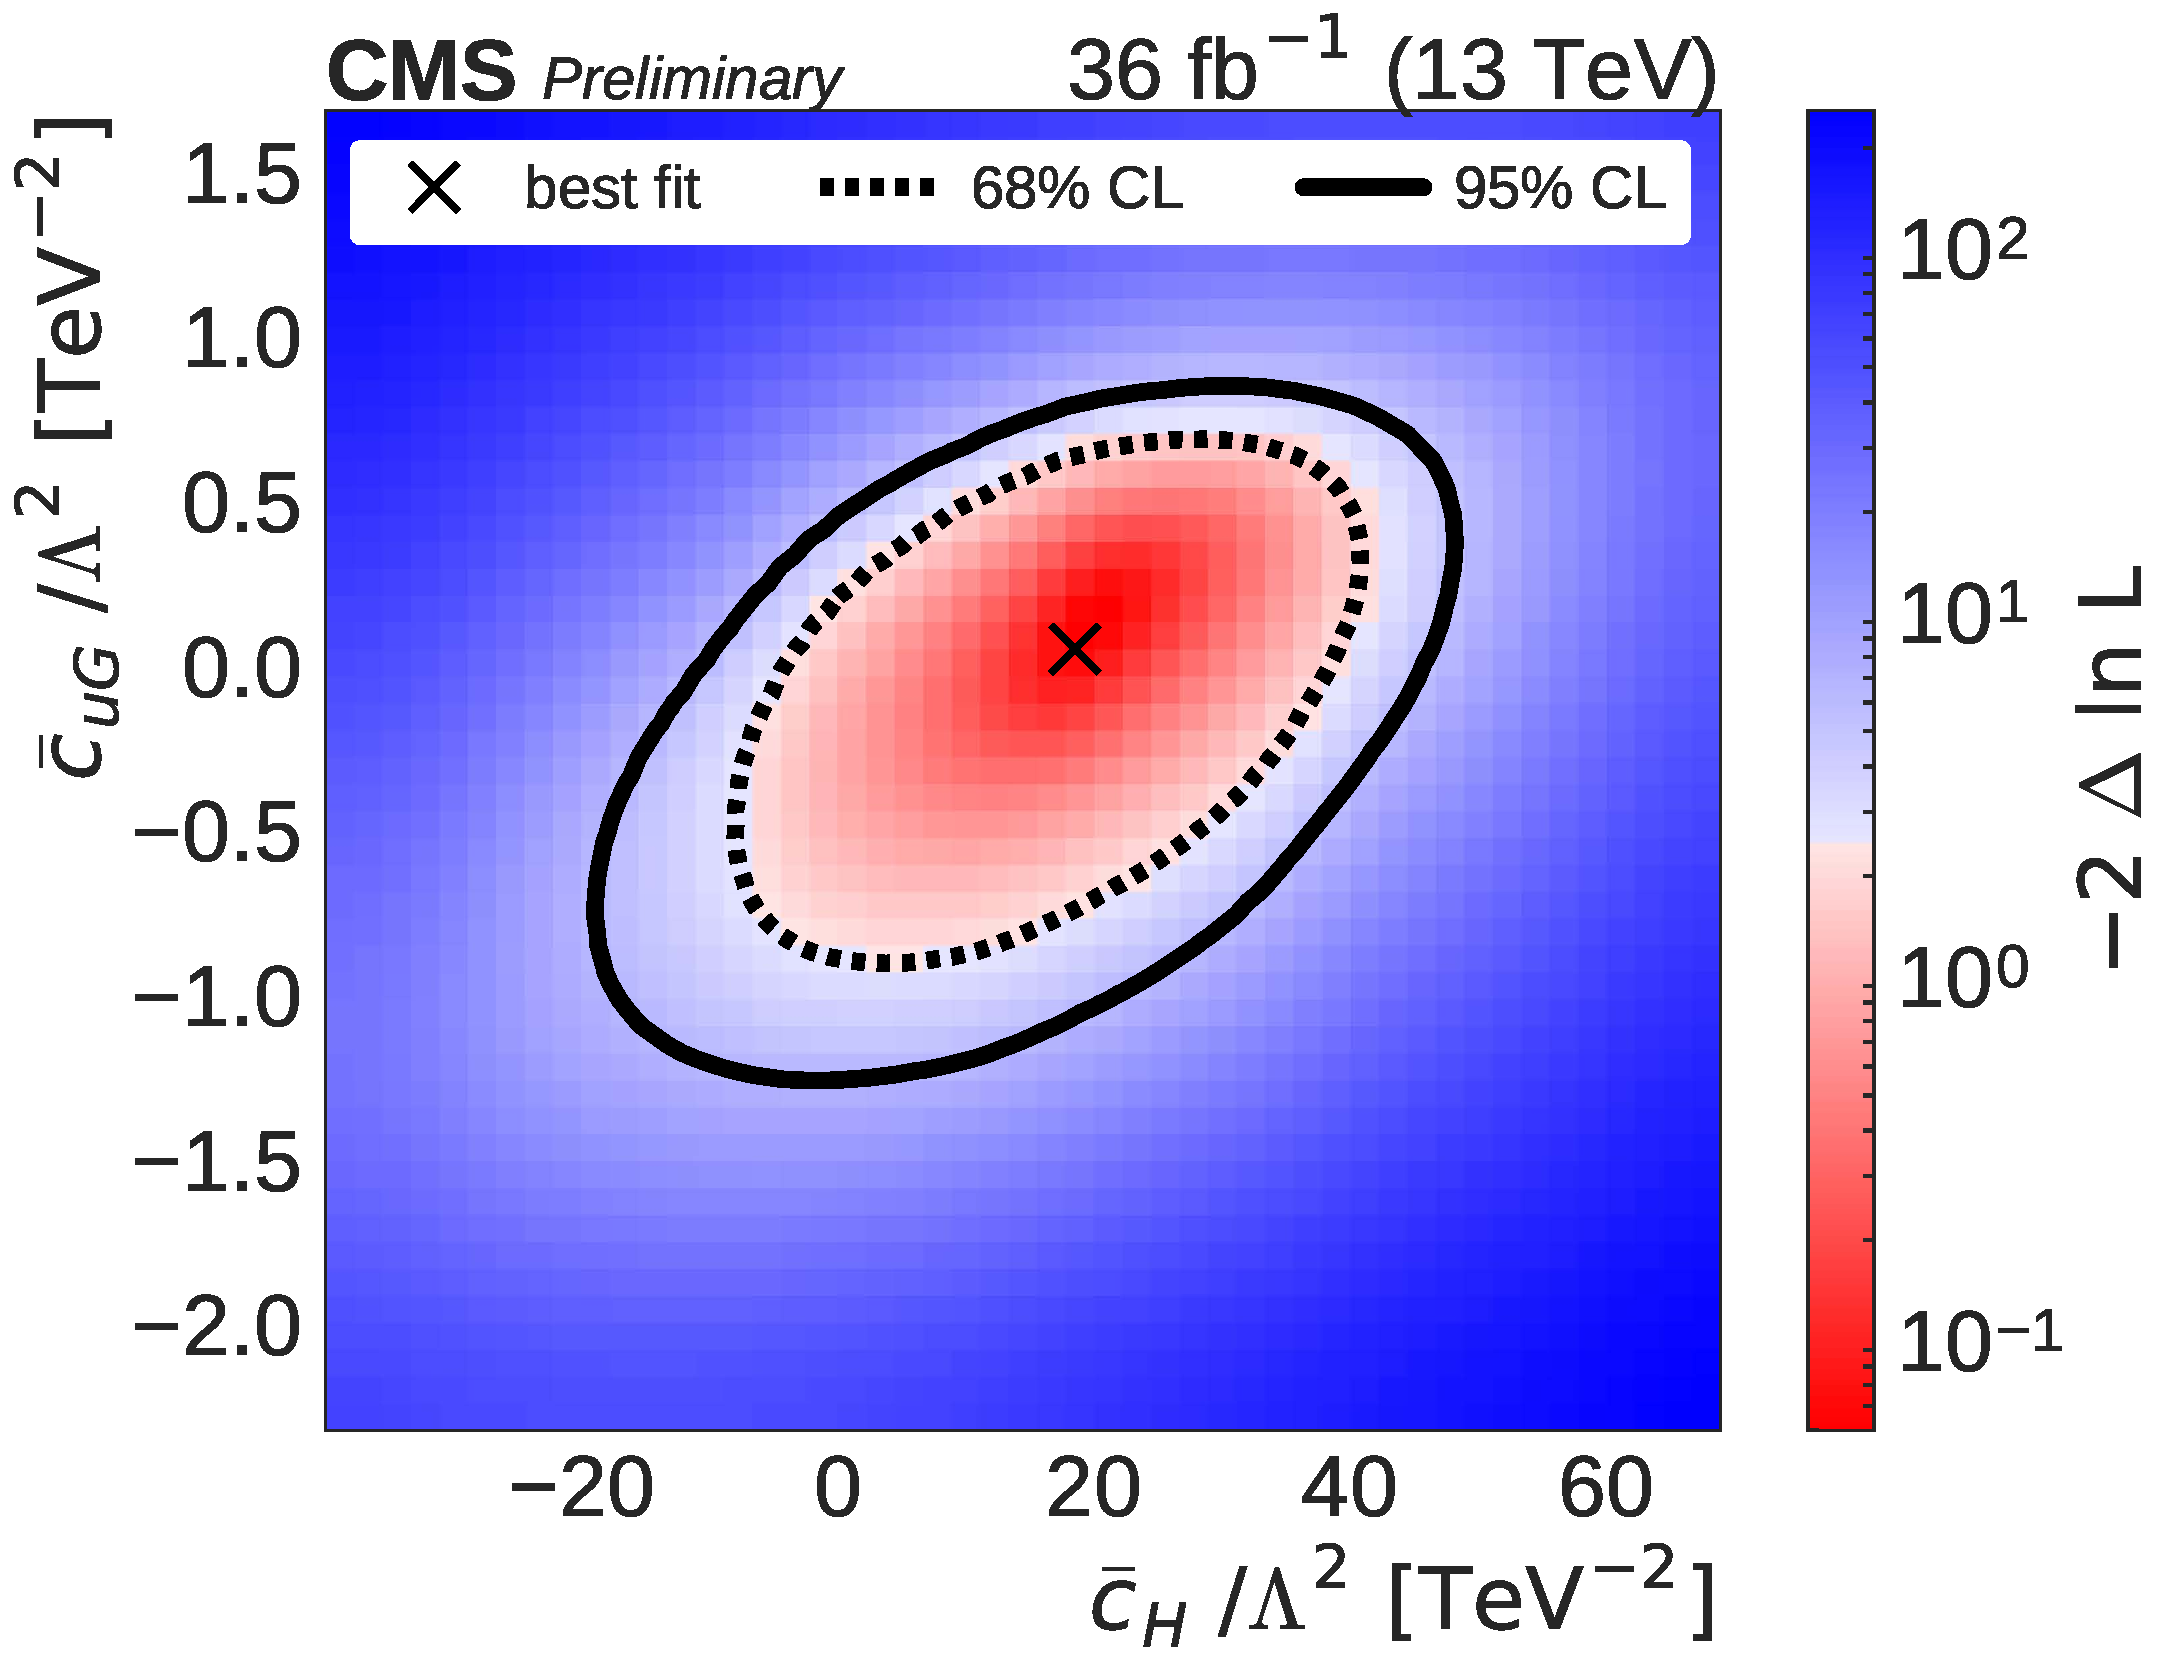
\includegraphics[width=0.6\linewidth]{figures/thirteen-TeV/nll/cH_cuG}
    \caption{}
  \end{subfigure}
  \vspace{-1cm}
  \setlength{\capwidth}{15cm}
  \caption[Signal scaling and profile likelihood scan in the \cH, \cuG plane]{Signal scaling shown
  in the \cH, \cuG plane with all other coefficients fixed to zero (a) or their best-fit values (b)
  for \ttZ (left), \ttH (center), and \ttW (right). The color represents the scaling ($\sigma_\text{NP
  + SM} / \sigma_\text{SM}$) due to NP effects. The star represents the SM point in which all $c_i=0$.
  The negative log likelihood is shown in (c). The best fit is represented by a cross. The
  \SI{68}{\percent} and \SI{95}{\percent} CL contours are shown with dashed and solid lines,
  respectively.}
\end{figure}

\begin{figure}
  \vspace{-1cm}
  \begin{subfigure}{\linewidth}
    \centering
    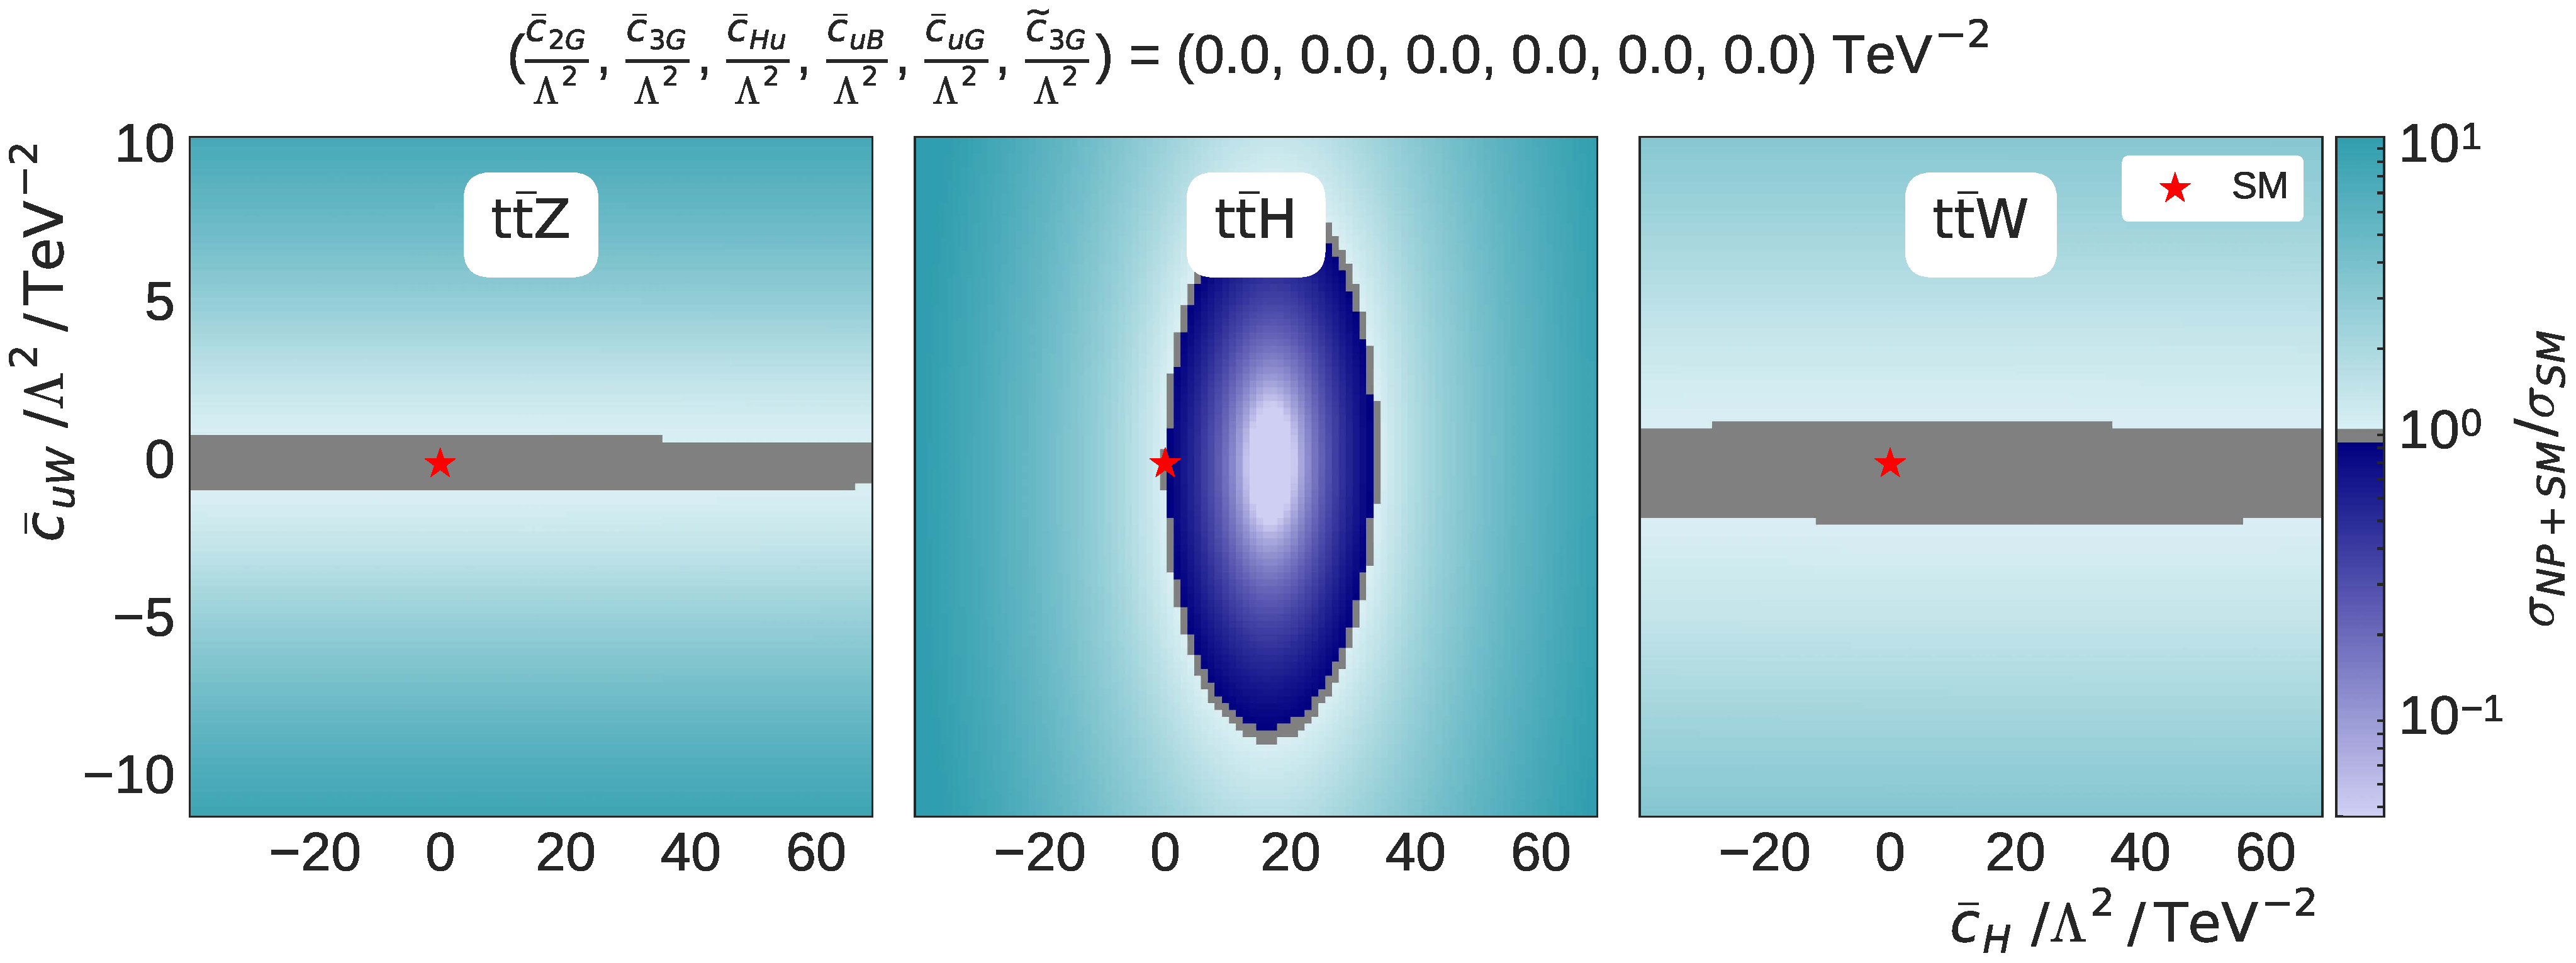
\includegraphics[width=\linewidth]{figures/thirteen-TeV/scaling-frozen/cH_cuW}
    \caption{}
  \end{subfigure}
  \begin{subfigure}{\linewidth}
    \centering
    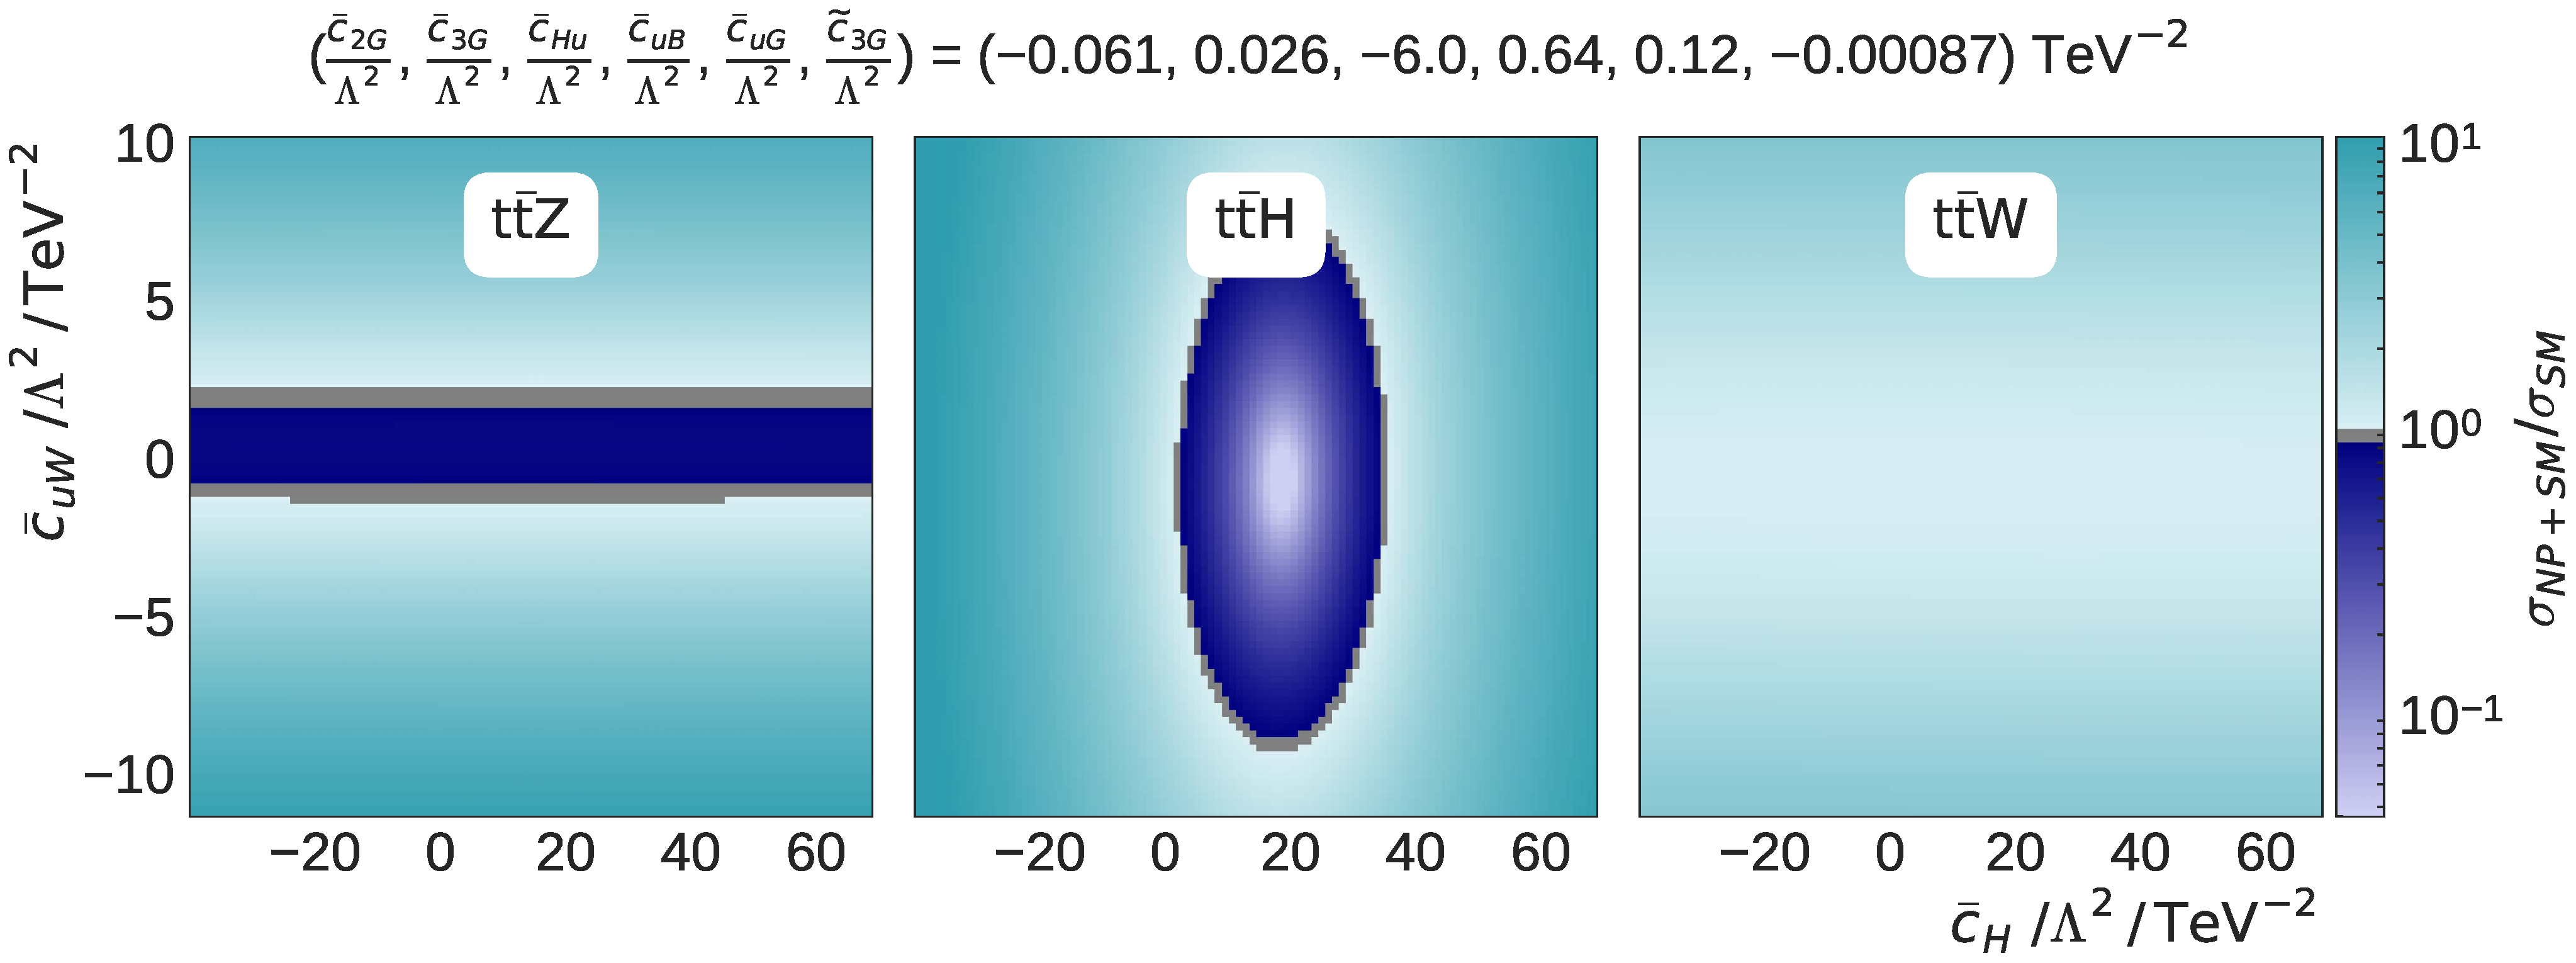
\includegraphics[width=\linewidth]{figures/thirteen-TeV/scaling/cH_cuW}
    \caption{}
  \end{subfigure}
  \begin{subfigure}{\linewidth}
    \centering
    \includegraphics[width=0.6\linewidth]{figures/thirteen-TeV/nll/cH_cuW}
    \caption{}
  \end{subfigure}
  \vspace{-1cm}
  \setlength{\capwidth}{15cm}
  \caption[Signal scaling and profile likelihood scan in the \cH, \cuW plane]{Signal scaling shown
  in the \cH, \cuW plane with all other coefficients fixed to zero (a) or their best-fit values (b)
  for \ttZ (left), \ttH (center), and \ttW (right). The color represents the scaling ($\sigma_\text{NP
  + SM} / \sigma_\text{SM}$) due to NP effects. The star represents the SM point in which all $c_i=0$.
  The negative log likelihood is shown in (c). The best fit is represented by a cross. The
  \SI{68}{\percent} and \SI{95}{\percent} CL contours are shown with dashed and solid lines,
  respectively.}
\end{figure}

\begin{figure}
  \vspace{-1cm}
  \begin{subfigure}{\linewidth}
    \centering
    \includegraphics[width=\linewidth]{figures/thirteen-TeV/scaling-frozen/cH_tc3G}
    \caption{}
  \end{subfigure}
  \begin{subfigure}{\linewidth}
    \centering
    \includegraphics[width=\linewidth]{figures/thirteen-TeV/scaling/cH_tc3G}
    \caption{}
  \end{subfigure}
  \begin{subfigure}{\linewidth}
    \centering
    \includegraphics[width=0.6\linewidth]{figures/thirteen-TeV/nll/cH_tc3G}
    \caption{}
  \end{subfigure}
  \vspace{-1cm}
  \setlength{\capwidth}{15cm}
  \caption[Signal scaling and profile likelihood scan in the \cH, \tcthreeG plane]{Signal scaling
  shown in the \cH, \tcthreeG plane with all other coefficients fixed to zero (a) or their best-fit
  values (b) for \ttZ (left), \ttH (center), and \ttW (right). The color represents the scaling
  ($\sigma_\text{NP + SM} / \sigma_\text{SM}$) due to NP effects. The star represents the SM point in
  which all $c_i=0$. The negative log likelihood is shown in (c). The best fit is represented by a
  cross. The \SI{68}{\percent} and \SI{95}{\percent} CL contours are shown with dashed and solid
  lines, respectively.}
\end{figure}

\begin{figure}
  \vspace{-1cm}
  \begin{subfigure}{\linewidth}
    \centering
    \includegraphics[width=\linewidth]{figures/thirteen-TeV/scaling-frozen/cuB_cuG}
    \caption{}
  \end{subfigure}
  \begin{subfigure}{\linewidth}
    \centering
    \includegraphics[width=\linewidth]{figures/thirteen-TeV/scaling/cuB_cuG}
    \caption{}
  \end{subfigure}
  \begin{subfigure}{\linewidth}
    \centering
    \includegraphics[width=0.6\linewidth]{figures/thirteen-TeV/nll/cuB_cuG}
    \caption{}
  \end{subfigure}
  \vspace{-1cm}
  \setlength{\capwidth}{15cm}
  \caption[Signal scaling and profile likelihood scan in the \cuB, \cuG plane]{Signal scaling shown
  in the \cuB, \cuG plane with all other coefficients fixed to zero (a) or their best-fit values (b)
  for \ttZ (left), \ttH (center), and \ttW (right). The color represents the scaling ($\sigma_\text{NP
  + SM} / \sigma_\text{SM}$) due to NP effects. The star represents the SM point in which all $c_i=0$.
  The negative log likelihood is shown in (c). The best fit is represented by a cross. The
  \SI{68}{\percent} and \SI{95}{\percent} CL contours are shown with dashed and solid lines,
  respectively.}
\end{figure}

\begin{figure}
  \vspace{-1cm}
  \begin{subfigure}{\linewidth}
    \centering
    \includegraphics[width=\linewidth]{figures/thirteen-TeV/scaling-frozen/cuB_cuW}
    \caption{}
  \end{subfigure}
  \begin{subfigure}{\linewidth}
    \centering
    \includegraphics[width=\linewidth]{figures/thirteen-TeV/scaling/cuB_cuW}
    \caption{}
  \end{subfigure}
  \begin{subfigure}{\linewidth}
    \centering
    \includegraphics[width=0.6\linewidth]{figures/thirteen-TeV/nll/cuB_cuW}
    \caption{}
  \end{subfigure}
  \vspace{-1cm}
  \setlength{\capwidth}{15cm}
  \caption[Signal scaling and profile likelihood scan in the \cuB, \cuW plane]{Signal scaling shown
  in the \cuB, \cuW plane with all other coefficients fixed to zero (a) or their best-fit values (b)
  for \ttZ (left), \ttH (center), and \ttW (right). The color represents the scaling ($\sigma_\text{NP
  + SM} / \sigma_\text{SM}$) due to NP effects. The star represents the SM point in which all $c_i=0$.
  The negative log likelihood is shown in (c). The best fit is represented by a cross. The
  \SI{68}{\percent} and \SI{95}{\percent} CL contours are shown with dashed and solid lines,
  respectively.}
\end{figure}

\begin{figure}
  \vspace{-1cm}
  \begin{subfigure}{\linewidth}
    \centering
    \includegraphics[width=\linewidth]{figures/thirteen-TeV/scaling-frozen/cuB_tc3G}
    \caption{}
  \end{subfigure}
  \begin{subfigure}{\linewidth}
    \centering
    \includegraphics[width=\linewidth]{figures/thirteen-TeV/scaling/cuB_tc3G}
    \caption{}
  \end{subfigure}
  \begin{subfigure}{\linewidth}
    \centering
    \includegraphics[width=0.6\linewidth]{figures/thirteen-TeV/nll/cuB_tc3G}
    \caption{}
  \end{subfigure}
  \vspace{-1cm}
  \setlength{\capwidth}{15cm}
  \caption[Signal scaling and profile likelihood scan in the \cuB, \tcthreeG plane]{Signal scaling
  shown in the \cuB, \tcthreeG plane with all other coefficients fixed to zero (a) or their best-fit
  values (b) for \ttZ (left), \ttH (center), and \ttW (right). The color represents the scaling
  ($\sigma_\text{NP + SM} / \sigma_\text{SM}$) due to NP effects. The star represents the SM point in
  which all $c_i=0$. The negative log likelihood is shown in (c). The best fit is represented by a
  cross. The \SI{68}{\percent} and \SI{95}{\percent} CL contours are shown with dashed and solid
  lines, respectively.}
\end{figure}

\begin{figure}
  \vspace{-1cm}
  \begin{subfigure}{\linewidth}
    \centering
    \includegraphics[width=\linewidth]{figures/thirteen-TeV/scaling-frozen/cuG_cuW}
    \caption{}
  \end{subfigure}
  \begin{subfigure}{\linewidth}
    \centering
    \includegraphics[width=\linewidth]{figures/thirteen-TeV/scaling/cuG_cuW}
    \caption{}
  \end{subfigure}
  \begin{subfigure}{\linewidth}
    \centering
    \includegraphics[width=0.6\linewidth]{figures/thirteen-TeV/nll/cuG_cuW}
    \caption{}
  \end{subfigure}
  \vspace{-1cm}
  \setlength{\capwidth}{15cm}
  \caption[Signal scaling and profile likelihood scan in the \cuG, \cuW plane]{Signal scaling shown
  in the \cuG, \cuW plane with all other coefficients fixed to zero (a) or their best-fit values (b)
  for \ttZ (left), \ttH (center), and \ttW (right). The color represents the scaling ($\sigma_\text{NP
  + SM} / \sigma_\text{SM}$) due to NP effects. The star represents the SM point in which all $c_i=0$.
  The negative log likelihood is shown in (c). The best fit is represented by a cross. The
  \SI{68}{\percent} and \SI{95}{\percent} CL contours are shown with dashed and solid lines,
  respectively.}
\end{figure}

\begin{figure}
  \vspace{-1cm}
  \begin{subfigure}{\linewidth}
    \centering
    \includegraphics[width=\linewidth]{figures/thirteen-TeV/scaling-frozen/cuG_tc3G}
    \caption{}
  \end{subfigure}
  \begin{subfigure}{\linewidth}
    \centering
    \includegraphics[width=\linewidth]{figures/thirteen-TeV/scaling/cuG_tc3G}
    \caption{}
  \end{subfigure}
  \begin{subfigure}{\linewidth}
    \centering
    \includegraphics[width=0.6\linewidth]{figures/thirteen-TeV/nll/cuG_tc3G}
    \caption{}
  \end{subfigure}
  \vspace{-1cm}
  \setlength{\capwidth}{15cm}
  \caption[Signal scaling and profile likelihood scan in the \cuG, \tcthreeG plane]{Signal scaling
  shown in the \cuG, \tcthreeG plane with all other coefficients fixed to zero (a) or their best-fit
  values (b) for \ttZ (left), \ttH (center), and \ttW (right). The color represents the scaling
  ($\sigma_\text{NP + SM} / \sigma_\text{SM}$) due to NP effects. The star represents the SM point in
  which all $c_i=0$. The negative log likelihood is shown in (c). The best fit is represented by a
  cross. The \SI{68}{\percent} and \SI{95}{\percent} CL contours are shown with dashed and solid
  lines, respectively.}
\end{figure}

\begin{figure}
  \vspace{-1cm}
  \begin{subfigure}{\linewidth}
    \centering
    \includegraphics[width=\linewidth]{figures/thirteen-TeV/scaling-frozen/cuW_tc3G}
    \caption{}
  \end{subfigure}
  \begin{subfigure}{\linewidth}
    \centering
    \includegraphics[width=\linewidth]{figures/thirteen-TeV/scaling/cuW_tc3G}
    \caption{}
  \end{subfigure}
  \begin{subfigure}{\linewidth}
    \centering
    \includegraphics[width=0.6\linewidth]{figures/thirteen-TeV/nll/cuW_tc3G}
    \caption{}
  \end{subfigure}
  \vspace{-1cm}
  \setlength{\capwidth}{15cm}
  \caption[Signal scaling and profile likelihood scan in the \cuW, \tcthreeG plane]{Signal scaling
  shown in the \cuW, \tcthreeG plane with all other coefficients fixed to zero (a) or their best-fit
  values (b) for \ttZ (left), \ttH (center), and \ttW (right). The color represents the scaling
  ($\sigma_\text{NP + SM} / \sigma_\text{SM}$) due to NP effects. The star represents the SM point in
  which all $c_i=0$. The negative log likelihood is shown in (c). The best fit is represented by a
  cross. The \SI{68}{\percent} and \SI{95}{\percent} CL contours are shown with dashed and solid
  lines, respectively.}
\end{figure}
